\documentclass[twoside]{book}

% Packages required by doxygen
\usepackage{fixltx2e}
\usepackage{calc}
\usepackage{doxygen}
\usepackage[export]{adjustbox} % also loads graphicx
\usepackage{graphicx}
\usepackage[utf8]{inputenc}
\usepackage{makeidx}
\usepackage{multicol}
\usepackage{multirow}
\PassOptionsToPackage{warn}{textcomp}
\usepackage{textcomp}
\usepackage[nointegrals]{wasysym}
\usepackage[table]{xcolor}

% Font selection
\usepackage[T1]{fontenc}
\usepackage[scaled=.90]{helvet}
\usepackage{courier}
\usepackage{amssymb}
\usepackage{sectsty}
\renewcommand{\familydefault}{\sfdefault}
\allsectionsfont{%
  \fontseries{bc}\selectfont%
  \color{darkgray}%
}
\renewcommand{\DoxyLabelFont}{%
  \fontseries{bc}\selectfont%
  \color{darkgray}%
}
\newcommand{\+}{\discretionary{\mbox{\scriptsize$\hookleftarrow$}}{}{}}

% Page & text layout
\usepackage{geometry}
\geometry{%
  a4paper,%
  top=2.5cm,%
  bottom=2.5cm,%
  left=2.5cm,%
  right=2.5cm%
}
\tolerance=750
\hfuzz=15pt
\hbadness=750
\setlength{\emergencystretch}{15pt}
\setlength{\parindent}{0cm}
\setlength{\parskip}{3ex plus 2ex minus 2ex}
\makeatletter
\renewcommand{\paragraph}{%
  \@startsection{paragraph}{4}{0ex}{-1.0ex}{1.0ex}{%
    \normalfont\normalsize\bfseries\SS@parafont%
  }%
}
\renewcommand{\subparagraph}{%
  \@startsection{subparagraph}{5}{0ex}{-1.0ex}{1.0ex}{%
    \normalfont\normalsize\bfseries\SS@subparafont%
  }%
}
\makeatother

% Headers & footers
\usepackage{fancyhdr}
\pagestyle{fancyplain}
\fancyhead[LE]{\fancyplain{}{\bfseries\thepage}}
\fancyhead[CE]{\fancyplain{}{}}
\fancyhead[RE]{\fancyplain{}{\bfseries\leftmark}}
\fancyhead[LO]{\fancyplain{}{\bfseries\rightmark}}
\fancyhead[CO]{\fancyplain{}{}}
\fancyhead[RO]{\fancyplain{}{\bfseries\thepage}}
\fancyfoot[LE]{\fancyplain{}{}}
\fancyfoot[CE]{\fancyplain{}{}}
\fancyfoot[RE]{\fancyplain{}{\bfseries\scriptsize Generated by Doxygen }}
\fancyfoot[LO]{\fancyplain{}{\bfseries\scriptsize Generated by Doxygen }}
\fancyfoot[CO]{\fancyplain{}{}}
\fancyfoot[RO]{\fancyplain{}{}}
\renewcommand{\footrulewidth}{0.4pt}
\renewcommand{\chaptermark}[1]{%
  \markboth{#1}{}%
}
\renewcommand{\sectionmark}[1]{%
  \markright{\thesection\ #1}%
}

% Indices & bibliography
\usepackage{natbib}
\usepackage[titles]{tocloft}
\setcounter{tocdepth}{3}
\setcounter{secnumdepth}{5}
\makeindex

% Hyperlinks (required, but should be loaded last)
\usepackage{ifpdf}
\ifpdf
  \usepackage[pdftex,pagebackref=true]{hyperref}
\else
  \usepackage[ps2pdf,pagebackref=true]{hyperref}
\fi
\hypersetup{%
  colorlinks=true,%
  linkcolor=blue,%
  citecolor=blue,%
  unicode%
}

% Custom commands
\newcommand{\clearemptydoublepage}{%
  \newpage{\pagestyle{empty}\cleardoublepage}%
}

\usepackage{caption}
\captionsetup{labelsep=space,justification=centering,font={bf},singlelinecheck=off,skip=4pt,position=top}

%===== C O N T E N T S =====

\begin{document}

% Titlepage & ToC
\hypersetup{pageanchor=false,
             bookmarksnumbered=true,
             pdfencoding=unicode
            }
\pagenumbering{roman}
\begin{titlepage}
\vspace*{7cm}
\begin{center}%
{\Large framework\+\_\+\+Jin-\/new\+\_\+server }\\
\vspace*{1cm}
{\large Generated by Doxygen 1.8.11}\\
\end{center}
\end{titlepage}
\clearemptydoublepage
\tableofcontents
\clearemptydoublepage
\pagenumbering{arabic}
\hypersetup{pageanchor=true}

%--- Begin generated contents ---
\chapter{Documentation for the whole program}
\label{index}\hypertarget{index}{}\subsection*{How to use}

Open the Sever(first)\+: \begin{DoxyVerb}open the agentSim(home/CLionProject/framework_jin)
\end{DoxyVerb}


Virtual Car(home/mkz-\/mpc-\/control/output.\+txt) (optional)\+: \begin{DoxyVerb}Each row: current car number & first car id & first car x & first car y & first car angle & first car vx first car vy & first car angular v & second ….
0.1 s update one row.
If fisrt three col is 0 (x,y,angle) —> car disappear.

To add the virtual car, click "Startvc" at the manager website.
To start it, click "Start" at the manager website.(If you have started it once, you don't need to do this again.)
\end{DoxyVerb}


Human Car(optional)\+: \begin{DoxyVerb}(1) Initial steel, brake, accelerator : Desktop: FFB_Cs ——> initDevice ——> start
(2) Send car info(steel, brake, accelerator) to server: Desktop/Fan/MscArch/UDP_project/UDP_proecjt.sln ——> run
(3) Rendering(渲染): D:/sim/11.13/Rending(network)/launch.ps1
(4) Chose the agenttype as FourWheelCar and type in the initial states, click "add" at the manager website.
(5) To start it, click "Start" at the manager website.(If you have started it once, you don't need to do this again.)

How to create a new map (rendering) : D:/sim/11.13/12.13/MyProejct/MyProject.uproject
    Change IP address: open .sln (need to rebuild solution and new to create a new rendering)
    Unreal4 (how to create road in unreal4 )
    after modify, create a new rendering: File -> Package Project -> windows -> 64bit ———> create a new folder called windowNoEditor
    Copy all file under windowNoEditor to D:/sim/11.13/Rendering(network)/ front, left, right (replace)
    How to connect with server: MyProject.sln/ Game
\end{DoxyVerb}


Real Car(optional)\+: \begin{DoxyVerb}(1) Collect data from real car: home/mkz-mpc-control ——> open power shell ——> source devel/setup.sh ———> rosrun collect collect_node (For real car)  and then use manager addRealCar
(2) Chose the agenttype as RealCar and type in the initial states, click "add" at the manager website.
(3) To start it, click "Start" at the manager website.(If you have started it once, you don't need to do this again.)
\end{DoxyVerb}


\subsection*{How the Main thread Work}

When you run the server, it will creat a thread pool include 10 threads for simulator to calculate agents. The thread pool will open one extra thread to manage these 10 threads automatically.

Then, it will creat a simulator and a server. The simulator and the server will share their Simulator\+State, Agent\+Dictionary and human\+Inputs, so that the manager can manage the simulator. And, other session can get what they need. The server will sign three kinds of services for for input, manager and rendering and open 5 threads to waiting for the command.

At last, it will invoke simulator\+::run which is a endless loop to update the simulator.

\subsection*{Documents}

If you change some documents and want to regenerate the document. Remember to change the address in the Doxyfile. 
\chapter{Documentation for custom class derived from `\+Controller`}
\label{md_README-controller}
\hypertarget{md_README-controller}{}
\subsection*{Header files}

Please include {\ttfamily Controller/\+Controller.\+hpp} before you derive your custome class from {\ttfamily \hyperlink{classController}{Controller}}. 
\begin{DoxyCode}
1 \{C++\}
2 #include "Controller/Controller.hpp"
3 class MyController : public Controller \{
4     // definition body ...
5 \}
\end{DoxyCode}


\subsection*{Construction}

You are supposed to specify the dimension of {\ttfamily state} vector and {\ttfamily input} vector in the argument list of the construction of the base class {\ttfamily \hyperlink{classPlanner}{Planner}}. For example, if we want to derive a {\ttfamily \hyperlink{classHumanCarPlanner}{Human\+Car\+Planner}} class, we should write the construction as follows\+: 
\begin{DoxyCode}
1 \{C++\}
2 MyController::MyController(/* your argument list here */) : Planner(d, 3) \{
3     // construction body ...
4 \}
\end{DoxyCode}
 since we have an intermediate vector of dimension 3 (gas pedal, brake pedal, steering wheel angle), and an input vector of dimension d (the {\ttfamily input} vector is the output of Zeji\textquotesingle{}s planner).

\subsection*{Overriding the virtual method}

All the interface of a {\ttfamily \hyperlink{classController}{Controller}} lies in the virtual method {\ttfamily update}. The signature of this function is\+: 
\begin{DoxyCode}
1 \{C++\}
2 typedef std::vector<double> Vector;
3 Vector HumanCarController::update(Vector input);
\end{DoxyCode}


It takes {\ttfamily input} vector, which is the output of Zeji\textquotesingle{}s planner. The return vector should be the intermediate vector, which is gas pedal, brake pedal, and steering angle.

For each agent, there is a {\ttfamily get\+State()} method, which gives the state vector of this agent. For a car, this state vector has 6 dimensions\+: location x, location y, yaw angle, speed x, speed y, angular velocity of yaw. You can use {\ttfamily agents} to get information of the environment.

\subsection*{Exception handling}

If the dimensions of the vectors do not match, an {\ttfamily std\+::runtime\+\_\+error} will be thrown. For example, if we give a 5-\/dimension vector {\ttfamily state} to our {\ttfamily \hyperlink{classHumanCarPlanner}{Human\+Car\+Planner}}, which expects a 6-\/dimension state vector\+: 
\begin{DoxyCode}
1 \{C++\}
2 try \{
3     Vector currentState = Vector \{0, 0, 0, 1, 2\}; // 5-dimension state vector
4     Vector input = MyPlanner.update(currentState, humanInput, agents); // HumanCar expects 6-dimension
       state vector
5     MyController.update(input);
6 \}
7 catch (std::runtime\_error e) \{
8     std::cout << e.what() << std::endl;
9 \}
\end{DoxyCode}
 
\chapter{Documentation for custom class derived from `\+Planner`}
\label{md_README-planner}
\hypertarget{md_README-planner}{}
\subsection*{Header files}

Please include {\ttfamily \hyperlink{Planner_8hpp}{Planners/\+Planner.\+hpp}} before you derive your custome class from {\ttfamily \hyperlink{classPlanner}{Planner}}. 
\begin{DoxyCode}
1 \{C++\}
2 #include "Planners/Planner.hpp"
3 class MyPlanner : public Planner \{
4     // definition body ...
5 \}
\end{DoxyCode}


\subsection*{Construction}

You are supposed to specify the dimension of {\ttfamily state} vector and {\ttfamily input} vector in the argument list of the construction of the base class {\ttfamily \hyperlink{classPlanner}{Planner}}. For example, if we want to derive a {\ttfamily My\+Planner} class, we should write the construction as follows\+: 
\begin{DoxyCode}
1 \{C++\}
2 MyPlanner::MyPlanner(/* your argument list here */) : Planner(6, d) \{
3     // construction body ...
4 \}
\end{DoxyCode}
 since a {\ttfamily \hyperlink{classHumanCar}{Human\+Car}} has a state vector of dimension 6 (location X, location Y, yaw angle, speed X, speed Y, angular speed of yaw), and an input vector of dimension d (the {\ttfamily input} vector is the output of Zeji\textquotesingle{}s planner).

\subsection*{Overriding the virtual method}

All the interface of a {\ttfamily \hyperlink{classPlanner}{Planner}} lies in the virtual method {\ttfamily update}. The signature of this function is\+: 
\begin{DoxyCode}
1 \{C++\}
2 typedef std::vector<double> Vector;
3 Vector Planner::update(Vector currentState, const Vector &humanInput, std::vector<Agent*> agents);
\end{DoxyCode}


It takes input of the current state of the agent, the human input (if your planner needs it), and information of other agents. It will have the fourth argument {\ttfamily Environment} in future versions, but right now we do not have this parameter.

It outputs the input vector, which the simulator will pass to the agent controller and use it to update the agent state for the next iteration.

For example, for the \hyperlink{classHumanCar}{Human\+Car}, we should write our overridden implementation as\+: 
\begin{DoxyCode}
1 \{C++\}
2 Vector HumanCarPlanner::update(Vector currentState, const Vector &humanInput, std::vector<Agent*> agents) \{
3     return Vector(humanInput); // directly use the human input for the planner output
4 \}
\end{DoxyCode}


\subsection*{If you need information of other agents...}

For each agent, there is a {\ttfamily get\+State()} method, which gives the state vector of this agent. For a car, this state vector has 6 dimensions\+: location x, location y, yaw angle, speed x, speed y, angular velocity of yaw. You can use the vector {\ttfamily agents} to get information of the environment.

\subsection*{Exception handling}

If the dimensions of the vectors do not match, an {\ttfamily std\+::runtime\+\_\+error} will be thrown. For example, if we give a 5-\/dimension vector {\ttfamily state} to our {\ttfamily \hyperlink{classHumanCarPlanner}{Human\+Car\+Planner}}, which expects a 6-\/dimension state vector\+: 
\begin{DoxyCode}
1 \{C++\}
2 try \{
3     Vector currentState = Vector \{0, 0, 0, 1, 2\}; // 5-dimension state vector
4     humanCarPlanner.update(currentState, humanInput, agents); // HumanCar expects 6-dimension state vector
5 \}
6 catch (std::runtime\_error e) \{
7     std::cout << e.what() << std::endl;
8 \}
\end{DoxyCode}
 
\chapter{License terms for humans}
\label{md_rpclib_LICENSE}
\hypertarget{md_rpclib_LICENSE}{}
The following is a friendly explanation of the license. For legal purposes, the license below is what matters, not this explanation.

This library is licensed under the {\itshape M\+IT license}. What this means for you\+:


\begin{DoxyItemize}
\item You can use it freely in any form you want
\item You can sell software that uses it
\item You can sell modified versions of it
\item You {\bfseries do not} need to apply the same license to software you develop with it
\item You {\bfseries do not} need to apply the same license for modified versions
\item You {\bfseries do not} have to attribute usage.
\end{DoxyItemize}

\subsection*{But}


\begin{DoxyItemize}
\item There is no guarantee. None. At all. I\textquotesingle{}m also not obligated to work on a particular issue, or even respond to them (though I\textquotesingle{}ll do my best, I promise).
\end{DoxyItemize}

\subsection*{Also}

This is not part of the license, but if you want to be nice and give back, please let me know if you are using the library for anything serious. You can also let the world know that you are using it.

\section*{The M\+IT License}

Copyright (c) 2015-\/2017, Tamás Szelei

Permission is hereby granted, free of charge, to any person obtaining a copy of this software and associated documentation files (the \char`\"{}\+Software\char`\"{}), to deal in the Software without restriction, including without limitation the rights to use, copy, modify, merge, publish, distribute, sublicense, and/or sell copies of the Software, and to permit persons to whom the Software is furnished to do so, subject to the following conditions\+:

The above copyright notice and this permission notice shall be included in all copies or substantial portions of the Software.

T\+HE S\+O\+F\+T\+W\+A\+RE IS P\+R\+O\+V\+I\+D\+ED \char`\"{}\+A\+S I\+S\char`\"{}, W\+I\+T\+H\+O\+UT W\+A\+R\+R\+A\+N\+TY OF A\+NY K\+I\+ND, E\+X\+P\+R\+E\+SS OR I\+M\+P\+L\+I\+ED, I\+N\+C\+L\+U\+D\+I\+NG B\+UT N\+OT L\+I\+M\+I\+T\+ED TO T\+HE W\+A\+R\+R\+A\+N\+T\+I\+ES OF M\+E\+R\+C\+H\+A\+N\+T\+A\+B\+I\+L\+I\+TY, F\+I\+T\+N\+E\+SS F\+OR A P\+A\+R\+T\+I\+C\+U\+L\+AR P\+U\+R\+P\+O\+SE A\+ND N\+O\+N\+I\+N\+F\+R\+I\+N\+G\+E\+M\+E\+NT. IN NO E\+V\+E\+NT S\+H\+A\+LL T\+HE A\+U\+T\+H\+O\+RS OR C\+O\+P\+Y\+R\+I\+G\+HT H\+O\+L\+D\+E\+RS BE L\+I\+A\+B\+LE F\+OR A\+NY C\+L\+A\+IM, D\+A\+M\+A\+G\+ES OR O\+T\+H\+ER L\+I\+A\+B\+I\+L\+I\+TY, W\+H\+E\+T\+H\+ER IN AN A\+C\+T\+I\+ON OF C\+O\+N\+T\+R\+A\+CT, T\+O\+RT OR O\+T\+H\+E\+R\+W\+I\+SE, A\+R\+I\+S\+I\+NG F\+R\+OM, O\+UT OF OR IN C\+O\+N\+N\+E\+C\+T\+I\+ON W\+I\+TH T\+HE S\+O\+F\+T\+W\+A\+RE OR T\+HE U\+SE OR O\+T\+H\+ER D\+E\+A\+L\+I\+N\+GS IN T\+HE S\+O\+F\+T\+W\+A\+RE. 
\chapter{Hierarchical Index}
\section{Class Hierarchy}
This inheritance list is sorted roughly, but not completely, alphabetically\+:\begin{DoxyCompactList}
\item \contentsline{section}{Busy\+Thread\+Container}{\pageref{classBusyThreadContainer}}{}
\item \contentsline{section}{Controller}{\pageref{classController}}{}
\begin{DoxyCompactList}
\item \contentsline{section}{Four\+Wheel\+Controller}{\pageref{classFourWheelController}}{}
\item \contentsline{section}{Human\+Car\+Controller}{\pageref{classHumanCarController}}{}
\item \contentsline{section}{Real\+Car\+Controller}{\pageref{classRealCarController}}{}
\item \contentsline{section}{Simple\+Pid\+Controller}{\pageref{classSimplePidController}}{}
\item \contentsline{section}{Virtual\+Car\+Controller}{\pageref{classVirtualCarController}}{}
\end{DoxyCompactList}
\item \contentsline{section}{Idle\+Thread\+Container}{\pageref{classIdleThreadContainer}}{}
\item \contentsline{section}{Map\+Info}{\pageref{classMapInfo}}{}
\item \contentsline{section}{Model}{\pageref{classModel}}{}
\begin{DoxyCompactList}
\item \contentsline{section}{Four\+Wheel\+Model}{\pageref{classFourWheelModel}}{}
\item \contentsline{section}{Human\+Car\+Model}{\pageref{classHumanCarModel}}{}
\item \contentsline{section}{Real\+Car\+Model}{\pageref{classRealCarModel}}{}
\item \contentsline{section}{Virtual\+Car\+Model}{\pageref{classVirtualCarModel}}{}
\end{DoxyCompactList}
\item \contentsline{section}{My\+Thread}{\pageref{classMyThread}}{}
\item \contentsline{section}{My\+Thread\+Pool}{\pageref{classMyThreadPool}}{}
\item \contentsline{section}{Planner}{\pageref{classPlanner}}{}
\begin{DoxyCompactList}
\item \contentsline{section}{Human\+Car\+Planner}{\pageref{classHumanCarPlanner}}{}
\item \contentsline{section}{Real\+Car\+Planner}{\pageref{classRealCarPlanner}}{}
\item \contentsline{section}{Trivial\+Planner}{\pageref{classTrivialPlanner}}{}
\item \contentsline{section}{Virtual\+Car\+Planner}{\pageref{classVirtualCarPlanner}}{}
\end{DoxyCompactList}
\item \contentsline{section}{Server}{\pageref{classServer}}{}
\item \contentsline{section}{Server\+:\+:Session}{\pageref{structServer_1_1Session}}{}
\item \contentsline{section}{Simulator}{\pageref{classSimulator}}{}
\item \contentsline{section}{Task}{\pageref{classTask}}{}
\begin{DoxyCompactList}
\item \contentsline{section}{Agent}{\pageref{classAgent}}{}
\begin{DoxyCompactList}
\item \contentsline{section}{Human\+Car}{\pageref{classHumanCar}}{}
\item \contentsline{section}{Real\+Car}{\pageref{classRealCar}}{}
\item \contentsline{section}{Virtual\+Car}{\pageref{classVirtualCar}}{}
\end{DoxyCompactList}
\end{DoxyCompactList}
\item \contentsline{section}{Task\+Container}{\pageref{classTaskContainer}}{}
\end{DoxyCompactList}

\chapter{Class Index}
\section{Class List}
Here are the classes, structs, unions and interfaces with brief descriptions\+:\begin{DoxyCompactList}
\item\contentsline{section}{\hyperlink{classAgent}{Agent} \\*The parent class of all agents. An agent has a state vector and an id }{\pageref{classAgent}}{}
\item\contentsline{section}{\hyperlink{classBusyThreadContainer}{Busy\+Thread\+Container} \\*The class of busy thread container }{\pageref{classBusyThreadContainer}}{}
\item\contentsline{section}{\hyperlink{classController}{Controller} \\*Parent class of all controllers }{\pageref{classController}}{}
\item\contentsline{section}{\hyperlink{classFourWheelController}{Four\+Wheel\+Controller} \\*A four-\/wheel controller is the controller for the complex car model (\hyperlink{classFourWheelModel}{Four\+Wheel\+Model}) }{\pageref{classFourWheelController}}{}
\item\contentsline{section}{\hyperlink{classFourWheelModel}{Four\+Wheel\+Model} \\*Complex model for a human car }{\pageref{classFourWheelModel}}{}
\item\contentsline{section}{\hyperlink{classHumanCar}{Human\+Car} }{\pageref{classHumanCar}}{}
\item\contentsline{section}{\hyperlink{classHumanCarController}{Human\+Car\+Controller} \\*A human car controller is the controller for the kinematic car model (\hyperlink{classHumanCarModel}{Human\+Car\+Model}) }{\pageref{classHumanCarController}}{}
\item\contentsline{section}{\hyperlink{classHumanCarModel}{Human\+Car\+Model} \\*Simple kinematic model for a human car }{\pageref{classHumanCarModel}}{}
\item\contentsline{section}{\hyperlink{classHumanCarPlanner}{Human\+Car\+Planner} \\*\hyperlink{classPlanner}{Planner} for a human car, which passes human inputs directly }{\pageref{classHumanCarPlanner}}{}
\item\contentsline{section}{\hyperlink{classIdleThreadContainer}{Idle\+Thread\+Container} \\*The class of idle thread container }{\pageref{classIdleThreadContainer}}{}
\item\contentsline{section}{\hyperlink{classMapInfo}{Map\+Info} \\*This class is for read map. For now it is empty }{\pageref{classMapInfo}}{}
\item\contentsline{section}{\hyperlink{classModel}{Model} \\*Parent class for all models }{\pageref{classModel}}{}
\item\contentsline{section}{\hyperlink{classMyThread}{My\+Thread} \\*The class of Mythread }{\pageref{classMyThread}}{}
\item\contentsline{section}{\hyperlink{classMyThreadPool}{My\+Thread\+Pool} \\*The class of the thread pool }{\pageref{classMyThreadPool}}{}
\item\contentsline{section}{\hyperlink{classPlanner}{Planner} \\*Parent class for all planners }{\pageref{classPlanner}}{}
\item\contentsline{section}{\hyperlink{classRealCar}{Real\+Car} }{\pageref{classRealCar}}{}
\item\contentsline{section}{\hyperlink{classRealCarController}{Real\+Car\+Controller} \\*A \hyperlink{classRealCar}{Real\+Car} controller is the controller for the real car model (\hyperlink{classRealCarModel}{Real\+Car\+Model}) }{\pageref{classRealCarController}}{}
\item\contentsline{section}{\hyperlink{classRealCarModel}{Real\+Car\+Model} \\*\hyperlink{classModel}{Model} for the real car }{\pageref{classRealCarModel}}{}
\item\contentsline{section}{\hyperlink{classRealCarPlanner}{Real\+Car\+Planner} \\*\hyperlink{classPlanner}{Planner} for the real car }{\pageref{classRealCarPlanner}}{}
\item\contentsline{section}{\hyperlink{classServer}{Server} \\*The class of all server using rpclib }{\pageref{classServer}}{}
\item\contentsline{section}{\hyperlink{structServer_1_1Session}{Server\+::\+Session} \\*An structure for session including session id and its type }{\pageref{structServer_1_1Session}}{}
\item\contentsline{section}{\hyperlink{classSimplePidController}{Simple\+Pid\+Controller} \\*A Simple\+Pid controller is the controller for the \hyperlink{classPlanner}{Planner} which may plan many step }{\pageref{classSimplePidController}}{}
\item\contentsline{section}{\hyperlink{classSimulator}{Simulator} \\*The class of the whole simulator }{\pageref{classSimulator}}{}
\item\contentsline{section}{\hyperlink{classTask}{Task} \\*The class of task }{\pageref{classTask}}{}
\item\contentsline{section}{\hyperlink{classTaskContainer}{Task\+Container} \\*The class of task container }{\pageref{classTaskContainer}}{}
\item\contentsline{section}{\hyperlink{classTrivialPlanner}{Trivial\+Planner} \\*\hyperlink{classPlanner}{Planner} for the real car }{\pageref{classTrivialPlanner}}{}
\item\contentsline{section}{\hyperlink{classVirtualCar}{Virtual\+Car} }{\pageref{classVirtualCar}}{}
\item\contentsline{section}{\hyperlink{classVirtualCarController}{Virtual\+Car\+Controller} \\*A \hyperlink{classVirtualCar}{Virtual\+Car} controller is the controller for the virtual car model (\hyperlink{classVirtualCarModel}{Virtual\+Car\+Model}) }{\pageref{classVirtualCarController}}{}
\item\contentsline{section}{\hyperlink{classVirtualCarModel}{Virtual\+Car\+Model} \\*\hyperlink{classModel}{Model} for the virtual car }{\pageref{classVirtualCarModel}}{}
\item\contentsline{section}{\hyperlink{classVirtualCarPlanner}{Virtual\+Car\+Planner} \\*\hyperlink{classPlanner}{Planner} for the virtual car }{\pageref{classVirtualCarPlanner}}{}
\end{DoxyCompactList}

\chapter{File Index}
\section{File List}
Here is a list of all files with brief descriptions\+:\begin{DoxyCompactList}
\item\contentsline{section}{\hyperlink{main_8cpp}{main.\+cpp} }{\pageref{main_8cpp}}{}
\item\contentsline{section}{\hyperlink{main_8hpp}{main.\+hpp} }{\pageref{main_8hpp}}{}
\item\contentsline{section}{Agents/\hyperlink{Agent_8cpp}{Agent.\+cpp} }{\pageref{Agent_8cpp}}{}
\item\contentsline{section}{Agents/\hyperlink{Agent_8hpp}{Agent.\+hpp} }{\pageref{Agent_8hpp}}{}
\item\contentsline{section}{Agents/\hyperlink{HumanCar_8cpp}{Human\+Car.\+cpp} }{\pageref{HumanCar_8cpp}}{}
\item\contentsline{section}{Agents/\hyperlink{HumanCar_8hpp}{Human\+Car.\+hpp} }{\pageref{HumanCar_8hpp}}{}
\item\contentsline{section}{Agents/\hyperlink{RealCar_8cpp}{Real\+Car.\+cpp} }{\pageref{RealCar_8cpp}}{}
\item\contentsline{section}{Agents/\hyperlink{RealCar_8hpp}{Real\+Car.\+hpp} }{\pageref{RealCar_8hpp}}{}
\item\contentsline{section}{Agents/\hyperlink{VirtualCar_8cpp}{Virtual\+Car.\+cpp} }{\pageref{VirtualCar_8cpp}}{}
\item\contentsline{section}{Agents/\hyperlink{VirtualCar_8hpp}{Virtual\+Car.\+hpp} }{\pageref{VirtualCar_8hpp}}{}
\item\contentsline{section}{Controllers/\hyperlink{Controller_8cpp}{Controller.\+cpp} }{\pageref{Controller_8cpp}}{}
\item\contentsline{section}{Controllers/\hyperlink{Controller_8hpp}{Controller.\+hpp} }{\pageref{Controller_8hpp}}{}
\item\contentsline{section}{Controllers/\hyperlink{FourWheelController_8cpp}{Four\+Wheel\+Controller.\+cpp} }{\pageref{FourWheelController_8cpp}}{}
\item\contentsline{section}{Controllers/\hyperlink{FourWheelController_8hpp}{Four\+Wheel\+Controller.\+hpp} }{\pageref{FourWheelController_8hpp}}{}
\item\contentsline{section}{Controllers/\hyperlink{HumanCarController_8cpp}{Human\+Car\+Controller.\+cpp} }{\pageref{HumanCarController_8cpp}}{}
\item\contentsline{section}{Controllers/\hyperlink{HumanCarController_8hpp}{Human\+Car\+Controller.\+hpp} }{\pageref{HumanCarController_8hpp}}{}
\item\contentsline{section}{Controllers/\hyperlink{RealCarController_8cpp}{Real\+Car\+Controller.\+cpp} }{\pageref{RealCarController_8cpp}}{}
\item\contentsline{section}{Controllers/\hyperlink{RealCarController_8hpp}{Real\+Car\+Controller.\+hpp} }{\pageref{RealCarController_8hpp}}{}
\item\contentsline{section}{Controllers/\hyperlink{SimplePidController_8cpp}{Simple\+Pid\+Controller.\+cpp} }{\pageref{SimplePidController_8cpp}}{}
\item\contentsline{section}{Controllers/\hyperlink{SimplePidController_8hpp}{Simple\+Pid\+Controller.\+hpp} }{\pageref{SimplePidController_8hpp}}{}
\item\contentsline{section}{Controllers/\hyperlink{VirtualCarController_8cpp}{Virtual\+Car\+Controller.\+cpp} }{\pageref{VirtualCarController_8cpp}}{}
\item\contentsline{section}{Controllers/\hyperlink{VirtualCarController_8hpp}{Virtual\+Car\+Controller.\+hpp} }{\pageref{VirtualCarController_8hpp}}{}
\item\contentsline{section}{Maps/\hyperlink{MapInfo_8cpp}{Map\+Info.\+cpp} }{\pageref{MapInfo_8cpp}}{}
\item\contentsline{section}{Maps/\hyperlink{MapInfo_8hpp}{Map\+Info.\+hpp} }{\pageref{MapInfo_8hpp}}{}
\item\contentsline{section}{Models/\hyperlink{FourWheelModel_8cpp}{Four\+Wheel\+Model.\+cpp} }{\pageref{FourWheelModel_8cpp}}{}
\item\contentsline{section}{Models/\hyperlink{FourWheelModel_8hpp}{Four\+Wheel\+Model.\+hpp} }{\pageref{FourWheelModel_8hpp}}{}
\item\contentsline{section}{Models/\hyperlink{HumanCarModel_8cpp}{Human\+Car\+Model.\+cpp} }{\pageref{HumanCarModel_8cpp}}{}
\item\contentsline{section}{Models/\hyperlink{HumanCarModel_8hpp}{Human\+Car\+Model.\+hpp} }{\pageref{HumanCarModel_8hpp}}{}
\item\contentsline{section}{Models/\hyperlink{Model_8cpp}{Model.\+cpp} }{\pageref{Model_8cpp}}{}
\item\contentsline{section}{Models/\hyperlink{Model_8hpp}{Model.\+hpp} }{\pageref{Model_8hpp}}{}
\item\contentsline{section}{Models/\hyperlink{RealCarModel_8cpp}{Real\+Car\+Model.\+cpp} }{\pageref{RealCarModel_8cpp}}{}
\item\contentsline{section}{Models/\hyperlink{RealCarModel_8hpp}{Real\+Car\+Model.\+hpp} }{\pageref{RealCarModel_8hpp}}{}
\item\contentsline{section}{Models/\hyperlink{VirtualCarModel_8cpp}{Virtual\+Car\+Model.\+cpp} }{\pageref{VirtualCarModel_8cpp}}{}
\item\contentsline{section}{Models/\hyperlink{VirtualCarModel_8hpp}{Virtual\+Car\+Model.\+hpp} }{\pageref{VirtualCarModel_8hpp}}{}
\item\contentsline{section}{Planners/\hyperlink{HumanCarPlanner_8cpp}{Human\+Car\+Planner.\+cpp} }{\pageref{HumanCarPlanner_8cpp}}{}
\item\contentsline{section}{Planners/\hyperlink{HumanCarPlanner_8hpp}{Human\+Car\+Planner.\+hpp} }{\pageref{HumanCarPlanner_8hpp}}{}
\item\contentsline{section}{Planners/\hyperlink{Planner_8cpp}{Planner.\+cpp} }{\pageref{Planner_8cpp}}{}
\item\contentsline{section}{Planners/\hyperlink{Planner_8hpp}{Planner.\+hpp} }{\pageref{Planner_8hpp}}{}
\item\contentsline{section}{Planners/\hyperlink{RealCarPlanner_8cpp}{Real\+Car\+Planner.\+cpp} }{\pageref{RealCarPlanner_8cpp}}{}
\item\contentsline{section}{Planners/\hyperlink{RealCarPlanner_8hpp}{Real\+Car\+Planner.\+hpp} }{\pageref{RealCarPlanner_8hpp}}{}
\item\contentsline{section}{Planners/\hyperlink{TrivialPlanner_8cpp}{Trivial\+Planner.\+cpp} }{\pageref{TrivialPlanner_8cpp}}{}
\item\contentsline{section}{Planners/\hyperlink{TrivialPlanner_8hpp}{Trivial\+Planner.\+hpp} }{\pageref{TrivialPlanner_8hpp}}{}
\item\contentsline{section}{Planners/\hyperlink{VirtualCarPlanner_8cpp}{Virtual\+Car\+Planner.\+cpp} }{\pageref{VirtualCarPlanner_8cpp}}{}
\item\contentsline{section}{Planners/\hyperlink{VirtualCarPlanner_8hpp}{Virtual\+Car\+Planner.\+hpp} }{\pageref{VirtualCarPlanner_8hpp}}{}
\item\contentsline{section}{Server/\hyperlink{Server_8cpp}{Server.\+cpp} }{\pageref{Server_8cpp}}{}
\item\contentsline{section}{Server/\hyperlink{Server_8hpp}{Server.\+hpp} }{\pageref{Server_8hpp}}{}
\item\contentsline{section}{Server/\hyperlink{ServerRespondInput_8cpp}{Server\+Respond\+Input.\+cpp} }{\pageref{ServerRespondInput_8cpp}}{}
\item\contentsline{section}{Server/\hyperlink{ServerRespondManager_8cpp}{Server\+Respond\+Manager.\+cpp} }{\pageref{ServerRespondManager_8cpp}}{}
\item\contentsline{section}{Server/\hyperlink{ServerRespondRendering_8cpp}{Server\+Respond\+Rendering.\+cpp} }{\pageref{ServerRespondRendering_8cpp}}{}
\item\contentsline{section}{Simulator/\hyperlink{Simulator_8cpp}{Simulator.\+cpp} }{\pageref{Simulator_8cpp}}{}
\item\contentsline{section}{Simulator/\hyperlink{Simulator_8hpp}{Simulator.\+hpp} }{\pageref{Simulator_8hpp}}{}
\item\contentsline{section}{thread\+Pool/\hyperlink{BusyThreadContainer_8cpp}{Busy\+Thread\+Container.\+cpp} }{\pageref{BusyThreadContainer_8cpp}}{}
\item\contentsline{section}{thread\+Pool/\hyperlink{BusyThreadContainer_8hpp}{Busy\+Thread\+Container.\+hpp} }{\pageref{BusyThreadContainer_8hpp}}{}
\item\contentsline{section}{thread\+Pool/\hyperlink{IdleThreadContainer_8cpp}{Idle\+Thread\+Container.\+cpp} }{\pageref{IdleThreadContainer_8cpp}}{}
\item\contentsline{section}{thread\+Pool/\hyperlink{IdleThreadContainer_8hpp}{Idle\+Thread\+Container.\+hpp} }{\pageref{IdleThreadContainer_8hpp}}{}
\item\contentsline{section}{thread\+Pool/\hyperlink{MyThread_8cpp}{My\+Thread.\+cpp} }{\pageref{MyThread_8cpp}}{}
\item\contentsline{section}{thread\+Pool/\hyperlink{MyThread_8hpp}{My\+Thread.\+hpp} }{\pageref{MyThread_8hpp}}{}
\item\contentsline{section}{thread\+Pool/\hyperlink{MyThreadPool_8cpp}{My\+Thread\+Pool.\+cpp} }{\pageref{MyThreadPool_8cpp}}{}
\item\contentsline{section}{thread\+Pool/\hyperlink{MyThreadPool_8hpp}{My\+Thread\+Pool.\+hpp} }{\pageref{MyThreadPool_8hpp}}{}
\item\contentsline{section}{thread\+Pool/\hyperlink{Task_8cpp}{Task.\+cpp} }{\pageref{Task_8cpp}}{}
\item\contentsline{section}{thread\+Pool/\hyperlink{Task_8hpp}{Task.\+hpp} }{\pageref{Task_8hpp}}{}
\item\contentsline{section}{thread\+Pool/\hyperlink{TaskContainer_8cpp}{Task\+Container.\+cpp} }{\pageref{TaskContainer_8cpp}}{}
\item\contentsline{section}{thread\+Pool/\hyperlink{TaskContainer_8hpp}{Task\+Container.\+hpp} }{\pageref{TaskContainer_8hpp}}{}
\end{DoxyCompactList}

\chapter{Class Documentation}
\hypertarget{classAgent}{}\section{Agent Class Reference}
\label{classAgent}\index{Agent@{Agent}}


The parent class of all agents. An agent has a state vector and an id.  




{\ttfamily \#include $<$Agent.\+hpp$>$}



Inheritance diagram for Agent\+:\nopagebreak
\begin{figure}[H]
\begin{center}
\leavevmode
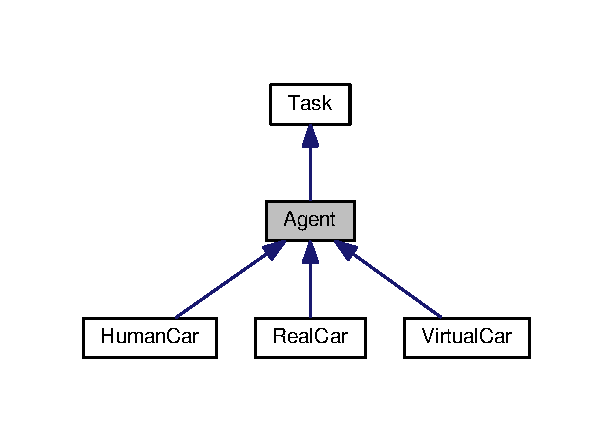
\includegraphics[width=294pt]{classAgent__inherit__graph}
\end{center}
\end{figure}


Collaboration diagram for Agent\+:\nopagebreak
\begin{figure}[H]
\begin{center}
\leavevmode
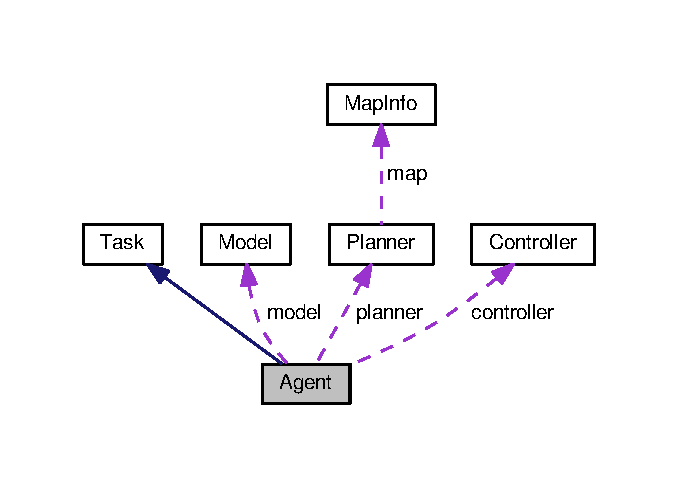
\includegraphics[width=326pt]{classAgent__coll__graph}
\end{center}
\end{figure}
\subsection*{Public Member Functions}
\begin{DoxyCompactItemize}
\item 
\hyperlink{classAgent_adaa4e2f9264e069d59ef234d26c8763e}{Agent} (int \hyperlink{classAgent_af8b58fe9dafe460ed2ddf87435a7feed}{id}, \hyperlink{Agent_8hpp_a5dd127bb3cb18b011cf5fd80a906e830}{Vector} initial\+State)
\item 
\hyperlink{classAgent_a7f32b3b61989f9dc8a3858bafff71da0}{Agent} (int \hyperlink{classAgent_af8b58fe9dafe460ed2ddf87435a7feed}{id}, \hyperlink{Agent_8hpp_a5dd127bb3cb18b011cf5fd80a906e830}{Vector} initial\+State, \hyperlink{classPlanner}{Planner} $\ast$\hyperlink{classAgent_aa71be9f465a3d8eed4e3297d8aa49eb1}{planner}, \hyperlink{classController}{Controller} $\ast$\hyperlink{classAgent_a35138f4fa7fa31760928b84680f7a886}{controller}, \hyperlink{classModel}{Model} $\ast$\hyperlink{classAgent_a41c7b65f7ad35cc6756cf0313edaa9a0}{model})
\item 
int \hyperlink{classAgent_aa5d95bd591e032b4763d9bbdf6ade810}{get\+Id} () const 
\item 
\hyperlink{Agent_8hpp_a5dd127bb3cb18b011cf5fd80a906e830}{Vector} \hyperlink{classAgent_a1661a5a75e7ab73c69269ed1270dc1e7}{get\+State} () const 
\item 
void \hyperlink{classAgent_aa204d1659d5057accf5ea283604eed2b}{set\+Next\+State} (\hyperlink{Agent_8hpp_a5dd127bb3cb18b011cf5fd80a906e830}{Vector} \hyperlink{classAgent_a6ef1b669e841f34e42619a2429160dc7}{state})
\item 
void \hyperlink{classAgent_a2e23f08188162e06a4072892d6919f9d}{apply\+Next\+State} ()
\begin{DoxyCompactList}\small\item\em Apply the next state which was previously set. \end{DoxyCompactList}\item 
void \hyperlink{classAgent_a917ab100e5e7ce4446269375869215b1}{set\+Planner} (\hyperlink{classPlanner}{Planner} $\ast$p)
\item 
void \hyperlink{classAgent_a5621b9471f9ed9bd8750709ff4fab46b}{set\+Controller} (\hyperlink{classController}{Controller} $\ast$c)
\item 
void \hyperlink{classAgent_a5a53cde60df6c2e733e809bdd1e96a56}{set\+Model} (\hyperlink{classModel}{Model} $\ast$m)
\item 
virtual \hyperlink{Agent_8hpp_ad2c3439c0fbb853c45129639d2581c51}{Agent\+Type} \hyperlink{classAgent_a48eedea220997f4aa85ce4596f2c49c5}{get\+Type} () const =0
\item 
void \hyperlink{classAgent_a80e144d0fd78f8e1a54abf92158448e1}{Run} ()
\begin{DoxyCompactList}\small\item\em Calculate next state via agent\textquotesingle{}s planner, controller and model. \end{DoxyCompactList}\end{DoxyCompactItemize}
\subsection*{Public Attributes}
\begin{DoxyCompactItemize}
\item 
int \hyperlink{classAgent_a7253eba145842d05f51375a1d8f7df91}{num} = 0
\end{DoxyCompactItemize}
\subsection*{Protected Attributes}
\begin{DoxyCompactItemize}
\item 
\hyperlink{Agent_8hpp_a5dd127bb3cb18b011cf5fd80a906e830}{Vector} \hyperlink{classAgent_a6ef1b669e841f34e42619a2429160dc7}{state}
\item 
const int \hyperlink{classAgent_aae845abfc5e48abee8efe8f1088ea5b4}{dim\+State}
\item 
const int \hyperlink{classAgent_af8b58fe9dafe460ed2ddf87435a7feed}{id}
\item 
\hyperlink{Agent_8hpp_a5dd127bb3cb18b011cf5fd80a906e830}{Vector} \hyperlink{classAgent_af6b03c80fd3fdc4bd34d3ca3027e67f2}{next\+State}
\item 
\hyperlink{classPlanner}{Planner} $\ast$ \hyperlink{classAgent_aa71be9f465a3d8eed4e3297d8aa49eb1}{planner}
\item 
\hyperlink{classController}{Controller} $\ast$ \hyperlink{classAgent_a35138f4fa7fa31760928b84680f7a886}{controller}
\item 
\hyperlink{classModel}{Model} $\ast$ \hyperlink{classAgent_a41c7b65f7ad35cc6756cf0313edaa9a0}{model}
\end{DoxyCompactItemize}
\subsection*{Friends}
\begin{DoxyCompactItemize}
\item 
bool \hyperlink{classAgent_ada5c7ad0216c88d7a21c2ae7825f2a81}{operator$<$} (\hyperlink{classAgent}{Agent} \&la, \hyperlink{classAgent}{Agent} \&ra)
\end{DoxyCompactItemize}


\subsection{Detailed Description}
The parent class of all agents. An agent has a state vector and an id. 

You can get the current state, or set the next state followed by applying the next state. 

\subsection{Constructor \& Destructor Documentation}
\index{Agent@{Agent}!Agent@{Agent}}
\index{Agent@{Agent}!Agent@{Agent}}
\subsubsection[{\texorpdfstring{Agent(int id, Vector initial\+State)}{Agent(int id, Vector initialState)}}]{\setlength{\rightskip}{0pt plus 5cm}Agent\+::\+Agent (
\begin{DoxyParamCaption}
\item[{int}]{id, }
\item[{{\bf Vector}}]{initial\+State}
\end{DoxyParamCaption}
)}\hypertarget{classAgent_adaa4e2f9264e069d59ef234d26c8763e}{}\label{classAgent_adaa4e2f9264e069d59ef234d26c8763e}
Constructor. 
\begin{DoxyParams}{Parameters}
{\em id} & the id of the agent. \\
\hline
{\em initial\+State} & the initial state of the agent. \\
\hline
\end{DoxyParams}
\index{Agent@{Agent}!Agent@{Agent}}
\index{Agent@{Agent}!Agent@{Agent}}
\subsubsection[{\texorpdfstring{Agent(int id, Vector initial\+State, Planner $\ast$planner, Controller $\ast$controller, Model $\ast$model)}{Agent(int id, Vector initialState, Planner *planner, Controller *controller, Model *model)}}]{\setlength{\rightskip}{0pt plus 5cm}Agent\+::\+Agent (
\begin{DoxyParamCaption}
\item[{int}]{id, }
\item[{{\bf Vector}}]{initial\+State, }
\item[{{\bf Planner} $\ast$}]{planner, }
\item[{{\bf Controller} $\ast$}]{controller, }
\item[{{\bf Model} $\ast$}]{model}
\end{DoxyParamCaption}
)\hspace{0.3cm}{\ttfamily [explicit]}}\hypertarget{classAgent_a7f32b3b61989f9dc8a3858bafff71da0}{}\label{classAgent_a7f32b3b61989f9dc8a3858bafff71da0}


\subsection{Member Function Documentation}
\index{Agent@{Agent}!apply\+Next\+State@{apply\+Next\+State}}
\index{apply\+Next\+State@{apply\+Next\+State}!Agent@{Agent}}
\subsubsection[{\texorpdfstring{apply\+Next\+State()}{applyNextState()}}]{\setlength{\rightskip}{0pt plus 5cm}void Agent\+::apply\+Next\+State (
\begin{DoxyParamCaption}
{}
\end{DoxyParamCaption}
)}\hypertarget{classAgent_a2e23f08188162e06a4072892d6919f9d}{}\label{classAgent_a2e23f08188162e06a4072892d6919f9d}


Apply the next state which was previously set. 

\index{Agent@{Agent}!get\+Id@{get\+Id}}
\index{get\+Id@{get\+Id}!Agent@{Agent}}
\subsubsection[{\texorpdfstring{get\+Id() const }{getId() const }}]{\setlength{\rightskip}{0pt plus 5cm}int Agent\+::get\+Id (
\begin{DoxyParamCaption}
{}
\end{DoxyParamCaption}
) const}\hypertarget{classAgent_aa5d95bd591e032b4763d9bbdf6ade810}{}\label{classAgent_aa5d95bd591e032b4763d9bbdf6ade810}
Get the agent id. \begin{DoxyReturn}{Returns}
agent id 
\end{DoxyReturn}
\index{Agent@{Agent}!get\+State@{get\+State}}
\index{get\+State@{get\+State}!Agent@{Agent}}
\subsubsection[{\texorpdfstring{get\+State() const }{getState() const }}]{\setlength{\rightskip}{0pt plus 5cm}{\bf Vector} Agent\+::get\+State (
\begin{DoxyParamCaption}
{}
\end{DoxyParamCaption}
) const}\hypertarget{classAgent_a1661a5a75e7ab73c69269ed1270dc1e7}{}\label{classAgent_a1661a5a75e7ab73c69269ed1270dc1e7}
Get the current state vector of the agent. \begin{DoxyReturn}{Returns}
current state. 
\end{DoxyReturn}
\index{Agent@{Agent}!get\+Type@{get\+Type}}
\index{get\+Type@{get\+Type}!Agent@{Agent}}
\subsubsection[{\texorpdfstring{get\+Type() const =0}{getType() const =0}}]{\setlength{\rightskip}{0pt plus 5cm}virtual {\bf Agent\+Type} Agent\+::get\+Type (
\begin{DoxyParamCaption}
{}
\end{DoxyParamCaption}
) const\hspace{0.3cm}{\ttfamily [pure virtual]}}\hypertarget{classAgent_a48eedea220997f4aa85ce4596f2c49c5}{}\label{classAgent_a48eedea220997f4aa85ce4596f2c49c5}


Implemented in \hyperlink{classHumanCar_af824211de46d6c802e17d8b04e4dae33}{Human\+Car}, \hyperlink{classRealCar_ab77ba7bc138ad5d1676a0562d44017f7}{Real\+Car}, and \hyperlink{classVirtualCar_a642228555a81aef7d410b162b0437cf2}{Virtual\+Car}.

\index{Agent@{Agent}!Run@{Run}}
\index{Run@{Run}!Agent@{Agent}}
\subsubsection[{\texorpdfstring{Run()}{Run()}}]{\setlength{\rightskip}{0pt plus 5cm}void Agent\+::\+Run (
\begin{DoxyParamCaption}
{}
\end{DoxyParamCaption}
)\hspace{0.3cm}{\ttfamily [virtual]}}\hypertarget{classAgent_a80e144d0fd78f8e1a54abf92158448e1}{}\label{classAgent_a80e144d0fd78f8e1a54abf92158448e1}


Calculate next state via agent\textquotesingle{}s planner, controller and model. 



Reimplemented from \hyperlink{classTask_a18ea998d77c751e6e1581f7035022a5b}{Task}.

\index{Agent@{Agent}!set\+Controller@{set\+Controller}}
\index{set\+Controller@{set\+Controller}!Agent@{Agent}}
\subsubsection[{\texorpdfstring{set\+Controller(\+Controller $\ast$c)}{setController(Controller *c)}}]{\setlength{\rightskip}{0pt plus 5cm}void Agent\+::set\+Controller (
\begin{DoxyParamCaption}
\item[{{\bf Controller} $\ast$}]{c}
\end{DoxyParamCaption}
)}\hypertarget{classAgent_a5621b9471f9ed9bd8750709ff4fab46b}{}\label{classAgent_a5621b9471f9ed9bd8750709ff4fab46b}

\begin{DoxyParams}{Parameters}
{\em c} & the controller that will be set to the agent \\
\hline
\end{DoxyParams}
\index{Agent@{Agent}!set\+Model@{set\+Model}}
\index{set\+Model@{set\+Model}!Agent@{Agent}}
\subsubsection[{\texorpdfstring{set\+Model(\+Model $\ast$m)}{setModel(Model *m)}}]{\setlength{\rightskip}{0pt plus 5cm}void Agent\+::set\+Model (
\begin{DoxyParamCaption}
\item[{{\bf Model} $\ast$}]{m}
\end{DoxyParamCaption}
)}\hypertarget{classAgent_a5a53cde60df6c2e733e809bdd1e96a56}{}\label{classAgent_a5a53cde60df6c2e733e809bdd1e96a56}

\begin{DoxyParams}{Parameters}
{\em m} & the model that will be set to the agent \\
\hline
\end{DoxyParams}
\index{Agent@{Agent}!set\+Next\+State@{set\+Next\+State}}
\index{set\+Next\+State@{set\+Next\+State}!Agent@{Agent}}
\subsubsection[{\texorpdfstring{set\+Next\+State(\+Vector state)}{setNextState(Vector state)}}]{\setlength{\rightskip}{0pt plus 5cm}void Agent\+::set\+Next\+State (
\begin{DoxyParamCaption}
\item[{{\bf Vector}}]{state}
\end{DoxyParamCaption}
)}\hypertarget{classAgent_aa204d1659d5057accf5ea283604eed2b}{}\label{classAgent_aa204d1659d5057accf5ea283604eed2b}
Set the next state vector of the agent. 
\begin{DoxyParams}{Parameters}
{\em state} & next state to set (but not applied immediately) \\
\hline
\end{DoxyParams}
\index{Agent@{Agent}!set\+Planner@{set\+Planner}}
\index{set\+Planner@{set\+Planner}!Agent@{Agent}}
\subsubsection[{\texorpdfstring{set\+Planner(\+Planner $\ast$p)}{setPlanner(Planner *p)}}]{\setlength{\rightskip}{0pt plus 5cm}void Agent\+::set\+Planner (
\begin{DoxyParamCaption}
\item[{{\bf Planner} $\ast$}]{p}
\end{DoxyParamCaption}
)}\hypertarget{classAgent_a917ab100e5e7ce4446269375869215b1}{}\label{classAgent_a917ab100e5e7ce4446269375869215b1}

\begin{DoxyParams}{Parameters}
{\em p} & the planner that will be set to the agent \\
\hline
\end{DoxyParams}


\subsection{Friends And Related Function Documentation}
\index{Agent@{Agent}!operator$<$@{operator$<$}}
\index{operator$<$@{operator$<$}!Agent@{Agent}}
\subsubsection[{\texorpdfstring{operator$<$}{operator<}}]{\setlength{\rightskip}{0pt plus 5cm}bool operator$<$ (
\begin{DoxyParamCaption}
\item[{{\bf Agent} \&}]{la, }
\item[{{\bf Agent} \&}]{ra}
\end{DoxyParamCaption}
)\hspace{0.3cm}{\ttfamily [friend]}}\hypertarget{classAgent_ada5c7ad0216c88d7a21c2ae7825f2a81}{}\label{classAgent_ada5c7ad0216c88d7a21c2ae7825f2a81}


\subsection{Member Data Documentation}
\index{Agent@{Agent}!controller@{controller}}
\index{controller@{controller}!Agent@{Agent}}
\subsubsection[{\texorpdfstring{controller}{controller}}]{\setlength{\rightskip}{0pt plus 5cm}{\bf Controller}$\ast$ Agent\+::controller\hspace{0.3cm}{\ttfamily [protected]}}\hypertarget{classAgent_a35138f4fa7fa31760928b84680f7a886}{}\label{classAgent_a35138f4fa7fa31760928b84680f7a886}
the agent\textquotesingle{}s \hyperlink{classController}{Controller} \index{Agent@{Agent}!dim\+State@{dim\+State}}
\index{dim\+State@{dim\+State}!Agent@{Agent}}
\subsubsection[{\texorpdfstring{dim\+State}{dimState}}]{\setlength{\rightskip}{0pt plus 5cm}const int Agent\+::dim\+State\hspace{0.3cm}{\ttfamily [protected]}}\hypertarget{classAgent_aae845abfc5e48abee8efe8f1088ea5b4}{}\label{classAgent_aae845abfc5e48abee8efe8f1088ea5b4}
the dimension of the agent state \index{Agent@{Agent}!id@{id}}
\index{id@{id}!Agent@{Agent}}
\subsubsection[{\texorpdfstring{id}{id}}]{\setlength{\rightskip}{0pt plus 5cm}const int Agent\+::id\hspace{0.3cm}{\ttfamily [protected]}}\hypertarget{classAgent_af8b58fe9dafe460ed2ddf87435a7feed}{}\label{classAgent_af8b58fe9dafe460ed2ddf87435a7feed}
the agent\textquotesingle{}s ID \index{Agent@{Agent}!model@{model}}
\index{model@{model}!Agent@{Agent}}
\subsubsection[{\texorpdfstring{model}{model}}]{\setlength{\rightskip}{0pt plus 5cm}{\bf Model}$\ast$ Agent\+::model\hspace{0.3cm}{\ttfamily [protected]}}\hypertarget{classAgent_a41c7b65f7ad35cc6756cf0313edaa9a0}{}\label{classAgent_a41c7b65f7ad35cc6756cf0313edaa9a0}
the agent\textquotesingle{}s \hyperlink{classModel}{Model} \index{Agent@{Agent}!next\+State@{next\+State}}
\index{next\+State@{next\+State}!Agent@{Agent}}
\subsubsection[{\texorpdfstring{next\+State}{nextState}}]{\setlength{\rightskip}{0pt plus 5cm}{\bf Vector} Agent\+::next\+State\hspace{0.3cm}{\ttfamily [protected]}}\hypertarget{classAgent_af6b03c80fd3fdc4bd34d3ca3027e67f2}{}\label{classAgent_af6b03c80fd3fdc4bd34d3ca3027e67f2}
next state which is calculated from model and waiting for apply \index{Agent@{Agent}!num@{num}}
\index{num@{num}!Agent@{Agent}}
\subsubsection[{\texorpdfstring{num}{num}}]{\setlength{\rightskip}{0pt plus 5cm}int Agent\+::num = 0}\hypertarget{classAgent_a7253eba145842d05f51375a1d8f7df91}{}\label{classAgent_a7253eba145842d05f51375a1d8f7df91}
\index{Agent@{Agent}!planner@{planner}}
\index{planner@{planner}!Agent@{Agent}}
\subsubsection[{\texorpdfstring{planner}{planner}}]{\setlength{\rightskip}{0pt plus 5cm}{\bf Planner}$\ast$ Agent\+::planner\hspace{0.3cm}{\ttfamily [protected]}}\hypertarget{classAgent_aa71be9f465a3d8eed4e3297d8aa49eb1}{}\label{classAgent_aa71be9f465a3d8eed4e3297d8aa49eb1}
the agent\textquotesingle{}s \hyperlink{classPlanner}{Planner} \index{Agent@{Agent}!state@{state}}
\index{state@{state}!Agent@{Agent}}
\subsubsection[{\texorpdfstring{state}{state}}]{\setlength{\rightskip}{0pt plus 5cm}{\bf Vector} Agent\+::state\hspace{0.3cm}{\ttfamily [protected]}}\hypertarget{classAgent_a6ef1b669e841f34e42619a2429160dc7}{}\label{classAgent_a6ef1b669e841f34e42619a2429160dc7}
the current state of the agent 

The documentation for this class was generated from the following files\+:\begin{DoxyCompactItemize}
\item 
Agents/\hyperlink{Agent_8hpp}{Agent.\+hpp}\item 
Agents/\hyperlink{Agent_8cpp}{Agent.\+cpp}\end{DoxyCompactItemize}

\hypertarget{classBusyThreadContainer}{}\section{Busy\+Thread\+Container Class Reference}
\label{classBusyThreadContainer}\index{Busy\+Thread\+Container@{Busy\+Thread\+Container}}


The class of busy thread container.  




{\ttfamily \#include $<$Busy\+Thread\+Container.\+hpp$>$}

\subsection*{Public Member Functions}
\begin{DoxyCompactItemize}
\item 
\hyperlink{classBusyThreadContainer_a77719862a87674e9b7f012d3f3aceac2}{Busy\+Thread\+Container} ()
\item 
\hyperlink{classBusyThreadContainer_ab71b388d1a6ecf1d0c977ebce7fa3f3a}{$\sim$\+Busy\+Thread\+Container} ()
\item 
void \hyperlink{classBusyThreadContainer_a601b1d5736511f3d07ed506b179c9433}{push} (\hyperlink{classMyThread}{My\+Thread} $\ast$m)
\begin{DoxyCompactList}\small\item\em Push a thread into the busy thread container. \end{DoxyCompactList}\item 
std\+::list$<$ \hyperlink{classMyThread}{My\+Thread} $\ast$ $>$\+::size\+\_\+type \hyperlink{classBusyThreadContainer_ab84986bf500d5e527b022a75be74d0f6}{size} ()
\begin{DoxyCompactList}\small\item\em Get the size of the busy thread container. \end{DoxyCompactList}\item 
void \hyperlink{classBusyThreadContainer_aacfa7ece73b73ef5036f49979f4412e9}{erase} (\hyperlink{classMyThread}{My\+Thread} $\ast$m)
\begin{DoxyCompactList}\small\item\em Erase a thread from the busy thread container. \end{DoxyCompactList}\end{DoxyCompactItemize}
\subsection*{Private Types}
\begin{DoxyCompactItemize}
\item 
typedef std\+::list$<$ \hyperlink{classMyThread}{My\+Thread} $\ast$ $>$ \hyperlink{classBusyThreadContainer_ab3e046394f1969fb1f43ea358c1c6950}{Container}
\item 
typedef Container\+::iterator \hyperlink{classBusyThreadContainer_acc7f249156d5ed707acefe652f07fb18}{Iterator}
\end{DoxyCompactItemize}
\subsection*{Private Attributes}
\begin{DoxyCompactItemize}
\item 
std\+::list$<$ \hyperlink{classMyThread}{My\+Thread} $\ast$ $>$ \hyperlink{classBusyThreadContainer_a8dc554b281ea8fdd9faf24166de0d4d3}{busy\+\_\+thread\+\_\+container\+\_\+}
\end{DoxyCompactItemize}


\subsection{Detailed Description}
The class of busy thread container. 

It contains threads which is in using 

\subsection{Member Typedef Documentation}
\index{Busy\+Thread\+Container@{Busy\+Thread\+Container}!Container@{Container}}
\index{Container@{Container}!Busy\+Thread\+Container@{Busy\+Thread\+Container}}
\subsubsection[{\texorpdfstring{Container}{Container}}]{\setlength{\rightskip}{0pt plus 5cm}typedef std\+::list$<${\bf My\+Thread}$\ast$$>$ {\bf Busy\+Thread\+Container\+::\+Container}\hspace{0.3cm}{\ttfamily [private]}}\hypertarget{classBusyThreadContainer_ab3e046394f1969fb1f43ea358c1c6950}{}\label{classBusyThreadContainer_ab3e046394f1969fb1f43ea358c1c6950}
\index{Busy\+Thread\+Container@{Busy\+Thread\+Container}!Iterator@{Iterator}}
\index{Iterator@{Iterator}!Busy\+Thread\+Container@{Busy\+Thread\+Container}}
\subsubsection[{\texorpdfstring{Iterator}{Iterator}}]{\setlength{\rightskip}{0pt plus 5cm}typedef Container\+::iterator {\bf Busy\+Thread\+Container\+::\+Iterator}\hspace{0.3cm}{\ttfamily [private]}}\hypertarget{classBusyThreadContainer_acc7f249156d5ed707acefe652f07fb18}{}\label{classBusyThreadContainer_acc7f249156d5ed707acefe652f07fb18}


\subsection{Constructor \& Destructor Documentation}
\index{Busy\+Thread\+Container@{Busy\+Thread\+Container}!Busy\+Thread\+Container@{Busy\+Thread\+Container}}
\index{Busy\+Thread\+Container@{Busy\+Thread\+Container}!Busy\+Thread\+Container@{Busy\+Thread\+Container}}
\subsubsection[{\texorpdfstring{Busy\+Thread\+Container()}{BusyThreadContainer()}}]{\setlength{\rightskip}{0pt plus 5cm}Busy\+Thread\+Container\+::\+Busy\+Thread\+Container (
\begin{DoxyParamCaption}
{}
\end{DoxyParamCaption}
)}\hypertarget{classBusyThreadContainer_a77719862a87674e9b7f012d3f3aceac2}{}\label{classBusyThreadContainer_a77719862a87674e9b7f012d3f3aceac2}
\index{Busy\+Thread\+Container@{Busy\+Thread\+Container}!````~Busy\+Thread\+Container@{$\sim$\+Busy\+Thread\+Container}}
\index{````~Busy\+Thread\+Container@{$\sim$\+Busy\+Thread\+Container}!Busy\+Thread\+Container@{Busy\+Thread\+Container}}
\subsubsection[{\texorpdfstring{$\sim$\+Busy\+Thread\+Container()}{~BusyThreadContainer()}}]{\setlength{\rightskip}{0pt plus 5cm}Busy\+Thread\+Container\+::$\sim$\+Busy\+Thread\+Container (
\begin{DoxyParamCaption}
{}
\end{DoxyParamCaption}
)}\hypertarget{classBusyThreadContainer_ab71b388d1a6ecf1d0c977ebce7fa3f3a}{}\label{classBusyThreadContainer_ab71b388d1a6ecf1d0c977ebce7fa3f3a}


\subsection{Member Function Documentation}
\index{Busy\+Thread\+Container@{Busy\+Thread\+Container}!erase@{erase}}
\index{erase@{erase}!Busy\+Thread\+Container@{Busy\+Thread\+Container}}
\subsubsection[{\texorpdfstring{erase(\+My\+Thread $\ast$m)}{erase(MyThread *m)}}]{\setlength{\rightskip}{0pt plus 5cm}void Busy\+Thread\+Container\+::erase (
\begin{DoxyParamCaption}
\item[{{\bf My\+Thread} $\ast$}]{m}
\end{DoxyParamCaption}
)}\hypertarget{classBusyThreadContainer_aacfa7ece73b73ef5036f49979f4412e9}{}\label{classBusyThreadContainer_aacfa7ece73b73ef5036f49979f4412e9}


Erase a thread from the busy thread container. 

\index{Busy\+Thread\+Container@{Busy\+Thread\+Container}!push@{push}}
\index{push@{push}!Busy\+Thread\+Container@{Busy\+Thread\+Container}}
\subsubsection[{\texorpdfstring{push(\+My\+Thread $\ast$m)}{push(MyThread *m)}}]{\setlength{\rightskip}{0pt plus 5cm}void Busy\+Thread\+Container\+::push (
\begin{DoxyParamCaption}
\item[{{\bf My\+Thread} $\ast$}]{m}
\end{DoxyParamCaption}
)}\hypertarget{classBusyThreadContainer_a601b1d5736511f3d07ed506b179c9433}{}\label{classBusyThreadContainer_a601b1d5736511f3d07ed506b179c9433}


Push a thread into the busy thread container. 

\index{Busy\+Thread\+Container@{Busy\+Thread\+Container}!size@{size}}
\index{size@{size}!Busy\+Thread\+Container@{Busy\+Thread\+Container}}
\subsubsection[{\texorpdfstring{size()}{size()}}]{\setlength{\rightskip}{0pt plus 5cm}std\+::list$<$ {\bf My\+Thread} $\ast$ $>$\+::size\+\_\+type Busy\+Thread\+Container\+::size (
\begin{DoxyParamCaption}
{}
\end{DoxyParamCaption}
)}\hypertarget{classBusyThreadContainer_ab84986bf500d5e527b022a75be74d0f6}{}\label{classBusyThreadContainer_ab84986bf500d5e527b022a75be74d0f6}


Get the size of the busy thread container. 



\subsection{Member Data Documentation}
\index{Busy\+Thread\+Container@{Busy\+Thread\+Container}!busy\+\_\+thread\+\_\+container\+\_\+@{busy\+\_\+thread\+\_\+container\+\_\+}}
\index{busy\+\_\+thread\+\_\+container\+\_\+@{busy\+\_\+thread\+\_\+container\+\_\+}!Busy\+Thread\+Container@{Busy\+Thread\+Container}}
\subsubsection[{\texorpdfstring{busy\+\_\+thread\+\_\+container\+\_\+}{busy_thread_container_}}]{\setlength{\rightskip}{0pt plus 5cm}std\+::list$<${\bf My\+Thread}$\ast$$>$ Busy\+Thread\+Container\+::busy\+\_\+thread\+\_\+container\+\_\+\hspace{0.3cm}{\ttfamily [private]}}\hypertarget{classBusyThreadContainer_a8dc554b281ea8fdd9faf24166de0d4d3}{}\label{classBusyThreadContainer_a8dc554b281ea8fdd9faf24166de0d4d3}
The busy thread container itself 

The documentation for this class was generated from the following files\+:\begin{DoxyCompactItemize}
\item 
thread\+Pool/\hyperlink{BusyThreadContainer_8hpp}{Busy\+Thread\+Container.\+hpp}\item 
thread\+Pool/\hyperlink{BusyThreadContainer_8cpp}{Busy\+Thread\+Container.\+cpp}\end{DoxyCompactItemize}

\hypertarget{classController}{}\section{Controller Class Reference}
\label{classController}\index{Controller@{Controller}}


Parent class of all controllers.  




{\ttfamily \#include $<$Controller.\+hpp$>$}



Inheritance diagram for Controller\+:\nopagebreak
\begin{figure}[H]
\begin{center}
\leavevmode
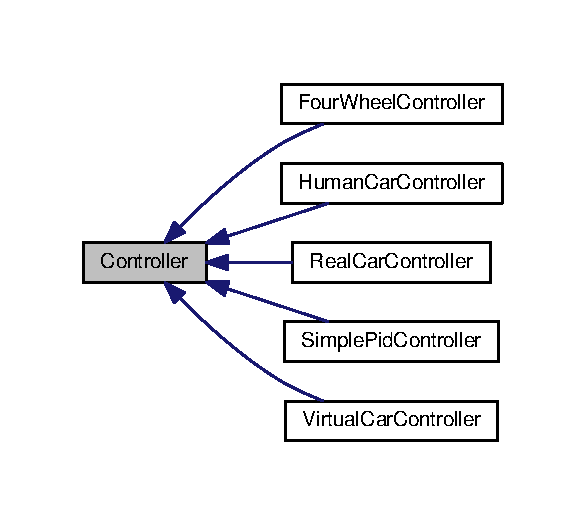
\includegraphics[width=281pt]{classController__inherit__graph}
\end{center}
\end{figure}
\subsection*{Public Member Functions}
\begin{DoxyCompactItemize}
\item 
\hyperlink{classController_aad5cc1765e936fb123c5cb90f120e415}{Controller} (int \hyperlink{classController_a187167b349efb6c61871efd990824219}{dim\+Input}, int \hyperlink{classController_a6d34c8bf130f8b8631117ca3e8b44a5d}{dim\+Intermediate})
\item 
virtual \hyperlink{Agent_8hpp_a5dd127bb3cb18b011cf5fd80a906e830}{Vector} \hyperlink{classController_acef11e408fb0d66d272bf5ab828cfbf6}{update} (\hyperlink{Agent_8hpp_a5dd127bb3cb18b011cf5fd80a906e830}{Vector} input)=0
\end{DoxyCompactItemize}
\subsection*{Protected Attributes}
\begin{DoxyCompactItemize}
\item 
const int \hyperlink{classController_a187167b349efb6c61871efd990824219}{dim\+Input}
\item 
const int \hyperlink{classController_a6d34c8bf130f8b8631117ca3e8b44a5d}{dim\+Intermediate}
\end{DoxyCompactItemize}


\subsection{Detailed Description}
Parent class of all controllers. 

\subsection{Constructor \& Destructor Documentation}
\index{Controller@{Controller}!Controller@{Controller}}
\index{Controller@{Controller}!Controller@{Controller}}
\subsubsection[{\texorpdfstring{Controller(int dim\+Input, int dim\+Intermediate)}{Controller(int dimInput, int dimIntermediate)}}]{\setlength{\rightskip}{0pt plus 5cm}Controller\+::\+Controller (
\begin{DoxyParamCaption}
\item[{int}]{dim\+Input, }
\item[{int}]{dim\+Intermediate}
\end{DoxyParamCaption}
)\hspace{0.3cm}{\ttfamily [explicit]}}\hypertarget{classController_aad5cc1765e936fb123c5cb90f120e415}{}\label{classController_aad5cc1765e936fb123c5cb90f120e415}
Constructor. 
\begin{DoxyParams}{Parameters}
{\em dim\+Input} & dimension of the input vector, which is constant for a certain type of controllers. \\
\hline
{\em dim\+Intermediate} & dimension of the intermediate vector, which is constant for a certain type of controllers. \\
\hline
\end{DoxyParams}


\subsection{Member Function Documentation}
\index{Controller@{Controller}!update@{update}}
\index{update@{update}!Controller@{Controller}}
\subsubsection[{\texorpdfstring{update(\+Vector input)=0}{update(Vector input)=0}}]{\setlength{\rightskip}{0pt plus 5cm}virtual {\bf Vector} Controller\+::update (
\begin{DoxyParamCaption}
\item[{{\bf Vector}}]{input}
\end{DoxyParamCaption}
)\hspace{0.3cm}{\ttfamily [pure virtual]}}\hypertarget{classController_acef11e408fb0d66d272bf5ab828cfbf6}{}\label{classController_acef11e408fb0d66d272bf5ab828cfbf6}


Implemented in \hyperlink{classSimplePidController_ae849967e635ea1c6237f614d08156931}{Simple\+Pid\+Controller}, \hyperlink{classFourWheelController_a2db0c3dac61cec36963c9b1c9c7ddeef}{Four\+Wheel\+Controller}, \hyperlink{classHumanCarController_aa20daebb65f2e2111f5d7af09b81d886}{Human\+Car\+Controller}, \hyperlink{classRealCarController_a639c0c911bbfc63ce90f9de2b8a9be4d}{Real\+Car\+Controller}, and \hyperlink{classVirtualCarController_acab2f4c5b7e8ef7ed5013058e6871fff}{Virtual\+Car\+Controller}.



\subsection{Member Data Documentation}
\index{Controller@{Controller}!dim\+Input@{dim\+Input}}
\index{dim\+Input@{dim\+Input}!Controller@{Controller}}
\subsubsection[{\texorpdfstring{dim\+Input}{dimInput}}]{\setlength{\rightskip}{0pt plus 5cm}const int Controller\+::dim\+Input\hspace{0.3cm}{\ttfamily [protected]}}\hypertarget{classController_a187167b349efb6c61871efd990824219}{}\label{classController_a187167b349efb6c61871efd990824219}
dimension of the input vector. \index{Controller@{Controller}!dim\+Intermediate@{dim\+Intermediate}}
\index{dim\+Intermediate@{dim\+Intermediate}!Controller@{Controller}}
\subsubsection[{\texorpdfstring{dim\+Intermediate}{dimIntermediate}}]{\setlength{\rightskip}{0pt plus 5cm}const int Controller\+::dim\+Intermediate\hspace{0.3cm}{\ttfamily [protected]}}\hypertarget{classController_a6d34c8bf130f8b8631117ca3e8b44a5d}{}\label{classController_a6d34c8bf130f8b8631117ca3e8b44a5d}
dimension of the intermediate vector. 

The documentation for this class was generated from the following files\+:\begin{DoxyCompactItemize}
\item 
Controllers/\hyperlink{Controller_8hpp}{Controller.\+hpp}\item 
Controllers/\hyperlink{Controller_8cpp}{Controller.\+cpp}\end{DoxyCompactItemize}

\hypertarget{classFourWheelController}{}\section{Four\+Wheel\+Controller Class Reference}
\label{classFourWheelController}\index{Four\+Wheel\+Controller@{Four\+Wheel\+Controller}}


A four-\/wheel controller is the controller for the complex car model (\hyperlink{classFourWheelModel}{Four\+Wheel\+Model})  




{\ttfamily \#include $<$Four\+Wheel\+Controller.\+hpp$>$}



Inheritance diagram for Four\+Wheel\+Controller\+:\nopagebreak
\begin{figure}[H]
\begin{center}
\leavevmode
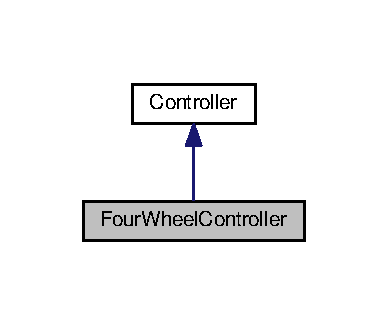
\includegraphics[width=186pt]{classFourWheelController__inherit__graph}
\end{center}
\end{figure}


Collaboration diagram for Four\+Wheel\+Controller\+:\nopagebreak
\begin{figure}[H]
\begin{center}
\leavevmode
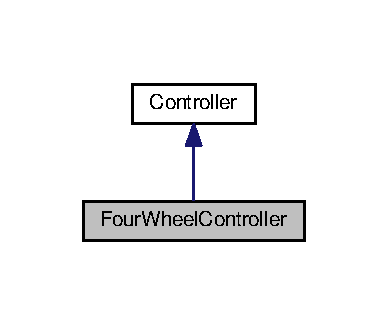
\includegraphics[width=186pt]{classFourWheelController__coll__graph}
\end{center}
\end{figure}
\subsection*{Public Member Functions}
\begin{DoxyCompactItemize}
\item 
\hyperlink{classFourWheelController_ada2276db9e38f1cdfd2506988b5ca5bb}{Four\+Wheel\+Controller} ()
\item 
\hyperlink{Agent_8hpp_a5dd127bb3cb18b011cf5fd80a906e830}{Vector} \hyperlink{classFourWheelController_a2db0c3dac61cec36963c9b1c9c7ddeef}{update} (\hyperlink{Agent_8hpp_a5dd127bb3cb18b011cf5fd80a906e830}{Vector} input) override
\end{DoxyCompactItemize}
\subsection*{Additional Inherited Members}


\subsection{Detailed Description}
A four-\/wheel controller is the controller for the complex car model (\hyperlink{classFourWheelModel}{Four\+Wheel\+Model}) 

\subsection{Constructor \& Destructor Documentation}
\index{Four\+Wheel\+Controller@{Four\+Wheel\+Controller}!Four\+Wheel\+Controller@{Four\+Wheel\+Controller}}
\index{Four\+Wheel\+Controller@{Four\+Wheel\+Controller}!Four\+Wheel\+Controller@{Four\+Wheel\+Controller}}
\subsubsection[{\texorpdfstring{Four\+Wheel\+Controller()}{FourWheelController()}}]{\setlength{\rightskip}{0pt plus 5cm}Four\+Wheel\+Controller\+::\+Four\+Wheel\+Controller (
\begin{DoxyParamCaption}
{}
\end{DoxyParamCaption}
)\hspace{0.3cm}{\ttfamily [explicit]}}\hypertarget{classFourWheelController_ada2276db9e38f1cdfd2506988b5ca5bb}{}\label{classFourWheelController_ada2276db9e38f1cdfd2506988b5ca5bb}
Constructor. Dimension of input vector is 3 (gas pedal, brake pedal, steering angle) Dimension of intermediate vector is 3. 

\subsection{Member Function Documentation}
\index{Four\+Wheel\+Controller@{Four\+Wheel\+Controller}!update@{update}}
\index{update@{update}!Four\+Wheel\+Controller@{Four\+Wheel\+Controller}}
\subsubsection[{\texorpdfstring{update(\+Vector input) override}{update(Vector input) override}}]{\setlength{\rightskip}{0pt plus 5cm}{\bf Vector} Four\+Wheel\+Controller\+::update (
\begin{DoxyParamCaption}
\item[{{\bf Vector}}]{input}
\end{DoxyParamCaption}
)\hspace{0.3cm}{\ttfamily [override]}, {\ttfamily [virtual]}}\hypertarget{classFourWheelController_a2db0c3dac61cec36963c9b1c9c7ddeef}{}\label{classFourWheelController_a2db0c3dac61cec36963c9b1c9c7ddeef}
Proportional controller. 
\begin{DoxyParams}{Parameters}
{\em input} & input vector (gas pedal, brake pedal, steering angle) \\
\hline
\end{DoxyParams}
\begin{DoxyReturn}{Returns}
intermediate vector. 
\end{DoxyReturn}


Implements \hyperlink{classController_acef11e408fb0d66d272bf5ab828cfbf6}{Controller}.



The documentation for this class was generated from the following files\+:\begin{DoxyCompactItemize}
\item 
Controllers/\hyperlink{FourWheelController_8hpp}{Four\+Wheel\+Controller.\+hpp}\item 
Controllers/\hyperlink{FourWheelController_8cpp}{Four\+Wheel\+Controller.\+cpp}\end{DoxyCompactItemize}

\hypertarget{classFourWheelModel}{}\section{Four\+Wheel\+Model Class Reference}
\label{classFourWheelModel}\index{Four\+Wheel\+Model@{Four\+Wheel\+Model}}


Complex model for a human car.  




{\ttfamily \#include $<$Four\+Wheel\+Model.\+hpp$>$}



Inheritance diagram for Four\+Wheel\+Model\+:\nopagebreak
\begin{figure}[H]
\begin{center}
\leavevmode
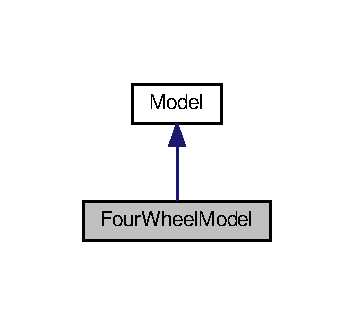
\includegraphics[width=170pt]{classFourWheelModel__inherit__graph}
\end{center}
\end{figure}


Collaboration diagram for Four\+Wheel\+Model\+:\nopagebreak
\begin{figure}[H]
\begin{center}
\leavevmode
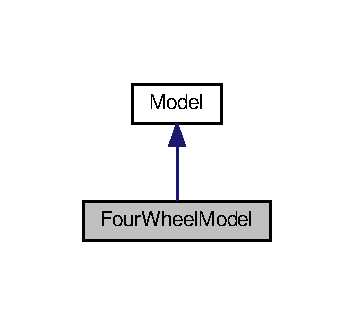
\includegraphics[width=170pt]{classFourWheelModel__coll__graph}
\end{center}
\end{figure}
\subsection*{Public Member Functions}
\begin{DoxyCompactItemize}
\item 
\hyperlink{classFourWheelModel_a2ae886651e6494e9655cdfe7bb55523f}{Four\+Wheel\+Model} ()
\item 
virtual \hyperlink{classFourWheelModel_a58298c9fc4880ff13b4f2f7271536c77}{$\sim$\+Four\+Wheel\+Model} ()
\item 
\hyperlink{Agent_8hpp_a5dd127bb3cb18b011cf5fd80a906e830}{Vector} \hyperlink{classFourWheelModel_a2169e82abcb344e4bb345c563e6ea7de}{update} (\hyperlink{Agent_8hpp_a5dd127bb3cb18b011cf5fd80a906e830}{Vector} state, \hyperlink{Agent_8hpp_a5dd127bb3cb18b011cf5fd80a906e830}{Vector} intermediate) override
\end{DoxyCompactItemize}
\subsection*{Private Attributes}
\begin{DoxyCompactItemize}
\item 
Car\+\_\+4wheel $\ast$ \hyperlink{classFourWheelModel_aa4e5165e690a959eda31d186f83e615d}{inner\+Model}
\item 
long int \hyperlink{classFourWheelModel_a56bbb1ac91d8c35a239776d6beb49109}{count}
\end{DoxyCompactItemize}
\subsection*{Additional Inherited Members}


\subsection{Detailed Description}
Complex model for a human car. 

\subsection{Constructor \& Destructor Documentation}
\index{Four\+Wheel\+Model@{Four\+Wheel\+Model}!Four\+Wheel\+Model@{Four\+Wheel\+Model}}
\index{Four\+Wheel\+Model@{Four\+Wheel\+Model}!Four\+Wheel\+Model@{Four\+Wheel\+Model}}
\subsubsection[{\texorpdfstring{Four\+Wheel\+Model()}{FourWheelModel()}}]{\setlength{\rightskip}{0pt plus 5cm}Four\+Wheel\+Model\+::\+Four\+Wheel\+Model (
\begin{DoxyParamCaption}
{}
\end{DoxyParamCaption}
)\hspace{0.3cm}{\ttfamily [explicit]}}\hypertarget{classFourWheelModel_a2ae886651e6494e9655cdfe7bb55523f}{}\label{classFourWheelModel_a2ae886651e6494e9655cdfe7bb55523f}
Constructor. Dimension of state vector is 6 (x, y, yaw, speed x, speed y, speed yaw) Dimension of intermediate vector is 3 (proportional to gas pedal, brake pedal, and steering angle) \index{Four\+Wheel\+Model@{Four\+Wheel\+Model}!````~Four\+Wheel\+Model@{$\sim$\+Four\+Wheel\+Model}}
\index{````~Four\+Wheel\+Model@{$\sim$\+Four\+Wheel\+Model}!Four\+Wheel\+Model@{Four\+Wheel\+Model}}
\subsubsection[{\texorpdfstring{$\sim$\+Four\+Wheel\+Model()}{~FourWheelModel()}}]{\setlength{\rightskip}{0pt plus 5cm}Four\+Wheel\+Model\+::$\sim$\+Four\+Wheel\+Model (
\begin{DoxyParamCaption}
{}
\end{DoxyParamCaption}
)\hspace{0.3cm}{\ttfamily [virtual]}}\hypertarget{classFourWheelModel_a58298c9fc4880ff13b4f2f7271536c77}{}\label{classFourWheelModel_a58298c9fc4880ff13b4f2f7271536c77}


\subsection{Member Function Documentation}
\index{Four\+Wheel\+Model@{Four\+Wheel\+Model}!update@{update}}
\index{update@{update}!Four\+Wheel\+Model@{Four\+Wheel\+Model}}
\subsubsection[{\texorpdfstring{update(\+Vector state, Vector intermediate) override}{update(Vector state, Vector intermediate) override}}]{\setlength{\rightskip}{0pt plus 5cm}{\bf Vector} Four\+Wheel\+Model\+::update (
\begin{DoxyParamCaption}
\item[{{\bf Vector}}]{state, }
\item[{{\bf Vector}}]{intermediate}
\end{DoxyParamCaption}
)\hspace{0.3cm}{\ttfamily [override]}, {\ttfamily [virtual]}}\hypertarget{classFourWheelModel_a2169e82abcb344e4bb345c563e6ea7de}{}\label{classFourWheelModel_a2169e82abcb344e4bb345c563e6ea7de}
Wrapper for the complex model 
\begin{DoxyParams}{Parameters}
{\em state} & Dimension of state vector is 6 (x, y, yaw, speed x, speed y, speed yaw) \\
\hline
{\em intermediate} & Dimension of intermediate vector is 3 (proportional to gas pedal, brake pedal, and steering angle) \\
\hline
\end{DoxyParams}
\begin{DoxyReturn}{Returns}
the state vector of this car for the next iteration 
\end{DoxyReturn}


Implements \hyperlink{classModel_a887e642d0c195b771af8300c7c817f09}{Model}.



\subsection{Member Data Documentation}
\index{Four\+Wheel\+Model@{Four\+Wheel\+Model}!count@{count}}
\index{count@{count}!Four\+Wheel\+Model@{Four\+Wheel\+Model}}
\subsubsection[{\texorpdfstring{count}{count}}]{\setlength{\rightskip}{0pt plus 5cm}long int Four\+Wheel\+Model\+::count\hspace{0.3cm}{\ttfamily [private]}}\hypertarget{classFourWheelModel_a56bbb1ac91d8c35a239776d6beb49109}{}\label{classFourWheelModel_a56bbb1ac91d8c35a239776d6beb49109}
\index{Four\+Wheel\+Model@{Four\+Wheel\+Model}!inner\+Model@{inner\+Model}}
\index{inner\+Model@{inner\+Model}!Four\+Wheel\+Model@{Four\+Wheel\+Model}}
\subsubsection[{\texorpdfstring{inner\+Model}{innerModel}}]{\setlength{\rightskip}{0pt plus 5cm}Car\+\_\+4wheel$\ast$ Four\+Wheel\+Model\+::inner\+Model\hspace{0.3cm}{\ttfamily [private]}}\hypertarget{classFourWheelModel_aa4e5165e690a959eda31d186f83e615d}{}\label{classFourWheelModel_aa4e5165e690a959eda31d186f83e615d}


The documentation for this class was generated from the following files\+:\begin{DoxyCompactItemize}
\item 
Models/\hyperlink{FourWheelModel_8hpp}{Four\+Wheel\+Model.\+hpp}\item 
Models/\hyperlink{FourWheelModel_8cpp}{Four\+Wheel\+Model.\+cpp}\end{DoxyCompactItemize}

\hypertarget{classHumanCar}{}\section{Human\+Car Class Reference}
\label{classHumanCar}\index{Human\+Car@{Human\+Car}}


{\ttfamily \#include $<$Human\+Car.\+hpp$>$}



Inheritance diagram for Human\+Car\+:\nopagebreak
\begin{figure}[H]
\begin{center}
\leavevmode
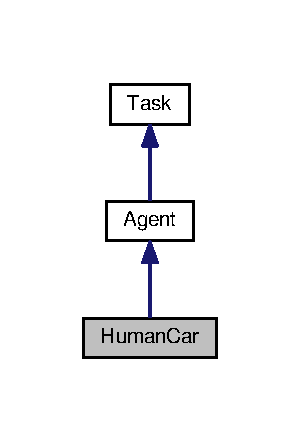
\includegraphics[width=144pt]{classHumanCar__inherit__graph}
\end{center}
\end{figure}


Collaboration diagram for Human\+Car\+:\nopagebreak
\begin{figure}[H]
\begin{center}
\leavevmode
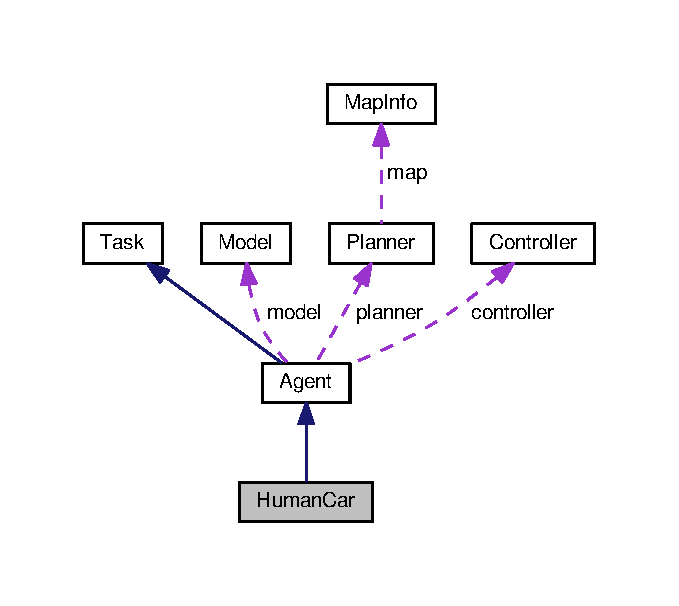
\includegraphics[width=326pt]{classHumanCar__coll__graph}
\end{center}
\end{figure}
\subsection*{Public Member Functions}
\begin{DoxyCompactItemize}
\item 
\hyperlink{classHumanCar_aa7ff47db66e59687205e2339936e3933}{Human\+Car} (int \hyperlink{classAgent_af8b58fe9dafe460ed2ddf87435a7feed}{id}, \hyperlink{Agent_8hpp_a5dd127bb3cb18b011cf5fd80a906e830}{Vector} initial\+State)
\item 
\hyperlink{classHumanCar_a9372d14b0cc0018c79def3f80f0fea3c}{Human\+Car} (int \hyperlink{classAgent_af8b58fe9dafe460ed2ddf87435a7feed}{id}, \hyperlink{Agent_8hpp_a5dd127bb3cb18b011cf5fd80a906e830}{Vector} initial\+State, \hyperlink{classPlanner}{Planner} $\ast$\hyperlink{classAgent_aa71be9f465a3d8eed4e3297d8aa49eb1}{planner}, \hyperlink{classController}{Controller} $\ast$\hyperlink{classAgent_a35138f4fa7fa31760928b84680f7a886}{controller}, \hyperlink{classModel}{Model} $\ast$\hyperlink{classAgent_a41c7b65f7ad35cc6756cf0313edaa9a0}{model})
\item 
\hyperlink{Agent_8hpp_ad2c3439c0fbb853c45129639d2581c51}{Agent\+Type} \hyperlink{classHumanCar_af824211de46d6c802e17d8b04e4dae33}{get\+Type} () const override
\end{DoxyCompactItemize}
\subsection*{Additional Inherited Members}


\subsection{Detailed Description}
\hyperlink{classHumanCar}{Human\+Car} is a kind of agent that is controlled by humans. It is the \char`\"{}car\char`\"{} put in the lab. It doesn\textquotesingle{}t move in the real world 

\subsection{Constructor \& Destructor Documentation}
\index{Human\+Car@{Human\+Car}!Human\+Car@{Human\+Car}}
\index{Human\+Car@{Human\+Car}!Human\+Car@{Human\+Car}}
\subsubsection[{\texorpdfstring{Human\+Car(int id, Vector initial\+State)}{HumanCar(int id, Vector initialState)}}]{\setlength{\rightskip}{0pt plus 5cm}Human\+Car\+::\+Human\+Car (
\begin{DoxyParamCaption}
\item[{int}]{id, }
\item[{{\bf Vector}}]{initial\+State}
\end{DoxyParamCaption}
)}\hypertarget{classHumanCar_aa7ff47db66e59687205e2339936e3933}{}\label{classHumanCar_aa7ff47db66e59687205e2339936e3933}
\index{Human\+Car@{Human\+Car}!Human\+Car@{Human\+Car}}
\index{Human\+Car@{Human\+Car}!Human\+Car@{Human\+Car}}
\subsubsection[{\texorpdfstring{Human\+Car(int id, Vector initial\+State, Planner $\ast$planner, Controller $\ast$controller, Model $\ast$model)}{HumanCar(int id, Vector initialState, Planner *planner, Controller *controller, Model *model)}}]{\setlength{\rightskip}{0pt plus 5cm}Human\+Car\+::\+Human\+Car (
\begin{DoxyParamCaption}
\item[{int}]{id, }
\item[{{\bf Vector}}]{initial\+State, }
\item[{{\bf Planner} $\ast$}]{planner, }
\item[{{\bf Controller} $\ast$}]{controller, }
\item[{{\bf Model} $\ast$}]{model}
\end{DoxyParamCaption}
)\hspace{0.3cm}{\ttfamily [explicit]}}\hypertarget{classHumanCar_a9372d14b0cc0018c79def3f80f0fea3c}{}\label{classHumanCar_a9372d14b0cc0018c79def3f80f0fea3c}
Constructor. 
\begin{DoxyParams}{Parameters}
{\em id} & id of the new human car. \\
\hline
{\em initial\+State} & initial state of the human car. \\
\hline
\end{DoxyParams}


\subsection{Member Function Documentation}
\index{Human\+Car@{Human\+Car}!get\+Type@{get\+Type}}
\index{get\+Type@{get\+Type}!Human\+Car@{Human\+Car}}
\subsubsection[{\texorpdfstring{get\+Type() const override}{getType() const override}}]{\setlength{\rightskip}{0pt plus 5cm}{\bf Agent\+Type} Human\+Car\+::get\+Type (
\begin{DoxyParamCaption}
{}
\end{DoxyParamCaption}
) const\hspace{0.3cm}{\ttfamily [override]}, {\ttfamily [virtual]}}\hypertarget{classHumanCar_af824211de46d6c802e17d8b04e4dae33}{}\label{classHumanCar_af824211de46d6c802e17d8b04e4dae33}
Type getter (overridden) \begin{DoxyReturn}{Returns}
type (human car) 
\end{DoxyReturn}


Implements \hyperlink{classAgent_a48eedea220997f4aa85ce4596f2c49c5}{Agent}.



The documentation for this class was generated from the following files\+:\begin{DoxyCompactItemize}
\item 
Agents/\hyperlink{HumanCar_8hpp}{Human\+Car.\+hpp}\item 
Agents/\hyperlink{HumanCar_8cpp}{Human\+Car.\+cpp}\end{DoxyCompactItemize}

\hypertarget{classHumanCarController}{}\section{Human\+Car\+Controller Class Reference}
\label{classHumanCarController}\index{Human\+Car\+Controller@{Human\+Car\+Controller}}


A human car controller is the controller for the kinematic car model (\hyperlink{classHumanCarModel}{Human\+Car\+Model})  




{\ttfamily \#include $<$Human\+Car\+Controller.\+hpp$>$}



Inheritance diagram for Human\+Car\+Controller\+:\nopagebreak
\begin{figure}[H]
\begin{center}
\leavevmode
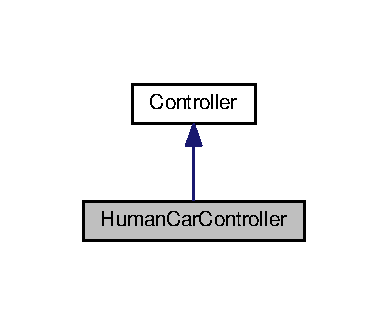
\includegraphics[width=186pt]{classHumanCarController__inherit__graph}
\end{center}
\end{figure}


Collaboration diagram for Human\+Car\+Controller\+:\nopagebreak
\begin{figure}[H]
\begin{center}
\leavevmode
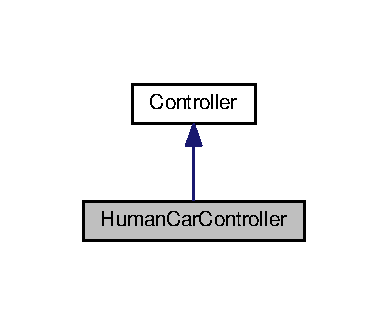
\includegraphics[width=186pt]{classHumanCarController__coll__graph}
\end{center}
\end{figure}
\subsection*{Public Member Functions}
\begin{DoxyCompactItemize}
\item 
\hyperlink{classHumanCarController_a34efd6c56d364c6a55056ee37136da4b}{Human\+Car\+Controller} ()
\item 
\hyperlink{Agent_8hpp_a5dd127bb3cb18b011cf5fd80a906e830}{Vector} \hyperlink{classHumanCarController_aa20daebb65f2e2111f5d7af09b81d886}{update} (\hyperlink{Agent_8hpp_a5dd127bb3cb18b011cf5fd80a906e830}{Vector} input) override
\end{DoxyCompactItemize}
\subsection*{Additional Inherited Members}


\subsection{Detailed Description}
A human car controller is the controller for the kinematic car model (\hyperlink{classHumanCarModel}{Human\+Car\+Model}) 

\subsection{Constructor \& Destructor Documentation}
\index{Human\+Car\+Controller@{Human\+Car\+Controller}!Human\+Car\+Controller@{Human\+Car\+Controller}}
\index{Human\+Car\+Controller@{Human\+Car\+Controller}!Human\+Car\+Controller@{Human\+Car\+Controller}}
\subsubsection[{\texorpdfstring{Human\+Car\+Controller()}{HumanCarController()}}]{\setlength{\rightskip}{0pt plus 5cm}Human\+Car\+Controller\+::\+Human\+Car\+Controller (
\begin{DoxyParamCaption}
{}
\end{DoxyParamCaption}
)\hspace{0.3cm}{\ttfamily [explicit]}}\hypertarget{classHumanCarController_a34efd6c56d364c6a55056ee37136da4b}{}\label{classHumanCarController_a34efd6c56d364c6a55056ee37136da4b}
Constructor. Dimension of input vector is 3 (gas pedal, brake pedal, steering angle) Dimension of intermediate vector is 3. 

\subsection{Member Function Documentation}
\index{Human\+Car\+Controller@{Human\+Car\+Controller}!update@{update}}
\index{update@{update}!Human\+Car\+Controller@{Human\+Car\+Controller}}
\subsubsection[{\texorpdfstring{update(\+Vector input) override}{update(Vector input) override}}]{\setlength{\rightskip}{0pt plus 5cm}{\bf Vector} Human\+Car\+Controller\+::update (
\begin{DoxyParamCaption}
\item[{{\bf Vector}}]{input}
\end{DoxyParamCaption}
)\hspace{0.3cm}{\ttfamily [override]}, {\ttfamily [virtual]}}\hypertarget{classHumanCarController_aa20daebb65f2e2111f5d7af09b81d886}{}\label{classHumanCarController_aa20daebb65f2e2111f5d7af09b81d886}
Proportional controller. 
\begin{DoxyParams}{Parameters}
{\em input} & input vector (gas pedal, brake pedal, steering angle) \\
\hline
\end{DoxyParams}
\begin{DoxyReturn}{Returns}
intermediate vector. 
\end{DoxyReturn}


Implements \hyperlink{classController_acef11e408fb0d66d272bf5ab828cfbf6}{Controller}.



The documentation for this class was generated from the following files\+:\begin{DoxyCompactItemize}
\item 
Controllers/\hyperlink{HumanCarController_8hpp}{Human\+Car\+Controller.\+hpp}\item 
Controllers/\hyperlink{HumanCarController_8cpp}{Human\+Car\+Controller.\+cpp}\end{DoxyCompactItemize}

\hypertarget{classHumanCarModel}{}\section{Human\+Car\+Model Class Reference}
\label{classHumanCarModel}\index{Human\+Car\+Model@{Human\+Car\+Model}}


Simple kinematic model for a human car.  




{\ttfamily \#include $<$Human\+Car\+Model.\+hpp$>$}



Inheritance diagram for Human\+Car\+Model\+:\nopagebreak
\begin{figure}[H]
\begin{center}
\leavevmode
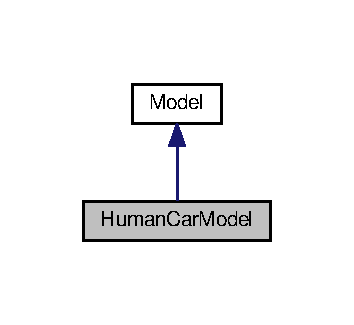
\includegraphics[width=170pt]{classHumanCarModel__inherit__graph}
\end{center}
\end{figure}


Collaboration diagram for Human\+Car\+Model\+:\nopagebreak
\begin{figure}[H]
\begin{center}
\leavevmode
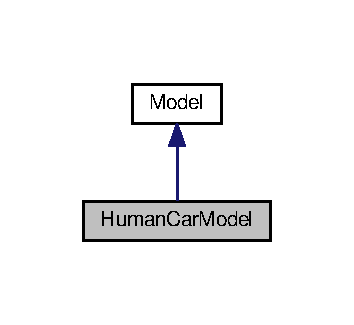
\includegraphics[width=170pt]{classHumanCarModel__coll__graph}
\end{center}
\end{figure}
\subsection*{Public Member Functions}
\begin{DoxyCompactItemize}
\item 
\hyperlink{classHumanCarModel_a50fe8a46cefbbdc0feaedae39947da50}{Human\+Car\+Model} ()
\item 
\hyperlink{Agent_8hpp_a5dd127bb3cb18b011cf5fd80a906e830}{Vector} \hyperlink{classHumanCarModel_aeaa782fab7b9ea5d9b245df0ced2b7cb}{update} (\hyperlink{Agent_8hpp_a5dd127bb3cb18b011cf5fd80a906e830}{Vector} state, \hyperlink{Agent_8hpp_a5dd127bb3cb18b011cf5fd80a906e830}{Vector} intermediate) override
\end{DoxyCompactItemize}
\subsection*{Additional Inherited Members}


\subsection{Detailed Description}
Simple kinematic model for a human car. 

\subsection{Constructor \& Destructor Documentation}
\index{Human\+Car\+Model@{Human\+Car\+Model}!Human\+Car\+Model@{Human\+Car\+Model}}
\index{Human\+Car\+Model@{Human\+Car\+Model}!Human\+Car\+Model@{Human\+Car\+Model}}
\subsubsection[{\texorpdfstring{Human\+Car\+Model()}{HumanCarModel()}}]{\setlength{\rightskip}{0pt plus 5cm}Human\+Car\+Model\+::\+Human\+Car\+Model (
\begin{DoxyParamCaption}
{}
\end{DoxyParamCaption}
)\hspace{0.3cm}{\ttfamily [explicit]}}\hypertarget{classHumanCarModel_a50fe8a46cefbbdc0feaedae39947da50}{}\label{classHumanCarModel_a50fe8a46cefbbdc0feaedae39947da50}
Constructor. Dimension of state vector is 6 (x, y, yaw, speed x, speed y, speed yaw) Dimension of intermediate vector is 3 (proportional to gas pedal, brake pedal, and steering angle) 

\subsection{Member Function Documentation}
\index{Human\+Car\+Model@{Human\+Car\+Model}!update@{update}}
\index{update@{update}!Human\+Car\+Model@{Human\+Car\+Model}}
\subsubsection[{\texorpdfstring{update(\+Vector state, Vector intermediate) override}{update(Vector state, Vector intermediate) override}}]{\setlength{\rightskip}{0pt plus 5cm}{\bf Vector} Human\+Car\+Model\+::update (
\begin{DoxyParamCaption}
\item[{{\bf Vector}}]{state, }
\item[{{\bf Vector}}]{intermediate}
\end{DoxyParamCaption}
)\hspace{0.3cm}{\ttfamily [override]}, {\ttfamily [virtual]}}\hypertarget{classHumanCarModel_aeaa782fab7b9ea5d9b245df0ced2b7cb}{}\label{classHumanCarModel_aeaa782fab7b9ea5d9b245df0ced2b7cb}
Implements the simple kinematic model 
\begin{DoxyParams}{Parameters}
{\em state} & Dimension of state vector is 6 (x, y, yaw, speed x, speed y, speed yaw) \\
\hline
{\em intermediate} & Dimension of intermediate vector is 3 (proportional to gas pedal, brake pedal, and steering angle) \\
\hline
\end{DoxyParams}
\begin{DoxyReturn}{Returns}
the state vector of this car for the next iteration 
\end{DoxyReturn}


Implements \hyperlink{classModel_a887e642d0c195b771af8300c7c817f09}{Model}.



The documentation for this class was generated from the following files\+:\begin{DoxyCompactItemize}
\item 
Models/\hyperlink{HumanCarModel_8hpp}{Human\+Car\+Model.\+hpp}\item 
Models/\hyperlink{HumanCarModel_8cpp}{Human\+Car\+Model.\+cpp}\end{DoxyCompactItemize}

\hypertarget{classHumanCarPlanner}{}\section{Human\+Car\+Planner Class Reference}
\label{classHumanCarPlanner}\index{Human\+Car\+Planner@{Human\+Car\+Planner}}


\hyperlink{classPlanner}{Planner} for a human car, which passes human inputs directly.  




{\ttfamily \#include $<$Human\+Car\+Planner.\+hpp$>$}



Inheritance diagram for Human\+Car\+Planner\+:\nopagebreak
\begin{figure}[H]
\begin{center}
\leavevmode
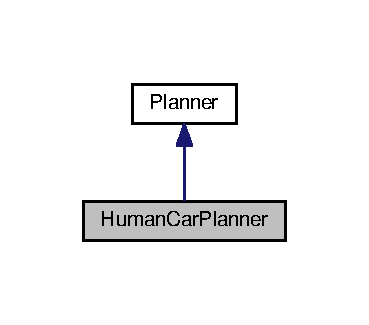
\includegraphics[width=177pt]{classHumanCarPlanner__inherit__graph}
\end{center}
\end{figure}


Collaboration diagram for Human\+Car\+Planner\+:\nopagebreak
\begin{figure}[H]
\begin{center}
\leavevmode
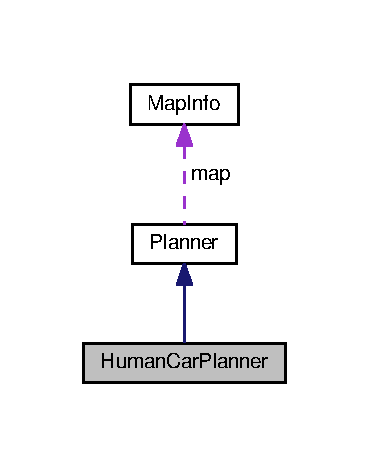
\includegraphics[width=177pt]{classHumanCarPlanner__coll__graph}
\end{center}
\end{figure}
\subsection*{Public Member Functions}
\begin{DoxyCompactItemize}
\item 
\hyperlink{classHumanCarPlanner_afde9292f62bb4fb8172719a1cd74e09a}{Human\+Car\+Planner} ()
\item 
\hyperlink{Agent_8hpp_a5dd127bb3cb18b011cf5fd80a906e830}{Vector} \hyperlink{classHumanCarPlanner_ad6c513730ee6374f64d1cf5cdb842af1}{update} (\hyperlink{Agent_8hpp_a5dd127bb3cb18b011cf5fd80a906e830}{Vector} current\+State, const \hyperlink{Agent_8hpp_a5dd127bb3cb18b011cf5fd80a906e830}{Vector} \&human\+Input, std\+::vector$<$ \hyperlink{classAgent}{Agent} $\ast$ $>$ agents) override
\end{DoxyCompactItemize}
\subsection*{Additional Inherited Members}


\subsection{Detailed Description}
\hyperlink{classPlanner}{Planner} for a human car, which passes human inputs directly. 

\subsection{Constructor \& Destructor Documentation}
\index{Human\+Car\+Planner@{Human\+Car\+Planner}!Human\+Car\+Planner@{Human\+Car\+Planner}}
\index{Human\+Car\+Planner@{Human\+Car\+Planner}!Human\+Car\+Planner@{Human\+Car\+Planner}}
\subsubsection[{\texorpdfstring{Human\+Car\+Planner()}{HumanCarPlanner()}}]{\setlength{\rightskip}{0pt plus 5cm}Human\+Car\+Planner\+::\+Human\+Car\+Planner (
\begin{DoxyParamCaption}
{}
\end{DoxyParamCaption}
)\hspace{0.3cm}{\ttfamily [explicit]}}\hypertarget{classHumanCarPlanner_afde9292f62bb4fb8172719a1cd74e09a}{}\label{classHumanCarPlanner_afde9292f62bb4fb8172719a1cd74e09a}
Constructor. Dimension of state vector is 6 (x, y, yaw, speed x, speed y, speed yaw) Dimension of input vector is 3 (gas pedal, brake pedal, and steering angle) 

\subsection{Member Function Documentation}
\index{Human\+Car\+Planner@{Human\+Car\+Planner}!update@{update}}
\index{update@{update}!Human\+Car\+Planner@{Human\+Car\+Planner}}
\subsubsection[{\texorpdfstring{update(\+Vector current\+State, const Vector \&human\+Input, std\+::vector$<$ Agent $\ast$ $>$ agents) override}{update(Vector currentState, const Vector &humanInput, std::vector< Agent * > agents) override}}]{\setlength{\rightskip}{0pt plus 5cm}{\bf Vector} Human\+Car\+Planner\+::update (
\begin{DoxyParamCaption}
\item[{{\bf Vector}}]{current\+State, }
\item[{const {\bf Vector} \&}]{human\+Input, }
\item[{std\+::vector$<$ {\bf Agent} $\ast$ $>$}]{agents}
\end{DoxyParamCaption}
)\hspace{0.3cm}{\ttfamily [override]}, {\ttfamily [virtual]}}\hypertarget{classHumanCarPlanner_ad6c513730ee6374f64d1cf5cdb842af1}{}\label{classHumanCarPlanner_ad6c513730ee6374f64d1cf5cdb842af1}
\hyperlink{classPlanner}{Planner} for a human car\+: Pass the human input directly 
\begin{DoxyParams}{Parameters}
{\em current\+State} & current state of the car \\
\hline
{\em human\+Input} & current human input vector (gas pedal, brake pedal, and steering angle) \\
\hline
{\em agents} & information of all agents in the simulator. \\
\hline
\end{DoxyParams}
\begin{DoxyReturn}{Returns}
input vector (human input) 
\end{DoxyReturn}


Implements \hyperlink{classPlanner_a62e1434402a3f36b0883e069a10447d8}{Planner}.



The documentation for this class was generated from the following files\+:\begin{DoxyCompactItemize}
\item 
Planners/\hyperlink{HumanCarPlanner_8hpp}{Human\+Car\+Planner.\+hpp}\item 
Planners/\hyperlink{HumanCarPlanner_8cpp}{Human\+Car\+Planner.\+cpp}\end{DoxyCompactItemize}

\hypertarget{classIdleThreadContainer}{}\section{Idle\+Thread\+Container Class Reference}
\label{classIdleThreadContainer}\index{Idle\+Thread\+Container@{Idle\+Thread\+Container}}


The class of idle thread container.  




{\ttfamily \#include $<$Idle\+Thread\+Container.\+hpp$>$}

\subsection*{Public Member Functions}
\begin{DoxyCompactItemize}
\item 
\hyperlink{classIdleThreadContainer_a83d8818aa23117b2988cf5983196aff7}{Idle\+Thread\+Container} ()
\item 
\hyperlink{classIdleThreadContainer_a62e8c40ae681cc19c8a77c5905e63b91}{$\sim$\+Idle\+Thread\+Container} ()
\item 
std\+::vector$<$ \hyperlink{classMyThread}{My\+Thread} $\ast$ $>$\+::size\+\_\+type \hyperlink{classIdleThreadContainer_a5b1b0dbbcd69816ed8f4a9b117428536}{size} ()
\begin{DoxyCompactList}\small\item\em Get the size of the idle thread container. \end{DoxyCompactList}\item 
void \hyperlink{classIdleThreadContainer_a3874126045ab92244f7489439f9a28ee}{push} (\hyperlink{classMyThread}{My\+Thread} $\ast$m)
\begin{DoxyCompactList}\small\item\em Push a thread into the idle thread container. \end{DoxyCompactList}\item 
void \hyperlink{classIdleThreadContainer_a4165535fed8aa4c36b9327b9c58d951b}{assign} (int n, \hyperlink{classMyThreadPool}{My\+Thread\+Pool} $\ast$m)
\begin{DoxyCompactList}\small\item\em Assign a thread into the idle thread container of a thread pool. \end{DoxyCompactList}\item 
\hyperlink{classMyThread}{My\+Thread} $\ast$ \hyperlink{classIdleThreadContainer_a8df6ccc5fb9d17e47cfd74e75ab1af96}{top} ()
\begin{DoxyCompactList}\small\item\em Get the last thread from the idle thread container. \end{DoxyCompactList}\item 
void \hyperlink{classIdleThreadContainer_a1debcb3e02119e266a8f1c641ba458c2}{pop} ()
\begin{DoxyCompactList}\small\item\em Get the last thread from the idle thread container. \end{DoxyCompactList}\item 
void \hyperlink{classIdleThreadContainer_a16a7d9ff37543470418fe401a9260594}{erase} (\hyperlink{classMyThread}{My\+Thread} $\ast$m)
\begin{DoxyCompactList}\small\item\em Erase a thread from the idle thread container. \end{DoxyCompactList}\end{DoxyCompactItemize}
\subsection*{Private Types}
\begin{DoxyCompactItemize}
\item 
typedef std\+::vector$<$ \hyperlink{classMyThread}{My\+Thread} $\ast$ $>$ \hyperlink{classIdleThreadContainer_a640f978c12404f8c82fc6052b3f7ef12}{Container}
\item 
typedef Container\+::iterator \hyperlink{classIdleThreadContainer_a5e29f54ae2f9d426521ed58c06794cf7}{Iterator}
\end{DoxyCompactItemize}
\subsection*{Private Attributes}
\begin{DoxyCompactItemize}
\item 
std\+::vector$<$ \hyperlink{classMyThread}{My\+Thread} $\ast$ $>$ \hyperlink{classIdleThreadContainer_a9ae4221b817dbdaa014c88e9eef3f9da}{idle\+\_\+thread\+\_\+container\+\_\+}
\end{DoxyCompactItemize}


\subsection{Detailed Description}
The class of idle thread container. 

It contains threads which is not in using 

\subsection{Member Typedef Documentation}
\index{Idle\+Thread\+Container@{Idle\+Thread\+Container}!Container@{Container}}
\index{Container@{Container}!Idle\+Thread\+Container@{Idle\+Thread\+Container}}
\subsubsection[{\texorpdfstring{Container}{Container}}]{\setlength{\rightskip}{0pt plus 5cm}typedef std\+::vector$<${\bf My\+Thread}$\ast$$>$ {\bf Idle\+Thread\+Container\+::\+Container}\hspace{0.3cm}{\ttfamily [private]}}\hypertarget{classIdleThreadContainer_a640f978c12404f8c82fc6052b3f7ef12}{}\label{classIdleThreadContainer_a640f978c12404f8c82fc6052b3f7ef12}
\index{Idle\+Thread\+Container@{Idle\+Thread\+Container}!Iterator@{Iterator}}
\index{Iterator@{Iterator}!Idle\+Thread\+Container@{Idle\+Thread\+Container}}
\subsubsection[{\texorpdfstring{Iterator}{Iterator}}]{\setlength{\rightskip}{0pt plus 5cm}typedef Container\+::iterator {\bf Idle\+Thread\+Container\+::\+Iterator}\hspace{0.3cm}{\ttfamily [private]}}\hypertarget{classIdleThreadContainer_a5e29f54ae2f9d426521ed58c06794cf7}{}\label{classIdleThreadContainer_a5e29f54ae2f9d426521ed58c06794cf7}


\subsection{Constructor \& Destructor Documentation}
\index{Idle\+Thread\+Container@{Idle\+Thread\+Container}!Idle\+Thread\+Container@{Idle\+Thread\+Container}}
\index{Idle\+Thread\+Container@{Idle\+Thread\+Container}!Idle\+Thread\+Container@{Idle\+Thread\+Container}}
\subsubsection[{\texorpdfstring{Idle\+Thread\+Container()}{IdleThreadContainer()}}]{\setlength{\rightskip}{0pt plus 5cm}Idle\+Thread\+Container\+::\+Idle\+Thread\+Container (
\begin{DoxyParamCaption}
{}
\end{DoxyParamCaption}
)}\hypertarget{classIdleThreadContainer_a83d8818aa23117b2988cf5983196aff7}{}\label{classIdleThreadContainer_a83d8818aa23117b2988cf5983196aff7}
\index{Idle\+Thread\+Container@{Idle\+Thread\+Container}!````~Idle\+Thread\+Container@{$\sim$\+Idle\+Thread\+Container}}
\index{````~Idle\+Thread\+Container@{$\sim$\+Idle\+Thread\+Container}!Idle\+Thread\+Container@{Idle\+Thread\+Container}}
\subsubsection[{\texorpdfstring{$\sim$\+Idle\+Thread\+Container()}{~IdleThreadContainer()}}]{\setlength{\rightskip}{0pt plus 5cm}Idle\+Thread\+Container\+::$\sim$\+Idle\+Thread\+Container (
\begin{DoxyParamCaption}
{}
\end{DoxyParamCaption}
)}\hypertarget{classIdleThreadContainer_a62e8c40ae681cc19c8a77c5905e63b91}{}\label{classIdleThreadContainer_a62e8c40ae681cc19c8a77c5905e63b91}


\subsection{Member Function Documentation}
\index{Idle\+Thread\+Container@{Idle\+Thread\+Container}!assign@{assign}}
\index{assign@{assign}!Idle\+Thread\+Container@{Idle\+Thread\+Container}}
\subsubsection[{\texorpdfstring{assign(int n, My\+Thread\+Pool $\ast$m)}{assign(int n, MyThreadPool *m)}}]{\setlength{\rightskip}{0pt plus 5cm}void Idle\+Thread\+Container\+::assign (
\begin{DoxyParamCaption}
\item[{int}]{n, }
\item[{{\bf My\+Thread\+Pool} $\ast$}]{m}
\end{DoxyParamCaption}
)}\hypertarget{classIdleThreadContainer_a4165535fed8aa4c36b9327b9c58d951b}{}\label{classIdleThreadContainer_a4165535fed8aa4c36b9327b9c58d951b}


Assign a thread into the idle thread container of a thread pool. 

\index{Idle\+Thread\+Container@{Idle\+Thread\+Container}!erase@{erase}}
\index{erase@{erase}!Idle\+Thread\+Container@{Idle\+Thread\+Container}}
\subsubsection[{\texorpdfstring{erase(\+My\+Thread $\ast$m)}{erase(MyThread *m)}}]{\setlength{\rightskip}{0pt plus 5cm}void Idle\+Thread\+Container\+::erase (
\begin{DoxyParamCaption}
\item[{{\bf My\+Thread} $\ast$}]{m}
\end{DoxyParamCaption}
)}\hypertarget{classIdleThreadContainer_a16a7d9ff37543470418fe401a9260594}{}\label{classIdleThreadContainer_a16a7d9ff37543470418fe401a9260594}


Erase a thread from the idle thread container. 

\index{Idle\+Thread\+Container@{Idle\+Thread\+Container}!pop@{pop}}
\index{pop@{pop}!Idle\+Thread\+Container@{Idle\+Thread\+Container}}
\subsubsection[{\texorpdfstring{pop()}{pop()}}]{\setlength{\rightskip}{0pt plus 5cm}void Idle\+Thread\+Container\+::pop (
\begin{DoxyParamCaption}
{}
\end{DoxyParamCaption}
)}\hypertarget{classIdleThreadContainer_a1debcb3e02119e266a8f1c641ba458c2}{}\label{classIdleThreadContainer_a1debcb3e02119e266a8f1c641ba458c2}


Get the last thread from the idle thread container. 

\index{Idle\+Thread\+Container@{Idle\+Thread\+Container}!push@{push}}
\index{push@{push}!Idle\+Thread\+Container@{Idle\+Thread\+Container}}
\subsubsection[{\texorpdfstring{push(\+My\+Thread $\ast$m)}{push(MyThread *m)}}]{\setlength{\rightskip}{0pt plus 5cm}void Idle\+Thread\+Container\+::push (
\begin{DoxyParamCaption}
\item[{{\bf My\+Thread} $\ast$}]{m}
\end{DoxyParamCaption}
)}\hypertarget{classIdleThreadContainer_a3874126045ab92244f7489439f9a28ee}{}\label{classIdleThreadContainer_a3874126045ab92244f7489439f9a28ee}


Push a thread into the idle thread container. 

\index{Idle\+Thread\+Container@{Idle\+Thread\+Container}!size@{size}}
\index{size@{size}!Idle\+Thread\+Container@{Idle\+Thread\+Container}}
\subsubsection[{\texorpdfstring{size()}{size()}}]{\setlength{\rightskip}{0pt plus 5cm}std\+::vector$<$ {\bf My\+Thread} $\ast$ $>$\+::size\+\_\+type Idle\+Thread\+Container\+::size (
\begin{DoxyParamCaption}
{}
\end{DoxyParamCaption}
)}\hypertarget{classIdleThreadContainer_a5b1b0dbbcd69816ed8f4a9b117428536}{}\label{classIdleThreadContainer_a5b1b0dbbcd69816ed8f4a9b117428536}


Get the size of the idle thread container. 

\index{Idle\+Thread\+Container@{Idle\+Thread\+Container}!top@{top}}
\index{top@{top}!Idle\+Thread\+Container@{Idle\+Thread\+Container}}
\subsubsection[{\texorpdfstring{top()}{top()}}]{\setlength{\rightskip}{0pt plus 5cm}{\bf My\+Thread} $\ast$ Idle\+Thread\+Container\+::top (
\begin{DoxyParamCaption}
{}
\end{DoxyParamCaption}
)}\hypertarget{classIdleThreadContainer_a8df6ccc5fb9d17e47cfd74e75ab1af96}{}\label{classIdleThreadContainer_a8df6ccc5fb9d17e47cfd74e75ab1af96}


Get the last thread from the idle thread container. 



\subsection{Member Data Documentation}
\index{Idle\+Thread\+Container@{Idle\+Thread\+Container}!idle\+\_\+thread\+\_\+container\+\_\+@{idle\+\_\+thread\+\_\+container\+\_\+}}
\index{idle\+\_\+thread\+\_\+container\+\_\+@{idle\+\_\+thread\+\_\+container\+\_\+}!Idle\+Thread\+Container@{Idle\+Thread\+Container}}
\subsubsection[{\texorpdfstring{idle\+\_\+thread\+\_\+container\+\_\+}{idle_thread_container_}}]{\setlength{\rightskip}{0pt plus 5cm}std\+::vector$<${\bf My\+Thread}$\ast$$>$ Idle\+Thread\+Container\+::idle\+\_\+thread\+\_\+container\+\_\+\hspace{0.3cm}{\ttfamily [private]}}\hypertarget{classIdleThreadContainer_a9ae4221b817dbdaa014c88e9eef3f9da}{}\label{classIdleThreadContainer_a9ae4221b817dbdaa014c88e9eef3f9da}
The idle thread container itself 

The documentation for this class was generated from the following files\+:\begin{DoxyCompactItemize}
\item 
thread\+Pool/\hyperlink{IdleThreadContainer_8hpp}{Idle\+Thread\+Container.\+hpp}\item 
thread\+Pool/\hyperlink{IdleThreadContainer_8cpp}{Idle\+Thread\+Container.\+cpp}\end{DoxyCompactItemize}

\hypertarget{classMapInfo}{}\section{Map\+Info Class Reference}
\label{classMapInfo}\index{Map\+Info@{Map\+Info}}


this class is for read map. For now it is empty.  




{\ttfamily \#include $<$Map\+Info.\+hpp$>$}



\subsection{Detailed Description}
this class is for read map. For now it is empty. 

The documentation for this class was generated from the following file\+:\begin{DoxyCompactItemize}
\item 
Maps/\hyperlink{MapInfo_8hpp}{Map\+Info.\+hpp}\end{DoxyCompactItemize}

\hypertarget{classModel}{}\section{Model Class Reference}
\label{classModel}\index{Model@{Model}}


Parent class for all models.  




{\ttfamily \#include $<$Model.\+hpp$>$}



Inheritance diagram for Model\+:\nopagebreak
\begin{figure}[H]
\begin{center}
\leavevmode
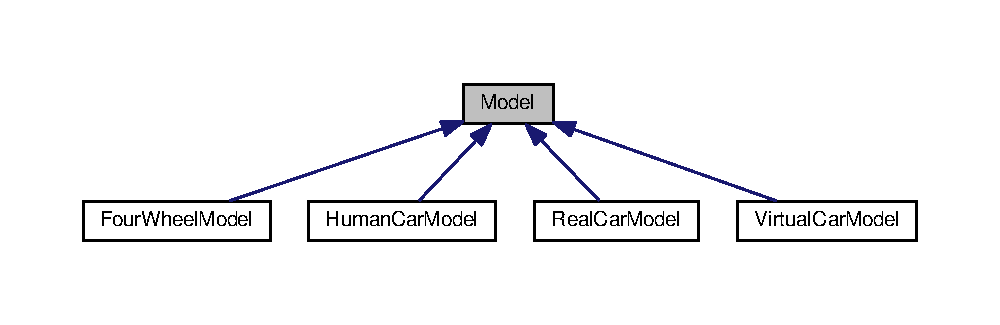
\includegraphics[width=350pt]{classModel__inherit__graph}
\end{center}
\end{figure}
\subsection*{Public Member Functions}
\begin{DoxyCompactItemize}
\item 
\hyperlink{classModel_ad9b9c0a0880f02066bcc3e1e4fba4319}{Model} (int \hyperlink{classModel_a863cbb90f0192bfdaced9d15c6757890}{dim\+State}, int \hyperlink{classModel_a0fd04d08ff3bdafdaf747713ffc824f0}{dim\+Intermediate})
\item 
virtual \hyperlink{Agent_8hpp_a5dd127bb3cb18b011cf5fd80a906e830}{Vector} \hyperlink{classModel_a887e642d0c195b771af8300c7c817f09}{update} (\hyperlink{Agent_8hpp_a5dd127bb3cb18b011cf5fd80a906e830}{Vector} state, \hyperlink{Agent_8hpp_a5dd127bb3cb18b011cf5fd80a906e830}{Vector} intermediate)=0
\end{DoxyCompactItemize}
\subsection*{Protected Attributes}
\begin{DoxyCompactItemize}
\item 
const int \hyperlink{classModel_a863cbb90f0192bfdaced9d15c6757890}{dim\+State}
\item 
const int \hyperlink{classModel_a0fd04d08ff3bdafdaf747713ffc824f0}{dim\+Intermediate}
\end{DoxyCompactItemize}


\subsection{Detailed Description}
Parent class for all models. 

\subsection{Constructor \& Destructor Documentation}
\index{Model@{Model}!Model@{Model}}
\index{Model@{Model}!Model@{Model}}
\subsubsection[{\texorpdfstring{Model(int dim\+State, int dim\+Intermediate)}{Model(int dimState, int dimIntermediate)}}]{\setlength{\rightskip}{0pt plus 5cm}Model\+::\+Model (
\begin{DoxyParamCaption}
\item[{int}]{dim\+State, }
\item[{int}]{dim\+Intermediate}
\end{DoxyParamCaption}
)\hspace{0.3cm}{\ttfamily [explicit]}}\hypertarget{classModel_ad9b9c0a0880f02066bcc3e1e4fba4319}{}\label{classModel_ad9b9c0a0880f02066bcc3e1e4fba4319}
Constructor. 
\begin{DoxyParams}{Parameters}
{\em dim\+State} & dimension of the state vector. \\
\hline
{\em dim\+Intermediate} & dimension of the intermediate vector. \\
\hline
\end{DoxyParams}


\subsection{Member Function Documentation}
\index{Model@{Model}!update@{update}}
\index{update@{update}!Model@{Model}}
\subsubsection[{\texorpdfstring{update(\+Vector state, Vector intermediate)=0}{update(Vector state, Vector intermediate)=0}}]{\setlength{\rightskip}{0pt plus 5cm}virtual {\bf Vector} Model\+::update (
\begin{DoxyParamCaption}
\item[{{\bf Vector}}]{state, }
\item[{{\bf Vector}}]{intermediate}
\end{DoxyParamCaption}
)\hspace{0.3cm}{\ttfamily [pure virtual]}}\hypertarget{classModel_a887e642d0c195b771af8300c7c817f09}{}\label{classModel_a887e642d0c195b771af8300c7c817f09}


Implemented in \hyperlink{classFourWheelModel_a2169e82abcb344e4bb345c563e6ea7de}{Four\+Wheel\+Model}, \hyperlink{classRealCarModel_a4437d9515709862a19fdd5f7e828d757}{Real\+Car\+Model}, \hyperlink{classHumanCarModel_aeaa782fab7b9ea5d9b245df0ced2b7cb}{Human\+Car\+Model}, and \hyperlink{classVirtualCarModel_ab7a61fe2ce2180bd330dbf2819249457}{Virtual\+Car\+Model}.



\subsection{Member Data Documentation}
\index{Model@{Model}!dim\+Intermediate@{dim\+Intermediate}}
\index{dim\+Intermediate@{dim\+Intermediate}!Model@{Model}}
\subsubsection[{\texorpdfstring{dim\+Intermediate}{dimIntermediate}}]{\setlength{\rightskip}{0pt plus 5cm}const int Model\+::dim\+Intermediate\hspace{0.3cm}{\ttfamily [protected]}}\hypertarget{classModel_a0fd04d08ff3bdafdaf747713ffc824f0}{}\label{classModel_a0fd04d08ff3bdafdaf747713ffc824f0}
dimension of the intermediate vector. \index{Model@{Model}!dim\+State@{dim\+State}}
\index{dim\+State@{dim\+State}!Model@{Model}}
\subsubsection[{\texorpdfstring{dim\+State}{dimState}}]{\setlength{\rightskip}{0pt plus 5cm}const int Model\+::dim\+State\hspace{0.3cm}{\ttfamily [protected]}}\hypertarget{classModel_a863cbb90f0192bfdaced9d15c6757890}{}\label{classModel_a863cbb90f0192bfdaced9d15c6757890}
dimension of the state vector. 

The documentation for this class was generated from the following files\+:\begin{DoxyCompactItemize}
\item 
Models/\hyperlink{Model_8hpp}{Model.\+hpp}\item 
Models/\hyperlink{Model_8cpp}{Model.\+cpp}\end{DoxyCompactItemize}

\hypertarget{classMyThread}{}\section{My\+Thread Class Reference}
\label{classMyThread}\index{My\+Thread@{My\+Thread}}


The class of Mythread.  




{\ttfamily \#include $<$My\+Thread.\+hpp$>$}



Collaboration diagram for My\+Thread\+:\nopagebreak
\begin{figure}[H]
\begin{center}
\leavevmode
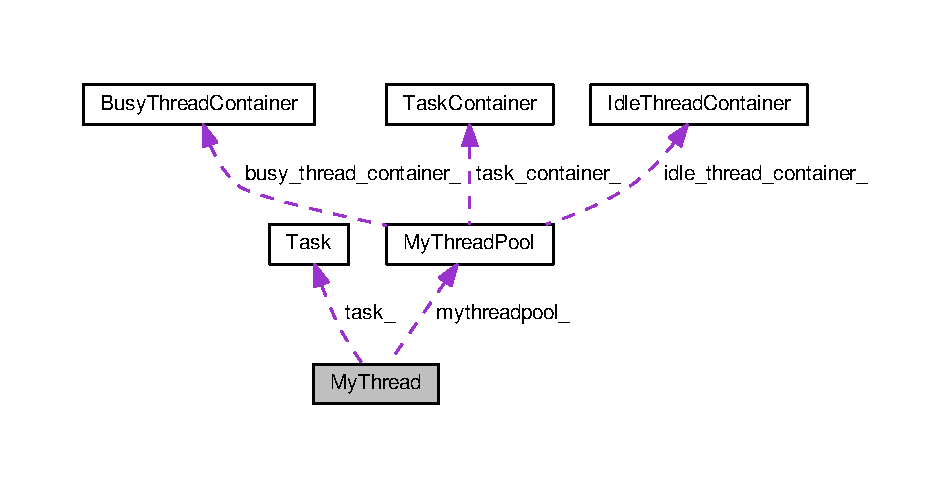
\includegraphics[width=350pt]{classMyThread__coll__graph}
\end{center}
\end{figure}
\subsection*{Public Member Functions}
\begin{DoxyCompactItemize}
\item 
\hyperlink{classMyThread_a43018638650ded91b9a511132a96f778}{My\+Thread} (\hyperlink{classMyThreadPool}{My\+Thread\+Pool} $\ast$pool)
\item 
void \hyperlink{classMyThread_adadb69384a54610a8c7affebcfbb0133}{Assign} (\hyperlink{classTask}{Task} $\ast$\hyperlink{classTask}{Task})
\begin{DoxyCompactList}\small\item\em Assign a task to the thread. \end{DoxyCompactList}\item 
void \hyperlink{classMyThread_a3f9f6783bbe4de36b1248cc5a493366a}{Run} ()
\begin{DoxyCompactList}\small\item\em Run method of thread. \end{DoxyCompactList}\item 
void \hyperlink{classMyThread_a939eae525c8a51ccb2116b940197185a}{Start\+Thread} ()
\begin{DoxyCompactList}\small\item\em Start a thread. \end{DoxyCompactList}\item 
int \hyperlink{classMyThread_a147606088b0b0479f706bf23dbb77a50}{getthreadid} ()
\begin{DoxyCompactList}\small\item\em Get id of a thread. \end{DoxyCompactList}\item 
void \hyperlink{classMyThread_a619a32097b4bd211d7238f15f3e5f2c3}{setisdetach} (bool isdetach)
\begin{DoxyCompactList}\small\item\em Set thread to detach. \end{DoxyCompactList}\end{DoxyCompactItemize}
\subsection*{Private Attributes}
\begin{DoxyCompactItemize}
\item 
\hyperlink{classMyThreadPool}{My\+Thread\+Pool} $\ast$ \hyperlink{classMyThread_a74d5590119c9211bd47b2ec9adaafc02}{mythreadpool\+\_\+}
\item 
bool \hyperlink{classMyThread_ad64c87d4924eab30ae36bed5d3560dfc}{isdetach\+\_\+}
\item 
\hyperlink{classTask}{Task} $\ast$ \hyperlink{classMyThread_a1013bd0ea254f26c337d8e35dd1c5762}{task\+\_\+}
\item 
int \hyperlink{classMyThread_a4ab4d45dabcb1c302ad03b9b8dbda282}{threadid\+\_\+}
\item 
std\+::thread \hyperlink{classMyThread_afb1913aba4cad629b8c6e1de298abfea}{thread\+\_\+}
\end{DoxyCompactItemize}
\subsection*{Static Private Attributes}
\begin{DoxyCompactItemize}
\item 
static int \hyperlink{classMyThread_acbc8ee4da3256965f79235c1c4723623}{s\+\_\+threadnumber} = 0
\end{DoxyCompactItemize}
\subsection*{Friends}
\begin{DoxyCompactItemize}
\item 
bool \hyperlink{classMyThread_a15f0b275ae59d106b8b71ecde1c8bf85}{operator==} (\hyperlink{classMyThread}{My\+Thread} my1, \hyperlink{classMyThread}{My\+Thread} my2)
\item 
bool \hyperlink{classMyThread_a32824be738942485e360599a05f15782}{operator!=} (\hyperlink{classMyThread}{My\+Thread} my1, \hyperlink{classMyThread}{My\+Thread} my2)
\end{DoxyCompactItemize}


\subsection{Detailed Description}
The class of Mythread. 

It manage one thread 

\subsection{Constructor \& Destructor Documentation}
\index{My\+Thread@{My\+Thread}!My\+Thread@{My\+Thread}}
\index{My\+Thread@{My\+Thread}!My\+Thread@{My\+Thread}}
\subsubsection[{\texorpdfstring{My\+Thread(\+My\+Thread\+Pool $\ast$pool)}{MyThread(MyThreadPool *pool)}}]{\setlength{\rightskip}{0pt plus 5cm}My\+Thread\+::\+My\+Thread (
\begin{DoxyParamCaption}
\item[{{\bf My\+Thread\+Pool} $\ast$}]{pool}
\end{DoxyParamCaption}
)}\hypertarget{classMyThread_a43018638650ded91b9a511132a96f778}{}\label{classMyThread_a43018638650ded91b9a511132a96f778}

\begin{DoxyParams}{Parameters}
{\em pool} & reference to the threadpool. \\
\hline
\end{DoxyParams}


\subsection{Member Function Documentation}
\index{My\+Thread@{My\+Thread}!Assign@{Assign}}
\index{Assign@{Assign}!My\+Thread@{My\+Thread}}
\subsubsection[{\texorpdfstring{Assign(\+Task $\ast$\+Task)}{Assign(Task *Task)}}]{\setlength{\rightskip}{0pt plus 5cm}void My\+Thread\+::\+Assign (
\begin{DoxyParamCaption}
\item[{{\bf Task} $\ast$}]{Task}
\end{DoxyParamCaption}
)}\hypertarget{classMyThread_adadb69384a54610a8c7affebcfbb0133}{}\label{classMyThread_adadb69384a54610a8c7affebcfbb0133}


Assign a task to the thread. 

\index{My\+Thread@{My\+Thread}!getthreadid@{getthreadid}}
\index{getthreadid@{getthreadid}!My\+Thread@{My\+Thread}}
\subsubsection[{\texorpdfstring{getthreadid()}{getthreadid()}}]{\setlength{\rightskip}{0pt plus 5cm}int My\+Thread\+::getthreadid (
\begin{DoxyParamCaption}
{}
\end{DoxyParamCaption}
)}\hypertarget{classMyThread_a147606088b0b0479f706bf23dbb77a50}{}\label{classMyThread_a147606088b0b0479f706bf23dbb77a50}


Get id of a thread. 

\index{My\+Thread@{My\+Thread}!Run@{Run}}
\index{Run@{Run}!My\+Thread@{My\+Thread}}
\subsubsection[{\texorpdfstring{Run()}{Run()}}]{\setlength{\rightskip}{0pt plus 5cm}void My\+Thread\+::\+Run (
\begin{DoxyParamCaption}
{}
\end{DoxyParamCaption}
)}\hypertarget{classMyThread_a3f9f6783bbe4de36b1248cc5a493366a}{}\label{classMyThread_a3f9f6783bbe4de36b1248cc5a493366a}


Run method of thread. 

\index{My\+Thread@{My\+Thread}!setisdetach@{setisdetach}}
\index{setisdetach@{setisdetach}!My\+Thread@{My\+Thread}}
\subsubsection[{\texorpdfstring{setisdetach(bool isdetach)}{setisdetach(bool isdetach)}}]{\setlength{\rightskip}{0pt plus 5cm}void My\+Thread\+::setisdetach (
\begin{DoxyParamCaption}
\item[{bool}]{isdetach}
\end{DoxyParamCaption}
)}\hypertarget{classMyThread_a619a32097b4bd211d7238f15f3e5f2c3}{}\label{classMyThread_a619a32097b4bd211d7238f15f3e5f2c3}


Set thread to detach. 

\index{My\+Thread@{My\+Thread}!Start\+Thread@{Start\+Thread}}
\index{Start\+Thread@{Start\+Thread}!My\+Thread@{My\+Thread}}
\subsubsection[{\texorpdfstring{Start\+Thread()}{StartThread()}}]{\setlength{\rightskip}{0pt plus 5cm}void My\+Thread\+::\+Start\+Thread (
\begin{DoxyParamCaption}
{}
\end{DoxyParamCaption}
)}\hypertarget{classMyThread_a939eae525c8a51ccb2116b940197185a}{}\label{classMyThread_a939eae525c8a51ccb2116b940197185a}


Start a thread. 



\subsection{Friends And Related Function Documentation}
\index{My\+Thread@{My\+Thread}!operator"!=@{operator"!=}}
\index{operator"!=@{operator"!=}!My\+Thread@{My\+Thread}}
\subsubsection[{\texorpdfstring{operator"!=}{operator!=}}]{\setlength{\rightskip}{0pt plus 5cm}bool operator!= (
\begin{DoxyParamCaption}
\item[{{\bf My\+Thread}}]{my1, }
\item[{{\bf My\+Thread}}]{my2}
\end{DoxyParamCaption}
)\hspace{0.3cm}{\ttfamily [friend]}}\hypertarget{classMyThread_a32824be738942485e360599a05f15782}{}\label{classMyThread_a32824be738942485e360599a05f15782}
\index{My\+Thread@{My\+Thread}!operator==@{operator==}}
\index{operator==@{operator==}!My\+Thread@{My\+Thread}}
\subsubsection[{\texorpdfstring{operator==}{operator==}}]{\setlength{\rightskip}{0pt plus 5cm}bool operator== (
\begin{DoxyParamCaption}
\item[{{\bf My\+Thread}}]{my1, }
\item[{{\bf My\+Thread}}]{my2}
\end{DoxyParamCaption}
)\hspace{0.3cm}{\ttfamily [friend]}}\hypertarget{classMyThread_a15f0b275ae59d106b8b71ecde1c8bf85}{}\label{classMyThread_a15f0b275ae59d106b8b71ecde1c8bf85}


\subsection{Member Data Documentation}
\index{My\+Thread@{My\+Thread}!isdetach\+\_\+@{isdetach\+\_\+}}
\index{isdetach\+\_\+@{isdetach\+\_\+}!My\+Thread@{My\+Thread}}
\subsubsection[{\texorpdfstring{isdetach\+\_\+}{isdetach_}}]{\setlength{\rightskip}{0pt plus 5cm}bool My\+Thread\+::isdetach\+\_\+\hspace{0.3cm}{\ttfamily [private]}}\hypertarget{classMyThread_ad64c87d4924eab30ae36bed5d3560dfc}{}\label{classMyThread_ad64c87d4924eab30ae36bed5d3560dfc}
Flag for thread whether detach or join. \index{My\+Thread@{My\+Thread}!mythreadpool\+\_\+@{mythreadpool\+\_\+}}
\index{mythreadpool\+\_\+@{mythreadpool\+\_\+}!My\+Thread@{My\+Thread}}
\subsubsection[{\texorpdfstring{mythreadpool\+\_\+}{mythreadpool_}}]{\setlength{\rightskip}{0pt plus 5cm}{\bf My\+Thread\+Pool}$\ast$ My\+Thread\+::mythreadpool\+\_\+\hspace{0.3cm}{\ttfamily [private]}}\hypertarget{classMyThread_a74d5590119c9211bd47b2ec9adaafc02}{}\label{classMyThread_a74d5590119c9211bd47b2ec9adaafc02}
The thread pool this thread signed in. \index{My\+Thread@{My\+Thread}!s\+\_\+threadnumber@{s\+\_\+threadnumber}}
\index{s\+\_\+threadnumber@{s\+\_\+threadnumber}!My\+Thread@{My\+Thread}}
\subsubsection[{\texorpdfstring{s\+\_\+threadnumber}{s_threadnumber}}]{\setlength{\rightskip}{0pt plus 5cm}int My\+Thread\+::s\+\_\+threadnumber = 0\hspace{0.3cm}{\ttfamily [static]}, {\ttfamily [private]}}\hypertarget{classMyThread_acbc8ee4da3256965f79235c1c4723623}{}\label{classMyThread_acbc8ee4da3256965f79235c1c4723623}
An counter for Mythraed to get different id for thread ID \index{My\+Thread@{My\+Thread}!task\+\_\+@{task\+\_\+}}
\index{task\+\_\+@{task\+\_\+}!My\+Thread@{My\+Thread}}
\subsubsection[{\texorpdfstring{task\+\_\+}{task_}}]{\setlength{\rightskip}{0pt plus 5cm}{\bf Task}$\ast$ My\+Thread\+::task\+\_\+\hspace{0.3cm}{\ttfamily [private]}}\hypertarget{classMyThread_a1013bd0ea254f26c337d8e35dd1c5762}{}\label{classMyThread_a1013bd0ea254f26c337d8e35dd1c5762}
The task that the thread will handle. \index{My\+Thread@{My\+Thread}!thread\+\_\+@{thread\+\_\+}}
\index{thread\+\_\+@{thread\+\_\+}!My\+Thread@{My\+Thread}}
\subsubsection[{\texorpdfstring{thread\+\_\+}{thread_}}]{\setlength{\rightskip}{0pt plus 5cm}std\+::thread My\+Thread\+::thread\+\_\+\hspace{0.3cm}{\ttfamily [private]}}\hypertarget{classMyThread_afb1913aba4cad629b8c6e1de298abfea}{}\label{classMyThread_afb1913aba4cad629b8c6e1de298abfea}
Thread itself \index{My\+Thread@{My\+Thread}!threadid\+\_\+@{threadid\+\_\+}}
\index{threadid\+\_\+@{threadid\+\_\+}!My\+Thread@{My\+Thread}}
\subsubsection[{\texorpdfstring{threadid\+\_\+}{threadid_}}]{\setlength{\rightskip}{0pt plus 5cm}int My\+Thread\+::threadid\+\_\+\hspace{0.3cm}{\ttfamily [private]}}\hypertarget{classMyThread_a4ab4d45dabcb1c302ad03b9b8dbda282}{}\label{classMyThread_a4ab4d45dabcb1c302ad03b9b8dbda282}
Thread ID 

The documentation for this class was generated from the following files\+:\begin{DoxyCompactItemize}
\item 
thread\+Pool/\hyperlink{MyThread_8hpp}{My\+Thread.\+hpp}\item 
thread\+Pool/\hyperlink{MyThread_8cpp}{My\+Thread.\+cpp}\end{DoxyCompactItemize}

\hypertarget{classMyThreadPool}{}\section{My\+Thread\+Pool Class Reference}
\label{classMyThreadPool}\index{My\+Thread\+Pool@{My\+Thread\+Pool}}


The class of the thread pool.  




{\ttfamily \#include $<$My\+Thread\+Pool.\+hpp$>$}



Collaboration diagram for My\+Thread\+Pool\+:\nopagebreak
\begin{figure}[H]
\begin{center}
\leavevmode
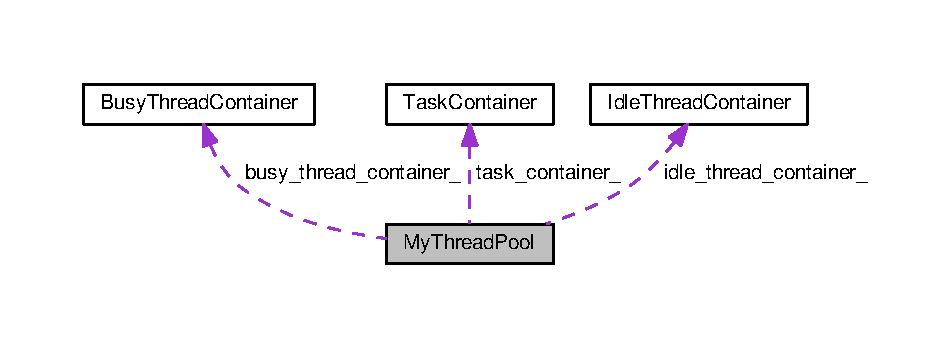
\includegraphics[width=350pt]{classMyThreadPool__coll__graph}
\end{center}
\end{figure}
\subsection*{Public Member Functions}
\begin{DoxyCompactItemize}
\item 
\hyperlink{classMyThreadPool_a04294a435753b308cf6824a75d74276c}{My\+Thread\+Pool} ()
\item 
\hyperlink{classMyThreadPool_a40cbc85efab055210ea6d877a22cc39a}{My\+Thread\+Pool} (int number)
\item 
\hyperlink{classMyThreadPool_aa5b063c10015672f734136a04aad676c}{$\sim$\+My\+Thread\+Pool} ()
\item 
void \hyperlink{classMyThreadPool_a374ac295e70a29caa3da47f58c2342ac}{Add\+Task} (\hyperlink{classTask}{Task} $\ast$\hyperlink{classTask}{Task}, int priority)
\begin{DoxyCompactList}\small\item\em Add a task to the thread pool. \end{DoxyCompactList}\item 
void \hyperlink{classMyThreadPool_aae8e3a40bf8be12e3dd5511f5d294b89}{Add\+Idle\+Thread} (int n)
\begin{DoxyCompactList}\small\item\em Add an idle thread to the thread pool. \end{DoxyCompactList}\item 
void \hyperlink{classMyThreadPool_afacd09493b96072c1201458b77f91ea9}{Remove\+Thread\+From\+Busy} (\hyperlink{classMyThread}{My\+Thread} $\ast$my\+Thread)
\begin{DoxyCompactList}\small\item\em Remove a thread from busy thread container. \end{DoxyCompactList}\item 
void \hyperlink{classMyThreadPool_a821cbd5122c8c1b13468d98a41497bdf}{Start} ()
\item 
void \hyperlink{classMyThreadPool_a9cda728b68b6a0f6c7447b7278e589ff}{End\+My\+Thread\+Pool} ()
\begin{DoxyCompactList}\small\item\em End the thread pool. \end{DoxyCompactList}\end{DoxyCompactItemize}
\subsection*{Private Attributes}
\begin{DoxyCompactItemize}
\item 
\hyperlink{classBusyThreadContainer}{Busy\+Thread\+Container} \hyperlink{classMyThreadPool_a13599d8e76159af56c216e04c69aa4a5}{busy\+\_\+thread\+\_\+container\+\_\+}
\item 
\hyperlink{classIdleThreadContainer}{Idle\+Thread\+Container} \hyperlink{classMyThreadPool_a9bcb3aebe659a0e30d9ab80ace409716}{idle\+\_\+thread\+\_\+container\+\_\+}
\item 
bool \hyperlink{classMyThreadPool_acd750861efa8ae618fc9c88bea24382d}{issurvive\+\_\+}
\item 
\hyperlink{classTaskContainer}{Task\+Container} \hyperlink{classMyThreadPool_a2dcc9c71c8674944854b7b9a494e0efe}{task\+\_\+container\+\_\+}
\item 
std\+::thread \hyperlink{classMyThreadPool_a3ce4bece158ca272e1acf88a9f25cde4}{thread\+\_\+this\+\_\+}
\item 
std\+::mutex \hyperlink{classMyThreadPool_a2da6197d60ec1bef94218697eb42c264}{busy\+\_\+mutex\+\_\+}
\item 
std\+::mutex \hyperlink{classMyThreadPool_a9fa6f068a873d87b9967db1ae79f9e36}{idle\+\_\+mutex\+\_\+}
\item 
std\+::mutex \hyperlink{classMyThreadPool_abf915ad66f55fbfb61d5b9693cc2f6d6}{task\+\_\+mutex\+\_\+}
\item 
int \hyperlink{classMyThreadPool_ad290954c3ceb2c991732961b895098ec}{number\+\_\+of\+\_\+thread\+\_\+}
\end{DoxyCompactItemize}


\subsection{Detailed Description}
The class of the thread pool. 

It manages all thread for calculating agents. 

\subsection{Constructor \& Destructor Documentation}
\index{My\+Thread\+Pool@{My\+Thread\+Pool}!My\+Thread\+Pool@{My\+Thread\+Pool}}
\index{My\+Thread\+Pool@{My\+Thread\+Pool}!My\+Thread\+Pool@{My\+Thread\+Pool}}
\subsubsection[{\texorpdfstring{My\+Thread\+Pool()}{MyThreadPool()}}]{\setlength{\rightskip}{0pt plus 5cm}My\+Thread\+Pool\+::\+My\+Thread\+Pool (
\begin{DoxyParamCaption}
{}
\end{DoxyParamCaption}
)\hspace{0.3cm}{\ttfamily [inline]}}\hypertarget{classMyThreadPool_a04294a435753b308cf6824a75d74276c}{}\label{classMyThreadPool_a04294a435753b308cf6824a75d74276c}
\index{My\+Thread\+Pool@{My\+Thread\+Pool}!My\+Thread\+Pool@{My\+Thread\+Pool}}
\index{My\+Thread\+Pool@{My\+Thread\+Pool}!My\+Thread\+Pool@{My\+Thread\+Pool}}
\subsubsection[{\texorpdfstring{My\+Thread\+Pool(int number)}{MyThreadPool(int number)}}]{\setlength{\rightskip}{0pt plus 5cm}My\+Thread\+Pool\+::\+My\+Thread\+Pool (
\begin{DoxyParamCaption}
\item[{int}]{number}
\end{DoxyParamCaption}
)}\hypertarget{classMyThreadPool_a40cbc85efab055210ea6d877a22cc39a}{}\label{classMyThreadPool_a40cbc85efab055210ea6d877a22cc39a}

\begin{DoxyParams}{Parameters}
{\em number} & reference to the number of threads in the thread pool. \\
\hline
\end{DoxyParams}
\index{My\+Thread\+Pool@{My\+Thread\+Pool}!````~My\+Thread\+Pool@{$\sim$\+My\+Thread\+Pool}}
\index{````~My\+Thread\+Pool@{$\sim$\+My\+Thread\+Pool}!My\+Thread\+Pool@{My\+Thread\+Pool}}
\subsubsection[{\texorpdfstring{$\sim$\+My\+Thread\+Pool()}{~MyThreadPool()}}]{\setlength{\rightskip}{0pt plus 5cm}My\+Thread\+Pool\+::$\sim$\+My\+Thread\+Pool (
\begin{DoxyParamCaption}
{}
\end{DoxyParamCaption}
)}\hypertarget{classMyThreadPool_aa5b063c10015672f734136a04aad676c}{}\label{classMyThreadPool_aa5b063c10015672f734136a04aad676c}


\subsection{Member Function Documentation}
\index{My\+Thread\+Pool@{My\+Thread\+Pool}!Add\+Idle\+Thread@{Add\+Idle\+Thread}}
\index{Add\+Idle\+Thread@{Add\+Idle\+Thread}!My\+Thread\+Pool@{My\+Thread\+Pool}}
\subsubsection[{\texorpdfstring{Add\+Idle\+Thread(int n)}{AddIdleThread(int n)}}]{\setlength{\rightskip}{0pt plus 5cm}void My\+Thread\+Pool\+::\+Add\+Idle\+Thread (
\begin{DoxyParamCaption}
\item[{int}]{n}
\end{DoxyParamCaption}
)}\hypertarget{classMyThreadPool_aae8e3a40bf8be12e3dd5511f5d294b89}{}\label{classMyThreadPool_aae8e3a40bf8be12e3dd5511f5d294b89}


Add an idle thread to the thread pool. 

\index{My\+Thread\+Pool@{My\+Thread\+Pool}!Add\+Task@{Add\+Task}}
\index{Add\+Task@{Add\+Task}!My\+Thread\+Pool@{My\+Thread\+Pool}}
\subsubsection[{\texorpdfstring{Add\+Task(\+Task $\ast$\+Task, int priority)}{AddTask(Task *Task, int priority)}}]{\setlength{\rightskip}{0pt plus 5cm}void My\+Thread\+Pool\+::\+Add\+Task (
\begin{DoxyParamCaption}
\item[{{\bf Task} $\ast$}]{Task, }
\item[{int}]{priority = {\ttfamily (PRIORITY\+:\+:NORMAL)}}
\end{DoxyParamCaption}
)}\hypertarget{classMyThreadPool_a374ac295e70a29caa3da47f58c2342ac}{}\label{classMyThreadPool_a374ac295e70a29caa3da47f58c2342ac}


Add a task to the thread pool. 

\index{My\+Thread\+Pool@{My\+Thread\+Pool}!End\+My\+Thread\+Pool@{End\+My\+Thread\+Pool}}
\index{End\+My\+Thread\+Pool@{End\+My\+Thread\+Pool}!My\+Thread\+Pool@{My\+Thread\+Pool}}
\subsubsection[{\texorpdfstring{End\+My\+Thread\+Pool()}{EndMyThreadPool()}}]{\setlength{\rightskip}{0pt plus 5cm}void My\+Thread\+Pool\+::\+End\+My\+Thread\+Pool (
\begin{DoxyParamCaption}
{}
\end{DoxyParamCaption}
)}\hypertarget{classMyThreadPool_a9cda728b68b6a0f6c7447b7278e589ff}{}\label{classMyThreadPool_a9cda728b68b6a0f6c7447b7278e589ff}


End the thread pool. 

\index{My\+Thread\+Pool@{My\+Thread\+Pool}!Remove\+Thread\+From\+Busy@{Remove\+Thread\+From\+Busy}}
\index{Remove\+Thread\+From\+Busy@{Remove\+Thread\+From\+Busy}!My\+Thread\+Pool@{My\+Thread\+Pool}}
\subsubsection[{\texorpdfstring{Remove\+Thread\+From\+Busy(\+My\+Thread $\ast$my\+Thread)}{RemoveThreadFromBusy(MyThread *myThread)}}]{\setlength{\rightskip}{0pt plus 5cm}void My\+Thread\+Pool\+::\+Remove\+Thread\+From\+Busy (
\begin{DoxyParamCaption}
\item[{{\bf My\+Thread} $\ast$}]{my\+Thread}
\end{DoxyParamCaption}
)}\hypertarget{classMyThreadPool_afacd09493b96072c1201458b77f91ea9}{}\label{classMyThreadPool_afacd09493b96072c1201458b77f91ea9}


Remove a thread from busy thread container. 

\index{My\+Thread\+Pool@{My\+Thread\+Pool}!Start@{Start}}
\index{Start@{Start}!My\+Thread\+Pool@{My\+Thread\+Pool}}
\subsubsection[{\texorpdfstring{Start()}{Start()}}]{\setlength{\rightskip}{0pt plus 5cm}void My\+Thread\+Pool\+::\+Start (
\begin{DoxyParamCaption}
{}
\end{DoxyParamCaption}
)}\hypertarget{classMyThreadPool_a821cbd5122c8c1b13468d98a41497bdf}{}\label{classMyThreadPool_a821cbd5122c8c1b13468d98a41497bdf}
Start the thread pool. It will keep scan whether exists idle threads in idle\+\_\+thread\+\_\+container\+\_\+ and invoke idle threads to handle tasks and put that thread into busy\+\_\+thread\+\_\+container\+\_\+. 

\subsection{Member Data Documentation}
\index{My\+Thread\+Pool@{My\+Thread\+Pool}!busy\+\_\+mutex\+\_\+@{busy\+\_\+mutex\+\_\+}}
\index{busy\+\_\+mutex\+\_\+@{busy\+\_\+mutex\+\_\+}!My\+Thread\+Pool@{My\+Thread\+Pool}}
\subsubsection[{\texorpdfstring{busy\+\_\+mutex\+\_\+}{busy_mutex_}}]{\setlength{\rightskip}{0pt plus 5cm}std\+::mutex My\+Thread\+Pool\+::busy\+\_\+mutex\+\_\+\hspace{0.3cm}{\ttfamily [private]}}\hypertarget{classMyThreadPool_a2da6197d60ec1bef94218697eb42c264}{}\label{classMyThreadPool_a2da6197d60ec1bef94218697eb42c264}
Mutex for busy\+\_\+thread\+\_\+container\+\_\+. \index{My\+Thread\+Pool@{My\+Thread\+Pool}!busy\+\_\+thread\+\_\+container\+\_\+@{busy\+\_\+thread\+\_\+container\+\_\+}}
\index{busy\+\_\+thread\+\_\+container\+\_\+@{busy\+\_\+thread\+\_\+container\+\_\+}!My\+Thread\+Pool@{My\+Thread\+Pool}}
\subsubsection[{\texorpdfstring{busy\+\_\+thread\+\_\+container\+\_\+}{busy_thread_container_}}]{\setlength{\rightskip}{0pt plus 5cm}{\bf Busy\+Thread\+Container} My\+Thread\+Pool\+::busy\+\_\+thread\+\_\+container\+\_\+\hspace{0.3cm}{\ttfamily [private]}}\hypertarget{classMyThreadPool_a13599d8e76159af56c216e04c69aa4a5}{}\label{classMyThreadPool_a13599d8e76159af56c216e04c69aa4a5}
Container for threads which is not in using. \index{My\+Thread\+Pool@{My\+Thread\+Pool}!idle\+\_\+mutex\+\_\+@{idle\+\_\+mutex\+\_\+}}
\index{idle\+\_\+mutex\+\_\+@{idle\+\_\+mutex\+\_\+}!My\+Thread\+Pool@{My\+Thread\+Pool}}
\subsubsection[{\texorpdfstring{idle\+\_\+mutex\+\_\+}{idle_mutex_}}]{\setlength{\rightskip}{0pt plus 5cm}std\+::mutex My\+Thread\+Pool\+::idle\+\_\+mutex\+\_\+\hspace{0.3cm}{\ttfamily [private]}}\hypertarget{classMyThreadPool_a9fa6f068a873d87b9967db1ae79f9e36}{}\label{classMyThreadPool_a9fa6f068a873d87b9967db1ae79f9e36}
Mutex for idle\+\_\+thread\+\_\+container\+\_\+. \index{My\+Thread\+Pool@{My\+Thread\+Pool}!idle\+\_\+thread\+\_\+container\+\_\+@{idle\+\_\+thread\+\_\+container\+\_\+}}
\index{idle\+\_\+thread\+\_\+container\+\_\+@{idle\+\_\+thread\+\_\+container\+\_\+}!My\+Thread\+Pool@{My\+Thread\+Pool}}
\subsubsection[{\texorpdfstring{idle\+\_\+thread\+\_\+container\+\_\+}{idle_thread_container_}}]{\setlength{\rightskip}{0pt plus 5cm}{\bf Idle\+Thread\+Container} My\+Thread\+Pool\+::idle\+\_\+thread\+\_\+container\+\_\+\hspace{0.3cm}{\ttfamily [private]}}\hypertarget{classMyThreadPool_a9bcb3aebe659a0e30d9ab80ace409716}{}\label{classMyThreadPool_a9bcb3aebe659a0e30d9ab80ace409716}
Container for threads which is in using. \index{My\+Thread\+Pool@{My\+Thread\+Pool}!issurvive\+\_\+@{issurvive\+\_\+}}
\index{issurvive\+\_\+@{issurvive\+\_\+}!My\+Thread\+Pool@{My\+Thread\+Pool}}
\subsubsection[{\texorpdfstring{issurvive\+\_\+}{issurvive_}}]{\setlength{\rightskip}{0pt plus 5cm}bool My\+Thread\+Pool\+::issurvive\+\_\+\hspace{0.3cm}{\ttfamily [private]}}\hypertarget{classMyThreadPool_acd750861efa8ae618fc9c88bea24382d}{}\label{classMyThreadPool_acd750861efa8ae618fc9c88bea24382d}
Flag for whether the thread pool is in using. \index{My\+Thread\+Pool@{My\+Thread\+Pool}!number\+\_\+of\+\_\+thread\+\_\+@{number\+\_\+of\+\_\+thread\+\_\+}}
\index{number\+\_\+of\+\_\+thread\+\_\+@{number\+\_\+of\+\_\+thread\+\_\+}!My\+Thread\+Pool@{My\+Thread\+Pool}}
\subsubsection[{\texorpdfstring{number\+\_\+of\+\_\+thread\+\_\+}{number_of_thread_}}]{\setlength{\rightskip}{0pt plus 5cm}int My\+Thread\+Pool\+::number\+\_\+of\+\_\+thread\+\_\+\hspace{0.3cm}{\ttfamily [private]}}\hypertarget{classMyThreadPool_ad290954c3ceb2c991732961b895098ec}{}\label{classMyThreadPool_ad290954c3ceb2c991732961b895098ec}
Number of threads in idle\+\_\+thread\+\_\+container\+\_\+ which means the maximum threads the thread pool can use simultaneously. \index{My\+Thread\+Pool@{My\+Thread\+Pool}!task\+\_\+container\+\_\+@{task\+\_\+container\+\_\+}}
\index{task\+\_\+container\+\_\+@{task\+\_\+container\+\_\+}!My\+Thread\+Pool@{My\+Thread\+Pool}}
\subsubsection[{\texorpdfstring{task\+\_\+container\+\_\+}{task_container_}}]{\setlength{\rightskip}{0pt plus 5cm}{\bf Task\+Container} My\+Thread\+Pool\+::task\+\_\+container\+\_\+\hspace{0.3cm}{\ttfamily [private]}}\hypertarget{classMyThreadPool_a2dcc9c71c8674944854b7b9a494e0efe}{}\label{classMyThreadPool_a2dcc9c71c8674944854b7b9a494e0efe}
Container for tasks. \index{My\+Thread\+Pool@{My\+Thread\+Pool}!task\+\_\+mutex\+\_\+@{task\+\_\+mutex\+\_\+}}
\index{task\+\_\+mutex\+\_\+@{task\+\_\+mutex\+\_\+}!My\+Thread\+Pool@{My\+Thread\+Pool}}
\subsubsection[{\texorpdfstring{task\+\_\+mutex\+\_\+}{task_mutex_}}]{\setlength{\rightskip}{0pt plus 5cm}std\+::mutex My\+Thread\+Pool\+::task\+\_\+mutex\+\_\+\hspace{0.3cm}{\ttfamily [private]}}\hypertarget{classMyThreadPool_abf915ad66f55fbfb61d5b9693cc2f6d6}{}\label{classMyThreadPool_abf915ad66f55fbfb61d5b9693cc2f6d6}
Mutex for task\+\_\+container\+\_\+. \index{My\+Thread\+Pool@{My\+Thread\+Pool}!thread\+\_\+this\+\_\+@{thread\+\_\+this\+\_\+}}
\index{thread\+\_\+this\+\_\+@{thread\+\_\+this\+\_\+}!My\+Thread\+Pool@{My\+Thread\+Pool}}
\subsubsection[{\texorpdfstring{thread\+\_\+this\+\_\+}{thread_this_}}]{\setlength{\rightskip}{0pt plus 5cm}std\+::thread My\+Thread\+Pool\+::thread\+\_\+this\+\_\+\hspace{0.3cm}{\ttfamily [private]}}\hypertarget{classMyThreadPool_a3ce4bece158ca272e1acf88a9f25cde4}{}\label{classMyThreadPool_a3ce4bece158ca272e1acf88a9f25cde4}
The thread for the thread pool manage all threads. 

The documentation for this class was generated from the following files\+:\begin{DoxyCompactItemize}
\item 
thread\+Pool/\hyperlink{MyThreadPool_8hpp}{My\+Thread\+Pool.\+hpp}\item 
thread\+Pool/\hyperlink{MyThreadPool_8cpp}{My\+Thread\+Pool.\+cpp}\end{DoxyCompactItemize}

\hypertarget{classPlanner}{}\section{Planner Class Reference}
\label{classPlanner}\index{Planner@{Planner}}


Parent class for all planners.  




{\ttfamily \#include $<$Planner.\+hpp$>$}



Inheritance diagram for Planner\+:\nopagebreak
\begin{figure}[H]
\begin{center}
\leavevmode
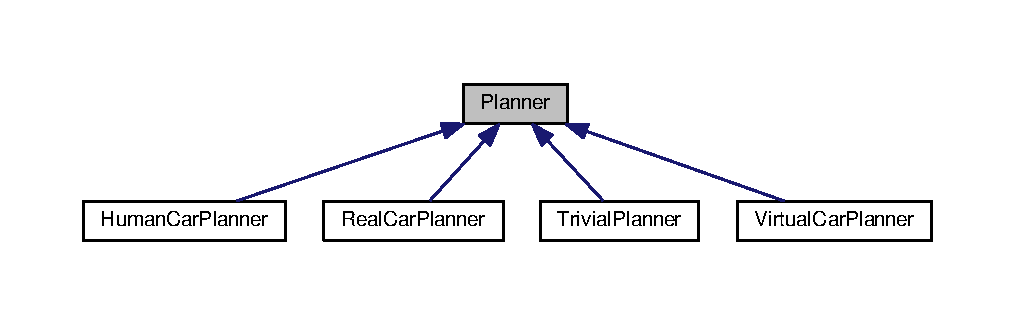
\includegraphics[width=350pt]{classPlanner__inherit__graph}
\end{center}
\end{figure}


Collaboration diagram for Planner\+:\nopagebreak
\begin{figure}[H]
\begin{center}
\leavevmode
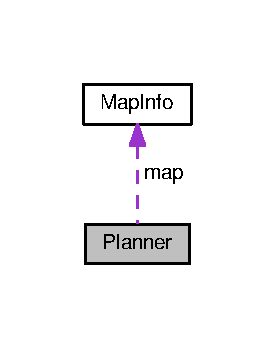
\includegraphics[width=132pt]{classPlanner__coll__graph}
\end{center}
\end{figure}
\subsection*{Public Member Functions}
\begin{DoxyCompactItemize}
\item 
\hyperlink{classPlanner_a010db2180841d3773eff05c3a760b029}{Planner} (int \hyperlink{classPlanner_a70081990e0749d5347190d37022c30f1}{dim\+State}, int \hyperlink{classPlanner_a4e6f8082d82e17c5821e26e12ab72421}{dim\+Input}, \hyperlink{classMapInfo}{Map\+Info} $\ast$\hyperlink{classPlanner_ab651f7a11072a2588bbb7683660b519e}{map}=nullptr)
\item 
virtual \hyperlink{Agent_8hpp_a5dd127bb3cb18b011cf5fd80a906e830}{Vector} \hyperlink{classPlanner_a62e1434402a3f36b0883e069a10447d8}{update} (\hyperlink{Agent_8hpp_a5dd127bb3cb18b011cf5fd80a906e830}{Vector} current\+State, const \hyperlink{Agent_8hpp_a5dd127bb3cb18b011cf5fd80a906e830}{Vector} \&human\+Input, std\+::vector$<$ \hyperlink{classAgent}{Agent} $\ast$ $>$ agents)=0
\end{DoxyCompactItemize}
\subsection*{Protected Attributes}
\begin{DoxyCompactItemize}
\item 
const int \hyperlink{classPlanner_a70081990e0749d5347190d37022c30f1}{dim\+State}
\item 
const int \hyperlink{classPlanner_a4e6f8082d82e17c5821e26e12ab72421}{dim\+Input}
\item 
const \hyperlink{classMapInfo}{Map\+Info} $\ast$ \hyperlink{classPlanner_ab651f7a11072a2588bbb7683660b519e}{map}
\end{DoxyCompactItemize}


\subsection{Detailed Description}
Parent class for all planners. 

\subsection{Constructor \& Destructor Documentation}
\index{Planner@{Planner}!Planner@{Planner}}
\index{Planner@{Planner}!Planner@{Planner}}
\subsubsection[{\texorpdfstring{Planner(int dim\+State, int dim\+Input, Map\+Info $\ast$map=nullptr)}{Planner(int dimState, int dimInput, MapInfo *map=nullptr)}}]{\setlength{\rightskip}{0pt plus 5cm}Planner\+::\+Planner (
\begin{DoxyParamCaption}
\item[{int}]{dim\+State, }
\item[{int}]{dim\+Input, }
\item[{{\bf Map\+Info} $\ast$}]{map = {\ttfamily nullptr}}
\end{DoxyParamCaption}
)\hspace{0.3cm}{\ttfamily [explicit]}}\hypertarget{classPlanner_a010db2180841d3773eff05c3a760b029}{}\label{classPlanner_a010db2180841d3773eff05c3a760b029}
Constructor. 
\begin{DoxyParams}{Parameters}
{\em dim\+State} & dimension of the state vector. \\
\hline
{\em dim\+Input} & dimension of the input vector. \\
\hline
\end{DoxyParams}


\subsection{Member Function Documentation}
\index{Planner@{Planner}!update@{update}}
\index{update@{update}!Planner@{Planner}}
\subsubsection[{\texorpdfstring{update(\+Vector current\+State, const Vector \&human\+Input, std\+::vector$<$ Agent $\ast$ $>$ agents)=0}{update(Vector currentState, const Vector &humanInput, std::vector< Agent * > agents)=0}}]{\setlength{\rightskip}{0pt plus 5cm}virtual {\bf Vector} Planner\+::update (
\begin{DoxyParamCaption}
\item[{{\bf Vector}}]{current\+State, }
\item[{const {\bf Vector} \&}]{human\+Input, }
\item[{std\+::vector$<$ {\bf Agent} $\ast$ $>$}]{agents}
\end{DoxyParamCaption}
)\hspace{0.3cm}{\ttfamily [pure virtual]}}\hypertarget{classPlanner_a62e1434402a3f36b0883e069a10447d8}{}\label{classPlanner_a62e1434402a3f36b0883e069a10447d8}


Implemented in \hyperlink{classRealCarPlanner_aa7c4658f35a2310fffbd6c49474c4714}{Real\+Car\+Planner}, \hyperlink{classHumanCarPlanner_ad6c513730ee6374f64d1cf5cdb842af1}{Human\+Car\+Planner}, \hyperlink{classTrivialPlanner_a27317c7986fd79906da5964dd893c5e9}{Trivial\+Planner}, and \hyperlink{classVirtualCarPlanner_aa8624e1c729ebe167ace773ed271b160}{Virtual\+Car\+Planner}.



\subsection{Member Data Documentation}
\index{Planner@{Planner}!dim\+Input@{dim\+Input}}
\index{dim\+Input@{dim\+Input}!Planner@{Planner}}
\subsubsection[{\texorpdfstring{dim\+Input}{dimInput}}]{\setlength{\rightskip}{0pt plus 5cm}const int Planner\+::dim\+Input\hspace{0.3cm}{\ttfamily [protected]}}\hypertarget{classPlanner_a4e6f8082d82e17c5821e26e12ab72421}{}\label{classPlanner_a4e6f8082d82e17c5821e26e12ab72421}
dimension of the input vector. \index{Planner@{Planner}!dim\+State@{dim\+State}}
\index{dim\+State@{dim\+State}!Planner@{Planner}}
\subsubsection[{\texorpdfstring{dim\+State}{dimState}}]{\setlength{\rightskip}{0pt plus 5cm}const int Planner\+::dim\+State\hspace{0.3cm}{\ttfamily [protected]}}\hypertarget{classPlanner_a70081990e0749d5347190d37022c30f1}{}\label{classPlanner_a70081990e0749d5347190d37022c30f1}
dimension of the state vector \index{Planner@{Planner}!map@{map}}
\index{map@{map}!Planner@{Planner}}
\subsubsection[{\texorpdfstring{map}{map}}]{\setlength{\rightskip}{0pt plus 5cm}const {\bf Map\+Info}$\ast$ Planner\+::map\hspace{0.3cm}{\ttfamily [protected]}}\hypertarget{classPlanner_ab651f7a11072a2588bbb7683660b519e}{}\label{classPlanner_ab651f7a11072a2588bbb7683660b519e}


The documentation for this class was generated from the following files\+:\begin{DoxyCompactItemize}
\item 
Planners/\hyperlink{Planner_8hpp}{Planner.\+hpp}\item 
Planners/\hyperlink{Planner_8cpp}{Planner.\+cpp}\end{DoxyCompactItemize}

\hypertarget{classRealCar}{}\section{Real\+Car Class Reference}
\label{classRealCar}\index{Real\+Car@{Real\+Car}}


{\ttfamily \#include $<$Real\+Car.\+hpp$>$}



Inheritance diagram for Real\+Car\+:\nopagebreak
\begin{figure}[H]
\begin{center}
\leavevmode
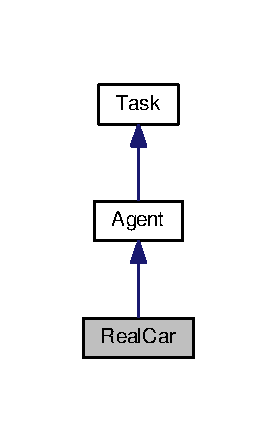
\includegraphics[width=133pt]{classRealCar__inherit__graph}
\end{center}
\end{figure}


Collaboration diagram for Real\+Car\+:\nopagebreak
\begin{figure}[H]
\begin{center}
\leavevmode
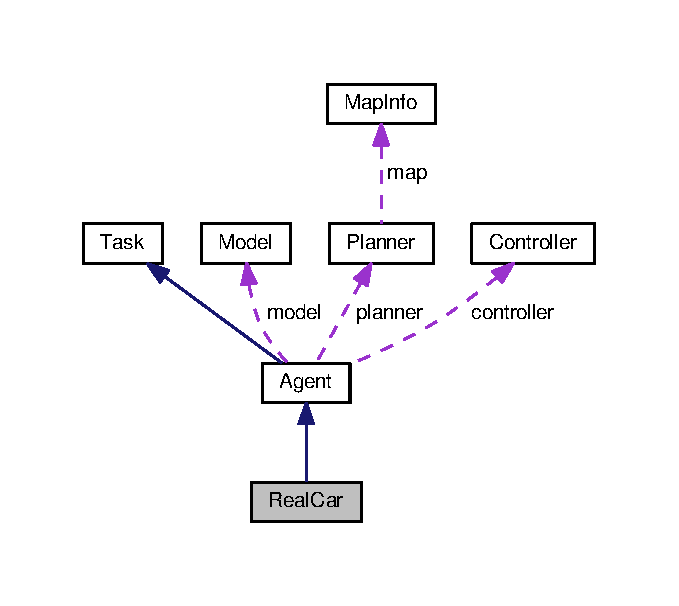
\includegraphics[width=326pt]{classRealCar__coll__graph}
\end{center}
\end{figure}
\subsection*{Public Member Functions}
\begin{DoxyCompactItemize}
\item 
\hyperlink{classRealCar_ac61f00960be11288d00dea7819df07b5}{Real\+Car} (int \hyperlink{classAgent_af8b58fe9dafe460ed2ddf87435a7feed}{id}, \hyperlink{Agent_8hpp_a5dd127bb3cb18b011cf5fd80a906e830}{Vector} initial\+State)
\item 
\hyperlink{classRealCar_a0663523335175d6369a69ef66449c7bd}{Real\+Car} (int \hyperlink{classAgent_af8b58fe9dafe460ed2ddf87435a7feed}{id}, \hyperlink{Agent_8hpp_a5dd127bb3cb18b011cf5fd80a906e830}{Vector} initial\+State, \hyperlink{classPlanner}{Planner} $\ast$\hyperlink{classAgent_aa71be9f465a3d8eed4e3297d8aa49eb1}{planner}, \hyperlink{classController}{Controller} $\ast$\hyperlink{classAgent_a35138f4fa7fa31760928b84680f7a886}{controller}, \hyperlink{classModel}{Model} $\ast$\hyperlink{classAgent_a41c7b65f7ad35cc6756cf0313edaa9a0}{model})
\item 
\hyperlink{Agent_8hpp_ad2c3439c0fbb853c45129639d2581c51}{Agent\+Type} \hyperlink{classRealCar_ab77ba7bc138ad5d1676a0562d44017f7}{get\+Type} () const override
\end{DoxyCompactItemize}
\subsection*{Additional Inherited Members}


\subsection{Detailed Description}
\hyperlink{classRealCar}{Real\+Car} is a kind of agent that is controlled by humans or autonomous driving program. It is the car in the testing ground. It moves in the real world and sends its states to this program. 

\subsection{Constructor \& Destructor Documentation}
\index{Real\+Car@{Real\+Car}!Real\+Car@{Real\+Car}}
\index{Real\+Car@{Real\+Car}!Real\+Car@{Real\+Car}}
\subsubsection[{\texorpdfstring{Real\+Car(int id, Vector initial\+State)}{RealCar(int id, Vector initialState)}}]{\setlength{\rightskip}{0pt plus 5cm}Real\+Car\+::\+Real\+Car (
\begin{DoxyParamCaption}
\item[{int}]{id, }
\item[{{\bf Vector}}]{initial\+State}
\end{DoxyParamCaption}
)}\hypertarget{classRealCar_ac61f00960be11288d00dea7819df07b5}{}\label{classRealCar_ac61f00960be11288d00dea7819df07b5}
\index{Real\+Car@{Real\+Car}!Real\+Car@{Real\+Car}}
\index{Real\+Car@{Real\+Car}!Real\+Car@{Real\+Car}}
\subsubsection[{\texorpdfstring{Real\+Car(int id, Vector initial\+State, Planner $\ast$planner, Controller $\ast$controller, Model $\ast$model)}{RealCar(int id, Vector initialState, Planner *planner, Controller *controller, Model *model)}}]{\setlength{\rightskip}{0pt plus 5cm}Real\+Car\+::\+Real\+Car (
\begin{DoxyParamCaption}
\item[{int}]{id, }
\item[{{\bf Vector}}]{initial\+State, }
\item[{{\bf Planner} $\ast$}]{planner, }
\item[{{\bf Controller} $\ast$}]{controller, }
\item[{{\bf Model} $\ast$}]{model}
\end{DoxyParamCaption}
)\hspace{0.3cm}{\ttfamily [explicit]}}\hypertarget{classRealCar_a0663523335175d6369a69ef66449c7bd}{}\label{classRealCar_a0663523335175d6369a69ef66449c7bd}
Constructor. 
\begin{DoxyParams}{Parameters}
{\em id} & id of the new real car. \\
\hline
{\em initial\+State} & initial state of the real car. \\
\hline
\end{DoxyParams}


\subsection{Member Function Documentation}
\index{Real\+Car@{Real\+Car}!get\+Type@{get\+Type}}
\index{get\+Type@{get\+Type}!Real\+Car@{Real\+Car}}
\subsubsection[{\texorpdfstring{get\+Type() const override}{getType() const override}}]{\setlength{\rightskip}{0pt plus 5cm}{\bf Agent\+Type} Real\+Car\+::get\+Type (
\begin{DoxyParamCaption}
{}
\end{DoxyParamCaption}
) const\hspace{0.3cm}{\ttfamily [override]}, {\ttfamily [virtual]}}\hypertarget{classRealCar_ab77ba7bc138ad5d1676a0562d44017f7}{}\label{classRealCar_ab77ba7bc138ad5d1676a0562d44017f7}
Type getter (overridden) \begin{DoxyReturn}{Returns}
type (real car) 
\end{DoxyReturn}


Implements \hyperlink{classAgent_a48eedea220997f4aa85ce4596f2c49c5}{Agent}.



The documentation for this class was generated from the following files\+:\begin{DoxyCompactItemize}
\item 
Agents/\hyperlink{RealCar_8hpp}{Real\+Car.\+hpp}\item 
Agents/\hyperlink{RealCar_8cpp}{Real\+Car.\+cpp}\end{DoxyCompactItemize}

\hypertarget{classRealCarController}{}\section{Real\+Car\+Controller Class Reference}
\label{classRealCarController}\index{Real\+Car\+Controller@{Real\+Car\+Controller}}


A \hyperlink{classRealCar}{Real\+Car} controller is the controller for the real car model (\hyperlink{classRealCarModel}{Real\+Car\+Model})  




{\ttfamily \#include $<$Real\+Car\+Controller.\+hpp$>$}



Inheritance diagram for Real\+Car\+Controller\+:\nopagebreak
\begin{figure}[H]
\begin{center}
\leavevmode
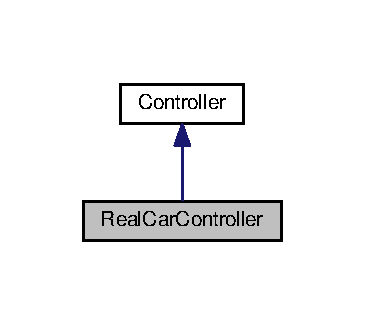
\includegraphics[width=175pt]{classRealCarController__inherit__graph}
\end{center}
\end{figure}


Collaboration diagram for Real\+Car\+Controller\+:\nopagebreak
\begin{figure}[H]
\begin{center}
\leavevmode
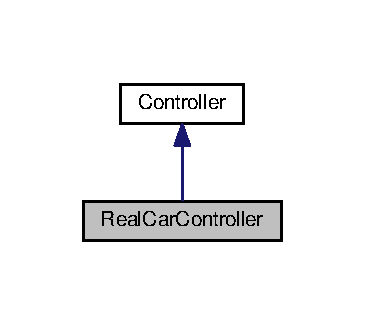
\includegraphics[width=175pt]{classRealCarController__coll__graph}
\end{center}
\end{figure}
\subsection*{Public Member Functions}
\begin{DoxyCompactItemize}
\item 
\hyperlink{classRealCarController_a475547f4307d78b33577d17a7b094363}{Real\+Car\+Controller} ()
\item 
\hyperlink{Agent_8hpp_a5dd127bb3cb18b011cf5fd80a906e830}{Vector} \hyperlink{classRealCarController_a639c0c911bbfc63ce90f9de2b8a9be4d}{update} (\hyperlink{Agent_8hpp_a5dd127bb3cb18b011cf5fd80a906e830}{Vector} input) override
\end{DoxyCompactItemize}
\subsection*{Additional Inherited Members}


\subsection{Detailed Description}
A \hyperlink{classRealCar}{Real\+Car} controller is the controller for the real car model (\hyperlink{classRealCarModel}{Real\+Car\+Model}) 

\subsection{Constructor \& Destructor Documentation}
\index{Real\+Car\+Controller@{Real\+Car\+Controller}!Real\+Car\+Controller@{Real\+Car\+Controller}}
\index{Real\+Car\+Controller@{Real\+Car\+Controller}!Real\+Car\+Controller@{Real\+Car\+Controller}}
\subsubsection[{\texorpdfstring{Real\+Car\+Controller()}{RealCarController()}}]{\setlength{\rightskip}{0pt plus 5cm}Real\+Car\+Controller\+::\+Real\+Car\+Controller (
\begin{DoxyParamCaption}
{}
\end{DoxyParamCaption}
)\hspace{0.3cm}{\ttfamily [explicit]}}\hypertarget{classRealCarController_a475547f4307d78b33577d17a7b094363}{}\label{classRealCarController_a475547f4307d78b33577d17a7b094363}
Constructor. Dimension of input vector is 3 (gas pedal, brake pedal, steering angle) Dimension of intermediate vector is 3. 

\subsection{Member Function Documentation}
\index{Real\+Car\+Controller@{Real\+Car\+Controller}!update@{update}}
\index{update@{update}!Real\+Car\+Controller@{Real\+Car\+Controller}}
\subsubsection[{\texorpdfstring{update(\+Vector input) override}{update(Vector input) override}}]{\setlength{\rightskip}{0pt plus 5cm}{\bf Vector} Real\+Car\+Controller\+::update (
\begin{DoxyParamCaption}
\item[{{\bf Vector}}]{input}
\end{DoxyParamCaption}
)\hspace{0.3cm}{\ttfamily [override]}, {\ttfamily [virtual]}}\hypertarget{classRealCarController_a639c0c911bbfc63ce90f9de2b8a9be4d}{}\label{classRealCarController_a639c0c911bbfc63ce90f9de2b8a9be4d}
Proportional controller. 
\begin{DoxyParams}{Parameters}
{\em input} & input vector (gas pedal, brake pedal, steering angle) \\
\hline
\end{DoxyParams}
\begin{DoxyReturn}{Returns}
intermediate vector which is empty,since the real car\textquotesingle{}s state is coming form the real world. 
\end{DoxyReturn}


Implements \hyperlink{classController_acef11e408fb0d66d272bf5ab828cfbf6}{Controller}.



The documentation for this class was generated from the following files\+:\begin{DoxyCompactItemize}
\item 
Controllers/\hyperlink{RealCarController_8hpp}{Real\+Car\+Controller.\+hpp}\item 
Controllers/\hyperlink{RealCarController_8cpp}{Real\+Car\+Controller.\+cpp}\end{DoxyCompactItemize}

\hypertarget{classRealCarModel}{}\section{Real\+Car\+Model Class Reference}
\label{classRealCarModel}\index{Real\+Car\+Model@{Real\+Car\+Model}}


model for the real car  




{\ttfamily \#include $<$Real\+Car\+Model.\+hpp$>$}



Inheritance diagram for Real\+Car\+Model\+:\nopagebreak
\begin{figure}[H]
\begin{center}
\leavevmode
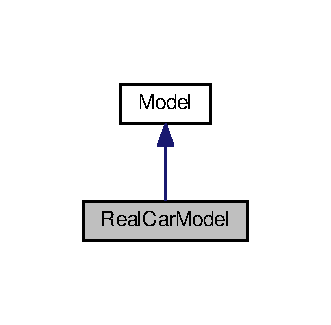
\includegraphics[width=159pt]{classRealCarModel__inherit__graph}
\end{center}
\end{figure}


Collaboration diagram for Real\+Car\+Model\+:\nopagebreak
\begin{figure}[H]
\begin{center}
\leavevmode
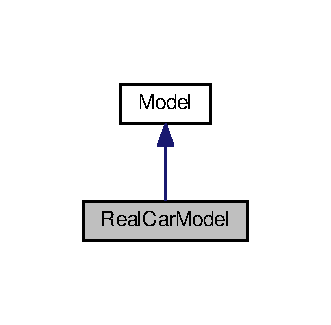
\includegraphics[width=159pt]{classRealCarModel__coll__graph}
\end{center}
\end{figure}
\subsection*{Public Member Functions}
\begin{DoxyCompactItemize}
\item 
\hyperlink{classRealCarModel_a5bb463d2448f307373b32a1f7d9254ec}{Real\+Car\+Model} ()
\item 
virtual \hyperlink{classRealCarModel_aa5e4c05702b96208a2f272d1c4cbf4e7}{$\sim$\+Real\+Car\+Model} ()
\item 
\hyperlink{Agent_8hpp_a5dd127bb3cb18b011cf5fd80a906e830}{Vector} \hyperlink{classRealCarModel_a4437d9515709862a19fdd5f7e828d757}{update} (\hyperlink{Agent_8hpp_a5dd127bb3cb18b011cf5fd80a906e830}{Vector} state, \hyperlink{Agent_8hpp_a5dd127bb3cb18b011cf5fd80a906e830}{Vector} intermediate) override
\end{DoxyCompactItemize}
\subsection*{Private Attributes}
\begin{DoxyCompactItemize}
\item 
Car\+\_\+4wheel $\ast$ \hyperlink{classRealCarModel_affb73de236aa1270f45943f35bdd2f1f}{inner\+Model}
\item 
long int \hyperlink{classRealCarModel_a808d619d7a1fa55b60ea72ccd26cc99e}{count}
\end{DoxyCompactItemize}
\subsection*{Additional Inherited Members}


\subsection{Detailed Description}
model for the real car 

\subsection{Constructor \& Destructor Documentation}
\index{Real\+Car\+Model@{Real\+Car\+Model}!Real\+Car\+Model@{Real\+Car\+Model}}
\index{Real\+Car\+Model@{Real\+Car\+Model}!Real\+Car\+Model@{Real\+Car\+Model}}
\subsubsection[{\texorpdfstring{Real\+Car\+Model()}{RealCarModel()}}]{\setlength{\rightskip}{0pt plus 5cm}Real\+Car\+Model\+::\+Real\+Car\+Model (
\begin{DoxyParamCaption}
{}
\end{DoxyParamCaption}
)\hspace{0.3cm}{\ttfamily [explicit]}}\hypertarget{classRealCarModel_a5bb463d2448f307373b32a1f7d9254ec}{}\label{classRealCarModel_a5bb463d2448f307373b32a1f7d9254ec}
Constructor. Dimension of state vector is 6 (x, y, yaw, speed x, speed y, speed yaw) Dimension of intermediate vector is 3 (proportional to gas pedal, brake pedal, and steering angle) \index{Real\+Car\+Model@{Real\+Car\+Model}!````~Real\+Car\+Model@{$\sim$\+Real\+Car\+Model}}
\index{````~Real\+Car\+Model@{$\sim$\+Real\+Car\+Model}!Real\+Car\+Model@{Real\+Car\+Model}}
\subsubsection[{\texorpdfstring{$\sim$\+Real\+Car\+Model()}{~RealCarModel()}}]{\setlength{\rightskip}{0pt plus 5cm}Real\+Car\+Model\+::$\sim$\+Real\+Car\+Model (
\begin{DoxyParamCaption}
{}
\end{DoxyParamCaption}
)\hspace{0.3cm}{\ttfamily [virtual]}}\hypertarget{classRealCarModel_aa5e4c05702b96208a2f272d1c4cbf4e7}{}\label{classRealCarModel_aa5e4c05702b96208a2f272d1c4cbf4e7}


\subsection{Member Function Documentation}
\index{Real\+Car\+Model@{Real\+Car\+Model}!update@{update}}
\index{update@{update}!Real\+Car\+Model@{Real\+Car\+Model}}
\subsubsection[{\texorpdfstring{update(\+Vector state, Vector intermediate) override}{update(Vector state, Vector intermediate) override}}]{\setlength{\rightskip}{0pt plus 5cm}{\bf Vector} Real\+Car\+Model\+::update (
\begin{DoxyParamCaption}
\item[{{\bf Vector}}]{state, }
\item[{{\bf Vector}}]{intermediate}
\end{DoxyParamCaption}
)\hspace{0.3cm}{\ttfamily [override]}, {\ttfamily [virtual]}}\hypertarget{classRealCarModel_a4437d9515709862a19fdd5f7e828d757}{}\label{classRealCarModel_a4437d9515709862a19fdd5f7e828d757}
update the state by reading .txt file 
\begin{DoxyParams}{Parameters}
{\em state} & Dimension of state vector is 6 (x, y, yaw, speed x, speed y, speed yaw). However, it doesn\textquotesingle{}t be used. \\
\hline
{\em intermediate} & Dimension of intermediate vector is 3 (proportional to gas pedal, brake pedal, and steering angle),which is empty and doesn\textquotesingle{}t be used. \\
\hline
\end{DoxyParams}
\begin{DoxyReturn}{Returns}
the state vector of this car for the next iteration 
\end{DoxyReturn}


Implements \hyperlink{classModel_a887e642d0c195b771af8300c7c817f09}{Model}.



\subsection{Member Data Documentation}
\index{Real\+Car\+Model@{Real\+Car\+Model}!count@{count}}
\index{count@{count}!Real\+Car\+Model@{Real\+Car\+Model}}
\subsubsection[{\texorpdfstring{count}{count}}]{\setlength{\rightskip}{0pt plus 5cm}long int Real\+Car\+Model\+::count\hspace{0.3cm}{\ttfamily [private]}}\hypertarget{classRealCarModel_a808d619d7a1fa55b60ea72ccd26cc99e}{}\label{classRealCarModel_a808d619d7a1fa55b60ea72ccd26cc99e}
\index{Real\+Car\+Model@{Real\+Car\+Model}!inner\+Model@{inner\+Model}}
\index{inner\+Model@{inner\+Model}!Real\+Car\+Model@{Real\+Car\+Model}}
\subsubsection[{\texorpdfstring{inner\+Model}{innerModel}}]{\setlength{\rightskip}{0pt plus 5cm}Car\+\_\+4wheel$\ast$ Real\+Car\+Model\+::inner\+Model\hspace{0.3cm}{\ttfamily [private]}}\hypertarget{classRealCarModel_affb73de236aa1270f45943f35bdd2f1f}{}\label{classRealCarModel_affb73de236aa1270f45943f35bdd2f1f}


The documentation for this class was generated from the following files\+:\begin{DoxyCompactItemize}
\item 
Models/\hyperlink{RealCarModel_8hpp}{Real\+Car\+Model.\+hpp}\item 
Models/\hyperlink{RealCarModel_8cpp}{Real\+Car\+Model.\+cpp}\end{DoxyCompactItemize}

\hypertarget{classRealCarPlanner}{}\section{Real\+Car\+Planner Class Reference}
\label{classRealCarPlanner}\index{Real\+Car\+Planner@{Real\+Car\+Planner}}


\hyperlink{classPlanner}{Planner} for the real car.  




{\ttfamily \#include $<$Real\+Car\+Planner.\+hpp$>$}



Inheritance diagram for Real\+Car\+Planner\+:\nopagebreak
\begin{figure}[H]
\begin{center}
\leavevmode
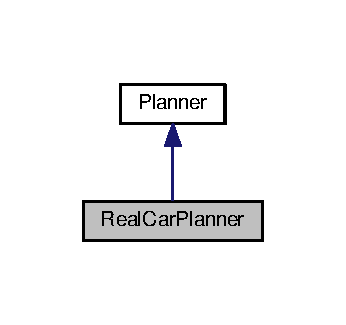
\includegraphics[width=166pt]{classRealCarPlanner__inherit__graph}
\end{center}
\end{figure}


Collaboration diagram for Real\+Car\+Planner\+:\nopagebreak
\begin{figure}[H]
\begin{center}
\leavevmode
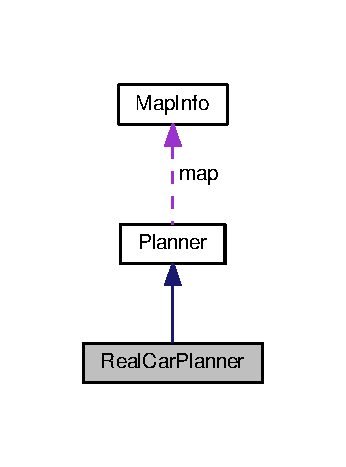
\includegraphics[width=166pt]{classRealCarPlanner__coll__graph}
\end{center}
\end{figure}
\subsection*{Public Member Functions}
\begin{DoxyCompactItemize}
\item 
\hyperlink{classRealCarPlanner_a8bf394b7d0e832e31f8f00147bf28080}{Real\+Car\+Planner} ()
\item 
\hyperlink{Agent_8hpp_a5dd127bb3cb18b011cf5fd80a906e830}{Vector} \hyperlink{classRealCarPlanner_aa7c4658f35a2310fffbd6c49474c4714}{update} (\hyperlink{Agent_8hpp_a5dd127bb3cb18b011cf5fd80a906e830}{Vector} current\+State, const \hyperlink{Agent_8hpp_a5dd127bb3cb18b011cf5fd80a906e830}{Vector} \&human\+Input, std\+::vector$<$ \hyperlink{classAgent}{Agent} $\ast$ $>$ agents) override
\end{DoxyCompactItemize}
\subsection*{Additional Inherited Members}


\subsection{Detailed Description}
\hyperlink{classPlanner}{Planner} for the real car. 

\subsection{Constructor \& Destructor Documentation}
\index{Real\+Car\+Planner@{Real\+Car\+Planner}!Real\+Car\+Planner@{Real\+Car\+Planner}}
\index{Real\+Car\+Planner@{Real\+Car\+Planner}!Real\+Car\+Planner@{Real\+Car\+Planner}}
\subsubsection[{\texorpdfstring{Real\+Car\+Planner()}{RealCarPlanner()}}]{\setlength{\rightskip}{0pt plus 5cm}Real\+Car\+Planner\+::\+Real\+Car\+Planner (
\begin{DoxyParamCaption}
{}
\end{DoxyParamCaption}
)\hspace{0.3cm}{\ttfamily [explicit]}}\hypertarget{classRealCarPlanner_a8bf394b7d0e832e31f8f00147bf28080}{}\label{classRealCarPlanner_a8bf394b7d0e832e31f8f00147bf28080}
Constructor. Dimension of state vector is 6 (x, y, yaw, speed x, speed y, speed yaw) Dimension of input vector is 3 (gas pedal, brake pedal, and steering angle) 

\subsection{Member Function Documentation}
\index{Real\+Car\+Planner@{Real\+Car\+Planner}!update@{update}}
\index{update@{update}!Real\+Car\+Planner@{Real\+Car\+Planner}}
\subsubsection[{\texorpdfstring{update(\+Vector current\+State, const Vector \&human\+Input, std\+::vector$<$ Agent $\ast$ $>$ agents) override}{update(Vector currentState, const Vector &humanInput, std::vector< Agent * > agents) override}}]{\setlength{\rightskip}{0pt plus 5cm}{\bf Vector} Real\+Car\+Planner\+::update (
\begin{DoxyParamCaption}
\item[{{\bf Vector}}]{current\+State, }
\item[{const {\bf Vector} \&}]{human\+Input, }
\item[{std\+::vector$<$ {\bf Agent} $\ast$ $>$}]{agents}
\end{DoxyParamCaption}
)\hspace{0.3cm}{\ttfamily [override]}, {\ttfamily [virtual]}}\hypertarget{classRealCarPlanner_aa7c4658f35a2310fffbd6c49474c4714}{}\label{classRealCarPlanner_aa7c4658f35a2310fffbd6c49474c4714}
just returen a empty vector,since the real car\textquotesingle{}s state is coming form the real world. 
\begin{DoxyParams}{Parameters}
{\em current\+State} & current state of the car. Doesn\textquotesingle{}t be used \\
\hline
{\em human\+Input} & current human input vector (gas pedal, brake pedal, and steering angle). Empty and doesn\textquotesingle{}t be used \\
\hline
{\em agents} & information of all agents in the simulator. Doesn\textquotesingle{}t be used \\
\hline
\end{DoxyParams}
\begin{DoxyReturn}{Returns}
empty vector,since the real car\textquotesingle{}s state is coming form the real world. 
\end{DoxyReturn}


Implements \hyperlink{classPlanner_a62e1434402a3f36b0883e069a10447d8}{Planner}.



The documentation for this class was generated from the following files\+:\begin{DoxyCompactItemize}
\item 
Planners/\hyperlink{RealCarPlanner_8hpp}{Real\+Car\+Planner.\+hpp}\item 
Planners/\hyperlink{RealCarPlanner_8cpp}{Real\+Car\+Planner.\+cpp}\end{DoxyCompactItemize}

\hypertarget{classServer}{}\section{Server Class Reference}
\label{classServer}\index{Server@{Server}}


The class of all server using rpclib.  




{\ttfamily \#include $<$Server.\+hpp$>$}



Collaboration diagram for Server\+:\nopagebreak
\begin{figure}[H]
\begin{center}
\leavevmode
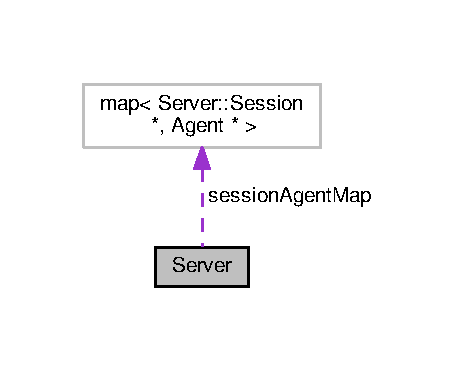
\includegraphics[width=219pt]{classServer__coll__graph}
\end{center}
\end{figure}
\subsection*{Classes}
\begin{DoxyCompactItemize}
\item 
struct \hyperlink{structServer_1_1Session}{Session}
\begin{DoxyCompactList}\small\item\em An structure for session including session id and its type. \end{DoxyCompactList}\end{DoxyCompactItemize}
\subsection*{Public Member Functions}
\begin{DoxyCompactItemize}
\item 
\hyperlink{classServer_a574f6493828dccb18a0ca6a86ee7dfa4}{Server} (int port, \hyperlink{main_8hpp_a4cb9f4bcd812094244f1949a88671bb8}{Simulator\+State} \&\hyperlink{classServer_a1e6a901e88f3a8b2d2fea253e32952e4}{simulator\+State}, \hyperlink{Server_8hpp_a49cc8333bde52a7f1eb36bdb3e4e8a06}{Input\+Dictionary} \&\hyperlink{classServer_a3d62b0bc3c31161790b118717a4c4718}{human\+Inputs}, \hyperlink{Server_8hpp_acc6d6e73aa06631da7c2f627f9979d64}{Agent\+Dictionary} \&\hyperlink{classServer_ae45bd58f8585e0c47e5140a055cad09c}{agent\+Dictionary}, std\+::mutex \&\hyperlink{classServer_a9a508fe15f3a6e3b2e3750b0ff2d5798}{mutex})
\end{DoxyCompactItemize}
\subsection*{Private Types}
\begin{DoxyCompactItemize}
\item 
enum \hyperlink{classServer_abb49932aed3c7683040e1a463e25c36c}{Session\+Type} \{ \hyperlink{classServer_abb49932aed3c7683040e1a463e25c36ca5927e9d71a6843a513199c25c2c62f82}{Rendering} = 0, 
\hyperlink{classServer_abb49932aed3c7683040e1a463e25c36cae387e75adf857bbe8390734f939efbdf}{Input} = 1
 \}
\item 
typedef std\+::pair$<$ \hyperlink{structServer_1_1Session}{Session} $\ast$, \hyperlink{classAgent}{Agent} $\ast$ $>$ \hyperlink{classServer_a5b3a89ca943df0f41fdf902a0c2147f3}{Session\+Agent\+Pair}
\end{DoxyCompactItemize}
\subsection*{Private Member Functions}
\begin{DoxyCompactItemize}
\item 
string \hyperlink{classServer_a075ea5a350e5b6052dc621411526e469}{respond\+Manager} (const string \&request\+Json)
\item 
string \hyperlink{classServer_ad542ec541766a9524fcf7d4569699c4e}{respond\+Rendering} (const string \&request\+Json)
\item 
string \hyperlink{classServer_a908709257a0191b87ac66aa509d11140}{respond\+Input} (const string \&request\+Json)
\item 
Json\+::\+Value \hyperlink{classServer_a76481ef963d4dc3478b72edd1c164f7a}{get\+Session\+Info} (bool with\+Lock=true) const 
\item 
Json\+::\+Value \hyperlink{classServer_a7c116bd269521368538c5d4836b43f9b}{get\+Agent\+Info} (bool with\+Lock=true) const 
\item 
\hyperlink{classAgent}{Agent} $\ast$ \hyperlink{classServer_a8def8e7ae4ee50c38c612e6ded9f9c94}{find\+Agent\+By\+Id} (int id) const 
\item 
\hyperlink{structServer_1_1Session}{Session} $\ast$ \hyperlink{classServer_ad43e988ffc6fb0398db3191309ff0eee}{find\+Session\+By\+Id} (int id) const 
\end{DoxyCompactItemize}
\subsection*{Static Private Member Functions}
\begin{DoxyCompactItemize}
\item 
static \hyperlink{Agent_8hpp_a5dd127bb3cb18b011cf5fd80a906e830}{Vector} \hyperlink{classServer_af46e68595c4f0729d5cb4f72f4fd6e28}{Json2\+Vector} (const Json\+::\+Value \&val)
\item 
static Json\+::\+Value \hyperlink{classServer_ae58496ca71e4c467209c98ac1af02994}{Vector2\+Json} (const \hyperlink{Agent_8hpp_a5dd127bb3cb18b011cf5fd80a906e830}{Vector} \&vec)
\end{DoxyCompactItemize}
\subsection*{Private Attributes}
\begin{DoxyCompactItemize}
\item 
rpc\+::server \hyperlink{classServer_a3f6f17fe0e321f0e4fc6bed80a5efc3d}{server}
\item 
\hyperlink{main_8hpp_a4cb9f4bcd812094244f1949a88671bb8}{Simulator\+State} \& \hyperlink{classServer_a1e6a901e88f3a8b2d2fea253e32952e4}{simulator\+State}
\item 
\hyperlink{Server_8hpp_acc6d6e73aa06631da7c2f627f9979d64}{Agent\+Dictionary} \& \hyperlink{classServer_ae45bd58f8585e0c47e5140a055cad09c}{agent\+Dictionary}
\item 
std\+::mutex \& \hyperlink{classServer_a9a508fe15f3a6e3b2e3750b0ff2d5798}{mutex}
\item 
\hyperlink{Server_8hpp_a49cc8333bde52a7f1eb36bdb3e4e8a06}{Input\+Dictionary} \& \hyperlink{classServer_a3d62b0bc3c31161790b118717a4c4718}{human\+Inputs}
\item 
map$<$ \hyperlink{structServer_1_1Session}{Session} $\ast$, \hyperlink{classAgent}{Agent} $\ast$ $>$ \hyperlink{classServer_ad19c76785348bfd91a941aa78ef6a35c}{session\+Agent\+Map}
\item 
int \hyperlink{classServer_ac179860cef2427f743ff1daefa881eb2}{agent\+Id\+Counter}
\item 
int \hyperlink{classServer_abcdb8b5ca33795cdd8f252cf4c3e4f0f}{session\+Id\+Counter}
\end{DoxyCompactItemize}


\subsection{Detailed Description}
The class of all server using rpclib. 

It have three kinds of services for input, manager and rendering. 

\subsection{Member Typedef Documentation}
\index{Server@{Server}!Session\+Agent\+Pair@{Session\+Agent\+Pair}}
\index{Session\+Agent\+Pair@{Session\+Agent\+Pair}!Server@{Server}}
\subsubsection[{\texorpdfstring{Session\+Agent\+Pair}{SessionAgentPair}}]{\setlength{\rightskip}{0pt plus 5cm}typedef std\+::pair$<${\bf Session}$\ast$, {\bf Agent}$\ast$$>$ {\bf Server\+::\+Session\+Agent\+Pair}\hspace{0.3cm}{\ttfamily [private]}}\hypertarget{classServer_a5b3a89ca943df0f41fdf902a0c2147f3}{}\label{classServer_a5b3a89ca943df0f41fdf902a0c2147f3}


\subsection{Member Enumeration Documentation}
\index{Server@{Server}!Session\+Type@{Session\+Type}}
\index{Session\+Type@{Session\+Type}!Server@{Server}}
\subsubsection[{\texorpdfstring{Session\+Type}{SessionType}}]{\setlength{\rightskip}{0pt plus 5cm}enum {\bf Server\+::\+Session\+Type}\hspace{0.3cm}{\ttfamily [private]}}\hypertarget{classServer_abb49932aed3c7683040e1a463e25c36c}{}\label{classServer_abb49932aed3c7683040e1a463e25c36c}
An enum type It represent to the session type. \begin{Desc}
\item[Enumerator]\par
\begin{description}
\index{Rendering@{Rendering}!Server@{Server}}\index{Server@{Server}!Rendering@{Rendering}}\item[{\em 
Rendering\hypertarget{classServer_abb49932aed3c7683040e1a463e25c36ca5927e9d71a6843a513199c25c2c62f82}{}\label{classServer_abb49932aed3c7683040e1a463e25c36ca5927e9d71a6843a513199c25c2c62f82}
}]\index{Input@{Input}!Server@{Server}}\index{Server@{Server}!Input@{Input}}\item[{\em 
Input\hypertarget{classServer_abb49932aed3c7683040e1a463e25c36cae387e75adf857bbe8390734f939efbdf}{}\label{classServer_abb49932aed3c7683040e1a463e25c36cae387e75adf857bbe8390734f939efbdf}
}]\end{description}
\end{Desc}


\subsection{Constructor \& Destructor Documentation}
\index{Server@{Server}!Server@{Server}}
\index{Server@{Server}!Server@{Server}}
\subsubsection[{\texorpdfstring{Server(int port, Simulator\+State \&simulator\+State, Input\+Dictionary \&human\+Inputs, Agent\+Dictionary \&agent\+Dictionary, std\+::mutex \&mutex)}{Server(int port, SimulatorState &simulatorState, InputDictionary &humanInputs, AgentDictionary &agentDictionary, std::mutex &mutex)}}]{\setlength{\rightskip}{0pt plus 5cm}Server\+::\+Server (
\begin{DoxyParamCaption}
\item[{int}]{port, }
\item[{{\bf Simulator\+State} \&}]{simulator\+State, }
\item[{{\bf Input\+Dictionary} \&}]{human\+Inputs, }
\item[{{\bf Agent\+Dictionary} \&}]{agent\+Dictionary, }
\item[{std\+::mutex \&}]{mutex}
\end{DoxyParamCaption}
)}\hypertarget{classServer_a574f6493828dccb18a0ca6a86ee7dfa4}{}\label{classServer_a574f6493828dccb18a0ca6a86ee7dfa4}
Constructor. 
\begin{DoxyParams}{Parameters}
{\em port} & port for simulation. \\
\hline
{\em simulator\+State} & reference to the simulator state, an enumerator. \\
\hline
{\em human\+Inputs} & reference to a map from agent to pertaining vector human input. \\
\hline
{\em agent\+Dictionary} & reference to a map from agent to pertaining controller, model, and planner. \\
\hline
{\em mutex} & reference to a global mutex lock, which avoids thread conflicts. \\
\hline
\end{DoxyParams}


\subsection{Member Function Documentation}
\index{Server@{Server}!find\+Agent\+By\+Id@{find\+Agent\+By\+Id}}
\index{find\+Agent\+By\+Id@{find\+Agent\+By\+Id}!Server@{Server}}
\subsubsection[{\texorpdfstring{find\+Agent\+By\+Id(int id) const }{findAgentById(int id) const }}]{\setlength{\rightskip}{0pt plus 5cm}{\bf Agent} $\ast$ Server\+::find\+Agent\+By\+Id (
\begin{DoxyParamCaption}
\item[{int}]{id}
\end{DoxyParamCaption}
) const\hspace{0.3cm}{\ttfamily [private]}}\hypertarget{classServer_a8def8e7ae4ee50c38c612e6ded9f9c94}{}\label{classServer_a8def8e7ae4ee50c38c612e6ded9f9c94}
Find an agent in the simulator by its id. 
\begin{DoxyParams}{Parameters}
{\em id} & id of the agent to find \\
\hline
\end{DoxyParams}
\begin{DoxyReturn}{Returns}
pointer to that agent 
\end{DoxyReturn}
\index{Server@{Server}!find\+Session\+By\+Id@{find\+Session\+By\+Id}}
\index{find\+Session\+By\+Id@{find\+Session\+By\+Id}!Server@{Server}}
\subsubsection[{\texorpdfstring{find\+Session\+By\+Id(int id) const }{findSessionById(int id) const }}]{\setlength{\rightskip}{0pt plus 5cm}{\bf Server\+::\+Session} $\ast$ Server\+::find\+Session\+By\+Id (
\begin{DoxyParamCaption}
\item[{int}]{id}
\end{DoxyParamCaption}
) const\hspace{0.3cm}{\ttfamily [private]}}\hypertarget{classServer_ad43e988ffc6fb0398db3191309ff0eee}{}\label{classServer_ad43e988ffc6fb0398db3191309ff0eee}
Find a session in the simulator by its id. \hyperlink{structServer_1_1Session}{Session} is an abstraction of a connection socket to a client. 
\begin{DoxyParams}{Parameters}
{\em id} & id of the session to find \\
\hline
\end{DoxyParams}
\begin{DoxyReturn}{Returns}
pointer to that session 
\end{DoxyReturn}
\index{Server@{Server}!get\+Agent\+Info@{get\+Agent\+Info}}
\index{get\+Agent\+Info@{get\+Agent\+Info}!Server@{Server}}
\subsubsection[{\texorpdfstring{get\+Agent\+Info(bool with\+Lock=true) const }{getAgentInfo(bool withLock=true) const }}]{\setlength{\rightskip}{0pt plus 5cm}Json\+::\+Value Server\+::get\+Agent\+Info (
\begin{DoxyParamCaption}
\item[{bool}]{with\+Lock = {\ttfamily true}}
\end{DoxyParamCaption}
) const\hspace{0.3cm}{\ttfamily [private]}}\hypertarget{classServer_a7c116bd269521368538c5d4836b43f9b}{}\label{classServer_a7c116bd269521368538c5d4836b43f9b}
Get the information of all agents in the simulator 
\begin{DoxyParams}{Parameters}
{\em with\+Lock} & should use mutex lock or not \\
\hline
\end{DoxyParams}
\begin{DoxyReturn}{Returns}
agent information serialized in Json format 
\end{DoxyReturn}
\index{Server@{Server}!get\+Session\+Info@{get\+Session\+Info}}
\index{get\+Session\+Info@{get\+Session\+Info}!Server@{Server}}
\subsubsection[{\texorpdfstring{get\+Session\+Info(bool with\+Lock=true) const }{getSessionInfo(bool withLock=true) const }}]{\setlength{\rightskip}{0pt plus 5cm}Json\+::\+Value Server\+::get\+Session\+Info (
\begin{DoxyParamCaption}
\item[{bool}]{with\+Lock = {\ttfamily true}}
\end{DoxyParamCaption}
) const\hspace{0.3cm}{\ttfamily [private]}}\hypertarget{classServer_a76481ef963d4dc3478b72edd1c164f7a}{}\label{classServer_a76481ef963d4dc3478b72edd1c164f7a}
Get the information of all sessions in the simulator 
\begin{DoxyParams}{Parameters}
{\em with\+Lock} & should use mutex lock or not \\
\hline
\end{DoxyParams}
\begin{DoxyReturn}{Returns}
agent information serialized in Json format 
\end{DoxyReturn}
\index{Server@{Server}!Json2\+Vector@{Json2\+Vector}}
\index{Json2\+Vector@{Json2\+Vector}!Server@{Server}}
\subsubsection[{\texorpdfstring{Json2\+Vector(const Json\+::\+Value \&val)}{Json2Vector(const Json::Value &val)}}]{\setlength{\rightskip}{0pt plus 5cm}{\bf Vector} Server\+::\+Json2\+Vector (
\begin{DoxyParamCaption}
\item[{const Json\+::\+Value \&}]{val}
\end{DoxyParamCaption}
)\hspace{0.3cm}{\ttfamily [static]}, {\ttfamily [private]}}\hypertarget{classServer_af46e68595c4f0729d5cb4f72f4fd6e28}{}\label{classServer_af46e68595c4f0729d5cb4f72f4fd6e28}
Convert a std\+::vector$<$double$>$ to a Json\+::\+Value 
\begin{DoxyParams}{Parameters}
{\em val} & a json value (defined in jsoncpp library) \\
\hline
\end{DoxyParams}
\begin{DoxyReturn}{Returns}
a S\+TL vector 
\end{DoxyReturn}
\index{Server@{Server}!respond\+Input@{respond\+Input}}
\index{respond\+Input@{respond\+Input}!Server@{Server}}
\subsubsection[{\texorpdfstring{respond\+Input(const string \&request\+Json)}{respondInput(const string &requestJson)}}]{\setlength{\rightskip}{0pt plus 5cm}string Server\+::respond\+Input (
\begin{DoxyParamCaption}
\item[{const string \&}]{request\+Json}
\end{DoxyParamCaption}
)\hspace{0.3cm}{\ttfamily [private]}}\hypertarget{classServer_a908709257a0191b87ac66aa509d11140}{}\label{classServer_a908709257a0191b87ac66aa509d11140}
Respond to a request from a client for input hardware it have two commands\+: \char`\"{}new\+Session\char`\"{} if the client connects for the first time, and requests a new session. \char`\"{}update\+Input\char`\"{} if the client already has a session, and updates the input vector. 
\begin{DoxyParams}{Parameters}
{\em request\+Json} & request string in Json format \\
\hline
\end{DoxyParams}
\begin{DoxyReturn}{Returns}
response string in Json format 
\end{DoxyReturn}
\index{Server@{Server}!respond\+Manager@{respond\+Manager}}
\index{respond\+Manager@{respond\+Manager}!Server@{Server}}
\subsubsection[{\texorpdfstring{respond\+Manager(const string \&request\+Json)}{respondManager(const string &requestJson)}}]{\setlength{\rightskip}{0pt plus 5cm}string Server\+::respond\+Manager (
\begin{DoxyParamCaption}
\item[{const string \&}]{request\+Json}
\end{DoxyParamCaption}
)\hspace{0.3cm}{\ttfamily [private]}}\hypertarget{classServer_a075ea5a350e5b6052dc621411526e469}{}\label{classServer_a075ea5a350e5b6052dc621411526e469}
Respond to a request from a manager client, who controls the simulator server. it have various command\+: \char`\"{}pause\char`\"{} \char`\"{}start\char`\"{} \char`\"{}reset\char`\"{} if the manager wants to change the state of the simulator. \char`\"{}startvc\char`\"{} if the manager wants to add the virtual car into the simulator. \char`\"{}get\+Agents\char`\"{} \char`\"{}get\+Sessions\char`\"{} if the manager wants to get information of all agents or all sessions. \char`\"{}get\+Times\char`\"{} if the manager wants to get the times that the simulator have updated. \char`\"{}get\+Time\char`\"{} if the manager wants to get the time that the simulator cost for last updating state. \char`\"{}add\+Agent\char`\"{} if the manager wants to add an agent dynamically.. \char`\"{}bind\+Agent\+To\+Session\char`\"{} if the manager wants to bind an agent to a session dynamically. 
\begin{DoxyParams}{Parameters}
{\em request\+Json} & request string in Json format \\
\hline
\end{DoxyParams}
\begin{DoxyReturn}{Returns}
response string in Json format 
\end{DoxyReturn}
\index{Server@{Server}!respond\+Rendering@{respond\+Rendering}}
\index{respond\+Rendering@{respond\+Rendering}!Server@{Server}}
\subsubsection[{\texorpdfstring{respond\+Rendering(const string \&request\+Json)}{respondRendering(const string &requestJson)}}]{\setlength{\rightskip}{0pt plus 5cm}string Server\+::respond\+Rendering (
\begin{DoxyParamCaption}
\item[{const string \&}]{request\+Json}
\end{DoxyParamCaption}
)\hspace{0.3cm}{\ttfamily [private]}}\hypertarget{classServer_ad542ec541766a9524fcf7d4569699c4e}{}\label{classServer_ad542ec541766a9524fcf7d4569699c4e}
Respond to a request from a client for rendering in U\+E4 it have two commands\+: \char`\"{}new\+Session\char`\"{} if the client connects for the first time, and requests a new session. \char`\"{}get\+Agents\char`\"{} if the client already has a session, and gets the agent information. 
\begin{DoxyParams}{Parameters}
{\em request\+Json} & request string in Json format \\
\hline
\end{DoxyParams}
\begin{DoxyReturn}{Returns}
response string in Json format 
\end{DoxyReturn}
\index{Server@{Server}!Vector2\+Json@{Vector2\+Json}}
\index{Vector2\+Json@{Vector2\+Json}!Server@{Server}}
\subsubsection[{\texorpdfstring{Vector2\+Json(const Vector \&vec)}{Vector2Json(const Vector &vec)}}]{\setlength{\rightskip}{0pt plus 5cm}Json\+::\+Value Server\+::\+Vector2\+Json (
\begin{DoxyParamCaption}
\item[{const {\bf Vector} \&}]{vec}
\end{DoxyParamCaption}
)\hspace{0.3cm}{\ttfamily [static]}, {\ttfamily [private]}}\hypertarget{classServer_ae58496ca71e4c467209c98ac1af02994}{}\label{classServer_ae58496ca71e4c467209c98ac1af02994}
Convert a Json\+::\+Value to a std\+::vector 
\begin{DoxyParams}{Parameters}
{\em vec} & a S\+TL vector \\
\hline
\end{DoxyParams}
\begin{DoxyReturn}{Returns}
a json value (defined in jsoncpp library) 
\end{DoxyReturn}


\subsection{Member Data Documentation}
\index{Server@{Server}!agent\+Dictionary@{agent\+Dictionary}}
\index{agent\+Dictionary@{agent\+Dictionary}!Server@{Server}}
\subsubsection[{\texorpdfstring{agent\+Dictionary}{agentDictionary}}]{\setlength{\rightskip}{0pt plus 5cm}{\bf Agent\+Dictionary}\& Server\+::agent\+Dictionary\hspace{0.3cm}{\ttfamily [private]}}\hypertarget{classServer_ae45bd58f8585e0c47e5140a055cad09c}{}\label{classServer_ae45bd58f8585e0c47e5140a055cad09c}
reference to a map from agent to pertaining controller, model, and planner. \index{Server@{Server}!agent\+Id\+Counter@{agent\+Id\+Counter}}
\index{agent\+Id\+Counter@{agent\+Id\+Counter}!Server@{Server}}
\subsubsection[{\texorpdfstring{agent\+Id\+Counter}{agentIdCounter}}]{\setlength{\rightskip}{0pt plus 5cm}int Server\+::agent\+Id\+Counter\hspace{0.3cm}{\ttfamily [private]}}\hypertarget{classServer_ac179860cef2427f743ff1daefa881eb2}{}\label{classServer_ac179860cef2427f743ff1daefa881eb2}
an counter for agent to get different id for agents \index{Server@{Server}!human\+Inputs@{human\+Inputs}}
\index{human\+Inputs@{human\+Inputs}!Server@{Server}}
\subsubsection[{\texorpdfstring{human\+Inputs}{humanInputs}}]{\setlength{\rightskip}{0pt plus 5cm}{\bf Input\+Dictionary}\& Server\+::human\+Inputs\hspace{0.3cm}{\ttfamily [private]}}\hypertarget{classServer_a3d62b0bc3c31161790b118717a4c4718}{}\label{classServer_a3d62b0bc3c31161790b118717a4c4718}
reference to a map from agent to pertaining vector human input. \index{Server@{Server}!mutex@{mutex}}
\index{mutex@{mutex}!Server@{Server}}
\subsubsection[{\texorpdfstring{mutex}{mutex}}]{\setlength{\rightskip}{0pt plus 5cm}std\+::mutex\& Server\+::mutex\hspace{0.3cm}{\ttfamily [private]}}\hypertarget{classServer_a9a508fe15f3a6e3b2e3750b0ff2d5798}{}\label{classServer_a9a508fe15f3a6e3b2e3750b0ff2d5798}
reference to a global mutex lock, which avoids thread conflicts. \index{Server@{Server}!server@{server}}
\index{server@{server}!Server@{Server}}
\subsubsection[{\texorpdfstring{server}{server}}]{\setlength{\rightskip}{0pt plus 5cm}rpc\+::server Server\+::server\hspace{0.3cm}{\ttfamily [private]}}\hypertarget{classServer_a3f6f17fe0e321f0e4fc6bed80a5efc3d}{}\label{classServer_a3f6f17fe0e321f0e4fc6bed80a5efc3d}
server of rpclib \index{Server@{Server}!session\+Agent\+Map@{session\+Agent\+Map}}
\index{session\+Agent\+Map@{session\+Agent\+Map}!Server@{Server}}
\subsubsection[{\texorpdfstring{session\+Agent\+Map}{sessionAgentMap}}]{\setlength{\rightskip}{0pt plus 5cm}map$<${\bf Session}$\ast$, {\bf Agent}$\ast$$>$ Server\+::session\+Agent\+Map\hspace{0.3cm}{\ttfamily [private]}}\hypertarget{classServer_ad19c76785348bfd91a941aa78ef6a35c}{}\label{classServer_ad19c76785348bfd91a941aa78ef6a35c}
\index{Server@{Server}!session\+Id\+Counter@{session\+Id\+Counter}}
\index{session\+Id\+Counter@{session\+Id\+Counter}!Server@{Server}}
\subsubsection[{\texorpdfstring{session\+Id\+Counter}{sessionIdCounter}}]{\setlength{\rightskip}{0pt plus 5cm}int Server\+::session\+Id\+Counter\hspace{0.3cm}{\ttfamily [private]}}\hypertarget{classServer_abcdb8b5ca33795cdd8f252cf4c3e4f0f}{}\label{classServer_abcdb8b5ca33795cdd8f252cf4c3e4f0f}
an counter for session to get different id for session \index{Server@{Server}!simulator\+State@{simulator\+State}}
\index{simulator\+State@{simulator\+State}!Server@{Server}}
\subsubsection[{\texorpdfstring{simulator\+State}{simulatorState}}]{\setlength{\rightskip}{0pt plus 5cm}{\bf Simulator\+State}\& Server\+::simulator\+State\hspace{0.3cm}{\ttfamily [private]}}\hypertarget{classServer_a1e6a901e88f3a8b2d2fea253e32952e4}{}\label{classServer_a1e6a901e88f3a8b2d2fea253e32952e4}
reference to the simulator state, an enumerator. 

The documentation for this class was generated from the following files\+:\begin{DoxyCompactItemize}
\item 
Server/\hyperlink{Server_8hpp}{Server.\+hpp}\item 
Server/\hyperlink{Server_8cpp}{Server.\+cpp}\item 
Server/\hyperlink{ServerRespondInput_8cpp}{Server\+Respond\+Input.\+cpp}\item 
Server/\hyperlink{ServerRespondManager_8cpp}{Server\+Respond\+Manager.\+cpp}\item 
Server/\hyperlink{ServerRespondRendering_8cpp}{Server\+Respond\+Rendering.\+cpp}\end{DoxyCompactItemize}

\hypertarget{structServer_1_1Session}{}\section{Server\+:\+:Session Struct Reference}
\label{structServer_1_1Session}\index{Server\+::\+Session@{Server\+::\+Session}}


An structure for session including session id and its type.  


\subsection*{Public Attributes}
\begin{DoxyCompactItemize}
\item 
int \hyperlink{structServer_1_1Session_adb3fcb9d4bb8f7bd102d16ac3ba1f434}{session\+Id}
\item 
\hyperlink{classServer_abb49932aed3c7683040e1a463e25c36c}{Session\+Type} \hyperlink{structServer_1_1Session_a3d598a0da58b1882678cb4e2d9712611}{session\+Type}
\end{DoxyCompactItemize}


\subsection{Detailed Description}
An structure for session including session id and its type. 

\subsection{Member Data Documentation}
\index{Server\+::\+Session@{Server\+::\+Session}!session\+Id@{session\+Id}}
\index{session\+Id@{session\+Id}!Server\+::\+Session@{Server\+::\+Session}}
\subsubsection[{\texorpdfstring{session\+Id}{sessionId}}]{\setlength{\rightskip}{0pt plus 5cm}int Server\+::\+Session\+::session\+Id}\hypertarget{structServer_1_1Session_adb3fcb9d4bb8f7bd102d16ac3ba1f434}{}\label{structServer_1_1Session_adb3fcb9d4bb8f7bd102d16ac3ba1f434}
\index{Server\+::\+Session@{Server\+::\+Session}!session\+Type@{session\+Type}}
\index{session\+Type@{session\+Type}!Server\+::\+Session@{Server\+::\+Session}}
\subsubsection[{\texorpdfstring{session\+Type}{sessionType}}]{\setlength{\rightskip}{0pt plus 5cm}{\bf Session\+Type} Server\+::\+Session\+::session\+Type}\hypertarget{structServer_1_1Session_a3d598a0da58b1882678cb4e2d9712611}{}\label{structServer_1_1Session_a3d598a0da58b1882678cb4e2d9712611}


The documentation for this struct was generated from the following file\+:\begin{DoxyCompactItemize}
\item 
Server/\hyperlink{Server_8hpp}{Server.\+hpp}\end{DoxyCompactItemize}

\hypertarget{classSimplePidController}{}\section{Simple\+Pid\+Controller Class Reference}
\label{classSimplePidController}\index{Simple\+Pid\+Controller@{Simple\+Pid\+Controller}}


A Simple\+Pid controller is the controller for the \hyperlink{classPlanner}{Planner} which may plan many step.  




{\ttfamily \#include $<$Simple\+Pid\+Controller.\+hpp$>$}



Inheritance diagram for Simple\+Pid\+Controller\+:\nopagebreak
\begin{figure}[H]
\begin{center}
\leavevmode
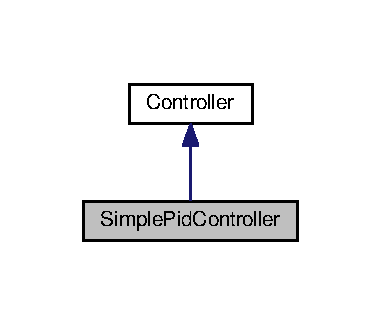
\includegraphics[width=183pt]{classSimplePidController__inherit__graph}
\end{center}
\end{figure}


Collaboration diagram for Simple\+Pid\+Controller\+:\nopagebreak
\begin{figure}[H]
\begin{center}
\leavevmode
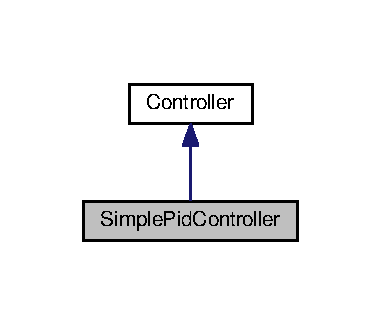
\includegraphics[width=183pt]{classSimplePidController__coll__graph}
\end{center}
\end{figure}
\subsection*{Public Member Functions}
\begin{DoxyCompactItemize}
\item 
\hyperlink{classSimplePidController_a0474257f1519261f378c4dbbf6aae991}{Simple\+Pid\+Controller} ()
\item 
virtual \hyperlink{classSimplePidController_a73681b7f58dd0dc94999f225530aa9f9}{$\sim$\+Simple\+Pid\+Controller} ()
\item 
\hyperlink{Agent_8hpp_a5dd127bb3cb18b011cf5fd80a906e830}{Vector} \hyperlink{classSimplePidController_ae849967e635ea1c6237f614d08156931}{update} (\hyperlink{Agent_8hpp_a5dd127bb3cb18b011cf5fd80a906e830}{Vector} input) override
\end{DoxyCompactItemize}
\subsection*{Protected Attributes}
\begin{DoxyCompactItemize}
\item 
Pid\+Controller $\ast$ \hyperlink{classSimplePidController_ab46e7126d3eb60e4f492de4f6da051e2}{inner\+Controller}
\end{DoxyCompactItemize}


\subsection{Detailed Description}
A Simple\+Pid controller is the controller for the \hyperlink{classPlanner}{Planner} which may plan many step. 

\subsection{Constructor \& Destructor Documentation}
\index{Simple\+Pid\+Controller@{Simple\+Pid\+Controller}!Simple\+Pid\+Controller@{Simple\+Pid\+Controller}}
\index{Simple\+Pid\+Controller@{Simple\+Pid\+Controller}!Simple\+Pid\+Controller@{Simple\+Pid\+Controller}}
\subsubsection[{\texorpdfstring{Simple\+Pid\+Controller()}{SimplePidController()}}]{\setlength{\rightskip}{0pt plus 5cm}Simple\+Pid\+Controller\+::\+Simple\+Pid\+Controller (
\begin{DoxyParamCaption}
{}
\end{DoxyParamCaption}
)\hspace{0.3cm}{\ttfamily [explicit]}}\hypertarget{classSimplePidController_a0474257f1519261f378c4dbbf6aae991}{}\label{classSimplePidController_a0474257f1519261f378c4dbbf6aae991}
Constructor. Dimension of input vector is 6 + 4 $\ast$ P\+L\+A\+N\+\_\+\+S\+T\+EP (current state and P\+L\+A\+N\+\_\+\+S\+T\+EP state(t, x , y, v) that want to follow) Dimension of intermediate vector is 3. \index{Simple\+Pid\+Controller@{Simple\+Pid\+Controller}!````~Simple\+Pid\+Controller@{$\sim$\+Simple\+Pid\+Controller}}
\index{````~Simple\+Pid\+Controller@{$\sim$\+Simple\+Pid\+Controller}!Simple\+Pid\+Controller@{Simple\+Pid\+Controller}}
\subsubsection[{\texorpdfstring{$\sim$\+Simple\+Pid\+Controller()}{~SimplePidController()}}]{\setlength{\rightskip}{0pt plus 5cm}Simple\+Pid\+Controller\+::$\sim$\+Simple\+Pid\+Controller (
\begin{DoxyParamCaption}
{}
\end{DoxyParamCaption}
)\hspace{0.3cm}{\ttfamily [virtual]}}\hypertarget{classSimplePidController_a73681b7f58dd0dc94999f225530aa9f9}{}\label{classSimplePidController_a73681b7f58dd0dc94999f225530aa9f9}


\subsection{Member Function Documentation}
\index{Simple\+Pid\+Controller@{Simple\+Pid\+Controller}!update@{update}}
\index{update@{update}!Simple\+Pid\+Controller@{Simple\+Pid\+Controller}}
\subsubsection[{\texorpdfstring{update(\+Vector input) override}{update(Vector input) override}}]{\setlength{\rightskip}{0pt plus 5cm}{\bf Vector} Simple\+Pid\+Controller\+::update (
\begin{DoxyParamCaption}
\item[{{\bf Vector}}]{input}
\end{DoxyParamCaption}
)\hspace{0.3cm}{\ttfamily [override]}, {\ttfamily [virtual]}}\hypertarget{classSimplePidController_ae849967e635ea1c6237f614d08156931}{}\label{classSimplePidController_ae849967e635ea1c6237f614d08156931}
Proportional controller. 
\begin{DoxyParams}{Parameters}
{\em input} & input vector (current state and P\+L\+A\+N\+\_\+\+S\+T\+EP state(t, x , y, v) that want to follow) \\
\hline
\end{DoxyParams}
\begin{DoxyReturn}{Returns}
intermediate vector. 
\end{DoxyReturn}


Implements \hyperlink{classController_acef11e408fb0d66d272bf5ab828cfbf6}{Controller}.



\subsection{Member Data Documentation}
\index{Simple\+Pid\+Controller@{Simple\+Pid\+Controller}!inner\+Controller@{inner\+Controller}}
\index{inner\+Controller@{inner\+Controller}!Simple\+Pid\+Controller@{Simple\+Pid\+Controller}}
\subsubsection[{\texorpdfstring{inner\+Controller}{innerController}}]{\setlength{\rightskip}{0pt plus 5cm}Pid\+Controller$\ast$ Simple\+Pid\+Controller\+::inner\+Controller\hspace{0.3cm}{\ttfamily [protected]}}\hypertarget{classSimplePidController_ab46e7126d3eb60e4f492de4f6da051e2}{}\label{classSimplePidController_ab46e7126d3eb60e4f492de4f6da051e2}


The documentation for this class was generated from the following files\+:\begin{DoxyCompactItemize}
\item 
Controllers/\hyperlink{SimplePidController_8hpp}{Simple\+Pid\+Controller.\+hpp}\item 
Controllers/\hyperlink{SimplePidController_8cpp}{Simple\+Pid\+Controller.\+cpp}\end{DoxyCompactItemize}

\hypertarget{classSimulator}{}\section{Simulator Class Reference}
\label{classSimulator}\index{Simulator@{Simulator}}


The class of the whole simulator.  




{\ttfamily \#include $<$Simulator.\+hpp$>$}



Collaboration diagram for Simulator\+:\nopagebreak
\begin{figure}[H]
\begin{center}
\leavevmode
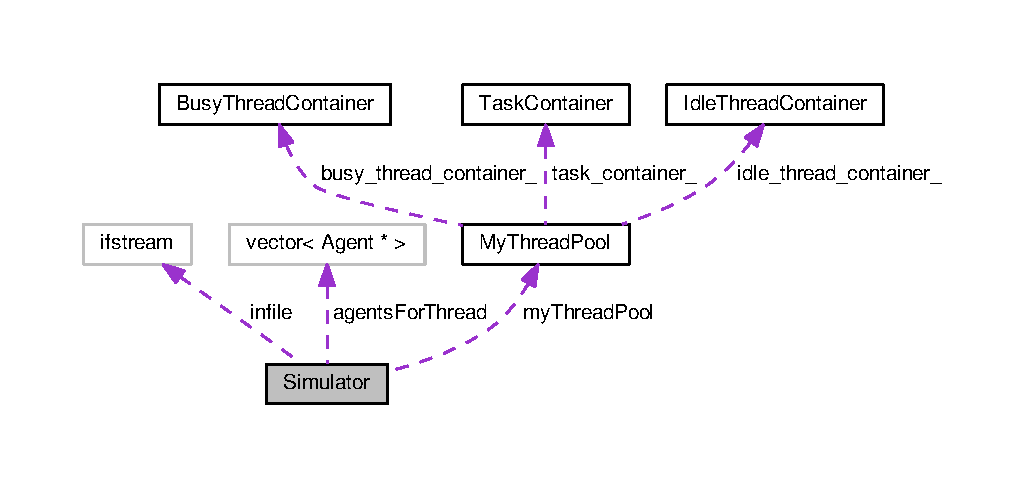
\includegraphics[width=350pt]{classSimulator__coll__graph}
\end{center}
\end{figure}
\subsection*{Public Member Functions}
\begin{DoxyCompactItemize}
\item 
\hyperlink{classSimulator_a9f689d6fe7cabbc4a31da6a3202a2428}{Simulator} (\hyperlink{main_8hpp_a4cb9f4bcd812094244f1949a88671bb8}{Simulator\+State} \&\hyperlink{classSimulator_adac2342fdb4ea403867b50df76a8d0c7}{simulator\+State}, \hyperlink{Server_8hpp_a49cc8333bde52a7f1eb36bdb3e4e8a06}{Input\+Dictionary} \&\hyperlink{classSimulator_a5d1671432b317ac4ddb63acb0267388b}{human\+Inputs}, \hyperlink{Server_8hpp_acc6d6e73aa06631da7c2f627f9979d64}{Agent\+Dictionary} \&\hyperlink{classSimulator_adc23128e4d69f004ce27410cb505bd2a}{agent\+Dictionary}, std\+::mutex \&\hyperlink{classSimulator_a7292c6375fc98bac2acd5b183aab36fb}{mutex}, \hyperlink{classMyThreadPool}{My\+Thread\+Pool} \&mythread\+Pool)
\item 
void \hyperlink{classSimulator_aa2de7e32b04cc3e8fc60aec23997621b}{run} ()
\begin{DoxyCompactList}\small\item\em Start the simulator. This is an infinite loop. \end{DoxyCompactList}\end{DoxyCompactItemize}
\subsection*{Static Public Attributes}
\begin{DoxyCompactItemize}
\item 
static \hyperlink{Server_8hpp_a49cc8333bde52a7f1eb36bdb3e4e8a06}{Input\+Dictionary} \hyperlink{classSimulator_ae91cf2cc1bc4365ea0a6072e5d2accf5}{human\+Inputs\+For\+Thread} = \hyperlink{Server_8hpp_a49cc8333bde52a7f1eb36bdb3e4e8a06}{Input\+Dictionary}()
\item 
static vector$<$ \hyperlink{classAgent}{Agent} $\ast$ $>$ \hyperlink{classSimulator_ae7447b3c665ecc437eaea013d3163b67}{agents\+For\+Thread} = vector$<$\hyperlink{classAgent}{Agent}$\ast$$>$()
\item 
static \hyperlink{Server_8hpp_acc6d6e73aa06631da7c2f627f9979d64}{Agent\+Dictionary} \hyperlink{classSimulator_a5e3d11490c6c7fec578feee96166aa44}{agent\+Dictionary\+For\+Thread}
\item 
static int \hyperlink{classSimulator_ab9f7b36020e146f22b493267fc630f82}{flag\+For\+Virtual\+Car} = 0
\item 
static int \hyperlink{classSimulator_a288aba2bf9db7bf5e05a41cbd810e6de}{manager\+For\+Virtual\+Car} = 0
\item 
static ifstream \hyperlink{classSimulator_a41ca99de68be458860955dec68b04aad}{infile}
\item 
static int \hyperlink{classSimulator_a0173a212ad88cce09b31e4d65a0e94a8}{update\+Times} = 0
\item 
static double \hyperlink{classSimulator_aa066f39b0352ed03976adf41ff67c1ab}{time} = 0.\+0
\end{DoxyCompactItemize}
\subsection*{Private Member Functions}
\begin{DoxyCompactItemize}
\item 
void \hyperlink{classSimulator_aa9bc9a3e38032f3b5e96c4466625bf5c}{update\+Tick} ()
\begin{DoxyCompactList}\small\item\em Record the agents states. Update the agents in the simulation. This is called for each iteration step. \end{DoxyCompactList}\item 
void \hyperlink{classSimulator_aad68e1807b14ca5bfd11cb7ebba25645}{reset} ()
\begin{DoxyCompactList}\small\item\em reset the simulator status \end{DoxyCompactList}\end{DoxyCompactItemize}
\subsection*{Static Private Member Functions}
\begin{DoxyCompactItemize}
\item 
static vector$<$ string $>$ \hyperlink{classSimulator_a6cd43123d84d9441152c4f416f7fe239}{split} (const string \&str, const string \&pattern)
\end{DoxyCompactItemize}
\subsection*{Private Attributes}
\begin{DoxyCompactItemize}
\item 
\hyperlink{main_8hpp_a4cb9f4bcd812094244f1949a88671bb8}{Simulator\+State} \& \hyperlink{classSimulator_adac2342fdb4ea403867b50df76a8d0c7}{simulator\+State}
\item 
\hyperlink{Server_8hpp_acc6d6e73aa06631da7c2f627f9979d64}{Agent\+Dictionary} \& \hyperlink{classSimulator_adc23128e4d69f004ce27410cb505bd2a}{agent\+Dictionary}
\item 
std\+::mutex \& \hyperlink{classSimulator_a7292c6375fc98bac2acd5b183aab36fb}{mutex}
\item 
\hyperlink{Server_8hpp_a49cc8333bde52a7f1eb36bdb3e4e8a06}{Input\+Dictionary} \& \hyperlink{classSimulator_a5d1671432b317ac4ddb63acb0267388b}{human\+Inputs}
\item 
\hyperlink{classMyThreadPool}{My\+Thread\+Pool} \& \hyperlink{classSimulator_afd96ecff25700211fcd29f3cce0c2d18}{my\+Thread\+Pool}
\item 
int \hyperlink{classSimulator_aa765c0e8bded253061bf1ffb2ba6c672}{line\+Number}
\item 
timeval \hyperlink{classSimulator_a6de4772dbd09ae8f0b9f049efada5348}{t1}
\item 
timeval \hyperlink{classSimulator_a72a269b612e7c60a7d064718a9f33f79}{t2}
\item 
double \hyperlink{classSimulator_ad243edbcd9f9b3a4fa4b6f218444f7ae}{timeuse} = 0
\end{DoxyCompactItemize}


\subsection{Detailed Description}
The class of the whole simulator. 

It manage all agents and use the thread pool to calculate the next state of each agent 

\subsection{Constructor \& Destructor Documentation}
\index{Simulator@{Simulator}!Simulator@{Simulator}}
\index{Simulator@{Simulator}!Simulator@{Simulator}}
\subsubsection[{\texorpdfstring{Simulator(\+Simulator\+State \&simulator\+State, Input\+Dictionary \&human\+Inputs, Agent\+Dictionary \&agent\+Dictionary, std\+::mutex \&mutex, My\+Thread\+Pool \&mythread\+Pool)}{Simulator(SimulatorState &simulatorState, InputDictionary &humanInputs, AgentDictionary &agentDictionary, std::mutex &mutex, MyThreadPool &mythreadPool)}}]{\setlength{\rightskip}{0pt plus 5cm}Simulator\+::\+Simulator (
\begin{DoxyParamCaption}
\item[{{\bf Simulator\+State} \&}]{simulator\+State, }
\item[{{\bf Input\+Dictionary} \&}]{human\+Inputs, }
\item[{{\bf Agent\+Dictionary} \&}]{agent\+Dictionary, }
\item[{std\+::mutex \&}]{mutex, }
\item[{{\bf My\+Thread\+Pool} \&}]{my\+Thread\+Pool}
\end{DoxyParamCaption}
)}\hypertarget{classSimulator_a9f689d6fe7cabbc4a31da6a3202a2428}{}\label{classSimulator_a9f689d6fe7cabbc4a31da6a3202a2428}

\begin{DoxyParams}{Parameters}
{\em simulator\+State} & reference to the simulator state, an enumerator. \\
\hline
{\em human\+Inputs} & reference to a map from agent to pertaining vector human input. \\
\hline
{\em agent\+Dictionary} & reference to a map from agent to pertaining controller, model, and planner. \\
\hline
{\em mutex} & reference to a global mutex lock, which avoids thread conflicts. \\
\hline
\end{DoxyParams}


\subsection{Member Function Documentation}
\index{Simulator@{Simulator}!reset@{reset}}
\index{reset@{reset}!Simulator@{Simulator}}
\subsubsection[{\texorpdfstring{reset()}{reset()}}]{\setlength{\rightskip}{0pt plus 5cm}void Simulator\+::reset (
\begin{DoxyParamCaption}
{}
\end{DoxyParamCaption}
)\hspace{0.3cm}{\ttfamily [private]}}\hypertarget{classSimulator_aad68e1807b14ca5bfd11cb7ebba25645}{}\label{classSimulator_aad68e1807b14ca5bfd11cb7ebba25645}


reset the simulator status 

\index{Simulator@{Simulator}!run@{run}}
\index{run@{run}!Simulator@{Simulator}}
\subsubsection[{\texorpdfstring{run()}{run()}}]{\setlength{\rightskip}{0pt plus 5cm}void Simulator\+::run (
\begin{DoxyParamCaption}
{}
\end{DoxyParamCaption}
)}\hypertarget{classSimulator_aa2de7e32b04cc3e8fc60aec23997621b}{}\label{classSimulator_aa2de7e32b04cc3e8fc60aec23997621b}


Start the simulator. This is an infinite loop. 

\index{Simulator@{Simulator}!split@{split}}
\index{split@{split}!Simulator@{Simulator}}
\subsubsection[{\texorpdfstring{split(const string \&str, const string \&pattern)}{split(const string &str, const string &pattern)}}]{\setlength{\rightskip}{0pt plus 5cm}static vector$<$string$>$ Simulator\+::split (
\begin{DoxyParamCaption}
\item[{const string \&}]{str, }
\item[{const string \&}]{pattern}
\end{DoxyParamCaption}
)\hspace{0.3cm}{\ttfamily [inline]}, {\ttfamily [static]}, {\ttfamily [private]}}\hypertarget{classSimulator_a6cd43123d84d9441152c4f416f7fe239}{}\label{classSimulator_a6cd43123d84d9441152c4f416f7fe239}
\index{Simulator@{Simulator}!update\+Tick@{update\+Tick}}
\index{update\+Tick@{update\+Tick}!Simulator@{Simulator}}
\subsubsection[{\texorpdfstring{update\+Tick()}{updateTick()}}]{\setlength{\rightskip}{0pt plus 5cm}void Simulator\+::update\+Tick (
\begin{DoxyParamCaption}
{}
\end{DoxyParamCaption}
)\hspace{0.3cm}{\ttfamily [private]}}\hypertarget{classSimulator_aa9bc9a3e38032f3b5e96c4466625bf5c}{}\label{classSimulator_aa9bc9a3e38032f3b5e96c4466625bf5c}


Record the agents states. Update the agents in the simulation. This is called for each iteration step. 



\subsection{Member Data Documentation}
\index{Simulator@{Simulator}!agent\+Dictionary@{agent\+Dictionary}}
\index{agent\+Dictionary@{agent\+Dictionary}!Simulator@{Simulator}}
\subsubsection[{\texorpdfstring{agent\+Dictionary}{agentDictionary}}]{\setlength{\rightskip}{0pt plus 5cm}{\bf Agent\+Dictionary}\& Simulator\+::agent\+Dictionary\hspace{0.3cm}{\ttfamily [private]}}\hypertarget{classSimulator_adc23128e4d69f004ce27410cb505bd2a}{}\label{classSimulator_adc23128e4d69f004ce27410cb505bd2a}
Reference to a map from agent to pertaining controller, model, and planner. \index{Simulator@{Simulator}!agent\+Dictionary\+For\+Thread@{agent\+Dictionary\+For\+Thread}}
\index{agent\+Dictionary\+For\+Thread@{agent\+Dictionary\+For\+Thread}!Simulator@{Simulator}}
\subsubsection[{\texorpdfstring{agent\+Dictionary\+For\+Thread}{agentDictionaryForThread}}]{\setlength{\rightskip}{0pt plus 5cm}{\bf Agent\+Dictionary} Simulator\+::agent\+Dictionary\+For\+Thread\hspace{0.3cm}{\ttfamily [static]}}\hypertarget{classSimulator_a5e3d11490c6c7fec578feee96166aa44}{}\label{classSimulator_a5e3d11490c6c7fec578feee96166aa44}
\index{Simulator@{Simulator}!agents\+For\+Thread@{agents\+For\+Thread}}
\index{agents\+For\+Thread@{agents\+For\+Thread}!Simulator@{Simulator}}
\subsubsection[{\texorpdfstring{agents\+For\+Thread}{agentsForThread}}]{\setlength{\rightskip}{0pt plus 5cm}vector$<$ {\bf Agent} $\ast$ $>$ Simulator\+::agents\+For\+Thread = vector$<${\bf Agent}$\ast$$>$()\hspace{0.3cm}{\ttfamily [static]}}\hypertarget{classSimulator_ae7447b3c665ecc437eaea013d3163b67}{}\label{classSimulator_ae7447b3c665ecc437eaea013d3163b67}
Reference to a vector for all agents\textquotesingle{} information that should be used for calculate this time. \index{Simulator@{Simulator}!flag\+For\+Virtual\+Car@{flag\+For\+Virtual\+Car}}
\index{flag\+For\+Virtual\+Car@{flag\+For\+Virtual\+Car}!Simulator@{Simulator}}
\subsubsection[{\texorpdfstring{flag\+For\+Virtual\+Car}{flagForVirtualCar}}]{\setlength{\rightskip}{0pt plus 5cm}int Simulator\+::flag\+For\+Virtual\+Car = 0\hspace{0.3cm}{\ttfamily [static]}}\hypertarget{classSimulator_ab9f7b36020e146f22b493267fc630f82}{}\label{classSimulator_ab9f7b36020e146f22b493267fc630f82}
Decide whether update virtual car, based on timeuse $>$ 0.\+01?. \index{Simulator@{Simulator}!human\+Inputs@{human\+Inputs}}
\index{human\+Inputs@{human\+Inputs}!Simulator@{Simulator}}
\subsubsection[{\texorpdfstring{human\+Inputs}{humanInputs}}]{\setlength{\rightskip}{0pt plus 5cm}{\bf Input\+Dictionary}\& Simulator\+::human\+Inputs\hspace{0.3cm}{\ttfamily [private]}}\hypertarget{classSimulator_a5d1671432b317ac4ddb63acb0267388b}{}\label{classSimulator_a5d1671432b317ac4ddb63acb0267388b}
Reference to a map from agent to pertaining vector human input. \index{Simulator@{Simulator}!human\+Inputs\+For\+Thread@{human\+Inputs\+For\+Thread}}
\index{human\+Inputs\+For\+Thread@{human\+Inputs\+For\+Thread}!Simulator@{Simulator}}
\subsubsection[{\texorpdfstring{human\+Inputs\+For\+Thread}{humanInputsForThread}}]{\setlength{\rightskip}{0pt plus 5cm}{\bf Input\+Dictionary} Simulator\+::human\+Inputs\+For\+Thread = {\bf Input\+Dictionary}()\hspace{0.3cm}{\ttfamily [static]}}\hypertarget{classSimulator_ae91cf2cc1bc4365ea0a6072e5d2accf5}{}\label{classSimulator_ae91cf2cc1bc4365ea0a6072e5d2accf5}
Reference to a map from agent to pertaining vector human input that should be used for calculate this time. \index{Simulator@{Simulator}!infile@{infile}}
\index{infile@{infile}!Simulator@{Simulator}}
\subsubsection[{\texorpdfstring{infile}{infile}}]{\setlength{\rightskip}{0pt plus 5cm}ifstream Simulator\+::infile\hspace{0.3cm}{\ttfamily [static]}}\hypertarget{classSimulator_a41ca99de68be458860955dec68b04aad}{}\label{classSimulator_a41ca99de68be458860955dec68b04aad}
.txt file for record all agents states. \index{Simulator@{Simulator}!line\+Number@{line\+Number}}
\index{line\+Number@{line\+Number}!Simulator@{Simulator}}
\subsubsection[{\texorpdfstring{line\+Number}{lineNumber}}]{\setlength{\rightskip}{0pt plus 5cm}int Simulator\+::line\+Number\hspace{0.3cm}{\ttfamily [private]}}\hypertarget{classSimulator_aa765c0e8bded253061bf1ffb2ba6c672}{}\label{classSimulator_aa765c0e8bded253061bf1ffb2ba6c672}
\index{Simulator@{Simulator}!manager\+For\+Virtual\+Car@{manager\+For\+Virtual\+Car}}
\index{manager\+For\+Virtual\+Car@{manager\+For\+Virtual\+Car}!Simulator@{Simulator}}
\subsubsection[{\texorpdfstring{manager\+For\+Virtual\+Car}{managerForVirtualCar}}]{\setlength{\rightskip}{0pt plus 5cm}int Simulator\+::manager\+For\+Virtual\+Car = 0\hspace{0.3cm}{\ttfamily [static]}}\hypertarget{classSimulator_a288aba2bf9db7bf5e05a41cbd810e6de}{}\label{classSimulator_a288aba2bf9db7bf5e05a41cbd810e6de}
Decide whether begin to add the virtual car. \index{Simulator@{Simulator}!mutex@{mutex}}
\index{mutex@{mutex}!Simulator@{Simulator}}
\subsubsection[{\texorpdfstring{mutex}{mutex}}]{\setlength{\rightskip}{0pt plus 5cm}std\+::mutex\& Simulator\+::mutex\hspace{0.3cm}{\ttfamily [private]}}\hypertarget{classSimulator_a7292c6375fc98bac2acd5b183aab36fb}{}\label{classSimulator_a7292c6375fc98bac2acd5b183aab36fb}
Reference to a global mutex lock, which avoids thread conflicts. \index{Simulator@{Simulator}!my\+Thread\+Pool@{my\+Thread\+Pool}}
\index{my\+Thread\+Pool@{my\+Thread\+Pool}!Simulator@{Simulator}}
\subsubsection[{\texorpdfstring{my\+Thread\+Pool}{myThreadPool}}]{\setlength{\rightskip}{0pt plus 5cm}{\bf My\+Thread\+Pool}\& Simulator\+::my\+Thread\+Pool\hspace{0.3cm}{\ttfamily [private]}}\hypertarget{classSimulator_afd96ecff25700211fcd29f3cce0c2d18}{}\label{classSimulator_afd96ecff25700211fcd29f3cce0c2d18}
The thread pool for calculate all agents \index{Simulator@{Simulator}!simulator\+State@{simulator\+State}}
\index{simulator\+State@{simulator\+State}!Simulator@{Simulator}}
\subsubsection[{\texorpdfstring{simulator\+State}{simulatorState}}]{\setlength{\rightskip}{0pt plus 5cm}{\bf Simulator\+State}\& Simulator\+::simulator\+State\hspace{0.3cm}{\ttfamily [private]}}\hypertarget{classSimulator_adac2342fdb4ea403867b50df76a8d0c7}{}\label{classSimulator_adac2342fdb4ea403867b50df76a8d0c7}
Reference to the simulator state, an enumerator. \index{Simulator@{Simulator}!t1@{t1}}
\index{t1@{t1}!Simulator@{Simulator}}
\subsubsection[{\texorpdfstring{t1}{t1}}]{\setlength{\rightskip}{0pt plus 5cm}timeval Simulator\+::t1\hspace{0.3cm}{\ttfamily [private]}}\hypertarget{classSimulator_a6de4772dbd09ae8f0b9f049efada5348}{}\label{classSimulator_a6de4772dbd09ae8f0b9f049efada5348}
\index{Simulator@{Simulator}!t2@{t2}}
\index{t2@{t2}!Simulator@{Simulator}}
\subsubsection[{\texorpdfstring{t2}{t2}}]{\setlength{\rightskip}{0pt plus 5cm}timeval Simulator\+::t2\hspace{0.3cm}{\ttfamily [private]}}\hypertarget{classSimulator_a72a269b612e7c60a7d064718a9f33f79}{}\label{classSimulator_a72a269b612e7c60a7d064718a9f33f79}
Timeval for getting time used for arrange task for all agents \index{Simulator@{Simulator}!time@{time}}
\index{time@{time}!Simulator@{Simulator}}
\subsubsection[{\texorpdfstring{time}{time}}]{\setlength{\rightskip}{0pt plus 5cm}double Simulator\+::time = 0.\+0\hspace{0.3cm}{\ttfamily [static]}}\hypertarget{classSimulator_aa066f39b0352ed03976adf41ff67c1ab}{}\label{classSimulator_aa066f39b0352ed03976adf41ff67c1ab}
Record the time that the simulator cost for last updating, which is used to get timeuse. \index{Simulator@{Simulator}!timeuse@{timeuse}}
\index{timeuse@{timeuse}!Simulator@{Simulator}}
\subsubsection[{\texorpdfstring{timeuse}{timeuse}}]{\setlength{\rightskip}{0pt plus 5cm}double Simulator\+::timeuse = 0\hspace{0.3cm}{\ttfamily [private]}}\hypertarget{classSimulator_ad243edbcd9f9b3a4fa4b6f218444f7ae}{}\label{classSimulator_ad243edbcd9f9b3a4fa4b6f218444f7ae}
Record the time used and reset to 0 when it over 0.\+01 \index{Simulator@{Simulator}!update\+Times@{update\+Times}}
\index{update\+Times@{update\+Times}!Simulator@{Simulator}}
\subsubsection[{\texorpdfstring{update\+Times}{updateTimes}}]{\setlength{\rightskip}{0pt plus 5cm}int Simulator\+::update\+Times = 0\hspace{0.3cm}{\ttfamily [static]}}\hypertarget{classSimulator_a0173a212ad88cce09b31e4d65a0e94a8}{}\label{classSimulator_a0173a212ad88cce09b31e4d65a0e94a8}
Counter for how many times the simulator have updated 

The documentation for this class was generated from the following files\+:\begin{DoxyCompactItemize}
\item 
Simulator/\hyperlink{Simulator_8hpp}{Simulator.\+hpp}\item 
Simulator/\hyperlink{Simulator_8cpp}{Simulator.\+cpp}\end{DoxyCompactItemize}

\hypertarget{classTask}{}\section{Task Class Reference}
\label{classTask}\index{Task@{Task}}


The class of task.  




{\ttfamily \#include $<$Task.\+hpp$>$}



Inheritance diagram for Task\+:\nopagebreak
\begin{figure}[H]
\begin{center}
\leavevmode
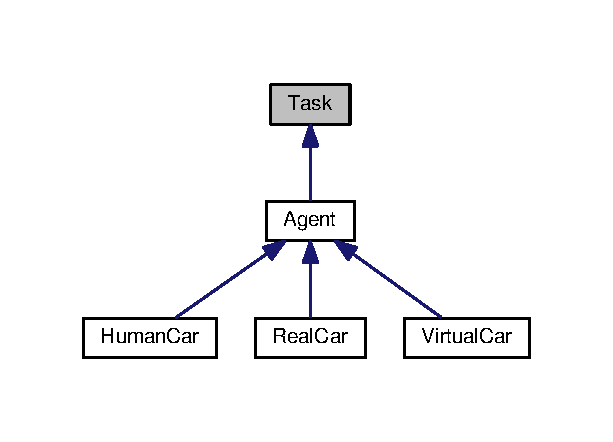
\includegraphics[width=294pt]{classTask__inherit__graph}
\end{center}
\end{figure}
\subsection*{Public Member Functions}
\begin{DoxyCompactItemize}
\item 
\hyperlink{classTask_a0ca53354bdc006762a0fda68c64f7608}{Task} ()
\item 
void \hyperlink{classTask_abf2fe0d1d748f8efee8fdf86f588ebcb}{Set\+Priority} (int priority)
\begin{DoxyCompactList}\small\item\em set priority. \end{DoxyCompactList}\item 
virtual void \hyperlink{classTask_a18ea998d77c751e6e1581f7035022a5b}{Run} ()
\end{DoxyCompactItemize}
\subsection*{Protected Attributes}
\begin{DoxyCompactItemize}
\item 
int \hyperlink{classTask_ad7d1b58e73a2d716dabd08ab985a35f9}{priority\+\_\+}
\end{DoxyCompactItemize}


\subsection{Detailed Description}
The class of task. 

\subsection{Constructor \& Destructor Documentation}
\index{Task@{Task}!Task@{Task}}
\index{Task@{Task}!Task@{Task}}
\subsubsection[{\texorpdfstring{Task()}{Task()}}]{\setlength{\rightskip}{0pt plus 5cm}Task\+::\+Task (
\begin{DoxyParamCaption}
{}
\end{DoxyParamCaption}
)\hspace{0.3cm}{\ttfamily [inline]}}\hypertarget{classTask_a0ca53354bdc006762a0fda68c64f7608}{}\label{classTask_a0ca53354bdc006762a0fda68c64f7608}


\subsection{Member Function Documentation}
\index{Task@{Task}!Run@{Run}}
\index{Run@{Run}!Task@{Task}}
\subsubsection[{\texorpdfstring{Run()}{Run()}}]{\setlength{\rightskip}{0pt plus 5cm}void Task\+::\+Run (
\begin{DoxyParamCaption}
{}
\end{DoxyParamCaption}
)\hspace{0.3cm}{\ttfamily [virtual]}}\hypertarget{classTask_a18ea998d77c751e6e1581f7035022a5b}{}\label{classTask_a18ea998d77c751e6e1581f7035022a5b}


Reimplemented in \hyperlink{classAgent_a80e144d0fd78f8e1a54abf92158448e1}{Agent}.

\index{Task@{Task}!Set\+Priority@{Set\+Priority}}
\index{Set\+Priority@{Set\+Priority}!Task@{Task}}
\subsubsection[{\texorpdfstring{Set\+Priority(int priority)}{SetPriority(int priority)}}]{\setlength{\rightskip}{0pt plus 5cm}void Task\+::\+Set\+Priority (
\begin{DoxyParamCaption}
\item[{int}]{priority}
\end{DoxyParamCaption}
)\hspace{0.3cm}{\ttfamily [inline]}}\hypertarget{classTask_abf2fe0d1d748f8efee8fdf86f588ebcb}{}\label{classTask_abf2fe0d1d748f8efee8fdf86f588ebcb}


set priority. 



\subsection{Member Data Documentation}
\index{Task@{Task}!priority\+\_\+@{priority\+\_\+}}
\index{priority\+\_\+@{priority\+\_\+}!Task@{Task}}
\subsubsection[{\texorpdfstring{priority\+\_\+}{priority_}}]{\setlength{\rightskip}{0pt plus 5cm}int Task\+::priority\+\_\+\hspace{0.3cm}{\ttfamily [protected]}}\hypertarget{classTask_ad7d1b58e73a2d716dabd08ab985a35f9}{}\label{classTask_ad7d1b58e73a2d716dabd08ab985a35f9}
The priority of this task. The range of weight is 1 to 50. 

The documentation for this class was generated from the following files\+:\begin{DoxyCompactItemize}
\item 
thread\+Pool/\hyperlink{Task_8hpp}{Task.\+hpp}\item 
thread\+Pool/\hyperlink{Task_8cpp}{Task.\+cpp}\end{DoxyCompactItemize}

\hypertarget{classTaskContainer}{}\section{Task\+Container Class Reference}
\label{classTaskContainer}\index{Task\+Container@{Task\+Container}}


The class of task container.  




{\ttfamily \#include $<$Task\+Container.\+hpp$>$}

\subsection*{Public Member Functions}
\begin{DoxyCompactItemize}
\item 
\hyperlink{classTaskContainer_a7e3135258232a3fad842ce5006fe30b0}{Task\+Container} ()
\item 
\hyperlink{classTaskContainer_a8d7a3ea804743f8d263399134e82a27b}{$\sim$\+Task\+Container} ()
\item 
void \hyperlink{classTaskContainer_afa83fd5f9b758c356cdb7838f953ec1d}{push} (\hyperlink{classTask}{Task} $\ast$)
\begin{DoxyCompactList}\small\item\em Push a task into the task container. \end{DoxyCompactList}\item 
\hyperlink{classTask}{Task} $\ast$ \hyperlink{classTaskContainer_a32bb364b0b32e907fceeb9a2fb49d2f3}{top} ()
\begin{DoxyCompactList}\small\item\em Get the top task from the task container. \end{DoxyCompactList}\item 
void \hyperlink{classTaskContainer_ae50a94fbdf60d08bf66e586ba5b94ad0}{pop} ()
\begin{DoxyCompactList}\small\item\em Get the top task from the task container. \end{DoxyCompactList}\item 
std\+::priority\+\_\+queue$<$ \hyperlink{classTask}{Task} $\ast$ $>$\+::size\+\_\+type \hyperlink{classTaskContainer_ad195d3caf63e1deea6244973b603ce63}{size} ()
\begin{DoxyCompactList}\small\item\em Get the number of tasks in the task container. \end{DoxyCompactList}\end{DoxyCompactItemize}
\subsection*{Private Attributes}
\begin{DoxyCompactItemize}
\item 
std\+::priority\+\_\+queue$<$ \hyperlink{classTask}{Task} $\ast$ $>$ \hyperlink{classTaskContainer_a289e207c3a66e721fa6930480322907e}{task\+\_\+container\+\_\+}
\end{DoxyCompactItemize}


\subsection{Detailed Description}
The class of task container. 

It contains task that need to be assigned. 

\subsection{Constructor \& Destructor Documentation}
\index{Task\+Container@{Task\+Container}!Task\+Container@{Task\+Container}}
\index{Task\+Container@{Task\+Container}!Task\+Container@{Task\+Container}}
\subsubsection[{\texorpdfstring{Task\+Container()}{TaskContainer()}}]{\setlength{\rightskip}{0pt plus 5cm}Task\+Container\+::\+Task\+Container (
\begin{DoxyParamCaption}
{}
\end{DoxyParamCaption}
)}\hypertarget{classTaskContainer_a7e3135258232a3fad842ce5006fe30b0}{}\label{classTaskContainer_a7e3135258232a3fad842ce5006fe30b0}
\index{Task\+Container@{Task\+Container}!````~Task\+Container@{$\sim$\+Task\+Container}}
\index{````~Task\+Container@{$\sim$\+Task\+Container}!Task\+Container@{Task\+Container}}
\subsubsection[{\texorpdfstring{$\sim$\+Task\+Container()}{~TaskContainer()}}]{\setlength{\rightskip}{0pt plus 5cm}Task\+Container\+::$\sim$\+Task\+Container (
\begin{DoxyParamCaption}
{}
\end{DoxyParamCaption}
)}\hypertarget{classTaskContainer_a8d7a3ea804743f8d263399134e82a27b}{}\label{classTaskContainer_a8d7a3ea804743f8d263399134e82a27b}


\subsection{Member Function Documentation}
\index{Task\+Container@{Task\+Container}!pop@{pop}}
\index{pop@{pop}!Task\+Container@{Task\+Container}}
\subsubsection[{\texorpdfstring{pop()}{pop()}}]{\setlength{\rightskip}{0pt plus 5cm}void Task\+Container\+::pop (
\begin{DoxyParamCaption}
{}
\end{DoxyParamCaption}
)}\hypertarget{classTaskContainer_ae50a94fbdf60d08bf66e586ba5b94ad0}{}\label{classTaskContainer_ae50a94fbdf60d08bf66e586ba5b94ad0}


Get the top task from the task container. 

\index{Task\+Container@{Task\+Container}!push@{push}}
\index{push@{push}!Task\+Container@{Task\+Container}}
\subsubsection[{\texorpdfstring{push(\+Task $\ast$)}{push(Task *)}}]{\setlength{\rightskip}{0pt plus 5cm}void Task\+Container\+::push (
\begin{DoxyParamCaption}
\item[{{\bf Task} $\ast$}]{t}
\end{DoxyParamCaption}
)}\hypertarget{classTaskContainer_afa83fd5f9b758c356cdb7838f953ec1d}{}\label{classTaskContainer_afa83fd5f9b758c356cdb7838f953ec1d}


Push a task into the task container. 

\index{Task\+Container@{Task\+Container}!size@{size}}
\index{size@{size}!Task\+Container@{Task\+Container}}
\subsubsection[{\texorpdfstring{size()}{size()}}]{\setlength{\rightskip}{0pt plus 5cm}std\+::priority\+\_\+queue$<$ {\bf Task} $\ast$ $>$\+::size\+\_\+type Task\+Container\+::size (
\begin{DoxyParamCaption}
{}
\end{DoxyParamCaption}
)}\hypertarget{classTaskContainer_ad195d3caf63e1deea6244973b603ce63}{}\label{classTaskContainer_ad195d3caf63e1deea6244973b603ce63}


Get the number of tasks in the task container. 

\index{Task\+Container@{Task\+Container}!top@{top}}
\index{top@{top}!Task\+Container@{Task\+Container}}
\subsubsection[{\texorpdfstring{top()}{top()}}]{\setlength{\rightskip}{0pt plus 5cm}{\bf Task} $\ast$ Task\+Container\+::top (
\begin{DoxyParamCaption}
{}
\end{DoxyParamCaption}
)}\hypertarget{classTaskContainer_a32bb364b0b32e907fceeb9a2fb49d2f3}{}\label{classTaskContainer_a32bb364b0b32e907fceeb9a2fb49d2f3}


Get the top task from the task container. 



\subsection{Member Data Documentation}
\index{Task\+Container@{Task\+Container}!task\+\_\+container\+\_\+@{task\+\_\+container\+\_\+}}
\index{task\+\_\+container\+\_\+@{task\+\_\+container\+\_\+}!Task\+Container@{Task\+Container}}
\subsubsection[{\texorpdfstring{task\+\_\+container\+\_\+}{task_container_}}]{\setlength{\rightskip}{0pt plus 5cm}std\+::priority\+\_\+queue$<${\bf Task}$\ast$$>$ Task\+Container\+::task\+\_\+container\+\_\+\hspace{0.3cm}{\ttfamily [private]}}\hypertarget{classTaskContainer_a289e207c3a66e721fa6930480322907e}{}\label{classTaskContainer_a289e207c3a66e721fa6930480322907e}
The task container itself 

The documentation for this class was generated from the following files\+:\begin{DoxyCompactItemize}
\item 
thread\+Pool/\hyperlink{TaskContainer_8hpp}{Task\+Container.\+hpp}\item 
thread\+Pool/\hyperlink{TaskContainer_8cpp}{Task\+Container.\+cpp}\end{DoxyCompactItemize}

\hypertarget{classTrivialPlanner}{}\section{Trivial\+Planner Class Reference}
\label{classTrivialPlanner}\index{Trivial\+Planner@{Trivial\+Planner}}


\hyperlink{classPlanner}{Planner} for the real car.  




{\ttfamily \#include $<$Trivial\+Planner.\+hpp$>$}



Inheritance diagram for Trivial\+Planner\+:\nopagebreak
\begin{figure}[H]
\begin{center}
\leavevmode
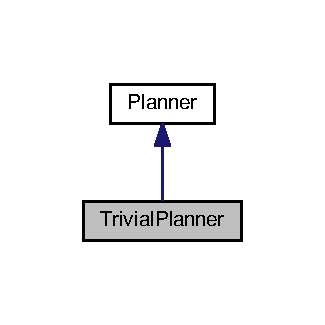
\includegraphics[width=156pt]{classTrivialPlanner__inherit__graph}
\end{center}
\end{figure}


Collaboration diagram for Trivial\+Planner\+:\nopagebreak
\begin{figure}[H]
\begin{center}
\leavevmode
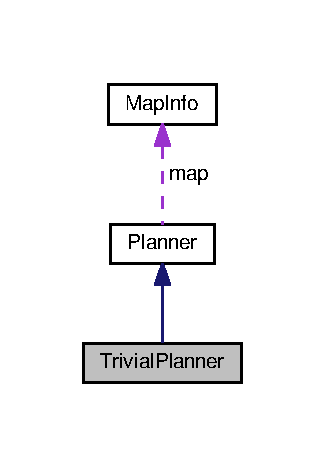
\includegraphics[width=156pt]{classTrivialPlanner__coll__graph}
\end{center}
\end{figure}
\subsection*{Public Member Functions}
\begin{DoxyCompactItemize}
\item 
\hyperlink{classTrivialPlanner_a52d2aa905883a1a9a80181151e781405}{Trivial\+Planner} ()
\item 
\hyperlink{Agent_8hpp_a5dd127bb3cb18b011cf5fd80a906e830}{Vector} \hyperlink{classTrivialPlanner_a27317c7986fd79906da5964dd893c5e9}{update} (\hyperlink{Agent_8hpp_a5dd127bb3cb18b011cf5fd80a906e830}{Vector} current\+State, const \hyperlink{Agent_8hpp_a5dd127bb3cb18b011cf5fd80a906e830}{Vector} \&human\+Input, std\+::vector$<$ \hyperlink{classAgent}{Agent} $\ast$ $>$ agents) override
\end{DoxyCompactItemize}
\subsection*{Additional Inherited Members}


\subsection{Detailed Description}
\hyperlink{classPlanner}{Planner} for the real car. 

\subsection{Constructor \& Destructor Documentation}
\index{Trivial\+Planner@{Trivial\+Planner}!Trivial\+Planner@{Trivial\+Planner}}
\index{Trivial\+Planner@{Trivial\+Planner}!Trivial\+Planner@{Trivial\+Planner}}
\subsubsection[{\texorpdfstring{Trivial\+Planner()}{TrivialPlanner()}}]{\setlength{\rightskip}{0pt plus 5cm}Trivial\+Planner\+::\+Trivial\+Planner (
\begin{DoxyParamCaption}
{}
\end{DoxyParamCaption}
)\hspace{0.3cm}{\ttfamily [explicit]}}\hypertarget{classTrivialPlanner_a52d2aa905883a1a9a80181151e781405}{}\label{classTrivialPlanner_a52d2aa905883a1a9a80181151e781405}
Constructor. Dimension of state vector is 6 (x, y, yaw, speed x, speed y, speed yaw) Dimension of input vector is 6 + 4 $\ast$ P\+L\+A\+N\+\_\+\+S\+T\+EP (current state and P\+L\+A\+N\+\_\+\+S\+T\+EP state(t, x , y, v) that want to follow) 

\subsection{Member Function Documentation}
\index{Trivial\+Planner@{Trivial\+Planner}!update@{update}}
\index{update@{update}!Trivial\+Planner@{Trivial\+Planner}}
\subsubsection[{\texorpdfstring{update(\+Vector current\+State, const Vector \&human\+Input, std\+::vector$<$ Agent $\ast$ $>$ agents) override}{update(Vector currentState, const Vector &humanInput, std::vector< Agent * > agents) override}}]{\setlength{\rightskip}{0pt plus 5cm}{\bf Vector} Trivial\+Planner\+::update (
\begin{DoxyParamCaption}
\item[{{\bf Vector}}]{current\+State, }
\item[{const {\bf Vector} \&}]{human\+Input, }
\item[{std\+::vector$<$ {\bf Agent} $\ast$ $>$}]{agents}
\end{DoxyParamCaption}
)\hspace{0.3cm}{\ttfamily [override]}, {\ttfamily [virtual]}}\hypertarget{classTrivialPlanner_a27317c7986fd79906da5964dd893c5e9}{}\label{classTrivialPlanner_a27317c7986fd79906da5964dd893c5e9}
For now, it just get planned x, y and v via current state (assuming const v). 
\begin{DoxyParams}{Parameters}
{\em current\+State} & current state of the car. \\
\hline
{\em human\+Input} & current human input vector (gas pedal, brake pedal, and steering angle). doesn\textquotesingle{}t be used. \\
\hline
{\em agents} & information of all agents in the simulator. Doesn\textquotesingle{}t be used \\
\hline
\end{DoxyParams}
\begin{DoxyReturn}{Returns}
current state and P\+L\+A\+N\+\_\+\+S\+T\+EP state(t, x , y, v) that want to follow. 
\end{DoxyReturn}


Implements \hyperlink{classPlanner_a62e1434402a3f36b0883e069a10447d8}{Planner}.



The documentation for this class was generated from the following files\+:\begin{DoxyCompactItemize}
\item 
Planners/\hyperlink{TrivialPlanner_8hpp}{Trivial\+Planner.\+hpp}\item 
Planners/\hyperlink{TrivialPlanner_8cpp}{Trivial\+Planner.\+cpp}\end{DoxyCompactItemize}

\hypertarget{classVirtualCar}{}\section{Virtual\+Car Class Reference}
\label{classVirtualCar}\index{Virtual\+Car@{Virtual\+Car}}


{\ttfamily \#include $<$Virtual\+Car.\+hpp$>$}



Inheritance diagram for Virtual\+Car\+:\nopagebreak
\begin{figure}[H]
\begin{center}
\leavevmode
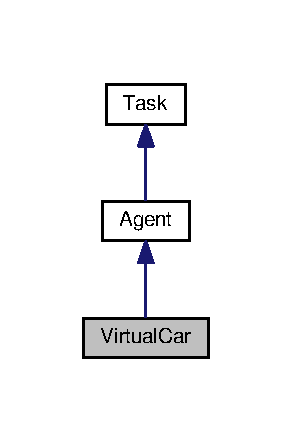
\includegraphics[width=140pt]{classVirtualCar__inherit__graph}
\end{center}
\end{figure}


Collaboration diagram for Virtual\+Car\+:\nopagebreak
\begin{figure}[H]
\begin{center}
\leavevmode
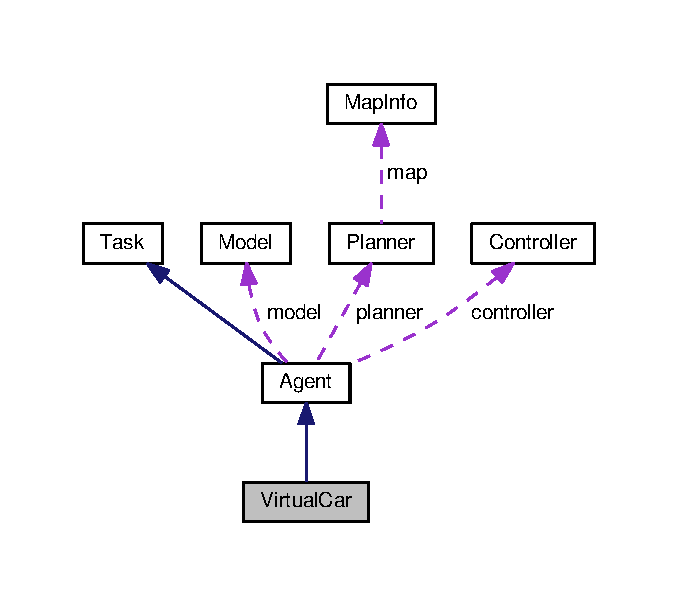
\includegraphics[width=326pt]{classVirtualCar__coll__graph}
\end{center}
\end{figure}
\subsection*{Public Member Functions}
\begin{DoxyCompactItemize}
\item 
\hyperlink{classVirtualCar_acdb26a4e0236053103eb89fe84069779}{Virtual\+Car} (int \hyperlink{classAgent_af8b58fe9dafe460ed2ddf87435a7feed}{id}, \hyperlink{Agent_8hpp_a5dd127bb3cb18b011cf5fd80a906e830}{Vector} initial\+State)
\item 
\hyperlink{classVirtualCar_a8eb1f764d7ed9a701e15b304ce9b3d4c}{Virtual\+Car} (int \hyperlink{classAgent_af8b58fe9dafe460ed2ddf87435a7feed}{id}, \hyperlink{Agent_8hpp_a5dd127bb3cb18b011cf5fd80a906e830}{Vector} initial\+State, \hyperlink{classPlanner}{Planner} $\ast$\hyperlink{classAgent_aa71be9f465a3d8eed4e3297d8aa49eb1}{planner}, \hyperlink{classController}{Controller} $\ast$\hyperlink{classAgent_a35138f4fa7fa31760928b84680f7a886}{controller}, \hyperlink{classModel}{Model} $\ast$\hyperlink{classAgent_a41c7b65f7ad35cc6756cf0313edaa9a0}{model})
\item 
\hyperlink{Agent_8hpp_ad2c3439c0fbb853c45129639d2581c51}{Agent\+Type} \hyperlink{classVirtualCar_a642228555a81aef7d410b162b0437cf2}{get\+Type} () const override
\end{DoxyCompactItemize}
\subsection*{Additional Inherited Members}


\subsection{Detailed Description}
\hyperlink{classVirtualCar}{Virtual\+Car} is a kind of agent that is not exist in the real world. Its state maybe comes from a .txt file or calculating. 

\subsection{Constructor \& Destructor Documentation}
\index{Virtual\+Car@{Virtual\+Car}!Virtual\+Car@{Virtual\+Car}}
\index{Virtual\+Car@{Virtual\+Car}!Virtual\+Car@{Virtual\+Car}}
\subsubsection[{\texorpdfstring{Virtual\+Car(int id, Vector initial\+State)}{VirtualCar(int id, Vector initialState)}}]{\setlength{\rightskip}{0pt plus 5cm}Virtual\+Car\+::\+Virtual\+Car (
\begin{DoxyParamCaption}
\item[{int}]{id, }
\item[{{\bf Vector}}]{initial\+State}
\end{DoxyParamCaption}
)}\hypertarget{classVirtualCar_acdb26a4e0236053103eb89fe84069779}{}\label{classVirtualCar_acdb26a4e0236053103eb89fe84069779}
\index{Virtual\+Car@{Virtual\+Car}!Virtual\+Car@{Virtual\+Car}}
\index{Virtual\+Car@{Virtual\+Car}!Virtual\+Car@{Virtual\+Car}}
\subsubsection[{\texorpdfstring{Virtual\+Car(int id, Vector initial\+State, Planner $\ast$planner, Controller $\ast$controller, Model $\ast$model)}{VirtualCar(int id, Vector initialState, Planner *planner, Controller *controller, Model *model)}}]{\setlength{\rightskip}{0pt plus 5cm}Virtual\+Car\+::\+Virtual\+Car (
\begin{DoxyParamCaption}
\item[{int}]{id, }
\item[{{\bf Vector}}]{initial\+State, }
\item[{{\bf Planner} $\ast$}]{planner, }
\item[{{\bf Controller} $\ast$}]{controller, }
\item[{{\bf Model} $\ast$}]{model}
\end{DoxyParamCaption}
)\hspace{0.3cm}{\ttfamily [explicit]}}\hypertarget{classVirtualCar_a8eb1f764d7ed9a701e15b304ce9b3d4c}{}\label{classVirtualCar_a8eb1f764d7ed9a701e15b304ce9b3d4c}
Constructor. 
\begin{DoxyParams}{Parameters}
{\em id} & id of the new virtual car. \\
\hline
{\em initial\+State} & initial state of the virtual car. \\
\hline
\end{DoxyParams}


\subsection{Member Function Documentation}
\index{Virtual\+Car@{Virtual\+Car}!get\+Type@{get\+Type}}
\index{get\+Type@{get\+Type}!Virtual\+Car@{Virtual\+Car}}
\subsubsection[{\texorpdfstring{get\+Type() const override}{getType() const override}}]{\setlength{\rightskip}{0pt plus 5cm}{\bf Agent\+Type} Virtual\+Car\+::get\+Type (
\begin{DoxyParamCaption}
{}
\end{DoxyParamCaption}
) const\hspace{0.3cm}{\ttfamily [override]}, {\ttfamily [virtual]}}\hypertarget{classVirtualCar_a642228555a81aef7d410b162b0437cf2}{}\label{classVirtualCar_a642228555a81aef7d410b162b0437cf2}
Type getter (overridden) \begin{DoxyReturn}{Returns}
type (virtual car) 
\end{DoxyReturn}


Implements \hyperlink{classAgent_a48eedea220997f4aa85ce4596f2c49c5}{Agent}.



The documentation for this class was generated from the following files\+:\begin{DoxyCompactItemize}
\item 
Agents/\hyperlink{VirtualCar_8hpp}{Virtual\+Car.\+hpp}\item 
Agents/\hyperlink{VirtualCar_8cpp}{Virtual\+Car.\+cpp}\end{DoxyCompactItemize}

\hypertarget{classVirtualCarController}{}\section{Virtual\+Car\+Controller Class Reference}
\label{classVirtualCarController}\index{Virtual\+Car\+Controller@{Virtual\+Car\+Controller}}


A \hyperlink{classVirtualCar}{Virtual\+Car} controller is the controller for the virtual car model (\hyperlink{classVirtualCarModel}{Virtual\+Car\+Model})  




{\ttfamily \#include $<$Virtual\+Car\+Controller.\+hpp$>$}



Inheritance diagram for Virtual\+Car\+Controller\+:\nopagebreak
\begin{figure}[H]
\begin{center}
\leavevmode
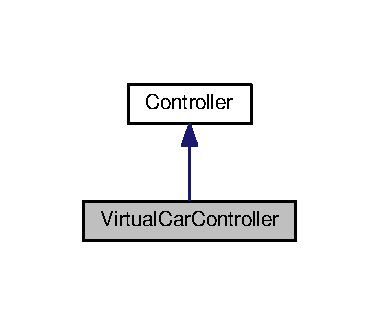
\includegraphics[width=182pt]{classVirtualCarController__inherit__graph}
\end{center}
\end{figure}


Collaboration diagram for Virtual\+Car\+Controller\+:\nopagebreak
\begin{figure}[H]
\begin{center}
\leavevmode
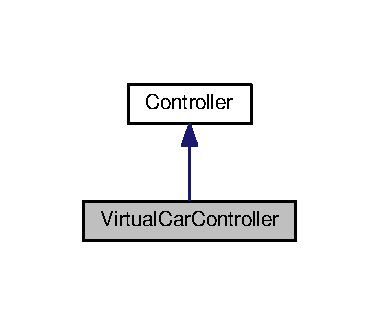
\includegraphics[width=182pt]{classVirtualCarController__coll__graph}
\end{center}
\end{figure}
\subsection*{Public Member Functions}
\begin{DoxyCompactItemize}
\item 
\hyperlink{classVirtualCarController_ac02bf679e405d1ea0b1c493bae0469ca}{Virtual\+Car\+Controller} ()
\item 
\hyperlink{Agent_8hpp_a5dd127bb3cb18b011cf5fd80a906e830}{Vector} \hyperlink{classVirtualCarController_acab2f4c5b7e8ef7ed5013058e6871fff}{update} (\hyperlink{Agent_8hpp_a5dd127bb3cb18b011cf5fd80a906e830}{Vector} input) override
\end{DoxyCompactItemize}
\subsection*{Additional Inherited Members}


\subsection{Detailed Description}
A \hyperlink{classVirtualCar}{Virtual\+Car} controller is the controller for the virtual car model (\hyperlink{classVirtualCarModel}{Virtual\+Car\+Model}) 

\subsection{Constructor \& Destructor Documentation}
\index{Virtual\+Car\+Controller@{Virtual\+Car\+Controller}!Virtual\+Car\+Controller@{Virtual\+Car\+Controller}}
\index{Virtual\+Car\+Controller@{Virtual\+Car\+Controller}!Virtual\+Car\+Controller@{Virtual\+Car\+Controller}}
\subsubsection[{\texorpdfstring{Virtual\+Car\+Controller()}{VirtualCarController()}}]{\setlength{\rightskip}{0pt plus 5cm}Virtual\+Car\+Controller\+::\+Virtual\+Car\+Controller (
\begin{DoxyParamCaption}
{}
\end{DoxyParamCaption}
)\hspace{0.3cm}{\ttfamily [explicit]}}\hypertarget{classVirtualCarController_ac02bf679e405d1ea0b1c493bae0469ca}{}\label{classVirtualCarController_ac02bf679e405d1ea0b1c493bae0469ca}
Constructor. Dimension of input vector is 3 (gas pedal, brake pedal, steering angle) Dimension of intermediate vector is 3. 

\subsection{Member Function Documentation}
\index{Virtual\+Car\+Controller@{Virtual\+Car\+Controller}!update@{update}}
\index{update@{update}!Virtual\+Car\+Controller@{Virtual\+Car\+Controller}}
\subsubsection[{\texorpdfstring{update(\+Vector input) override}{update(Vector input) override}}]{\setlength{\rightskip}{0pt plus 5cm}{\bf Vector} Virtual\+Car\+Controller\+::update (
\begin{DoxyParamCaption}
\item[{{\bf Vector}}]{input}
\end{DoxyParamCaption}
)\hspace{0.3cm}{\ttfamily [override]}, {\ttfamily [virtual]}}\hypertarget{classVirtualCarController_acab2f4c5b7e8ef7ed5013058e6871fff}{}\label{classVirtualCarController_acab2f4c5b7e8ef7ed5013058e6871fff}
Proportional controller. 
\begin{DoxyParams}{Parameters}
{\em input} & input vector (gas pedal, brake pedal, steering angle) \\
\hline
\end{DoxyParams}
\begin{DoxyReturn}{Returns}
intermediate vector which is empty. 
\end{DoxyReturn}


Implements \hyperlink{classController_acef11e408fb0d66d272bf5ab828cfbf6}{Controller}.



The documentation for this class was generated from the following files\+:\begin{DoxyCompactItemize}
\item 
Controllers/\hyperlink{VirtualCarController_8hpp}{Virtual\+Car\+Controller.\+hpp}\item 
Controllers/\hyperlink{VirtualCarController_8cpp}{Virtual\+Car\+Controller.\+cpp}\end{DoxyCompactItemize}

\hypertarget{classVirtualCarModel}{}\section{Virtual\+Car\+Model Class Reference}
\label{classVirtualCarModel}\index{Virtual\+Car\+Model@{Virtual\+Car\+Model}}


model for the virtual car  




{\ttfamily \#include $<$Virtual\+Car\+Model.\+hpp$>$}



Inheritance diagram for Virtual\+Car\+Model\+:\nopagebreak
\begin{figure}[H]
\begin{center}
\leavevmode
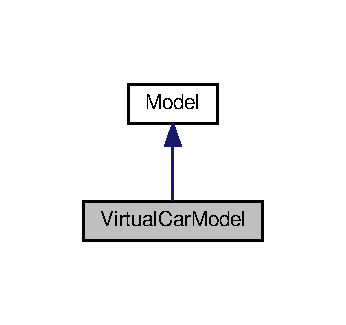
\includegraphics[width=166pt]{classVirtualCarModel__inherit__graph}
\end{center}
\end{figure}


Collaboration diagram for Virtual\+Car\+Model\+:\nopagebreak
\begin{figure}[H]
\begin{center}
\leavevmode
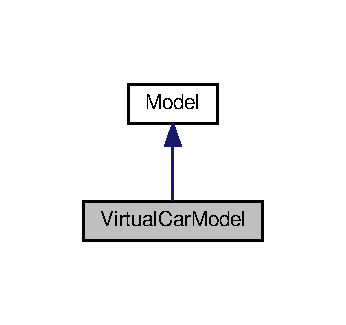
\includegraphics[width=166pt]{classVirtualCarModel__coll__graph}
\end{center}
\end{figure}
\subsection*{Public Member Functions}
\begin{DoxyCompactItemize}
\item 
\hyperlink{classVirtualCarModel_afc13c0d05e11bff23eb1b48402c5aa4a}{Virtual\+Car\+Model} ()
\item 
\hyperlink{Agent_8hpp_a5dd127bb3cb18b011cf5fd80a906e830}{Vector} \hyperlink{classVirtualCarModel_ab7a61fe2ce2180bd330dbf2819249457}{update} (\hyperlink{Agent_8hpp_a5dd127bb3cb18b011cf5fd80a906e830}{Vector} state, \hyperlink{Agent_8hpp_a5dd127bb3cb18b011cf5fd80a906e830}{Vector} intermediate) override
\end{DoxyCompactItemize}
\subsection*{Additional Inherited Members}


\subsection{Detailed Description}
model for the virtual car 

\subsection{Constructor \& Destructor Documentation}
\index{Virtual\+Car\+Model@{Virtual\+Car\+Model}!Virtual\+Car\+Model@{Virtual\+Car\+Model}}
\index{Virtual\+Car\+Model@{Virtual\+Car\+Model}!Virtual\+Car\+Model@{Virtual\+Car\+Model}}
\subsubsection[{\texorpdfstring{Virtual\+Car\+Model()}{VirtualCarModel()}}]{\setlength{\rightskip}{0pt plus 5cm}Virtual\+Car\+Model\+::\+Virtual\+Car\+Model (
\begin{DoxyParamCaption}
{}
\end{DoxyParamCaption}
)\hspace{0.3cm}{\ttfamily [explicit]}}\hypertarget{classVirtualCarModel_afc13c0d05e11bff23eb1b48402c5aa4a}{}\label{classVirtualCarModel_afc13c0d05e11bff23eb1b48402c5aa4a}
Constructor. Dimension of state vector is 6 (x, y, yaw, speed x, speed y, speed yaw) Dimension of intermediate vector is 3 (proportional to gas pedal, brake pedal, and steering angle) 

\subsection{Member Function Documentation}
\index{Virtual\+Car\+Model@{Virtual\+Car\+Model}!update@{update}}
\index{update@{update}!Virtual\+Car\+Model@{Virtual\+Car\+Model}}
\subsubsection[{\texorpdfstring{update(\+Vector state, Vector intermediate) override}{update(Vector state, Vector intermediate) override}}]{\setlength{\rightskip}{0pt plus 5cm}{\bf Vector} Virtual\+Car\+Model\+::update (
\begin{DoxyParamCaption}
\item[{{\bf Vector}}]{state, }
\item[{{\bf Vector}}]{intermediate}
\end{DoxyParamCaption}
)\hspace{0.3cm}{\ttfamily [override]}, {\ttfamily [virtual]}}\hypertarget{classVirtualCarModel_ab7a61fe2ce2180bd330dbf2819249457}{}\label{classVirtualCarModel_ab7a61fe2ce2180bd330dbf2819249457}
just return current state 
\begin{DoxyParams}{Parameters}
{\em state} & Dimension of state vector is 6 (x, y, yaw, speed x, speed y, speed yaw). \\
\hline
{\em intermediate} & Dimension of intermediate vector is 3 (proportional to gas pedal, brake pedal, and steering angle),which is empty and doesn\textquotesingle{}t be used. \\
\hline
\end{DoxyParams}
\begin{DoxyReturn}{Returns}
the state vector of this car for the next iteration 
\end{DoxyReturn}


Implements \hyperlink{classModel_a887e642d0c195b771af8300c7c817f09}{Model}.



The documentation for this class was generated from the following files\+:\begin{DoxyCompactItemize}
\item 
Models/\hyperlink{VirtualCarModel_8hpp}{Virtual\+Car\+Model.\+hpp}\item 
Models/\hyperlink{VirtualCarModel_8cpp}{Virtual\+Car\+Model.\+cpp}\end{DoxyCompactItemize}

\hypertarget{classVirtualCarPlanner}{}\section{Virtual\+Car\+Planner Class Reference}
\label{classVirtualCarPlanner}\index{Virtual\+Car\+Planner@{Virtual\+Car\+Planner}}


\hyperlink{classPlanner}{Planner} for the virtual car.  




{\ttfamily \#include $<$Virtual\+Car\+Planner.\+hpp$>$}



Inheritance diagram for Virtual\+Car\+Planner\+:\nopagebreak
\begin{figure}[H]
\begin{center}
\leavevmode
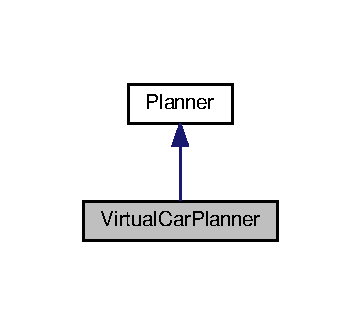
\includegraphics[width=173pt]{classVirtualCarPlanner__inherit__graph}
\end{center}
\end{figure}


Collaboration diagram for Virtual\+Car\+Planner\+:\nopagebreak
\begin{figure}[H]
\begin{center}
\leavevmode
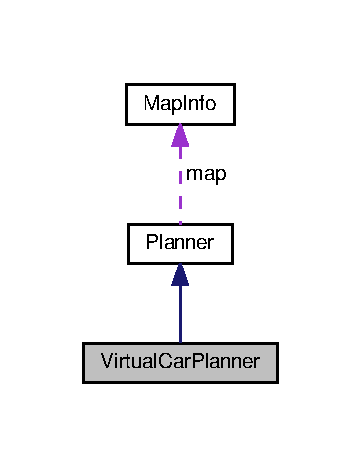
\includegraphics[width=173pt]{classVirtualCarPlanner__coll__graph}
\end{center}
\end{figure}
\subsection*{Public Member Functions}
\begin{DoxyCompactItemize}
\item 
\hyperlink{classVirtualCarPlanner_a9b60544002c9f51195a961036729f8a2}{Virtual\+Car\+Planner} ()
\item 
\hyperlink{Agent_8hpp_a5dd127bb3cb18b011cf5fd80a906e830}{Vector} \hyperlink{classVirtualCarPlanner_aa8624e1c729ebe167ace773ed271b160}{update} (\hyperlink{Agent_8hpp_a5dd127bb3cb18b011cf5fd80a906e830}{Vector} current\+State, const \hyperlink{Agent_8hpp_a5dd127bb3cb18b011cf5fd80a906e830}{Vector} \&human\+Input, std\+::vector$<$ \hyperlink{classAgent}{Agent} $\ast$ $>$ agents) override
\end{DoxyCompactItemize}
\subsection*{Additional Inherited Members}


\subsection{Detailed Description}
\hyperlink{classPlanner}{Planner} for the virtual car. 

\subsection{Constructor \& Destructor Documentation}
\index{Virtual\+Car\+Planner@{Virtual\+Car\+Planner}!Virtual\+Car\+Planner@{Virtual\+Car\+Planner}}
\index{Virtual\+Car\+Planner@{Virtual\+Car\+Planner}!Virtual\+Car\+Planner@{Virtual\+Car\+Planner}}
\subsubsection[{\texorpdfstring{Virtual\+Car\+Planner()}{VirtualCarPlanner()}}]{\setlength{\rightskip}{0pt plus 5cm}Virtual\+Car\+Planner\+::\+Virtual\+Car\+Planner (
\begin{DoxyParamCaption}
{}
\end{DoxyParamCaption}
)\hspace{0.3cm}{\ttfamily [explicit]}}\hypertarget{classVirtualCarPlanner_a9b60544002c9f51195a961036729f8a2}{}\label{classVirtualCarPlanner_a9b60544002c9f51195a961036729f8a2}
Constructor. Dimension of state vector is 6 (x, y, yaw, speed x, speed y, speed yaw) Dimension of input vector is 3 (gas pedal, brake pedal, and steering angle) 

\subsection{Member Function Documentation}
\index{Virtual\+Car\+Planner@{Virtual\+Car\+Planner}!update@{update}}
\index{update@{update}!Virtual\+Car\+Planner@{Virtual\+Car\+Planner}}
\subsubsection[{\texorpdfstring{update(\+Vector current\+State, const Vector \&human\+Input, std\+::vector$<$ Agent $\ast$ $>$ agents) override}{update(Vector currentState, const Vector &humanInput, std::vector< Agent * > agents) override}}]{\setlength{\rightskip}{0pt plus 5cm}{\bf Vector} Virtual\+Car\+Planner\+::update (
\begin{DoxyParamCaption}
\item[{{\bf Vector}}]{current\+State, }
\item[{const {\bf Vector} \&}]{human\+Input, }
\item[{std\+::vector$<$ {\bf Agent} $\ast$ $>$}]{agents}
\end{DoxyParamCaption}
)\hspace{0.3cm}{\ttfamily [override]}, {\ttfamily [virtual]}}\hypertarget{classVirtualCarPlanner_aa8624e1c729ebe167ace773ed271b160}{}\label{classVirtualCarPlanner_aa8624e1c729ebe167ace773ed271b160}
just returen a empty vector. 
\begin{DoxyParams}{Parameters}
{\em current\+State} & current state of the car. Doesn\textquotesingle{}t be used \\
\hline
{\em human\+Input} & current human input vector (gas pedal, brake pedal, and steering angle). Empty and doesn\textquotesingle{}t be used \\
\hline
{\em agents} & information of all agents in the simulator. Doesn\textquotesingle{}t be used \\
\hline
\end{DoxyParams}
\begin{DoxyReturn}{Returns}
empty vector,since the virtual car\textquotesingle{}s state is coming form .txt file or calculation. 
\end{DoxyReturn}


Implements \hyperlink{classPlanner_a62e1434402a3f36b0883e069a10447d8}{Planner}.



The documentation for this class was generated from the following files\+:\begin{DoxyCompactItemize}
\item 
Planners/\hyperlink{VirtualCarPlanner_8hpp}{Virtual\+Car\+Planner.\+hpp}\item 
Planners/\hyperlink{VirtualCarPlanner_8cpp}{Virtual\+Car\+Planner.\+cpp}\end{DoxyCompactItemize}

\chapter{File Documentation}
\hypertarget{Agent_8cpp}{}\section{Agents/\+Agent.cpp File Reference}
\label{Agent_8cpp}\index{Agents/\+Agent.\+cpp@{Agents/\+Agent.\+cpp}}
{\ttfamily \#include \char`\"{}Agent.\+hpp\char`\"{}}\\*
{\ttfamily \#include \char`\"{}../\+Simulator/\+Simulator.\+hpp\char`\"{}}\\*
{\ttfamily \#include $<$stdexcept$>$}\\*
{\ttfamily \#include $<$iostream$>$}\\*
{\ttfamily \#include $<$fstream$>$}\\*
Include dependency graph for Agent.\+cpp\+:
\nopagebreak
\begin{figure}[H]
\begin{center}
\leavevmode
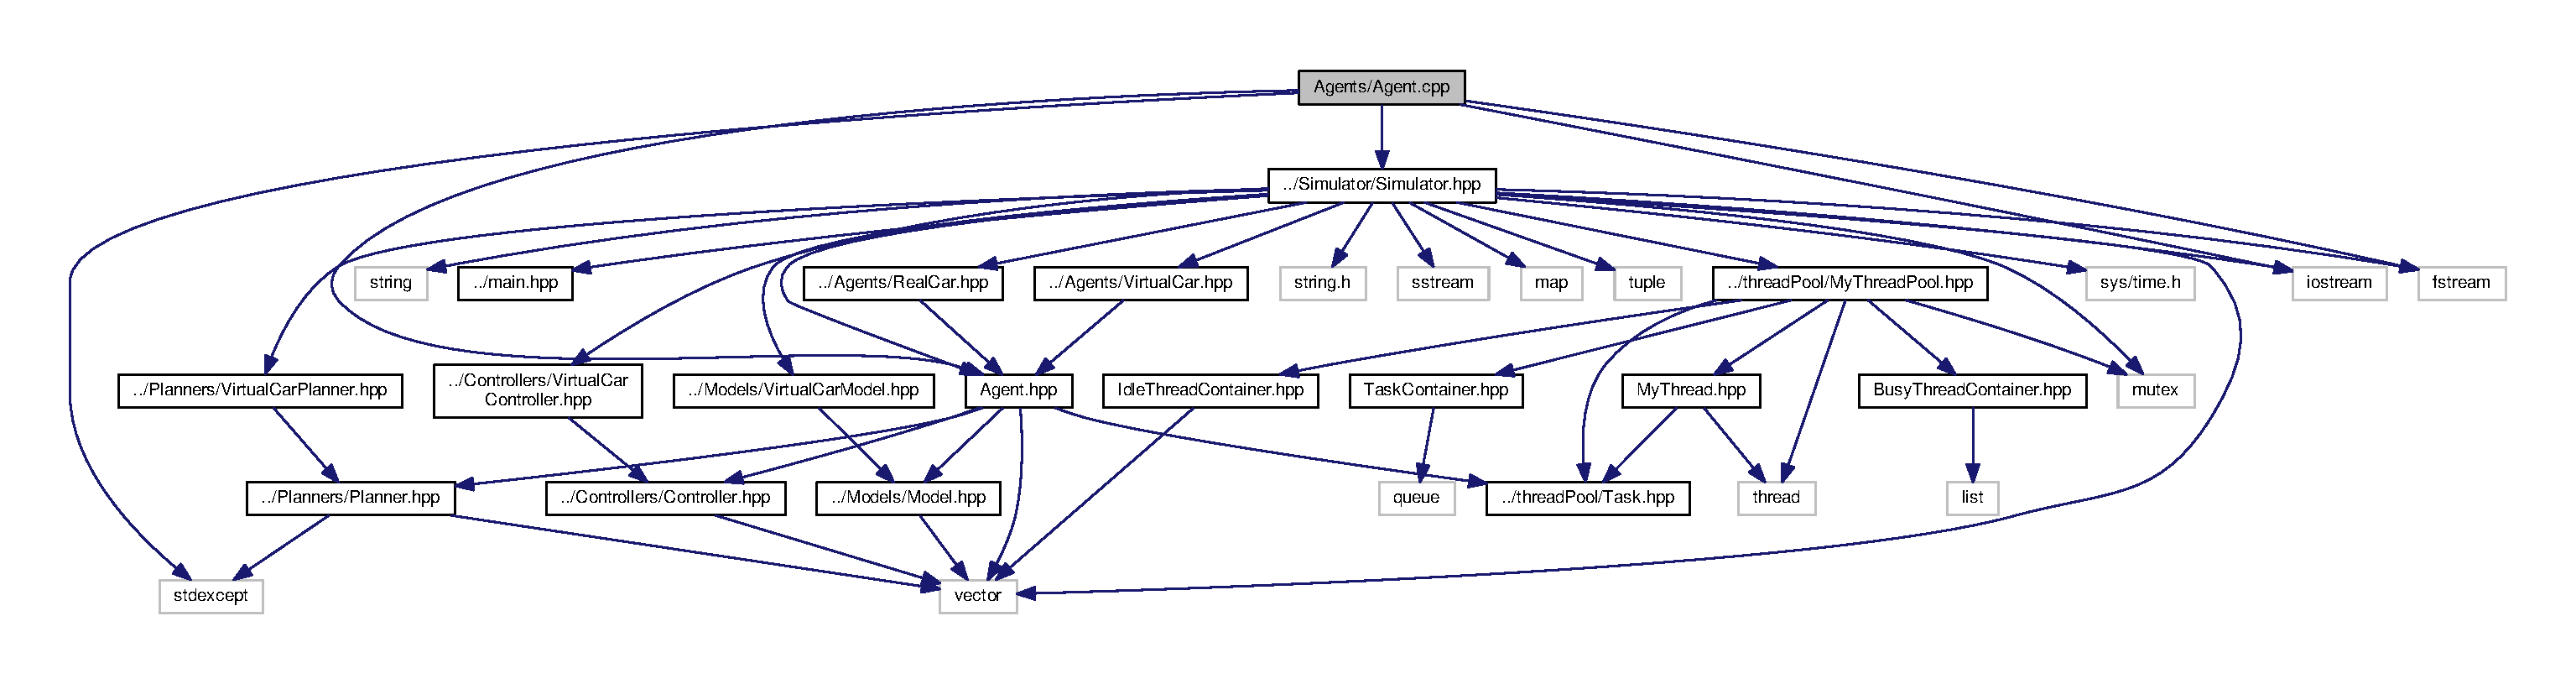
\includegraphics[width=350pt]{Agent_8cpp__incl}
\end{center}
\end{figure}

\hypertarget{Agent_8hpp}{}\section{Agents/\+Agent.hpp File Reference}
\label{Agent_8hpp}\index{Agents/\+Agent.\+hpp@{Agents/\+Agent.\+hpp}}
{\ttfamily \#include $<$vector$>$}\\*
{\ttfamily \#include \char`\"{}../thread\+Pool/\+Task.\+hpp\char`\"{}}\\*
{\ttfamily \#include \char`\"{}../\+Planners/\+Planner.\+hpp\char`\"{}}\\*
{\ttfamily \#include \char`\"{}../\+Controllers/\+Controller.\+hpp\char`\"{}}\\*
{\ttfamily \#include \char`\"{}../\+Models/\+Model.\+hpp\char`\"{}}\\*
Include dependency graph for Agent.\+hpp\+:
\nopagebreak
\begin{figure}[H]
\begin{center}
\leavevmode
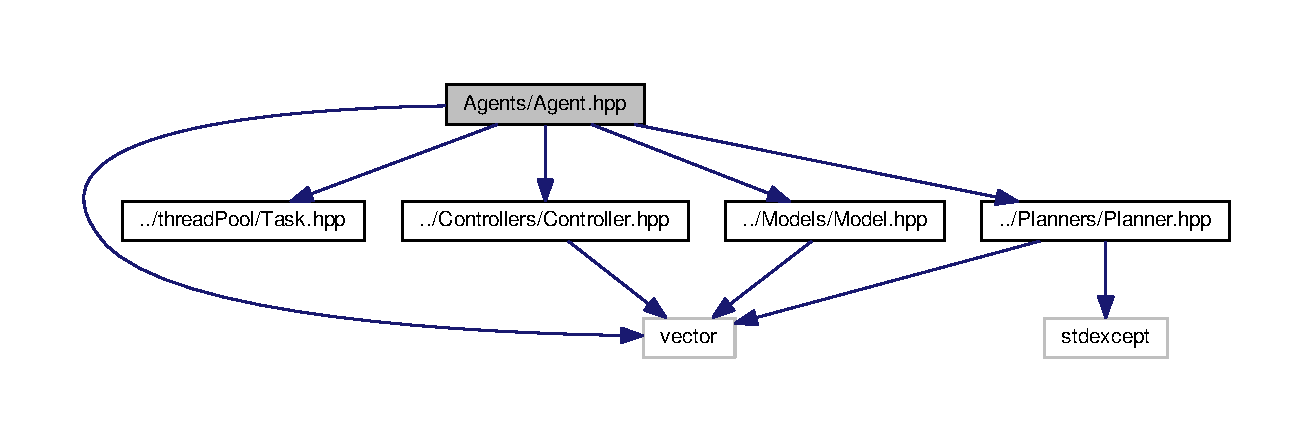
\includegraphics[width=350pt]{Agent_8hpp__incl}
\end{center}
\end{figure}
This graph shows which files directly or indirectly include this file\+:
\nopagebreak
\begin{figure}[H]
\begin{center}
\leavevmode
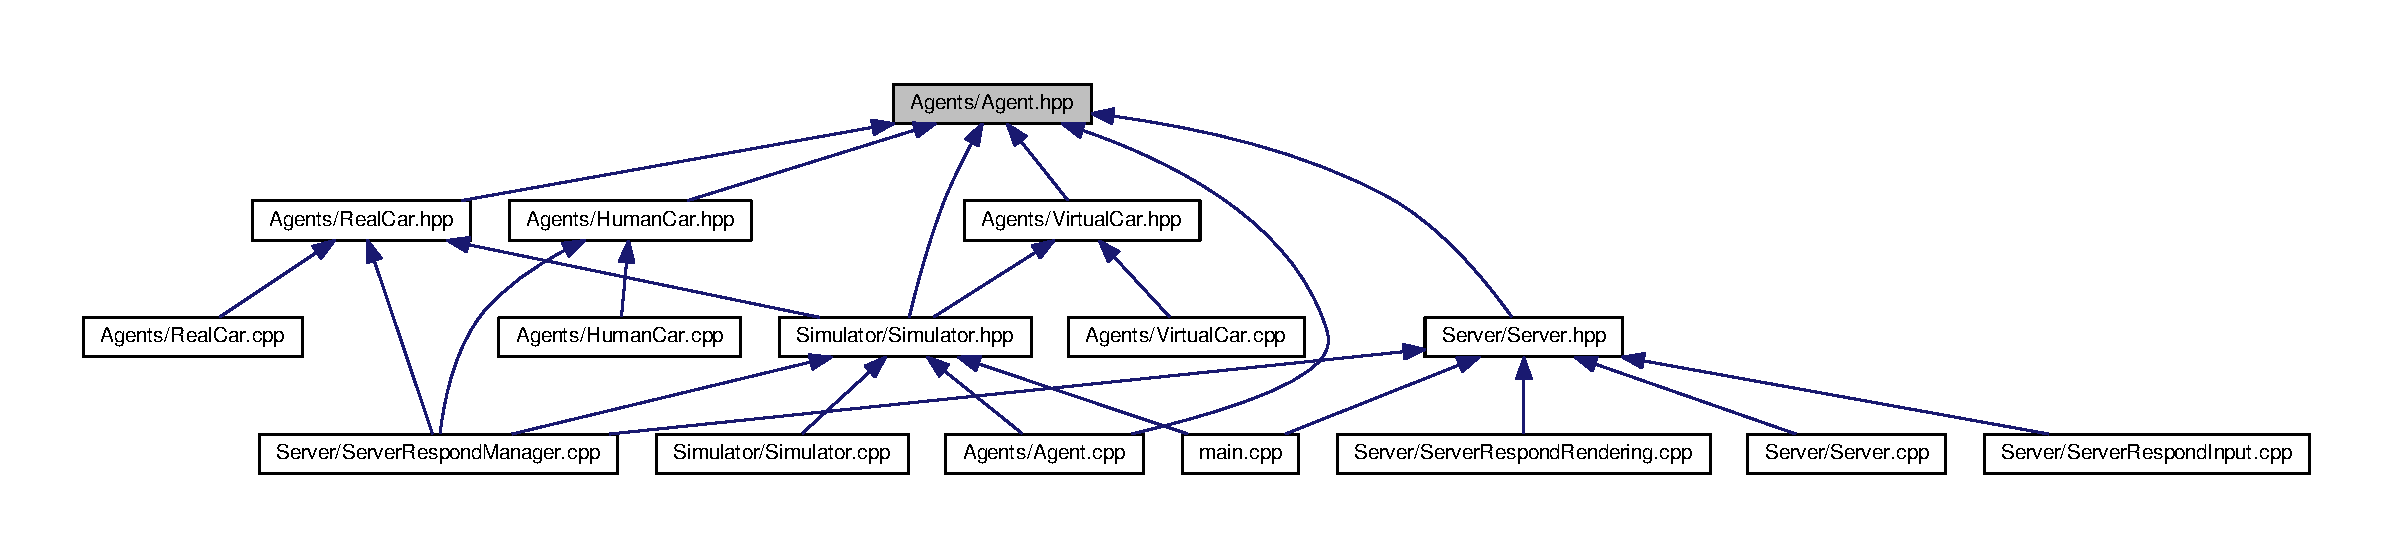
\includegraphics[width=350pt]{Agent_8hpp__dep__incl}
\end{center}
\end{figure}
\subsection*{Classes}
\begin{DoxyCompactItemize}
\item 
class \hyperlink{classAgent}{Agent}
\begin{DoxyCompactList}\small\item\em The parent class of all agents. An agent has a state vector and an id. \end{DoxyCompactList}\end{DoxyCompactItemize}
\subsection*{Typedefs}
\begin{DoxyCompactItemize}
\item 
typedef std\+::vector$<$ double $>$ \hyperlink{Agent_8hpp_a5dd127bb3cb18b011cf5fd80a906e830}{Vector}
\end{DoxyCompactItemize}
\subsection*{Enumerations}
\begin{DoxyCompactItemize}
\item 
enum \hyperlink{Agent_8hpp_ad2c3439c0fbb853c45129639d2581c51}{Agent\+Type} \{ \hyperlink{Agent_8hpp_ad2c3439c0fbb853c45129639d2581c51a633155c7db3760bd0ebdd9dbdc93f7f7}{Human\+Car} = 0, 
\hyperlink{Agent_8hpp_ad2c3439c0fbb853c45129639d2581c51a5a71f9a56b2d3f1b3cbab41f6d74527a}{Virtual\+Car} = 1, 
\hyperlink{Agent_8hpp_ad2c3439c0fbb853c45129639d2581c51a9c6a734fa0d0312984d2730bf4c1088c}{Real\+Car} = 2
 \}\begin{DoxyCompactList}\small\item\em This enumerator stands for the type of an agent. \end{DoxyCompactList}
\end{DoxyCompactItemize}


\subsection{Typedef Documentation}
\index{Agent.\+hpp@{Agent.\+hpp}!Vector@{Vector}}
\index{Vector@{Vector}!Agent.\+hpp@{Agent.\+hpp}}
\subsubsection[{\texorpdfstring{Vector}{Vector}}]{\setlength{\rightskip}{0pt plus 5cm}typedef std\+::vector$<$double$>$ {\bf Vector}}\hypertarget{Agent_8hpp_a5dd127bb3cb18b011cf5fd80a906e830}{}\label{Agent_8hpp_a5dd127bb3cb18b011cf5fd80a906e830}


\subsection{Enumeration Type Documentation}
\index{Agent.\+hpp@{Agent.\+hpp}!Agent\+Type@{Agent\+Type}}
\index{Agent\+Type@{Agent\+Type}!Agent.\+hpp@{Agent.\+hpp}}
\subsubsection[{\texorpdfstring{Agent\+Type}{AgentType}}]{\setlength{\rightskip}{0pt plus 5cm}enum {\bf Agent\+Type}}\hypertarget{Agent_8hpp_ad2c3439c0fbb853c45129639d2581c51}{}\label{Agent_8hpp_ad2c3439c0fbb853c45129639d2581c51}


This enumerator stands for the type of an agent. 

\begin{Desc}
\item[Enumerator]\par
\begin{description}
\index{Human\+Car@{Human\+Car}!Agent.\+hpp@{Agent.\+hpp}}\index{Agent.\+hpp@{Agent.\+hpp}!Human\+Car@{Human\+Car}}\item[{\em 
Human\+Car\hypertarget{Agent_8hpp_ad2c3439c0fbb853c45129639d2581c51a633155c7db3760bd0ebdd9dbdc93f7f7}{}\label{Agent_8hpp_ad2c3439c0fbb853c45129639d2581c51a633155c7db3760bd0ebdd9dbdc93f7f7}
}]\index{Virtual\+Car@{Virtual\+Car}!Agent.\+hpp@{Agent.\+hpp}}\index{Agent.\+hpp@{Agent.\+hpp}!Virtual\+Car@{Virtual\+Car}}\item[{\em 
Virtual\+Car\hypertarget{Agent_8hpp_ad2c3439c0fbb853c45129639d2581c51a5a71f9a56b2d3f1b3cbab41f6d74527a}{}\label{Agent_8hpp_ad2c3439c0fbb853c45129639d2581c51a5a71f9a56b2d3f1b3cbab41f6d74527a}
}]\index{Real\+Car@{Real\+Car}!Agent.\+hpp@{Agent.\+hpp}}\index{Agent.\+hpp@{Agent.\+hpp}!Real\+Car@{Real\+Car}}\item[{\em 
Real\+Car\hypertarget{Agent_8hpp_ad2c3439c0fbb853c45129639d2581c51a9c6a734fa0d0312984d2730bf4c1088c}{}\label{Agent_8hpp_ad2c3439c0fbb853c45129639d2581c51a9c6a734fa0d0312984d2730bf4c1088c}
}]\end{description}
\end{Desc}

\hypertarget{HumanCar_8cpp}{}\section{Agents/\+Human\+Car.cpp File Reference}
\label{HumanCar_8cpp}\index{Agents/\+Human\+Car.\+cpp@{Agents/\+Human\+Car.\+cpp}}
{\ttfamily \#include \char`\"{}Human\+Car.\+hpp\char`\"{}}\\*
Include dependency graph for Human\+Car.\+cpp\+:
\nopagebreak
\begin{figure}[H]
\begin{center}
\leavevmode
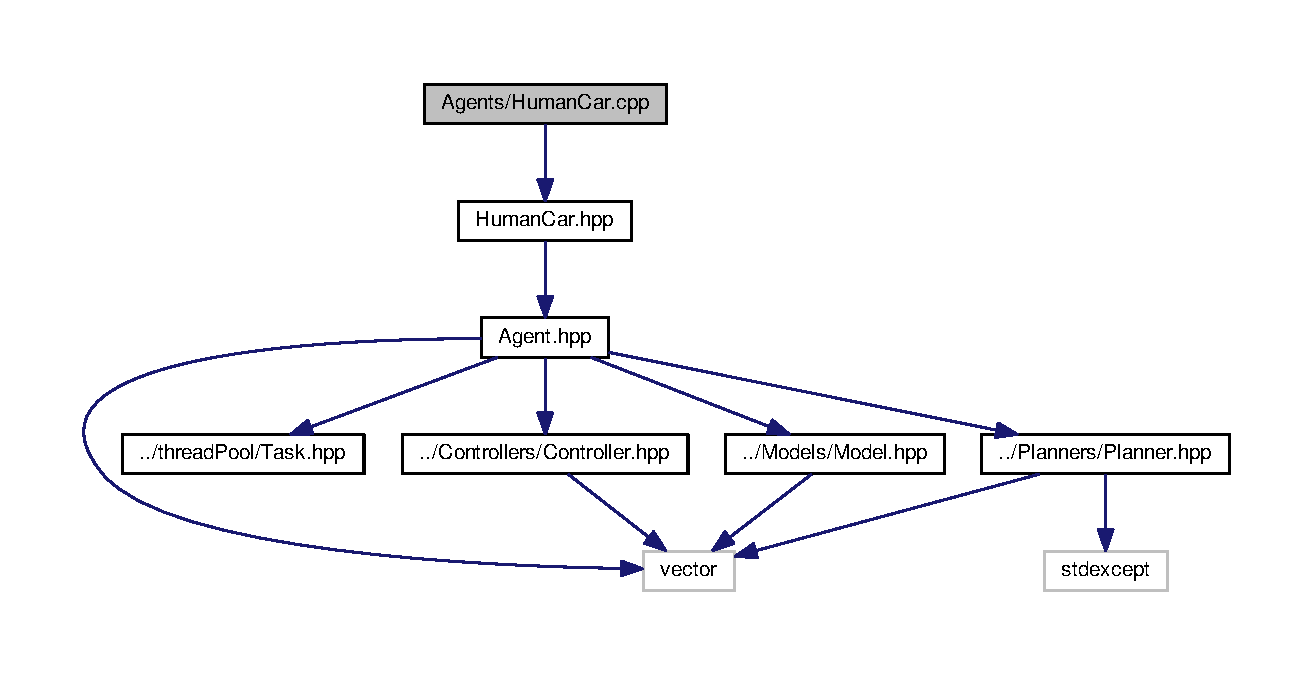
\includegraphics[width=350pt]{HumanCar_8cpp__incl}
\end{center}
\end{figure}

\hypertarget{HumanCar_8hpp}{}\section{Agents/\+Human\+Car.hpp File Reference}
\label{HumanCar_8hpp}\index{Agents/\+Human\+Car.\+hpp@{Agents/\+Human\+Car.\+hpp}}
{\ttfamily \#include \char`\"{}Agent.\+hpp\char`\"{}}\\*
Include dependency graph for Human\+Car.\+hpp\+:
\nopagebreak
\begin{figure}[H]
\begin{center}
\leavevmode
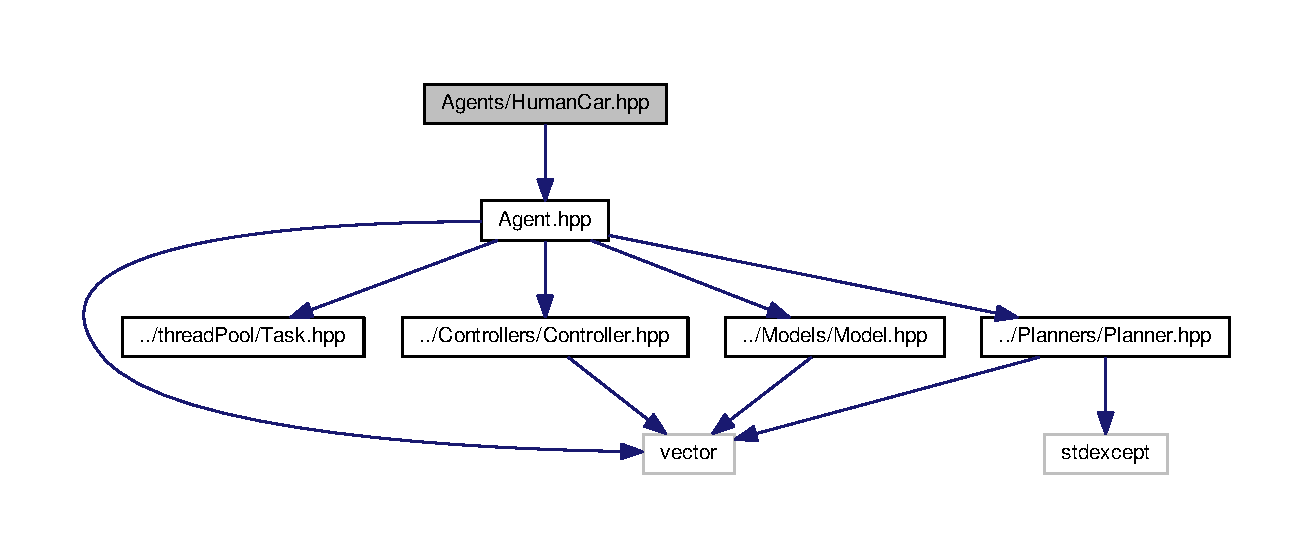
\includegraphics[width=350pt]{HumanCar_8hpp__incl}
\end{center}
\end{figure}
This graph shows which files directly or indirectly include this file\+:
\nopagebreak
\begin{figure}[H]
\begin{center}
\leavevmode
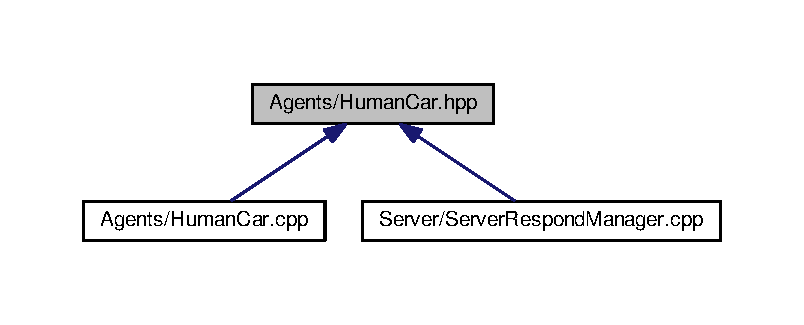
\includegraphics[width=350pt]{HumanCar_8hpp__dep__incl}
\end{center}
\end{figure}
\subsection*{Classes}
\begin{DoxyCompactItemize}
\item 
class \hyperlink{classHumanCar}{Human\+Car}
\end{DoxyCompactItemize}

\hypertarget{RealCar_8cpp}{}\section{Agents/\+Real\+Car.cpp File Reference}
\label{RealCar_8cpp}\index{Agents/\+Real\+Car.\+cpp@{Agents/\+Real\+Car.\+cpp}}
{\ttfamily \#include \char`\"{}Real\+Car.\+hpp\char`\"{}}\\*
Include dependency graph for Real\+Car.\+cpp\+:
\nopagebreak
\begin{figure}[H]
\begin{center}
\leavevmode
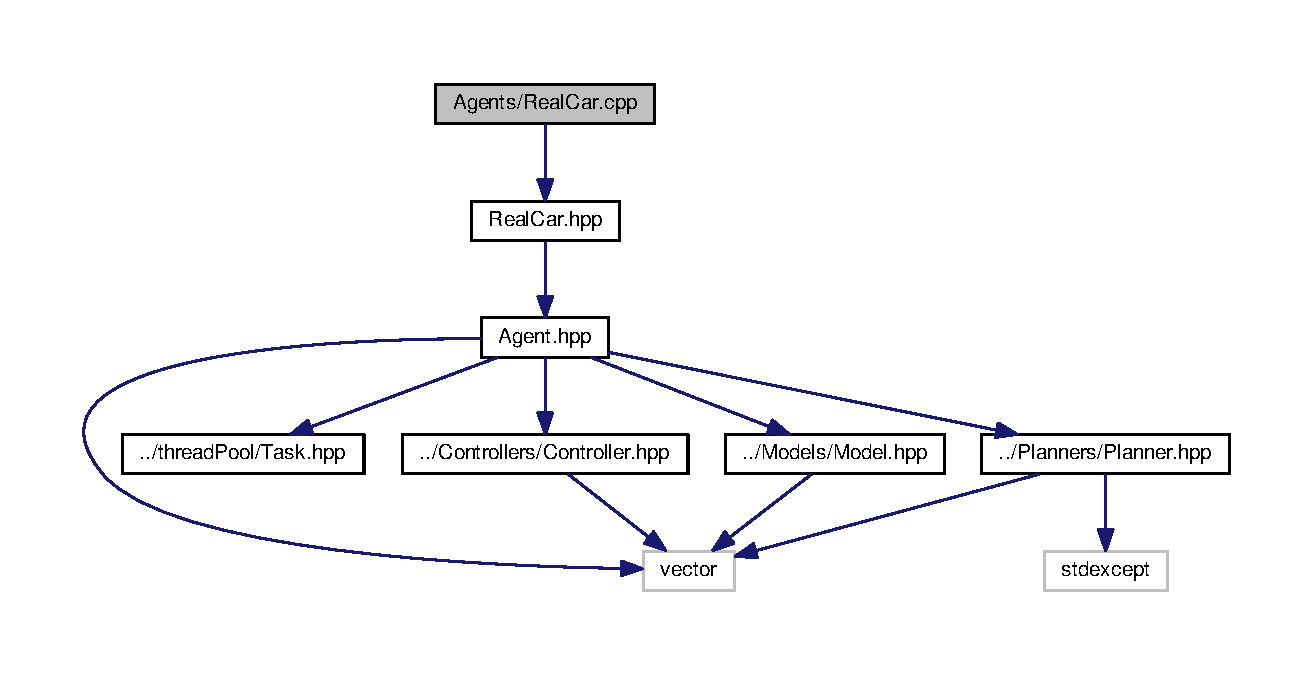
\includegraphics[width=350pt]{RealCar_8cpp__incl}
\end{center}
\end{figure}

\hypertarget{RealCar_8hpp}{}\section{Agents/\+Real\+Car.hpp File Reference}
\label{RealCar_8hpp}\index{Agents/\+Real\+Car.\+hpp@{Agents/\+Real\+Car.\+hpp}}
{\ttfamily \#include \char`\"{}Agent.\+hpp\char`\"{}}\\*
Include dependency graph for Real\+Car.\+hpp\+:
\nopagebreak
\begin{figure}[H]
\begin{center}
\leavevmode
\includegraphics[width=350pt]{RealCar_8hpp__incl}
\end{center}
\end{figure}
This graph shows which files directly or indirectly include this file\+:
\nopagebreak
\begin{figure}[H]
\begin{center}
\leavevmode
\includegraphics[width=350pt]{RealCar_8hpp__dep__incl}
\end{center}
\end{figure}
\subsection*{Classes}
\begin{DoxyCompactItemize}
\item 
class \hyperlink{classRealCar}{Real\+Car}
\end{DoxyCompactItemize}

\hypertarget{VirtualCar_8cpp}{}\section{Agents/\+Virtual\+Car.cpp File Reference}
\label{VirtualCar_8cpp}\index{Agents/\+Virtual\+Car.\+cpp@{Agents/\+Virtual\+Car.\+cpp}}
{\ttfamily \#include \char`\"{}Virtual\+Car.\+hpp\char`\"{}}\\*
Include dependency graph for Virtual\+Car.\+cpp\+:
\nopagebreak
\begin{figure}[H]
\begin{center}
\leavevmode
\includegraphics[width=350pt]{VirtualCar_8cpp__incl}
\end{center}
\end{figure}

\hypertarget{VirtualCar_8hpp}{}\section{Agents/\+Virtual\+Car.hpp File Reference}
\label{VirtualCar_8hpp}\index{Agents/\+Virtual\+Car.\+hpp@{Agents/\+Virtual\+Car.\+hpp}}
{\ttfamily \#include \char`\"{}Agent.\+hpp\char`\"{}}\\*
Include dependency graph for Virtual\+Car.\+hpp\+:
\nopagebreak
\begin{figure}[H]
\begin{center}
\leavevmode
\includegraphics[width=350pt]{VirtualCar_8hpp__incl}
\end{center}
\end{figure}
This graph shows which files directly or indirectly include this file\+:
\nopagebreak
\begin{figure}[H]
\begin{center}
\leavevmode
\includegraphics[width=350pt]{VirtualCar_8hpp__dep__incl}
\end{center}
\end{figure}
\subsection*{Classes}
\begin{DoxyCompactItemize}
\item 
class \hyperlink{classVirtualCar}{Virtual\+Car}
\end{DoxyCompactItemize}

\hypertarget{Controller_8cpp}{}\section{Controllers/\+Controller.cpp File Reference}
\label{Controller_8cpp}\index{Controllers/\+Controller.\+cpp@{Controllers/\+Controller.\+cpp}}
{\ttfamily \#include \char`\"{}Controller.\+hpp\char`\"{}}\\*
Include dependency graph for Controller.\+cpp\+:
\nopagebreak
\begin{figure}[H]
\begin{center}
\leavevmode
\includegraphics[width=208pt]{Controller_8cpp__incl}
\end{center}
\end{figure}

\hypertarget{Controller_8hpp}{}\section{Controllers/\+Controller.hpp File Reference}
\label{Controller_8hpp}\index{Controllers/\+Controller.\+hpp@{Controllers/\+Controller.\+hpp}}
{\ttfamily \#include $<$vector$>$}\\*
Include dependency graph for Controller.\+hpp\+:
\nopagebreak
\begin{figure}[H]
\begin{center}
\leavevmode
\includegraphics[width=208pt]{Controller_8hpp__incl}
\end{center}
\end{figure}
This graph shows which files directly or indirectly include this file\+:
\nopagebreak
\begin{figure}[H]
\begin{center}
\leavevmode
\includegraphics[width=350pt]{Controller_8hpp__dep__incl}
\end{center}
\end{figure}
\subsection*{Classes}
\begin{DoxyCompactItemize}
\item 
class \hyperlink{classController}{Controller}
\begin{DoxyCompactList}\small\item\em Parent class of all controllers. \end{DoxyCompactList}\end{DoxyCompactItemize}
\subsection*{Typedefs}
\begin{DoxyCompactItemize}
\item 
typedef std\+::vector$<$ double $>$ \hyperlink{Controller_8hpp_a5dd127bb3cb18b011cf5fd80a906e830}{Vector}
\end{DoxyCompactItemize}


\subsection{Typedef Documentation}
\index{Controller.\+hpp@{Controller.\+hpp}!Vector@{Vector}}
\index{Vector@{Vector}!Controller.\+hpp@{Controller.\+hpp}}
\subsubsection[{\texorpdfstring{Vector}{Vector}}]{\setlength{\rightskip}{0pt plus 5cm}typedef std\+::vector$<$double$>$ {\bf Vector}}\hypertarget{Controller_8hpp_a5dd127bb3cb18b011cf5fd80a906e830}{}\label{Controller_8hpp_a5dd127bb3cb18b011cf5fd80a906e830}

\hypertarget{FourWheelController_8cpp}{}\section{Controllers/\+Four\+Wheel\+Controller.cpp File Reference}
\label{FourWheelController_8cpp}\index{Controllers/\+Four\+Wheel\+Controller.\+cpp@{Controllers/\+Four\+Wheel\+Controller.\+cpp}}
{\ttfamily \#include \char`\"{}Four\+Wheel\+Controller.\+hpp\char`\"{}}\\*
{\ttfamily \#include $<$stdexcept$>$}\\*
{\ttfamily \#include $<$iostream$>$}\\*
Include dependency graph for Four\+Wheel\+Controller.\+cpp\+:
\nopagebreak
\begin{figure}[H]
\begin{center}
\leavevmode
\includegraphics[width=350pt]{FourWheelController_8cpp__incl}
\end{center}
\end{figure}

\hypertarget{FourWheelController_8hpp}{}\section{Controllers/\+Four\+Wheel\+Controller.hpp File Reference}
\label{FourWheelController_8hpp}\index{Controllers/\+Four\+Wheel\+Controller.\+hpp@{Controllers/\+Four\+Wheel\+Controller.\+hpp}}
{\ttfamily \#include \char`\"{}Controller.\+hpp\char`\"{}}\\*
Include dependency graph for Four\+Wheel\+Controller.\+hpp\+:
\nopagebreak
\begin{figure}[H]
\begin{center}
\leavevmode
\includegraphics[width=255pt]{FourWheelController_8hpp__incl}
\end{center}
\end{figure}
This graph shows which files directly or indirectly include this file\+:
\nopagebreak
\begin{figure}[H]
\begin{center}
\leavevmode
\includegraphics[width=350pt]{FourWheelController_8hpp__dep__incl}
\end{center}
\end{figure}
\subsection*{Classes}
\begin{DoxyCompactItemize}
\item 
class \hyperlink{classFourWheelController}{Four\+Wheel\+Controller}
\begin{DoxyCompactList}\small\item\em A four-\/wheel controller is the controller for the complex car model (\hyperlink{classFourWheelModel}{Four\+Wheel\+Model}) \end{DoxyCompactList}\end{DoxyCompactItemize}

\hypertarget{HumanCarController_8cpp}{}\section{Controllers/\+Human\+Car\+Controller.cpp File Reference}
\label{HumanCarController_8cpp}\index{Controllers/\+Human\+Car\+Controller.\+cpp@{Controllers/\+Human\+Car\+Controller.\+cpp}}
{\ttfamily \#include \char`\"{}Human\+Car\+Controller.\+hpp\char`\"{}}\\*
{\ttfamily \#include $<$stdexcept$>$}\\*
Include dependency graph for Human\+Car\+Controller.\+cpp\+:
\nopagebreak
\begin{figure}[H]
\begin{center}
\leavevmode
\includegraphics[width=285pt]{HumanCarController_8cpp__incl}
\end{center}
\end{figure}

\hypertarget{HumanCarController_8hpp}{}\section{Controllers/\+Human\+Car\+Controller.hpp File Reference}
\label{HumanCarController_8hpp}\index{Controllers/\+Human\+Car\+Controller.\+hpp@{Controllers/\+Human\+Car\+Controller.\+hpp}}
{\ttfamily \#include \char`\"{}Controller.\+hpp\char`\"{}}\\*
Include dependency graph for Human\+Car\+Controller.\+hpp\+:
\nopagebreak
\begin{figure}[H]
\begin{center}
\leavevmode
\includegraphics[width=255pt]{HumanCarController_8hpp__incl}
\end{center}
\end{figure}
This graph shows which files directly or indirectly include this file\+:
\nopagebreak
\begin{figure}[H]
\begin{center}
\leavevmode
\includegraphics[width=350pt]{HumanCarController_8hpp__dep__incl}
\end{center}
\end{figure}
\subsection*{Classes}
\begin{DoxyCompactItemize}
\item 
class \hyperlink{classHumanCarController}{Human\+Car\+Controller}
\begin{DoxyCompactList}\small\item\em A human car controller is the controller for the kinematic car model (\hyperlink{classHumanCarModel}{Human\+Car\+Model}) \end{DoxyCompactList}\end{DoxyCompactItemize}

\hypertarget{RealCarController_8cpp}{}\section{Controllers/\+Real\+Car\+Controller.cpp File Reference}
\label{RealCarController_8cpp}\index{Controllers/\+Real\+Car\+Controller.\+cpp@{Controllers/\+Real\+Car\+Controller.\+cpp}}
{\ttfamily \#include \char`\"{}Real\+Car\+Controller.\+hpp\char`\"{}}\\*
{\ttfamily \#include $<$stdexcept$>$}\\*
{\ttfamily \#include $<$iostream$>$}\\*
Include dependency graph for Real\+Car\+Controller.\+cpp\+:
\nopagebreak
\begin{figure}[H]
\begin{center}
\leavevmode
\includegraphics[width=343pt]{RealCarController_8cpp__incl}
\end{center}
\end{figure}

\hypertarget{RealCarController_8hpp}{}\section{Controllers/\+Real\+Car\+Controller.hpp File Reference}
\label{RealCarController_8hpp}\index{Controllers/\+Real\+Car\+Controller.\+hpp@{Controllers/\+Real\+Car\+Controller.\+hpp}}
{\ttfamily \#include \char`\"{}Controller.\+hpp\char`\"{}}\\*
Include dependency graph for Real\+Car\+Controller.\+hpp\+:
\nopagebreak
\begin{figure}[H]
\begin{center}
\leavevmode
\includegraphics[width=244pt]{RealCarController_8hpp__incl}
\end{center}
\end{figure}
This graph shows which files directly or indirectly include this file\+:
\nopagebreak
\begin{figure}[H]
\begin{center}
\leavevmode
\includegraphics[width=350pt]{RealCarController_8hpp__dep__incl}
\end{center}
\end{figure}
\subsection*{Classes}
\begin{DoxyCompactItemize}
\item 
class \hyperlink{classRealCarController}{Real\+Car\+Controller}
\begin{DoxyCompactList}\small\item\em A \hyperlink{classRealCar}{Real\+Car} controller is the controller for the real car model (\hyperlink{classRealCarModel}{Real\+Car\+Model}) \end{DoxyCompactList}\end{DoxyCompactItemize}

\hypertarget{SimplePidController_8cpp}{}\section{Controllers/\+Simple\+Pid\+Controller.cpp File Reference}
\label{SimplePidController_8cpp}\index{Controllers/\+Simple\+Pid\+Controller.\+cpp@{Controllers/\+Simple\+Pid\+Controller.\+cpp}}
{\ttfamily \#include \char`\"{}Simple\+Pid\+Controller.\+hpp\char`\"{}}\\*
{\ttfamily \#include \char`\"{}Pid\+Controller\+Lib/\+Pid\+Controller.\+h\char`\"{}}\\*
{\ttfamily \#include \char`\"{}../main.\+hpp\char`\"{}}\\*
Include dependency graph for Simple\+Pid\+Controller.\+cpp\+:
\nopagebreak
\begin{figure}[H]
\begin{center}
\leavevmode
\includegraphics[width=350pt]{SimplePidController_8cpp__incl}
\end{center}
\end{figure}
\subsection*{Macros}
\begin{DoxyCompactItemize}
\item 
\#define \hyperlink{SimplePidController_8cpp_addeef2b7cbeb36f285b2b8554212cf04}{P\+L\+A\+N\+\_\+\+S\+T\+EP}~(10)
\end{DoxyCompactItemize}


\subsection{Macro Definition Documentation}
\index{Simple\+Pid\+Controller.\+cpp@{Simple\+Pid\+Controller.\+cpp}!P\+L\+A\+N\+\_\+\+S\+T\+EP@{P\+L\+A\+N\+\_\+\+S\+T\+EP}}
\index{P\+L\+A\+N\+\_\+\+S\+T\+EP@{P\+L\+A\+N\+\_\+\+S\+T\+EP}!Simple\+Pid\+Controller.\+cpp@{Simple\+Pid\+Controller.\+cpp}}
\subsubsection[{\texorpdfstring{P\+L\+A\+N\+\_\+\+S\+T\+EP}{PLAN_STEP}}]{\setlength{\rightskip}{0pt plus 5cm}\#define P\+L\+A\+N\+\_\+\+S\+T\+EP~(10)}\hypertarget{SimplePidController_8cpp_addeef2b7cbeb36f285b2b8554212cf04}{}\label{SimplePidController_8cpp_addeef2b7cbeb36f285b2b8554212cf04}

\hypertarget{SimplePidController_8hpp}{}\section{Controllers/\+Simple\+Pid\+Controller.hpp File Reference}
\label{SimplePidController_8hpp}\index{Controllers/\+Simple\+Pid\+Controller.\+hpp@{Controllers/\+Simple\+Pid\+Controller.\+hpp}}
{\ttfamily \#include \char`\"{}Controller.\+hpp\char`\"{}}\\*
Include dependency graph for Simple\+Pid\+Controller.\+hpp\+:
\nopagebreak
\begin{figure}[H]
\begin{center}
\leavevmode
\includegraphics[width=252pt]{SimplePidController_8hpp__incl}
\end{center}
\end{figure}
This graph shows which files directly or indirectly include this file\+:
\nopagebreak
\begin{figure}[H]
\begin{center}
\leavevmode
\includegraphics[width=252pt]{SimplePidController_8hpp__dep__incl}
\end{center}
\end{figure}
\subsection*{Classes}
\begin{DoxyCompactItemize}
\item 
class \hyperlink{classSimplePidController}{Simple\+Pid\+Controller}
\begin{DoxyCompactList}\small\item\em A Simple\+Pid controller is the controller for the \hyperlink{classPlanner}{Planner} which may plan many step. \end{DoxyCompactList}\end{DoxyCompactItemize}

\hypertarget{VirtualCarController_8cpp}{}\section{Controllers/\+Virtual\+Car\+Controller.cpp File Reference}
\label{VirtualCarController_8cpp}\index{Controllers/\+Virtual\+Car\+Controller.\+cpp@{Controllers/\+Virtual\+Car\+Controller.\+cpp}}
{\ttfamily \#include \char`\"{}Virtual\+Car\+Controller.\+hpp\char`\"{}}\\*
{\ttfamily \#include $<$stdexcept$>$}\\*
{\ttfamily \#include $<$iostream$>$}\\*
Include dependency graph for Virtual\+Car\+Controller.\+cpp\+:
\nopagebreak
\begin{figure}[H]
\begin{center}
\leavevmode
\includegraphics[width=350pt]{VirtualCarController_8cpp__incl}
\end{center}
\end{figure}

\hypertarget{VirtualCarController_8hpp}{}\section{Controllers/\+Virtual\+Car\+Controller.hpp File Reference}
\label{VirtualCarController_8hpp}\index{Controllers/\+Virtual\+Car\+Controller.\+hpp@{Controllers/\+Virtual\+Car\+Controller.\+hpp}}
{\ttfamily \#include \char`\"{}Controller.\+hpp\char`\"{}}\\*
Include dependency graph for Virtual\+Car\+Controller.\+hpp\+:
\nopagebreak
\begin{figure}[H]
\begin{center}
\leavevmode
\includegraphics[width=251pt]{VirtualCarController_8hpp__incl}
\end{center}
\end{figure}
This graph shows which files directly or indirectly include this file\+:
\nopagebreak
\begin{figure}[H]
\begin{center}
\leavevmode
\includegraphics[width=350pt]{VirtualCarController_8hpp__dep__incl}
\end{center}
\end{figure}
\subsection*{Classes}
\begin{DoxyCompactItemize}
\item 
class \hyperlink{classVirtualCarController}{Virtual\+Car\+Controller}
\begin{DoxyCompactList}\small\item\em A \hyperlink{classVirtualCar}{Virtual\+Car} controller is the controller for the virtual car model (\hyperlink{classVirtualCarModel}{Virtual\+Car\+Model}) \end{DoxyCompactList}\end{DoxyCompactItemize}

\hypertarget{main_8cpp}{}\section{main.\+cpp File Reference}
\label{main_8cpp}\index{main.\+cpp@{main.\+cpp}}
{\ttfamily \#include $<$iostream$>$}\\*
{\ttfamily \#include \char`\"{}thread\+Pool/\+My\+Thread\+Pool.\+hpp\char`\"{}}\\*
{\ttfamily \#include \char`\"{}main.\+hpp\char`\"{}}\\*
{\ttfamily \#include \char`\"{}Server/\+Server.\+hpp\char`\"{}}\\*
{\ttfamily \#include \char`\"{}Simulator/\+Simulator.\+hpp\char`\"{}}\\*
Include dependency graph for main.\+cpp\+:
\nopagebreak
\begin{figure}[H]
\begin{center}
\leavevmode
\includegraphics[width=350pt]{main_8cpp__incl}
\end{center}
\end{figure}
\subsection*{Functions}
\begin{DoxyCompactItemize}
\item 
int \hyperlink{main_8cpp_ae66f6b31b5ad750f1fe042a706a4e3d4}{main} ()
\end{DoxyCompactItemize}


\subsection{Function Documentation}
\index{main.\+cpp@{main.\+cpp}!main@{main}}
\index{main@{main}!main.\+cpp@{main.\+cpp}}
\subsubsection[{\texorpdfstring{main()}{main()}}]{\setlength{\rightskip}{0pt plus 5cm}int main (
\begin{DoxyParamCaption}
{}
\end{DoxyParamCaption}
)}\hypertarget{main_8cpp_ae66f6b31b5ad750f1fe042a706a4e3d4}{}\label{main_8cpp_ae66f6b31b5ad750f1fe042a706a4e3d4}
Main function \begin{DoxyReturn}{Returns}

\end{DoxyReturn}

\hypertarget{main_8hpp}{}\section{main.\+hpp File Reference}
\label{main_8hpp}\index{main.\+hpp@{main.\+hpp}}
This graph shows which files directly or indirectly include this file\+:
\nopagebreak
\begin{figure}[H]
\begin{center}
\leavevmode
\includegraphics[width=350pt]{main_8hpp__dep__incl}
\end{center}
\end{figure}
\subsection*{Enumerations}
\begin{DoxyCompactItemize}
\item 
enum \hyperlink{main_8hpp_a4cb9f4bcd812094244f1949a88671bb8}{Simulator\+State} \{ \hyperlink{main_8hpp_a4cb9f4bcd812094244f1949a88671bb8a2f5f2c4a8c4f4f0519d503dcdfbf55cb}{Running} = 0, 
\hyperlink{main_8hpp_a4cb9f4bcd812094244f1949a88671bb8a7038380f2ccd1d2edf36a73fd4c2d068}{Paused} = 1, 
\hyperlink{main_8hpp_a4cb9f4bcd812094244f1949a88671bb8a92793663441ced378f4676b8a6524385}{Reset} = 2
 \}
\end{DoxyCompactItemize}
\subsection*{Variables}
\begin{DoxyCompactItemize}
\item 
const double \hyperlink{main_8hpp_acb9d9aec526b90f9353ec64c19e483b4}{S\+I\+M\+\_\+\+T\+I\+CK} = 0.\+01
\end{DoxyCompactItemize}


\subsection{Enumeration Type Documentation}
\index{main.\+hpp@{main.\+hpp}!Simulator\+State@{Simulator\+State}}
\index{Simulator\+State@{Simulator\+State}!main.\+hpp@{main.\+hpp}}
\subsubsection[{\texorpdfstring{Simulator\+State}{SimulatorState}}]{\setlength{\rightskip}{0pt plus 5cm}enum {\bf Simulator\+State}}\hypertarget{main_8hpp_a4cb9f4bcd812094244f1949a88671bb8}{}\label{main_8hpp_a4cb9f4bcd812094244f1949a88671bb8}
\begin{Desc}
\item[Enumerator]\par
\begin{description}
\index{Running@{Running}!main.\+hpp@{main.\+hpp}}\index{main.\+hpp@{main.\+hpp}!Running@{Running}}\item[{\em 
Running\hypertarget{main_8hpp_a4cb9f4bcd812094244f1949a88671bb8a2f5f2c4a8c4f4f0519d503dcdfbf55cb}{}\label{main_8hpp_a4cb9f4bcd812094244f1949a88671bb8a2f5f2c4a8c4f4f0519d503dcdfbf55cb}
}]\index{Paused@{Paused}!main.\+hpp@{main.\+hpp}}\index{main.\+hpp@{main.\+hpp}!Paused@{Paused}}\item[{\em 
Paused\hypertarget{main_8hpp_a4cb9f4bcd812094244f1949a88671bb8a7038380f2ccd1d2edf36a73fd4c2d068}{}\label{main_8hpp_a4cb9f4bcd812094244f1949a88671bb8a7038380f2ccd1d2edf36a73fd4c2d068}
}]\index{Reset@{Reset}!main.\+hpp@{main.\+hpp}}\index{main.\+hpp@{main.\+hpp}!Reset@{Reset}}\item[{\em 
Reset\hypertarget{main_8hpp_a4cb9f4bcd812094244f1949a88671bb8a92793663441ced378f4676b8a6524385}{}\label{main_8hpp_a4cb9f4bcd812094244f1949a88671bb8a92793663441ced378f4676b8a6524385}
}]\end{description}
\end{Desc}


\subsection{Variable Documentation}
\index{main.\+hpp@{main.\+hpp}!S\+I\+M\+\_\+\+T\+I\+CK@{S\+I\+M\+\_\+\+T\+I\+CK}}
\index{S\+I\+M\+\_\+\+T\+I\+CK@{S\+I\+M\+\_\+\+T\+I\+CK}!main.\+hpp@{main.\+hpp}}
\subsubsection[{\texorpdfstring{S\+I\+M\+\_\+\+T\+I\+CK}{SIM_TICK}}]{\setlength{\rightskip}{0pt plus 5cm}const double S\+I\+M\+\_\+\+T\+I\+CK = 0.\+01}\hypertarget{main_8hpp_acb9d9aec526b90f9353ec64c19e483b4}{}\label{main_8hpp_acb9d9aec526b90f9353ec64c19e483b4}

\hypertarget{MapInfo_8cpp}{}\section{Maps/\+Map\+Info.cpp File Reference}
\label{MapInfo_8cpp}\index{Maps/\+Map\+Info.\+cpp@{Maps/\+Map\+Info.\+cpp}}
{\ttfamily \#include \char`\"{}Map\+Info.\+hpp\char`\"{}}\\*
Include dependency graph for Map\+Info.\+cpp\+:
\nopagebreak
\begin{figure}[H]
\begin{center}
\leavevmode
\includegraphics[width=178pt]{MapInfo_8cpp__incl}
\end{center}
\end{figure}

\hypertarget{MapInfo_8hpp}{}\section{Maps/\+Map\+Info.hpp File Reference}
\label{MapInfo_8hpp}\index{Maps/\+Map\+Info.\+hpp@{Maps/\+Map\+Info.\+hpp}}
This graph shows which files directly or indirectly include this file\+:
\nopagebreak
\begin{figure}[H]
\begin{center}
\leavevmode
\includegraphics[width=178pt]{MapInfo_8hpp__dep__incl}
\end{center}
\end{figure}
\subsection*{Classes}
\begin{DoxyCompactItemize}
\item 
class \hyperlink{classMapInfo}{Map\+Info}
\begin{DoxyCompactList}\small\item\em this class is for read map. For now it is empty. \end{DoxyCompactList}\end{DoxyCompactItemize}

\hypertarget{FourWheelModel_8cpp}{}\section{Models/\+Four\+Wheel\+Model.cpp File Reference}
\label{FourWheelModel_8cpp}\index{Models/\+Four\+Wheel\+Model.\+cpp@{Models/\+Four\+Wheel\+Model.\+cpp}}
{\ttfamily \#include $<$iostream$>$}\\*
{\ttfamily \#include \char`\"{}Four\+Wheel\+Model.\+hpp\char`\"{}}\\*
{\ttfamily \#include \char`\"{}Four\+Wheel\+Model/\+Car\+\_\+4wheel.\+h\char`\"{}}\\*
Include dependency graph for Four\+Wheel\+Model.\+cpp\+:
\nopagebreak
\begin{figure}[H]
\begin{center}
\leavevmode
\includegraphics[width=350pt]{FourWheelModel_8cpp__incl}
\end{center}
\end{figure}

\hypertarget{FourWheelModel_8hpp}{}\section{Models/\+Four\+Wheel\+Model.hpp File Reference}
\label{FourWheelModel_8hpp}\index{Models/\+Four\+Wheel\+Model.\+hpp@{Models/\+Four\+Wheel\+Model.\+hpp}}
{\ttfamily \#include \char`\"{}Model.\+hpp\char`\"{}}\\*
Include dependency graph for Four\+Wheel\+Model.\+hpp\+:
\nopagebreak
\begin{figure}[H]
\begin{center}
\leavevmode
\includegraphics[width=223pt]{FourWheelModel_8hpp__incl}
\end{center}
\end{figure}
This graph shows which files directly or indirectly include this file\+:
\nopagebreak
\begin{figure}[H]
\begin{center}
\leavevmode
\includegraphics[width=350pt]{FourWheelModel_8hpp__dep__incl}
\end{center}
\end{figure}
\subsection*{Classes}
\begin{DoxyCompactItemize}
\item 
class \hyperlink{classFourWheelModel}{Four\+Wheel\+Model}
\begin{DoxyCompactList}\small\item\em Complex model for a human car. \end{DoxyCompactList}\end{DoxyCompactItemize}

\hypertarget{HumanCarModel_8cpp}{}\section{Models/\+Human\+Car\+Model.cpp File Reference}
\label{HumanCarModel_8cpp}\index{Models/\+Human\+Car\+Model.\+cpp@{Models/\+Human\+Car\+Model.\+cpp}}
{\ttfamily \#include \char`\"{}Human\+Car\+Model.\+hpp\char`\"{}}\\*
{\ttfamily \#include $<$stdexcept$>$}\\*
{\ttfamily \#include $<$cmath$>$}\\*
{\ttfamily \#include \char`\"{}../main.\+hpp\char`\"{}}\\*
Include dependency graph for Human\+Car\+Model.\+cpp\+:
\nopagebreak
\begin{figure}[H]
\begin{center}
\leavevmode
\includegraphics[width=350pt]{HumanCarModel_8cpp__incl}
\end{center}
\end{figure}

\hypertarget{HumanCarModel_8hpp}{}\section{Models/\+Human\+Car\+Model.hpp File Reference}
\label{HumanCarModel_8hpp}\index{Models/\+Human\+Car\+Model.\+hpp@{Models/\+Human\+Car\+Model.\+hpp}}
{\ttfamily \#include \char`\"{}Model.\+hpp\char`\"{}}\\*
Include dependency graph for Human\+Car\+Model.\+hpp\+:
\nopagebreak
\begin{figure}[H]
\begin{center}
\leavevmode
\includegraphics[width=223pt]{HumanCarModel_8hpp__incl}
\end{center}
\end{figure}
This graph shows which files directly or indirectly include this file\+:
\nopagebreak
\begin{figure}[H]
\begin{center}
\leavevmode
\includegraphics[width=350pt]{HumanCarModel_8hpp__dep__incl}
\end{center}
\end{figure}
\subsection*{Classes}
\begin{DoxyCompactItemize}
\item 
class \hyperlink{classHumanCarModel}{Human\+Car\+Model}
\begin{DoxyCompactList}\small\item\em Simple kinematic model for a human car. \end{DoxyCompactList}\end{DoxyCompactItemize}

\hypertarget{Model_8cpp}{}\section{Models/\+Model.cpp File Reference}
\label{Model_8cpp}\index{Models/\+Model.\+cpp@{Models/\+Model.\+cpp}}
{\ttfamily \#include \char`\"{}Model.\+hpp\char`\"{}}\\*
Include dependency graph for Model.\+cpp\+:
\nopagebreak
\begin{figure}[H]
\begin{center}
\leavevmode
\includegraphics[width=176pt]{Model_8cpp__incl}
\end{center}
\end{figure}

\hypertarget{Model_8hpp}{}\section{Models/\+Model.hpp File Reference}
\label{Model_8hpp}\index{Models/\+Model.\+hpp@{Models/\+Model.\+hpp}}
{\ttfamily \#include $<$vector$>$}\\*
Include dependency graph for Model.\+hpp\+:
\nopagebreak
\begin{figure}[H]
\begin{center}
\leavevmode
\includegraphics[width=176pt]{Model_8hpp__incl}
\end{center}
\end{figure}
This graph shows which files directly or indirectly include this file\+:
\nopagebreak
\begin{figure}[H]
\begin{center}
\leavevmode
\includegraphics[width=350pt]{Model_8hpp__dep__incl}
\end{center}
\end{figure}
\subsection*{Classes}
\begin{DoxyCompactItemize}
\item 
class \hyperlink{classModel}{Model}
\begin{DoxyCompactList}\small\item\em Parent class for all models. \end{DoxyCompactList}\end{DoxyCompactItemize}
\subsection*{Typedefs}
\begin{DoxyCompactItemize}
\item 
typedef std\+::vector$<$ double $>$ \hyperlink{Model_8hpp_a5dd127bb3cb18b011cf5fd80a906e830}{Vector}
\end{DoxyCompactItemize}


\subsection{Typedef Documentation}
\index{Model.\+hpp@{Model.\+hpp}!Vector@{Vector}}
\index{Vector@{Vector}!Model.\+hpp@{Model.\+hpp}}
\subsubsection[{\texorpdfstring{Vector}{Vector}}]{\setlength{\rightskip}{0pt plus 5cm}typedef std\+::vector$<$double$>$ {\bf Vector}}\hypertarget{Model_8hpp_a5dd127bb3cb18b011cf5fd80a906e830}{}\label{Model_8hpp_a5dd127bb3cb18b011cf5fd80a906e830}

\hypertarget{RealCarModel_8cpp}{}\section{Models/\+Real\+Car\+Model.cpp File Reference}
\label{RealCarModel_8cpp}\index{Models/\+Real\+Car\+Model.\+cpp@{Models/\+Real\+Car\+Model.\+cpp}}
{\ttfamily \#include \char`\"{}Real\+Car\+Model.\+hpp\char`\"{}}\\*
{\ttfamily \#include $<$iostream$>$}\\*
{\ttfamily \#include $<$fstream$>$}\\*
{\ttfamily \#include \char`\"{}Four\+Wheel\+Model/\+Car\+\_\+4wheel.\+h\char`\"{}}\\*
Include dependency graph for Real\+Car\+Model.\+cpp\+:
\nopagebreak
\begin{figure}[H]
\begin{center}
\leavevmode
\includegraphics[width=350pt]{RealCarModel_8cpp__incl}
\end{center}
\end{figure}

\hypertarget{RealCarModel_8hpp}{}\section{Models/\+Real\+Car\+Model.hpp File Reference}
\label{RealCarModel_8hpp}\index{Models/\+Real\+Car\+Model.\+hpp@{Models/\+Real\+Car\+Model.\+hpp}}
{\ttfamily \#include \char`\"{}Model.\+hpp\char`\"{}}\\*
Include dependency graph for Real\+Car\+Model.\+hpp\+:
\nopagebreak
\begin{figure}[H]
\begin{center}
\leavevmode
\includegraphics[width=212pt]{RealCarModel_8hpp__incl}
\end{center}
\end{figure}
This graph shows which files directly or indirectly include this file\+:
\nopagebreak
\begin{figure}[H]
\begin{center}
\leavevmode
\includegraphics[width=350pt]{RealCarModel_8hpp__dep__incl}
\end{center}
\end{figure}
\subsection*{Classes}
\begin{DoxyCompactItemize}
\item 
class \hyperlink{classRealCarModel}{Real\+Car\+Model}
\begin{DoxyCompactList}\small\item\em model for the real car \end{DoxyCompactList}\end{DoxyCompactItemize}

\hypertarget{VirtualCarModel_8cpp}{}\section{Models/\+Virtual\+Car\+Model.cpp File Reference}
\label{VirtualCarModel_8cpp}\index{Models/\+Virtual\+Car\+Model.\+cpp@{Models/\+Virtual\+Car\+Model.\+cpp}}
{\ttfamily \#include \char`\"{}Virtual\+Car\+Model.\+hpp\char`\"{}}\\*
Include dependency graph for Virtual\+Car\+Model.\+cpp\+:
\nopagebreak
\begin{figure}[H]
\begin{center}
\leavevmode
\includegraphics[width=220pt]{VirtualCarModel_8cpp__incl}
\end{center}
\end{figure}

\hypertarget{VirtualCarModel_8hpp}{}\section{Models/\+Virtual\+Car\+Model.hpp File Reference}
\label{VirtualCarModel_8hpp}\index{Models/\+Virtual\+Car\+Model.\+hpp@{Models/\+Virtual\+Car\+Model.\+hpp}}
{\ttfamily \#include \char`\"{}Model.\+hpp\char`\"{}}\\*
Include dependency graph for Virtual\+Car\+Model.\+hpp\+:
\nopagebreak
\begin{figure}[H]
\begin{center}
\leavevmode
\includegraphics[width=220pt]{VirtualCarModel_8hpp__incl}
\end{center}
\end{figure}
This graph shows which files directly or indirectly include this file\+:
\nopagebreak
\begin{figure}[H]
\begin{center}
\leavevmode
\includegraphics[width=350pt]{VirtualCarModel_8hpp__dep__incl}
\end{center}
\end{figure}
\subsection*{Classes}
\begin{DoxyCompactItemize}
\item 
class \hyperlink{classVirtualCarModel}{Virtual\+Car\+Model}
\begin{DoxyCompactList}\small\item\em model for the virtual car \end{DoxyCompactList}\end{DoxyCompactItemize}

\hypertarget{HumanCarPlanner_8cpp}{}\section{Planners/\+Human\+Car\+Planner.cpp File Reference}
\label{HumanCarPlanner_8cpp}\index{Planners/\+Human\+Car\+Planner.\+cpp@{Planners/\+Human\+Car\+Planner.\+cpp}}
{\ttfamily \#include \char`\"{}Human\+Car\+Planner.\+hpp\char`\"{}}\\*
{\ttfamily \#include $<$stdexcept$>$}\\*
Include dependency graph for Human\+Car\+Planner.\+cpp\+:
\nopagebreak
\begin{figure}[H]
\begin{center}
\leavevmode
\includegraphics[width=260pt]{HumanCarPlanner_8cpp__incl}
\end{center}
\end{figure}

\hypertarget{HumanCarPlanner_8hpp}{}\section{Planners/\+Human\+Car\+Planner.hpp File Reference}
\label{HumanCarPlanner_8hpp}\index{Planners/\+Human\+Car\+Planner.\+hpp@{Planners/\+Human\+Car\+Planner.\+hpp}}
{\ttfamily \#include \char`\"{}Planner.\+hpp\char`\"{}}\\*
Include dependency graph for Human\+Car\+Planner.\+hpp\+:
\nopagebreak
\begin{figure}[H]
\begin{center}
\leavevmode
\includegraphics[width=237pt]{HumanCarPlanner_8hpp__incl}
\end{center}
\end{figure}
This graph shows which files directly or indirectly include this file\+:
\nopagebreak
\begin{figure}[H]
\begin{center}
\leavevmode
\includegraphics[width=350pt]{HumanCarPlanner_8hpp__dep__incl}
\end{center}
\end{figure}
\subsection*{Classes}
\begin{DoxyCompactItemize}
\item 
class \hyperlink{classHumanCarPlanner}{Human\+Car\+Planner}
\begin{DoxyCompactList}\small\item\em \hyperlink{classPlanner}{Planner} for a human car, which passes human inputs directly. \end{DoxyCompactList}\end{DoxyCompactItemize}

\hypertarget{Planner_8cpp}{}\section{Planners/\+Planner.cpp File Reference}
\label{Planner_8cpp}\index{Planners/\+Planner.\+cpp@{Planners/\+Planner.\+cpp}}
{\ttfamily \#include \char`\"{}Planner.\+hpp\char`\"{}}\\*
Include dependency graph for Planner.\+cpp\+:
\nopagebreak
\begin{figure}[H]
\begin{center}
\leavevmode
\includegraphics[width=202pt]{Planner_8cpp__incl}
\end{center}
\end{figure}

\hypertarget{Planner_8hpp}{}\section{Planners/\+Planner.hpp File Reference}
\label{Planner_8hpp}\index{Planners/\+Planner.\+hpp@{Planners/\+Planner.\+hpp}}
{\ttfamily \#include $<$vector$>$}\\*
{\ttfamily \#include $<$stdexcept$>$}\\*
Include dependency graph for Planner.\+hpp\+:
\nopagebreak
\begin{figure}[H]
\begin{center}
\leavevmode
\includegraphics[width=202pt]{Planner_8hpp__incl}
\end{center}
\end{figure}
This graph shows which files directly or indirectly include this file\+:
\nopagebreak
\begin{figure}[H]
\begin{center}
\leavevmode
\includegraphics[width=350pt]{Planner_8hpp__dep__incl}
\end{center}
\end{figure}
\subsection*{Classes}
\begin{DoxyCompactItemize}
\item 
class \hyperlink{classPlanner}{Planner}
\begin{DoxyCompactList}\small\item\em Parent class for all planners. \end{DoxyCompactList}\end{DoxyCompactItemize}
\subsection*{Typedefs}
\begin{DoxyCompactItemize}
\item 
typedef std\+::vector$<$ double $>$ \hyperlink{Planner_8hpp_a5dd127bb3cb18b011cf5fd80a906e830}{Vector}
\end{DoxyCompactItemize}


\subsection{Typedef Documentation}
\index{Planner.\+hpp@{Planner.\+hpp}!Vector@{Vector}}
\index{Vector@{Vector}!Planner.\+hpp@{Planner.\+hpp}}
\subsubsection[{\texorpdfstring{Vector}{Vector}}]{\setlength{\rightskip}{0pt plus 5cm}typedef std\+::vector$<$double$>$ {\bf Vector}}\hypertarget{Planner_8hpp_a5dd127bb3cb18b011cf5fd80a906e830}{}\label{Planner_8hpp_a5dd127bb3cb18b011cf5fd80a906e830}

\hypertarget{RealCarPlanner_8cpp}{}\section{Planners/\+Real\+Car\+Planner.cpp File Reference}
\label{RealCarPlanner_8cpp}\index{Planners/\+Real\+Car\+Planner.\+cpp@{Planners/\+Real\+Car\+Planner.\+cpp}}
{\ttfamily \#include \char`\"{}Real\+Car\+Planner.\+hpp\char`\"{}}\\*
{\ttfamily \#include $<$stdexcept$>$}\\*
Include dependency graph for Real\+Car\+Planner.\+cpp\+:
\nopagebreak
\begin{figure}[H]
\begin{center}
\leavevmode
\includegraphics[width=245pt]{RealCarPlanner_8cpp__incl}
\end{center}
\end{figure}

\hypertarget{RealCarPlanner_8hpp}{}\section{Planners/\+Real\+Car\+Planner.hpp File Reference}
\label{RealCarPlanner_8hpp}\index{Planners/\+Real\+Car\+Planner.\+hpp@{Planners/\+Real\+Car\+Planner.\+hpp}}
{\ttfamily \#include \char`\"{}Planner.\+hpp\char`\"{}}\\*
Include dependency graph for Real\+Car\+Planner.\+hpp\+:
\nopagebreak
\begin{figure}[H]
\begin{center}
\leavevmode
\includegraphics[width=226pt]{RealCarPlanner_8hpp__incl}
\end{center}
\end{figure}
This graph shows which files directly or indirectly include this file\+:
\nopagebreak
\begin{figure}[H]
\begin{center}
\leavevmode
\includegraphics[width=350pt]{RealCarPlanner_8hpp__dep__incl}
\end{center}
\end{figure}
\subsection*{Classes}
\begin{DoxyCompactItemize}
\item 
class \hyperlink{classRealCarPlanner}{Real\+Car\+Planner}
\begin{DoxyCompactList}\small\item\em \hyperlink{classPlanner}{Planner} for the real car. \end{DoxyCompactList}\end{DoxyCompactItemize}

\hypertarget{TrivialPlanner_8cpp}{}\section{Planners/\+Trivial\+Planner.cpp File Reference}
\label{TrivialPlanner_8cpp}\index{Planners/\+Trivial\+Planner.\+cpp@{Planners/\+Trivial\+Planner.\+cpp}}
{\ttfamily \#include \char`\"{}Trivial\+Planner.\+hpp\char`\"{}}\\*
{\ttfamily \#include $<$cmath$>$}\\*
Include dependency graph for Trivial\+Planner.\+cpp\+:
\nopagebreak
\begin{figure}[H]
\begin{center}
\leavevmode
\includegraphics[width=249pt]{TrivialPlanner_8cpp__incl}
\end{center}
\end{figure}
\subsection*{Macros}
\begin{DoxyCompactItemize}
\item 
\#define \hyperlink{TrivialPlanner_8cpp_addeef2b7cbeb36f285b2b8554212cf04}{P\+L\+A\+N\+\_\+\+S\+T\+EP}~(10)
\end{DoxyCompactItemize}


\subsection{Macro Definition Documentation}
\index{Trivial\+Planner.\+cpp@{Trivial\+Planner.\+cpp}!P\+L\+A\+N\+\_\+\+S\+T\+EP@{P\+L\+A\+N\+\_\+\+S\+T\+EP}}
\index{P\+L\+A\+N\+\_\+\+S\+T\+EP@{P\+L\+A\+N\+\_\+\+S\+T\+EP}!Trivial\+Planner.\+cpp@{Trivial\+Planner.\+cpp}}
\subsubsection[{\texorpdfstring{P\+L\+A\+N\+\_\+\+S\+T\+EP}{PLAN_STEP}}]{\setlength{\rightskip}{0pt plus 5cm}\#define P\+L\+A\+N\+\_\+\+S\+T\+EP~(10)}\hypertarget{TrivialPlanner_8cpp_addeef2b7cbeb36f285b2b8554212cf04}{}\label{TrivialPlanner_8cpp_addeef2b7cbeb36f285b2b8554212cf04}

\hypertarget{TrivialPlanner_8hpp}{}\section{Planners/\+Trivial\+Planner.hpp File Reference}
\label{TrivialPlanner_8hpp}\index{Planners/\+Trivial\+Planner.\+hpp@{Planners/\+Trivial\+Planner.\+hpp}}
{\ttfamily \#include \char`\"{}Planner.\+hpp\char`\"{}}\\*
Include dependency graph for Trivial\+Planner.\+hpp\+:
\nopagebreak
\begin{figure}[H]
\begin{center}
\leavevmode
\includegraphics[width=216pt]{TrivialPlanner_8hpp__incl}
\end{center}
\end{figure}
This graph shows which files directly or indirectly include this file\+:
\nopagebreak
\begin{figure}[H]
\begin{center}
\leavevmode
\includegraphics[width=216pt]{TrivialPlanner_8hpp__dep__incl}
\end{center}
\end{figure}
\subsection*{Classes}
\begin{DoxyCompactItemize}
\item 
class \hyperlink{classTrivialPlanner}{Trivial\+Planner}
\begin{DoxyCompactList}\small\item\em \hyperlink{classPlanner}{Planner} for the real car. \end{DoxyCompactList}\end{DoxyCompactItemize}

\hypertarget{VirtualCarPlanner_8cpp}{}\section{Planners/\+Virtual\+Car\+Planner.cpp File Reference}
\label{VirtualCarPlanner_8cpp}\index{Planners/\+Virtual\+Car\+Planner.\+cpp@{Planners/\+Virtual\+Car\+Planner.\+cpp}}
{\ttfamily \#include \char`\"{}Virtual\+Car\+Planner.\+hpp\char`\"{}}\\*
Include dependency graph for Virtual\+Car\+Planner.\+cpp\+:
\nopagebreak
\begin{figure}[H]
\begin{center}
\leavevmode
\includegraphics[width=233pt]{VirtualCarPlanner_8cpp__incl}
\end{center}
\end{figure}

\hypertarget{VirtualCarPlanner_8hpp}{}\section{Planners/\+Virtual\+Car\+Planner.hpp File Reference}
\label{VirtualCarPlanner_8hpp}\index{Planners/\+Virtual\+Car\+Planner.\+hpp@{Planners/\+Virtual\+Car\+Planner.\+hpp}}
{\ttfamily \#include \char`\"{}Planner.\+hpp\char`\"{}}\\*
Include dependency graph for Virtual\+Car\+Planner.\+hpp\+:
\nopagebreak
\begin{figure}[H]
\begin{center}
\leavevmode
\includegraphics[width=233pt]{VirtualCarPlanner_8hpp__incl}
\end{center}
\end{figure}
This graph shows which files directly or indirectly include this file\+:
\nopagebreak
\begin{figure}[H]
\begin{center}
\leavevmode
\includegraphics[width=350pt]{VirtualCarPlanner_8hpp__dep__incl}
\end{center}
\end{figure}
\subsection*{Classes}
\begin{DoxyCompactItemize}
\item 
class \hyperlink{classVirtualCarPlanner}{Virtual\+Car\+Planner}
\begin{DoxyCompactList}\small\item\em \hyperlink{classPlanner}{Planner} for the virtual car. \end{DoxyCompactList}\end{DoxyCompactItemize}

\hypertarget{README-controller_8md}{}\section{R\+E\+A\+D\+M\+E-\/controller.md File Reference}
\label{README-controller_8md}\index{R\+E\+A\+D\+M\+E-\/controller.\+md@{R\+E\+A\+D\+M\+E-\/controller.\+md}}

\hypertarget{README-planner_8md}{}\section{R\+E\+A\+D\+M\+E-\/planner.md File Reference}
\label{README-planner_8md}\index{R\+E\+A\+D\+M\+E-\/planner.\+md@{R\+E\+A\+D\+M\+E-\/planner.\+md}}

\hypertarget{README_8md}{}\section{R\+E\+A\+D\+M\+E.\+md File Reference}
\label{README_8md}\index{R\+E\+A\+D\+M\+E.\+md@{R\+E\+A\+D\+M\+E.\+md}}

\hypertarget{jsoncpp_2README_8md}{}\section{jsoncpp/\+R\+E\+A\+D\+ME.md File Reference}
\label{jsoncpp_2README_8md}\index{jsoncpp/\+R\+E\+A\+D\+M\+E.\+md@{jsoncpp/\+R\+E\+A\+D\+M\+E.\+md}}

\hypertarget{PidControllerLib_2README_8md}{}\section{Pid\+Controller\+Lib/\+R\+E\+A\+D\+ME.md File Reference}
\label{PidControllerLib_2README_8md}\index{Pid\+Controller\+Lib/\+R\+E\+A\+D\+M\+E.\+md@{Pid\+Controller\+Lib/\+R\+E\+A\+D\+M\+E.\+md}}

\hypertarget{rpclib_2README_8md}{}\section{rpclib/\+R\+E\+A\+D\+ME.md File Reference}
\label{rpclib_2README_8md}\index{rpclib/\+R\+E\+A\+D\+M\+E.\+md@{rpclib/\+R\+E\+A\+D\+M\+E.\+md}}

\hypertarget{LICENSE_8md}{}\section{rpclib/\+L\+I\+C\+E\+N\+SE.md File Reference}
\label{LICENSE_8md}\index{rpclib/\+L\+I\+C\+E\+N\+S\+E.\+md@{rpclib/\+L\+I\+C\+E\+N\+S\+E.\+md}}

\hypertarget{Server_8cpp}{}\section{Server/\+Server.cpp File Reference}
\label{Server_8cpp}\index{Server/\+Server.\+cpp@{Server/\+Server.\+cpp}}
{\ttfamily \#include \char`\"{}Server.\+hpp\char`\"{}}\\*
{\ttfamily \#include $<$json/json.\+h$>$}\\*
{\ttfamily \#include $<$json/reader.\+h$>$}\\*
{\ttfamily \#include $<$json/writer.\+h$>$}\\*
Include dependency graph for Server.\+cpp\+:
\nopagebreak
\begin{figure}[H]
\begin{center}
\leavevmode
\includegraphics[width=350pt]{Server_8cpp__incl}
\end{center}
\end{figure}

\hypertarget{Server_8hpp}{}\section{Server/\+Server.hpp File Reference}
\label{Server_8hpp}\index{Server/\+Server.\+hpp@{Server/\+Server.\+hpp}}
{\ttfamily \#include $<$mutex$>$}\\*
{\ttfamily \#include $<$string$>$}\\*
{\ttfamily \#include $<$vector$>$}\\*
{\ttfamily \#include \char`\"{}../main.\+hpp\char`\"{}}\\*
{\ttfamily \#include \char`\"{}../\+Agents/\+Agent.\+hpp\char`\"{}}\\*
{\ttfamily \#include \char`\"{}rpc/server.\+h\char`\"{}}\\*
{\ttfamily \#include $<$map$>$}\\*
{\ttfamily \#include $<$json/value.\+h$>$}\\*
Include dependency graph for Server.\+hpp\+:
\nopagebreak
\begin{figure}[H]
\begin{center}
\leavevmode
\includegraphics[width=350pt]{Server_8hpp__incl}
\end{center}
\end{figure}
This graph shows which files directly or indirectly include this file\+:
\nopagebreak
\begin{figure}[H]
\begin{center}
\leavevmode
\includegraphics[width=350pt]{Server_8hpp__dep__incl}
\end{center}
\end{figure}
\subsection*{Classes}
\begin{DoxyCompactItemize}
\item 
class \hyperlink{classServer}{Server}
\begin{DoxyCompactList}\small\item\em The class of all server using rpclib. \end{DoxyCompactList}\item 
struct \hyperlink{structServer_1_1Session}{Server\+::\+Session}
\begin{DoxyCompactList}\small\item\em An structure for session including session id and its type. \end{DoxyCompactList}\end{DoxyCompactItemize}
\subsection*{Typedefs}
\begin{DoxyCompactItemize}
\item 
typedef std\+::map$<$ \hyperlink{classAgent}{Agent} $\ast$, \hyperlink{Agent_8hpp_a5dd127bb3cb18b011cf5fd80a906e830}{Vector} $>$ \hyperlink{Server_8hpp_a49cc8333bde52a7f1eb36bdb3e4e8a06}{Input\+Dictionary}
\item 
typedef std\+::map$<$ \hyperlink{classAgent}{Agent} $\ast$, std\+::tuple$<$ \hyperlink{classController}{Controller} $\ast$, \hyperlink{classModel}{Model} $\ast$, \hyperlink{classPlanner}{Planner} $\ast$ $>$ $>$ \hyperlink{Server_8hpp_acc6d6e73aa06631da7c2f627f9979d64}{Agent\+Dictionary}
\end{DoxyCompactItemize}


\subsection{Typedef Documentation}
\index{Server.\+hpp@{Server.\+hpp}!Agent\+Dictionary@{Agent\+Dictionary}}
\index{Agent\+Dictionary@{Agent\+Dictionary}!Server.\+hpp@{Server.\+hpp}}
\subsubsection[{\texorpdfstring{Agent\+Dictionary}{AgentDictionary}}]{\setlength{\rightskip}{0pt plus 5cm}typedef std\+::map$<${\bf Agent}$\ast$, std\+::tuple$<${\bf Controller}$\ast$, {\bf Model}$\ast$, {\bf Planner}$\ast$$>$ $>$ {\bf Agent\+Dictionary}}\hypertarget{Server_8hpp_acc6d6e73aa06631da7c2f627f9979d64}{}\label{Server_8hpp_acc6d6e73aa06631da7c2f627f9979d64}
\index{Server.\+hpp@{Server.\+hpp}!Input\+Dictionary@{Input\+Dictionary}}
\index{Input\+Dictionary@{Input\+Dictionary}!Server.\+hpp@{Server.\+hpp}}
\subsubsection[{\texorpdfstring{Input\+Dictionary}{InputDictionary}}]{\setlength{\rightskip}{0pt plus 5cm}typedef std\+::map$<${\bf Agent}$\ast$, {\bf Vector}$>$ {\bf Input\+Dictionary}}\hypertarget{Server_8hpp_a49cc8333bde52a7f1eb36bdb3e4e8a06}{}\label{Server_8hpp_a49cc8333bde52a7f1eb36bdb3e4e8a06}

\hypertarget{ServerRespondInput_8cpp}{}\section{Server/\+Server\+Respond\+Input.cpp File Reference}
\label{ServerRespondInput_8cpp}\index{Server/\+Server\+Respond\+Input.\+cpp@{Server/\+Server\+Respond\+Input.\+cpp}}
{\ttfamily \#include \char`\"{}Server.\+hpp\char`\"{}}\\*
{\ttfamily \#include $<$json/json.\+h$>$}\\*
{\ttfamily \#include $<$json/reader.\+h$>$}\\*
{\ttfamily \#include $<$json/writer.\+h$>$}\\*
{\ttfamily \#include $<$iostream$>$}\\*
Include dependency graph for Server\+Respond\+Input.\+cpp\+:
\nopagebreak
\begin{figure}[H]
\begin{center}
\leavevmode
\includegraphics[width=350pt]{ServerRespondInput_8cpp__incl}
\end{center}
\end{figure}

\hypertarget{ServerRespondManager_8cpp}{}\section{Server/\+Server\+Respond\+Manager.cpp File Reference}
\label{ServerRespondManager_8cpp}\index{Server/\+Server\+Respond\+Manager.\+cpp@{Server/\+Server\+Respond\+Manager.\+cpp}}
{\ttfamily \#include \char`\"{}Server.\+hpp\char`\"{}}\\*
{\ttfamily \#include $<$json/json.\+h$>$}\\*
{\ttfamily \#include $<$json/reader.\+h$>$}\\*
{\ttfamily \#include $<$json/writer.\+h$>$}\\*
{\ttfamily \#include \char`\"{}../\+Agents/\+Human\+Car.\+hpp\char`\"{}}\\*
{\ttfamily \#include \char`\"{}../\+Agents/\+Real\+Car.\+hpp\char`\"{}}\\*
{\ttfamily \#include \char`\"{}../\+Controllers/\+Human\+Car\+Controller.\+hpp\char`\"{}}\\*
{\ttfamily \#include \char`\"{}../\+Models/\+Human\+Car\+Model.\+hpp\char`\"{}}\\*
{\ttfamily \#include \char`\"{}../\+Planners/\+Human\+Car\+Planner.\+hpp\char`\"{}}\\*
{\ttfamily \#include \char`\"{}../\+Models/\+Four\+Wheel\+Model.\+hpp\char`\"{}}\\*
{\ttfamily \#include \char`\"{}../\+Controllers/\+Four\+Wheel\+Controller.\+hpp\char`\"{}}\\*
{\ttfamily \#include \char`\"{}../\+Planners/\+Real\+Car\+Planner.\+hpp\char`\"{}}\\*
{\ttfamily \#include \char`\"{}../\+Models/\+Real\+Car\+Model.\+hpp\char`\"{}}\\*
{\ttfamily \#include \char`\"{}../\+Controllers/\+Real\+Car\+Controller.\+hpp\char`\"{}}\\*
{\ttfamily \#include \char`\"{}../\+Simulator/\+Simulator.\+hpp\char`\"{}}\\*
{\ttfamily \#include $<$iostream$>$}\\*
Include dependency graph for Server\+Respond\+Manager.\+cpp\+:
\nopagebreak
\begin{figure}[H]
\begin{center}
\leavevmode
\includegraphics[width=350pt]{ServerRespondManager_8cpp__incl}
\end{center}
\end{figure}

\hypertarget{ServerRespondRendering_8cpp}{}\section{Server/\+Server\+Respond\+Rendering.cpp File Reference}
\label{ServerRespondRendering_8cpp}\index{Server/\+Server\+Respond\+Rendering.\+cpp@{Server/\+Server\+Respond\+Rendering.\+cpp}}
{\ttfamily \#include \char`\"{}Server.\+hpp\char`\"{}}\\*
{\ttfamily \#include $<$json/json.\+h$>$}\\*
{\ttfamily \#include $<$json/reader.\+h$>$}\\*
{\ttfamily \#include $<$json/writer.\+h$>$}\\*
{\ttfamily \#include $<$iostream$>$}\\*
Include dependency graph for Server\+Respond\+Rendering.\+cpp\+:
\nopagebreak
\begin{figure}[H]
\begin{center}
\leavevmode
\includegraphics[width=350pt]{ServerRespondRendering_8cpp__incl}
\end{center}
\end{figure}

\hypertarget{Simulator_8cpp}{}\section{Simulator/\+Simulator.cpp File Reference}
\label{Simulator_8cpp}\index{Simulator/\+Simulator.\+cpp@{Simulator/\+Simulator.\+cpp}}
{\ttfamily \#include $<$zconf.\+h$>$}\\*
{\ttfamily \#include \char`\"{}Simulator.\+hpp\char`\"{}}\\*
{\ttfamily \#include \char`\"{}../\+Controllers/\+Controller.\+hpp\char`\"{}}\\*
{\ttfamily \#include \char`\"{}../\+Models/\+Model.\+hpp\char`\"{}}\\*
{\ttfamily \#include \char`\"{}../\+Planners/\+Planner.\+hpp\char`\"{}}\\*
{\ttfamily \#include $<$stdio.\+h$>$}\\*
{\ttfamily \#include $<$time.\+h$>$}\\*
{\ttfamily \#include $<$math.\+h$>$}\\*
{\ttfamily \#include $<$stdlib.\+h$>$}\\*
Include dependency graph for Simulator.\+cpp\+:
\nopagebreak
\begin{figure}[H]
\begin{center}
\leavevmode
\includegraphics[width=350pt]{Simulator_8cpp__incl}
\end{center}
\end{figure}
\subsection*{Variables}
\begin{DoxyCompactItemize}
\item 
std\+::ofstream \hyperlink{Simulator_8cpp_a3d6166fccad6aa6530333cbbb4c1331b}{out}
\end{DoxyCompactItemize}


\subsection{Variable Documentation}
\index{Simulator.\+cpp@{Simulator.\+cpp}!out@{out}}
\index{out@{out}!Simulator.\+cpp@{Simulator.\+cpp}}
\subsubsection[{\texorpdfstring{out}{out}}]{\setlength{\rightskip}{0pt plus 5cm}std\+::ofstream out}\hypertarget{Simulator_8cpp_a3d6166fccad6aa6530333cbbb4c1331b}{}\label{Simulator_8cpp_a3d6166fccad6aa6530333cbbb4c1331b}

\hypertarget{Simulator_8hpp}{}\section{Simulator/\+Simulator.hpp File Reference}
\label{Simulator_8hpp}\index{Simulator/\+Simulator.\+hpp@{Simulator/\+Simulator.\+hpp}}
{\ttfamily \#include $<$sys/time.\+h$>$}\\*
{\ttfamily \#include $<$mutex$>$}\\*
{\ttfamily \#include $<$string$>$}\\*
{\ttfamily \#include $<$vector$>$}\\*
{\ttfamily \#include \char`\"{}../main.\+hpp\char`\"{}}\\*
{\ttfamily \#include \char`\"{}../\+Agents/\+Agent.\+hpp\char`\"{}}\\*
{\ttfamily \#include \char`\"{}../\+Agents/\+Real\+Car.\+hpp\char`\"{}}\\*
{\ttfamily \#include \char`\"{}../\+Agents/\+Virtual\+Car.\+hpp\char`\"{}}\\*
{\ttfamily \#include \char`\"{}../\+Controllers/\+Virtual\+Car\+Controller.\+hpp\char`\"{}}\\*
{\ttfamily \#include \char`\"{}../\+Planners/\+Virtual\+Car\+Planner.\+hpp\char`\"{}}\\*
{\ttfamily \#include \char`\"{}../\+Models/\+Virtual\+Car\+Model.\+hpp\char`\"{}}\\*
{\ttfamily \#include \char`\"{}../thread\+Pool/\+My\+Thread\+Pool.\+hpp\char`\"{}}\\*
{\ttfamily \#include $<$string.\+h$>$}\\*
{\ttfamily \#include $<$iostream$>$}\\*
{\ttfamily \#include $<$sstream$>$}\\*
{\ttfamily \#include $<$fstream$>$}\\*
{\ttfamily \#include $<$map$>$}\\*
{\ttfamily \#include $<$tuple$>$}\\*
Include dependency graph for Simulator.\+hpp\+:
\nopagebreak
\begin{figure}[H]
\begin{center}
\leavevmode
\includegraphics[width=350pt]{Simulator_8hpp__incl}
\end{center}
\end{figure}
This graph shows which files directly or indirectly include this file\+:
\nopagebreak
\begin{figure}[H]
\begin{center}
\leavevmode
\includegraphics[width=350pt]{Simulator_8hpp__dep__incl}
\end{center}
\end{figure}
\subsection*{Classes}
\begin{DoxyCompactItemize}
\item 
class \hyperlink{classSimulator}{Simulator}
\begin{DoxyCompactList}\small\item\em The class of the whole simulator. \end{DoxyCompactList}\end{DoxyCompactItemize}
\subsection*{Typedefs}
\begin{DoxyCompactItemize}
\item 
typedef std\+::map$<$ \hyperlink{classAgent}{Agent} $\ast$, std\+::tuple$<$ \hyperlink{classController}{Controller} $\ast$, \hyperlink{classModel}{Model} $\ast$, \hyperlink{classPlanner}{Planner} $\ast$ $>$ $>$ \hyperlink{Simulator_8hpp_acc6d6e73aa06631da7c2f627f9979d64}{Agent\+Dictionary}
\item 
typedef std\+::map$<$ \hyperlink{classAgent}{Agent} $\ast$, \hyperlink{Agent_8hpp_a5dd127bb3cb18b011cf5fd80a906e830}{Vector} $>$ \hyperlink{Simulator_8hpp_a49cc8333bde52a7f1eb36bdb3e4e8a06}{Input\+Dictionary}
\end{DoxyCompactItemize}


\subsection{Typedef Documentation}
\index{Simulator.\+hpp@{Simulator.\+hpp}!Agent\+Dictionary@{Agent\+Dictionary}}
\index{Agent\+Dictionary@{Agent\+Dictionary}!Simulator.\+hpp@{Simulator.\+hpp}}
\subsubsection[{\texorpdfstring{Agent\+Dictionary}{AgentDictionary}}]{\setlength{\rightskip}{0pt plus 5cm}typedef std\+::map$<${\bf Agent}$\ast$, std\+::tuple$<${\bf Controller}$\ast$, {\bf Model}$\ast$, {\bf Planner}$\ast$$>$ $>$ {\bf Agent\+Dictionary}}\hypertarget{Simulator_8hpp_acc6d6e73aa06631da7c2f627f9979d64}{}\label{Simulator_8hpp_acc6d6e73aa06631da7c2f627f9979d64}
\index{Simulator.\+hpp@{Simulator.\+hpp}!Input\+Dictionary@{Input\+Dictionary}}
\index{Input\+Dictionary@{Input\+Dictionary}!Simulator.\+hpp@{Simulator.\+hpp}}
\subsubsection[{\texorpdfstring{Input\+Dictionary}{InputDictionary}}]{\setlength{\rightskip}{0pt plus 5cm}typedef std\+::map$<${\bf Agent}$\ast$, {\bf Vector}$>$ {\bf Input\+Dictionary}}\hypertarget{Simulator_8hpp_a49cc8333bde52a7f1eb36bdb3e4e8a06}{}\label{Simulator_8hpp_a49cc8333bde52a7f1eb36bdb3e4e8a06}

\hypertarget{BusyThreadContainer_8cpp}{}\section{thread\+Pool/\+Busy\+Thread\+Container.cpp File Reference}
\label{BusyThreadContainer_8cpp}\index{thread\+Pool/\+Busy\+Thread\+Container.\+cpp@{thread\+Pool/\+Busy\+Thread\+Container.\+cpp}}
{\ttfamily \#include \char`\"{}Busy\+Thread\+Container.\+hpp\char`\"{}}\\*
{\ttfamily \#include \char`\"{}My\+Thread.\+hpp\char`\"{}}\\*
{\ttfamily \#include $<$iostream$>$}\\*
{\ttfamily \#include $<$algorithm$>$}\\*
Include dependency graph for Busy\+Thread\+Container.\+cpp\+:
\nopagebreak
\begin{figure}[H]
\begin{center}
\leavevmode
\includegraphics[width=350pt]{BusyThreadContainer_8cpp__incl}
\end{center}
\end{figure}

\hypertarget{BusyThreadContainer_8hpp}{}\section{thread\+Pool/\+Busy\+Thread\+Container.hpp File Reference}
\label{BusyThreadContainer_8hpp}\index{thread\+Pool/\+Busy\+Thread\+Container.\+hpp@{thread\+Pool/\+Busy\+Thread\+Container.\+hpp}}
{\ttfamily \#include $<$list$>$}\\*
Include dependency graph for Busy\+Thread\+Container.\+hpp\+:
\nopagebreak
\begin{figure}[H]
\begin{center}
\leavevmode
\includegraphics[width=259pt]{BusyThreadContainer_8hpp__incl}
\end{center}
\end{figure}
This graph shows which files directly or indirectly include this file\+:
\nopagebreak
\begin{figure}[H]
\begin{center}
\leavevmode
\includegraphics[width=350pt]{BusyThreadContainer_8hpp__dep__incl}
\end{center}
\end{figure}
\subsection*{Classes}
\begin{DoxyCompactItemize}
\item 
class \hyperlink{classBusyThreadContainer}{Busy\+Thread\+Container}
\begin{DoxyCompactList}\small\item\em The class of busy thread container. \end{DoxyCompactList}\end{DoxyCompactItemize}

\hypertarget{IdleThreadContainer_8cpp}{}\section{thread\+Pool/\+Idle\+Thread\+Container.cpp File Reference}
\label{IdleThreadContainer_8cpp}\index{thread\+Pool/\+Idle\+Thread\+Container.\+cpp@{thread\+Pool/\+Idle\+Thread\+Container.\+cpp}}
{\ttfamily \#include \char`\"{}Idle\+Thread\+Container.\+hpp\char`\"{}}\\*
{\ttfamily \#include \char`\"{}My\+Thread.\+hpp\char`\"{}}\\*
{\ttfamily \#include $<$iostream$>$}\\*
{\ttfamily \#include $<$algorithm$>$}\\*
Include dependency graph for Idle\+Thread\+Container.\+cpp\+:
\nopagebreak
\begin{figure}[H]
\begin{center}
\leavevmode
\includegraphics[width=350pt]{IdleThreadContainer_8cpp__incl}
\end{center}
\end{figure}

\hypertarget{IdleThreadContainer_8hpp}{}\section{thread\+Pool/\+Idle\+Thread\+Container.hpp File Reference}
\label{IdleThreadContainer_8hpp}\index{thread\+Pool/\+Idle\+Thread\+Container.\+hpp@{thread\+Pool/\+Idle\+Thread\+Container.\+hpp}}
{\ttfamily \#include $<$vector$>$}\\*
Include dependency graph for Idle\+Thread\+Container.\+hpp\+:
\nopagebreak
\begin{figure}[H]
\begin{center}
\leavevmode
\includegraphics[width=253pt]{IdleThreadContainer_8hpp__incl}
\end{center}
\end{figure}
This graph shows which files directly or indirectly include this file\+:
\nopagebreak
\begin{figure}[H]
\begin{center}
\leavevmode
\includegraphics[width=350pt]{IdleThreadContainer_8hpp__dep__incl}
\end{center}
\end{figure}
\subsection*{Classes}
\begin{DoxyCompactItemize}
\item 
class \hyperlink{classIdleThreadContainer}{Idle\+Thread\+Container}
\begin{DoxyCompactList}\small\item\em The class of idle thread container. \end{DoxyCompactList}\end{DoxyCompactItemize}

\hypertarget{MyThread_8cpp}{}\section{thread\+Pool/\+My\+Thread.cpp File Reference}
\label{MyThread_8cpp}\index{thread\+Pool/\+My\+Thread.\+cpp@{thread\+Pool/\+My\+Thread.\+cpp}}
{\ttfamily \#include \char`\"{}My\+Thread.\+hpp\char`\"{}}\\*
{\ttfamily \#include \char`\"{}My\+Thread\+Pool.\+hpp\char`\"{}}\\*
{\ttfamily \#include $<$iostream$>$}\\*
Include dependency graph for My\+Thread.\+cpp\+:
\nopagebreak
\begin{figure}[H]
\begin{center}
\leavevmode
\includegraphics[width=350pt]{MyThread_8cpp__incl}
\end{center}
\end{figure}
\subsection*{Functions}
\begin{DoxyCompactItemize}
\item 
bool \hyperlink{MyThread_8cpp_a15f0b275ae59d106b8b71ecde1c8bf85}{operator==} (\hyperlink{classMyThread}{My\+Thread} my1, \hyperlink{classMyThread}{My\+Thread} my2)
\item 
bool \hyperlink{MyThread_8cpp_a32824be738942485e360599a05f15782}{operator!=} (\hyperlink{classMyThread}{My\+Thread} my1, \hyperlink{classMyThread}{My\+Thread} my2)
\end{DoxyCompactItemize}


\subsection{Function Documentation}
\index{My\+Thread.\+cpp@{My\+Thread.\+cpp}!operator"!=@{operator"!=}}
\index{operator"!=@{operator"!=}!My\+Thread.\+cpp@{My\+Thread.\+cpp}}
\subsubsection[{\texorpdfstring{operator"!=(\+My\+Thread my1, My\+Thread my2)}{operator!=(MyThread my1, MyThread my2)}}]{\setlength{\rightskip}{0pt plus 5cm}bool operator!= (
\begin{DoxyParamCaption}
\item[{{\bf My\+Thread}}]{my1, }
\item[{{\bf My\+Thread}}]{my2}
\end{DoxyParamCaption}
)}\hypertarget{MyThread_8cpp_a32824be738942485e360599a05f15782}{}\label{MyThread_8cpp_a32824be738942485e360599a05f15782}
\index{My\+Thread.\+cpp@{My\+Thread.\+cpp}!operator==@{operator==}}
\index{operator==@{operator==}!My\+Thread.\+cpp@{My\+Thread.\+cpp}}
\subsubsection[{\texorpdfstring{operator==(\+My\+Thread my1, My\+Thread my2)}{operator==(MyThread my1, MyThread my2)}}]{\setlength{\rightskip}{0pt plus 5cm}bool operator== (
\begin{DoxyParamCaption}
\item[{{\bf My\+Thread}}]{my1, }
\item[{{\bf My\+Thread}}]{my2}
\end{DoxyParamCaption}
)}\hypertarget{MyThread_8cpp_a15f0b275ae59d106b8b71ecde1c8bf85}{}\label{MyThread_8cpp_a15f0b275ae59d106b8b71ecde1c8bf85}

\hypertarget{MyThread_8hpp}{}\section{thread\+Pool/\+My\+Thread.hpp File Reference}
\label{MyThread_8hpp}\index{thread\+Pool/\+My\+Thread.\+hpp@{thread\+Pool/\+My\+Thread.\+hpp}}
{\ttfamily \#include \char`\"{}Task.\+hpp\char`\"{}}\\*
{\ttfamily \#include $<$thread$>$}\\*
Include dependency graph for My\+Thread.\+hpp\+:
\nopagebreak
\begin{figure}[H]
\begin{center}
\leavevmode
\includegraphics[width=208pt]{MyThread_8hpp__incl}
\end{center}
\end{figure}
This graph shows which files directly or indirectly include this file\+:
\nopagebreak
\begin{figure}[H]
\begin{center}
\leavevmode
\includegraphics[width=350pt]{MyThread_8hpp__dep__incl}
\end{center}
\end{figure}
\subsection*{Classes}
\begin{DoxyCompactItemize}
\item 
class \hyperlink{classMyThread}{My\+Thread}
\begin{DoxyCompactList}\small\item\em The class of Mythread. \end{DoxyCompactList}\end{DoxyCompactItemize}

\hypertarget{MyThreadPool_8cpp}{}\section{thread\+Pool/\+My\+Thread\+Pool.cpp File Reference}
\label{MyThreadPool_8cpp}\index{thread\+Pool/\+My\+Thread\+Pool.\+cpp@{thread\+Pool/\+My\+Thread\+Pool.\+cpp}}
{\ttfamily \#include \char`\"{}My\+Thread\+Pool.\+hpp\char`\"{}}\\*
{\ttfamily \#include $<$iostream$>$}\\*
Include dependency graph for My\+Thread\+Pool.\+cpp\+:
\nopagebreak
\begin{figure}[H]
\begin{center}
\leavevmode
\includegraphics[width=350pt]{MyThreadPool_8cpp__incl}
\end{center}
\end{figure}

\hypertarget{MyThreadPool_8hpp}{}\section{thread\+Pool/\+My\+Thread\+Pool.hpp File Reference}
\label{MyThreadPool_8hpp}\index{thread\+Pool/\+My\+Thread\+Pool.\+hpp@{thread\+Pool/\+My\+Thread\+Pool.\+hpp}}
{\ttfamily \#include $<$thread$>$}\\*
{\ttfamily \#include $<$mutex$>$}\\*
{\ttfamily \#include \char`\"{}Task.\+hpp\char`\"{}}\\*
{\ttfamily \#include \char`\"{}My\+Thread.\+hpp\char`\"{}}\\*
{\ttfamily \#include \char`\"{}Busy\+Thread\+Container.\+hpp\char`\"{}}\\*
{\ttfamily \#include \char`\"{}Idle\+Thread\+Container.\+hpp\char`\"{}}\\*
{\ttfamily \#include \char`\"{}Task\+Container.\+hpp\char`\"{}}\\*
Include dependency graph for My\+Thread\+Pool.\+hpp\+:
\nopagebreak
\begin{figure}[H]
\begin{center}
\leavevmode
\includegraphics[width=350pt]{MyThreadPool_8hpp__incl}
\end{center}
\end{figure}
This graph shows which files directly or indirectly include this file\+:
\nopagebreak
\begin{figure}[H]
\begin{center}
\leavevmode
\includegraphics[width=350pt]{MyThreadPool_8hpp__dep__incl}
\end{center}
\end{figure}
\subsection*{Classes}
\begin{DoxyCompactItemize}
\item 
class \hyperlink{classMyThreadPool}{My\+Thread\+Pool}
\begin{DoxyCompactList}\small\item\em The class of the thread pool. \end{DoxyCompactList}\end{DoxyCompactItemize}

\hypertarget{Task_8cpp}{}\section{thread\+Pool/\+Task.cpp File Reference}
\label{Task_8cpp}\index{thread\+Pool/\+Task.\+cpp@{thread\+Pool/\+Task.\+cpp}}
{\ttfamily \#include \char`\"{}Task.\+hpp\char`\"{}}\\*
Include dependency graph for Task.\+cpp\+:
\nopagebreak
\begin{figure}[H]
\begin{center}
\leavevmode
\includegraphics[width=187pt]{Task_8cpp__incl}
\end{center}
\end{figure}

\hypertarget{Task_8hpp}{}\section{thread\+Pool/\+Task.hpp File Reference}
\label{Task_8hpp}\index{thread\+Pool/\+Task.\+hpp@{thread\+Pool/\+Task.\+hpp}}
This graph shows which files directly or indirectly include this file\+:
\nopagebreak
\begin{figure}[H]
\begin{center}
\leavevmode
\includegraphics[width=350pt]{Task_8hpp__dep__incl}
\end{center}
\end{figure}
\subsection*{Classes}
\begin{DoxyCompactItemize}
\item 
class \hyperlink{classTask}{Task}
\begin{DoxyCompactList}\small\item\em The class of task. \end{DoxyCompactList}\end{DoxyCompactItemize}
\subsection*{Enumerations}
\begin{DoxyCompactItemize}
\item 
enum \hyperlink{Task_8hpp_a0e61fcc4980f8d02533edba6af2ac6a8}{P\+R\+I\+O\+R\+I\+TY} 
\end{DoxyCompactItemize}


\subsection{Enumeration Type Documentation}
\index{Task.\+hpp@{Task.\+hpp}!P\+R\+I\+O\+R\+I\+TY@{P\+R\+I\+O\+R\+I\+TY}}
\index{P\+R\+I\+O\+R\+I\+TY@{P\+R\+I\+O\+R\+I\+TY}!Task.\+hpp@{Task.\+hpp}}
\subsubsection[{\texorpdfstring{P\+R\+I\+O\+R\+I\+TY}{PRIORITY}}]{\setlength{\rightskip}{0pt plus 5cm}enum {\bf P\+R\+I\+O\+R\+I\+TY}}\hypertarget{Task_8hpp_a0e61fcc4980f8d02533edba6af2ac6a8}{}\label{Task_8hpp_a0e61fcc4980f8d02533edba6af2ac6a8}

\hypertarget{TaskContainer_8cpp}{}\section{thread\+Pool/\+Task\+Container.cpp File Reference}
\label{TaskContainer_8cpp}\index{thread\+Pool/\+Task\+Container.\+cpp@{thread\+Pool/\+Task\+Container.\+cpp}}
{\ttfamily \#include \char`\"{}Task\+Container.\+hpp\char`\"{}}\\*
Include dependency graph for Task\+Container.\+cpp\+:
\nopagebreak
\begin{figure}[H]
\begin{center}
\leavevmode
\includegraphics[width=229pt]{TaskContainer_8cpp__incl}
\end{center}
\end{figure}

\hypertarget{TaskContainer_8hpp}{}\section{thread\+Pool/\+Task\+Container.hpp File Reference}
\label{TaskContainer_8hpp}\index{thread\+Pool/\+Task\+Container.\+hpp@{thread\+Pool/\+Task\+Container.\+hpp}}
{\ttfamily \#include $<$queue$>$}\\*
Include dependency graph for Task\+Container.\+hpp\+:
\nopagebreak
\begin{figure}[H]
\begin{center}
\leavevmode
\includegraphics[width=229pt]{TaskContainer_8hpp__incl}
\end{center}
\end{figure}
This graph shows which files directly or indirectly include this file\+:
\nopagebreak
\begin{figure}[H]
\begin{center}
\leavevmode
\includegraphics[width=350pt]{TaskContainer_8hpp__dep__incl}
\end{center}
\end{figure}
\subsection*{Classes}
\begin{DoxyCompactItemize}
\item 
class \hyperlink{classTaskContainer}{Task\+Container}
\begin{DoxyCompactList}\small\item\em The class of task container. \end{DoxyCompactList}\end{DoxyCompactItemize}

%--- End generated contents ---

% Index
\backmatter
\newpage
\phantomsection
\clearemptydoublepage
\addcontentsline{toc}{chapter}{Index}
\printindex

\end{document}
